\documentclass[]{book}
\usepackage{lmodern}
\usepackage{amssymb,amsmath}
\usepackage{ifxetex,ifluatex}
\usepackage{fixltx2e} % provides \textsubscript
\ifnum 0\ifxetex 1\fi\ifluatex 1\fi=0 % if pdftex
  \usepackage[T1]{fontenc}
  \usepackage[utf8]{inputenc}
\else % if luatex or xelatex
  \ifxetex
    \usepackage{mathspec}
  \else
    \usepackage{fontspec}
  \fi
  \defaultfontfeatures{Ligatures=TeX,Scale=MatchLowercase}
\fi
% use upquote if available, for straight quotes in verbatim environments
\IfFileExists{upquote.sty}{\usepackage{upquote}}{}
% use microtype if available
\IfFileExists{microtype.sty}{%
\usepackage[]{microtype}
\UseMicrotypeSet[protrusion]{basicmath} % disable protrusion for tt fonts
}{}
\PassOptionsToPackage{hyphens}{url} % url is loaded by hyperref
\usepackage[unicode=true]{hyperref}
\hypersetup{
            pdftitle={Statistical Learning of Infectious Disease Data Analytics},
            pdfauthor={Lily Wang},
            pdfborder={0 0 0},
            breaklinks=true}
\urlstyle{same}  % don't use monospace font for urls
\usepackage{natbib}
\bibliographystyle{apalike}
\usepackage{color}
\usepackage{fancyvrb}
\newcommand{\VerbBar}{|}
\newcommand{\VERB}{\Verb[commandchars=\\\{\}]}
\DefineVerbatimEnvironment{Highlighting}{Verbatim}{commandchars=\\\{\}}
% Add ',fontsize=\small' for more characters per line
\usepackage{framed}
\definecolor{shadecolor}{RGB}{248,248,248}
\newenvironment{Shaded}{\begin{snugshade}}{\end{snugshade}}
\newcommand{\KeywordTok}[1]{\textcolor[rgb]{0.13,0.29,0.53}{\textbf{#1}}}
\newcommand{\DataTypeTok}[1]{\textcolor[rgb]{0.13,0.29,0.53}{#1}}
\newcommand{\DecValTok}[1]{\textcolor[rgb]{0.00,0.00,0.81}{#1}}
\newcommand{\BaseNTok}[1]{\textcolor[rgb]{0.00,0.00,0.81}{#1}}
\newcommand{\FloatTok}[1]{\textcolor[rgb]{0.00,0.00,0.81}{#1}}
\newcommand{\ConstantTok}[1]{\textcolor[rgb]{0.00,0.00,0.00}{#1}}
\newcommand{\CharTok}[1]{\textcolor[rgb]{0.31,0.60,0.02}{#1}}
\newcommand{\SpecialCharTok}[1]{\textcolor[rgb]{0.00,0.00,0.00}{#1}}
\newcommand{\StringTok}[1]{\textcolor[rgb]{0.31,0.60,0.02}{#1}}
\newcommand{\VerbatimStringTok}[1]{\textcolor[rgb]{0.31,0.60,0.02}{#1}}
\newcommand{\SpecialStringTok}[1]{\textcolor[rgb]{0.31,0.60,0.02}{#1}}
\newcommand{\ImportTok}[1]{#1}
\newcommand{\CommentTok}[1]{\textcolor[rgb]{0.56,0.35,0.01}{\textit{#1}}}
\newcommand{\DocumentationTok}[1]{\textcolor[rgb]{0.56,0.35,0.01}{\textbf{\textit{#1}}}}
\newcommand{\AnnotationTok}[1]{\textcolor[rgb]{0.56,0.35,0.01}{\textbf{\textit{#1}}}}
\newcommand{\CommentVarTok}[1]{\textcolor[rgb]{0.56,0.35,0.01}{\textbf{\textit{#1}}}}
\newcommand{\OtherTok}[1]{\textcolor[rgb]{0.56,0.35,0.01}{#1}}
\newcommand{\FunctionTok}[1]{\textcolor[rgb]{0.00,0.00,0.00}{#1}}
\newcommand{\VariableTok}[1]{\textcolor[rgb]{0.00,0.00,0.00}{#1}}
\newcommand{\ControlFlowTok}[1]{\textcolor[rgb]{0.13,0.29,0.53}{\textbf{#1}}}
\newcommand{\OperatorTok}[1]{\textcolor[rgb]{0.81,0.36,0.00}{\textbf{#1}}}
\newcommand{\BuiltInTok}[1]{#1}
\newcommand{\ExtensionTok}[1]{#1}
\newcommand{\PreprocessorTok}[1]{\textcolor[rgb]{0.56,0.35,0.01}{\textit{#1}}}
\newcommand{\AttributeTok}[1]{\textcolor[rgb]{0.77,0.63,0.00}{#1}}
\newcommand{\RegionMarkerTok}[1]{#1}
\newcommand{\InformationTok}[1]{\textcolor[rgb]{0.56,0.35,0.01}{\textbf{\textit{#1}}}}
\newcommand{\WarningTok}[1]{\textcolor[rgb]{0.56,0.35,0.01}{\textbf{\textit{#1}}}}
\newcommand{\AlertTok}[1]{\textcolor[rgb]{0.94,0.16,0.16}{#1}}
\newcommand{\ErrorTok}[1]{\textcolor[rgb]{0.64,0.00,0.00}{\textbf{#1}}}
\newcommand{\NormalTok}[1]{#1}
\usepackage{longtable,booktabs}
% Fix footnotes in tables (requires footnote package)
\IfFileExists{footnote.sty}{\usepackage{footnote}\makesavenoteenv{long table}}{}
\usepackage{graphicx,grffile}
\makeatletter
\def\maxwidth{\ifdim\Gin@nat@width>\linewidth\linewidth\else\Gin@nat@width\fi}
\def\maxheight{\ifdim\Gin@nat@height>\textheight\textheight\else\Gin@nat@height\fi}
\makeatother
% Scale images if necessary, so that they will not overflow the page
% margins by default, and it is still possible to overwrite the defaults
% using explicit options in \includegraphics[width, height, ...]{}
\setkeys{Gin}{width=\maxwidth,height=\maxheight,keepaspectratio}
\IfFileExists{parskip.sty}{%
\usepackage{parskip}
}{% else
\setlength{\parindent}{0pt}
\setlength{\parskip}{6pt plus 2pt minus 1pt}
}
\setlength{\emergencystretch}{3em}  % prevent overfull lines
\providecommand{\tightlist}{%
  \setlength{\itemsep}{0pt}\setlength{\parskip}{0pt}}
\setcounter{secnumdepth}{5}
% Redefines (sub)paragraphs to behave more like sections
\ifx\paragraph\undefined\else
\let\oldparagraph\paragraph
\renewcommand{\paragraph}[1]{\oldparagraph{#1}\mbox{}}
\fi
\ifx\subparagraph\undefined\else
\let\oldsubparagraph\subparagraph
\renewcommand{\subparagraph}[1]{\oldsubparagraph{#1}\mbox{}}
\fi

% set default figure placement to htbp
\makeatletter
\def\fps@figure{htbp}
\makeatother

\usepackage{booktabs}
\usepackage{amsthm}
\makeatletter
\def\thm@space@setup{%
  \thm@preskip=8pt plus 2pt minus 4pt
  \thm@postskip=\thm@preskip
}
\makeatother
\usepackage{booktabs}
\usepackage{longtable}
\usepackage{array}
\usepackage{multirow}
\usepackage{wrapfig}
\usepackage{float}
\usepackage{colortbl}
\usepackage{pdflscape}
\usepackage{tabu}
\usepackage{threeparttable}
\usepackage{threeparttablex}
\usepackage[normalem]{ulem}
\usepackage{makecell}
\usepackage{xcolor}

\title{Statistical Learning of Infectious Disease Data Analytics}
\author{Lily Wang}
\date{2021-02-08}

\begin{document}
\maketitle

{
\setcounter{tocdepth}{1}
\tableofcontents
}
\chapter{Preface}\label{preface}

The book is written for three audiences: (1) data scientists finding
themselves doing modeling and forecasting in epidemilogy; (2) graduate
students studying epidemiology; (3) graduate students doing a modeling
and forecasting elective.

For most sections, we only assume that readers are familiar with
introductory statistics, and with high-school algebra. There are a
couple of sections that also require knowledge of matrices, but these
are flagged.

At the end of each chapter we provide a list of ``further reading.'' In
general, these lists comprise suggested textbooks that provide a more
advanced or detailed treatment of the subject. Where there is no
suitable textbook, we suggest journal articles that provide more
information.

We use R throughout the book and we intend students to learn how to
forecast with R. R is free and available on almost every operating
system. It is a wonderful tool for all statistical analysis, not just
for forecasting. See the Using R appendix for instructions on installing
and using R.

\textbf{Short Description:} This book provides a quick start guide to
infectious disease data analysis and visualization in R. You'll learn,
how to create static and interactive graphs.

\textbf{Long Description:}

This book will introduce readers to modern statistical models and
state-of-the-art learning methods to analyze infectious disease data.
Many of the key approaches, examples and case studies will be presented.
The primary emphasis will be interpretation, inference and hands-on data
analyses. This course also provides practical concepts and R computing
skills to perform infectious disease data analysis and visualization.

This book provides a quick start guide to infectious disease data
analysis and visualization in R. You'll learn, how to:

\begin{itemize}
\tightlist
\item
  Apply appropriate descriptive and inferential statistical techniques
  to infectious disease data and interpret results of statistical
  analyses in the context of public health research and evaluation;
\item
  Develop skills in model building, investigating model assumptions, and
  interpreting results from statistical models with particular
  applications to epidemiologic and especially the infectious disease
  data;
\item
  Develop the ability to use R to understand basic data structures,
  basic data processing skills, and basic data visualization skills;
\end{itemize}

\section{Data Sets Used in Labs and
Exercises}\label{data-sets-used-in-labs-and-exercises}

In this textbook, we illustrate statistical learning methods for
infectious disease data using applications from COVID-19 data. The
\texttt{slid} package available on the book website contains a number of
data sets that are required in order to perform the labs and exercises
associated with this book.

\section{Acknowledgements}\label{acknowledgements}

I am very appreciative of all the contributors to this immense open
source project of R and R-Studio. I couldn't have made this book without
your contributions and the packages that you have developed. A special
thanks go to
\href{https://people.wm.edu/~gwang01/index.html}{Dr.~Guannan Wang},
\href{https://mthsc.clemson.edu/directory/view_person.py?person_id=734}{Dr.~Xinyi
Li},
\href{https://statistics.as.virginia.edu/faculty-staff/profile/sy5jx}{Dr.~Shan
Yu}, Miss Yueying Wang, Miss Zhiling Gu, Mr.~Myungjin Kim for their help
with the book. I would also like to thank Dr.~Yihui Xie
\citep{xie2020bookdown} for his R Markdown package, which simplifies the
writing of this book by having all content written in R Markdown.

\section{About the Author}\label{about-the-author}

Dr.~Lily Wang is a tenured Professor of Statistics at Iowa State
University. She received her Ph.D.~in Statistics from Michigan State
University in 2007. Prior to joining Iowa State in 2014, she was a
tenure-track Assistant/tenured Associate Professor in the Department of
Statistics at the University of Georgia 2007-2013/2013-2014. Her primary
areas of research include developing cutting-edge statistical
non/semi-parametric methods, statistical learning of large datasets with
complex features, methodologies for functional data, imaging data, and
spatiotemporal data, survey sampling, and the application of statistics
to problems in economics, engineering, neuroimaging, epidemiology,
environmental studies, and biomedical science.

\chapter{Introduction}\label{intro}

\section{Aims and Scope of This Book}\label{aims-and-scope-of-this-book}

Epidemiologic data are paramount to targeting and implementing
evidence-based control measures to protect the public's health and
safety. Nowhere are data more important than during a field
epidemiologic investigation to identify the cause of an urgent public
health problem that requires immediate intervention. Many of the steps
to conducting a field investigation rely on identifying relevant
existing data or collecting new data that address the key investigation
objectives.

In today's information age, the challenge is not the lack of data but
rather how to identify the most relevant data for meaningful results and
how to combine data from various sources that might not be standardized
or interoperable to enable analysis. Accessing or collecting clean,
valid, reliable, and timely data challenges most field epidemiologic
investigations. Infectious disease learning requires lots of iteration
between data manipulation, visualization, and modeling.

The purpose of this book is to provide an overview of modern data
science tools and methods that have been developed specifically to
analyze infectious disease data. The readers are assumed to have a
background in high school mathematics and introductory-level statistics,
but no specialist knowledge of infectious diseases is assumed. Since the
topic of this book is an enormous one, we do not claim to provide
comprehensive coverage of all existing methods. However, we will
describe many of the critical approaches, and throughout, there will be
many examples and case studies. This book serves the complementary
purpose of introducing graduate students and others to the field of
infectious disease data analysis, acting as a reference for researchers
in this field, and helping practicing data scientists and infectious
disease epidemiologists to develop the ability to use R to understand
basic data structures, basic data processing skills, and basic data
visualization skills.

\section{The Structure of This Book}\label{the-structure-of-this-book}

\subsection{Infectious disease data}\label{infectious-disease-data}

The material in this book is concerned with the statistical analysis of
quantitative data obtained by observing the spread of \textbf{infectious
diseases}. According to \citet{porta2014dictionary}:

\begin{quote}
Infectious disease (or communicable disease) is defined as an illness
caused by a specific infectious agent or its toxic product that results
from transmission of that agent or its products from an infected person,
animal, or reservoir to a susceptible host, either directly or
indirectly through an intermediate plant or animal host, vector or
inanimate environment.
\end{quote}

Surveillance systems generate data that help public health officials
understand existing and emerging infectious diseases. Without a proper
understanding of the health problem (etiology, distribution, and
mechanism of infection), it will be difficult to ameliorate the health
issue.

Coronavirus disease (COVID-19) is an infectious disease caused by a
newly discovered coronavirus. The current COVID-19 pandemic raises
important questions about opening, sharing and using data, and
highlights the challenges associated with data use. It is well known
that data is critical to understanding the impact of infectious disease,
but also to inform the appropriate response, planning and allocation of
resources.

\subsection{Basic characteristics of the infection
process}\label{basic-characteristics-of-the-infection-process}

\emph{Reservoir of infection}, also called \emph{primary source of
infection}, is a location (person, animal, arthropod, plant, soil, or
substance) in which the infectious agent finds conditions that permit it
to survive and multiply and from where it can be transmitted to another
susceptible host. See \citet{barreto2006infectious}.

For the infection of a new host to occur, there must be an opportunity
for a susceptible host to be exposed to the infectious agent---that is,
there must be contact between the agent and the host. The infectious
disease is transmitted to a susceptible host, when the individual takes
in a sufficient quantity of causative organism. When a susceptible takes
in an amount of infectious material, sufficient to induce infection, we
say that the individual has made an \emph{infectious contact}. Following
the time of the infection, the newly infected individual generally
passes through a \emph{latent period} during which the infection
develops purely internally, without the emission of any kind of
infectious material. The \emph{latent period} is the time from infection
to onset of the ability to infect. It ends when the infected individual
becomes infectious, and for the duration of the infectious period, we
refer to the infected individual as an \emph{infective} who can transmit
infection to susceptibles. The infectious period ends when the infected
individual ceases to be infectious, and he either becomes susceptible
again or becomes a removal for some time. A \emph{removal} is an
individual who are immune or dead as a consequence of infection. A
\emph{removal} plays no part in the spread of the disease. The states of
isolation and immunity may be temporary or permanent. Each infected
individual is also referred to as a \emph{case}.

\begin{figure}

{\centering 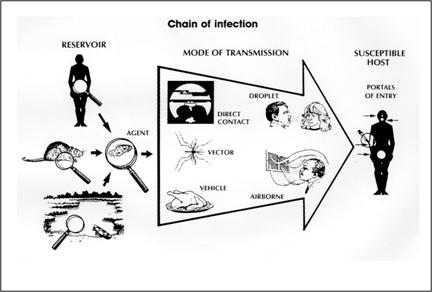
\includegraphics[width=0.5\linewidth]{figures/infection} 

}

\caption{Chain of infection. Source: Centers for Disease Control and Prevention [@dicker1992principles].}\label{fig:infection}
\end{figure}

\subsection{Data visualization}\label{data-visualization}

Data visualization or information visualization always played a crucial
role in scientific analysis. In many infectious disease studies, data
visualization could be a good starting point for the users to understand
how far the disease will spread and to illustrate our findings and
statistical insights. Besides, the ability to visualize, track, and
predict the spread of the disease can help raise awareness, understand
the impact of the disease, and ultimately assist in prevention efforts.

Data visualization is having a big moment during the COVID-19 pandemic.
Social media feeds are overwhelmed with infection heat maps and charts
depicting transmission patterns. We have all seen models projecting the
spread of the novel coronavirus. The COVID-19 pandemic also poses new
challenges to data scientists, too, for its vast and rapid spread and
significant economic impact.

A lot of work has been done on visualizing COVID-19 data since the
outbreak of the pandemic. The daily counts of cases and deaths of
COVID-19 are crucial for understanding how this pandemic is spreading.
Thanks to the contribution of the data science communities across the
world, multiple sources provide the COVID-19 data with different
precision and focus. To clean the data, we first fetch data from various
sources and compile them into the same format for further comparison and
integration. Appendix B describes the data used in the examples, case
studies, and lab exercises in the book.

R offers the opportunity to scale and automate tasks, document and track
them, and reliably reproduce their output. The first few chapters
investigate existing R visualization techniques used to manipulate and
represent infectious disease data. Chapter \ref{dplyr} provides an
introduction to data wrangling and how to use R packages \texttt{dplyr}
and \texttt{tidyr} to manipulate your data in a useful form for
visualization and modeling. This chapter is for someone who is already
somewhat familiar with \texttt{R}, but would like to know more about
using it for fundamental data analysis and manipulation.

\begin{figure}

{\centering 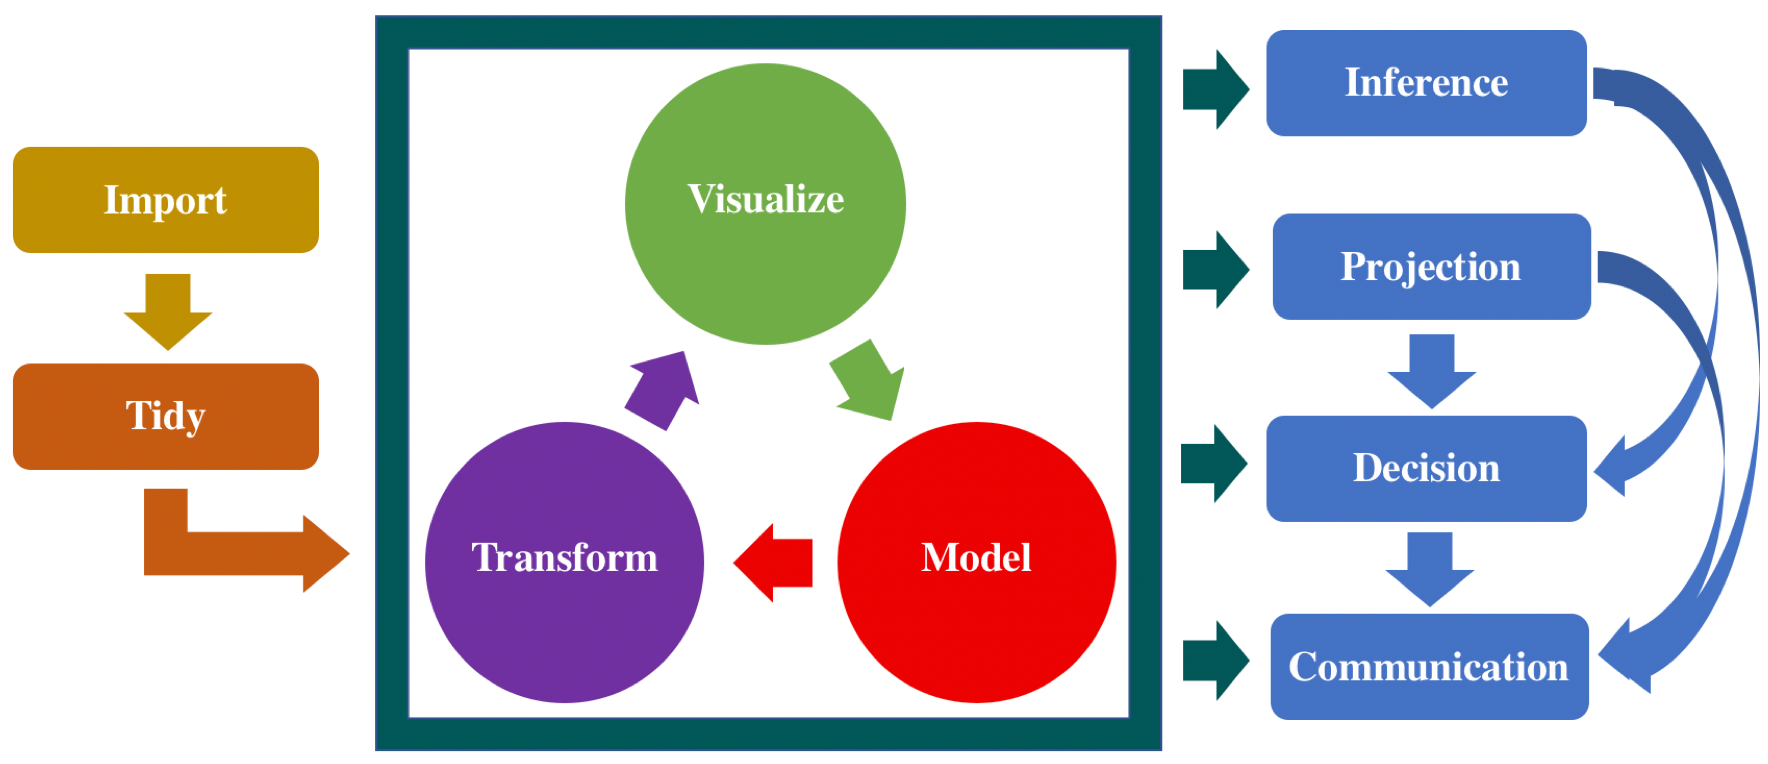
\includegraphics[width=0.7\linewidth]{figures/process} 

}

\caption{The stages of a data science workflow. Original source: @wickham2016r}\label{fig:process}
\end{figure}

Graphs can be presented using a variety of media: print, projection,
dashboard, etc. The visualizations can be primarily classified into two
groups: visualization with zero or less interactivity represents the
first group, and complex interactive visualization techniques and tools
represent the second. See Figure \ref{fig:plottypes} for different types
of visualization. Before constructing any display of epidemiologic data,
it is important to first determine the point to be conveyed and which
media you want to use for communications

\begin{figure}

{\centering 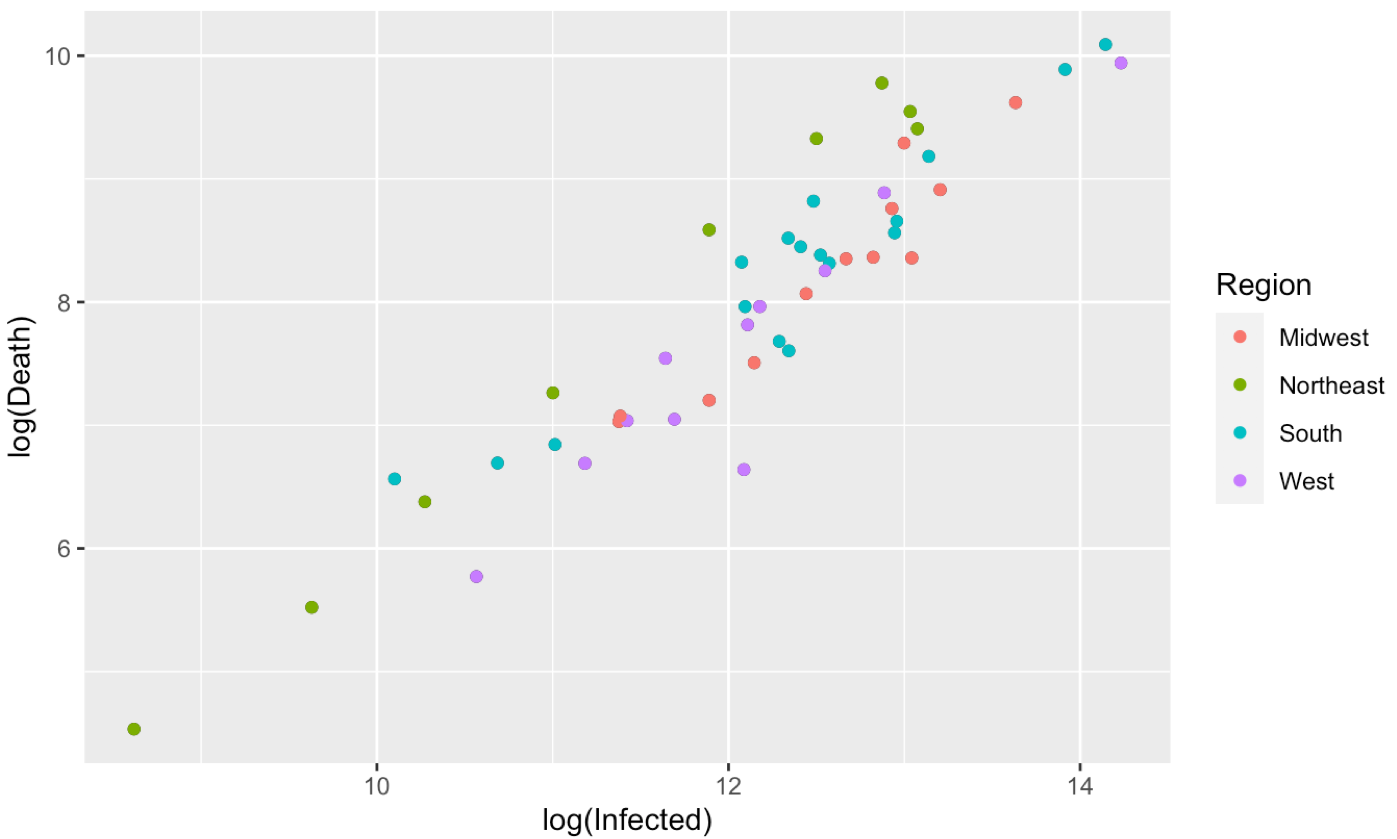
\includegraphics[width=0.4\linewidth]{figures/static_plot} 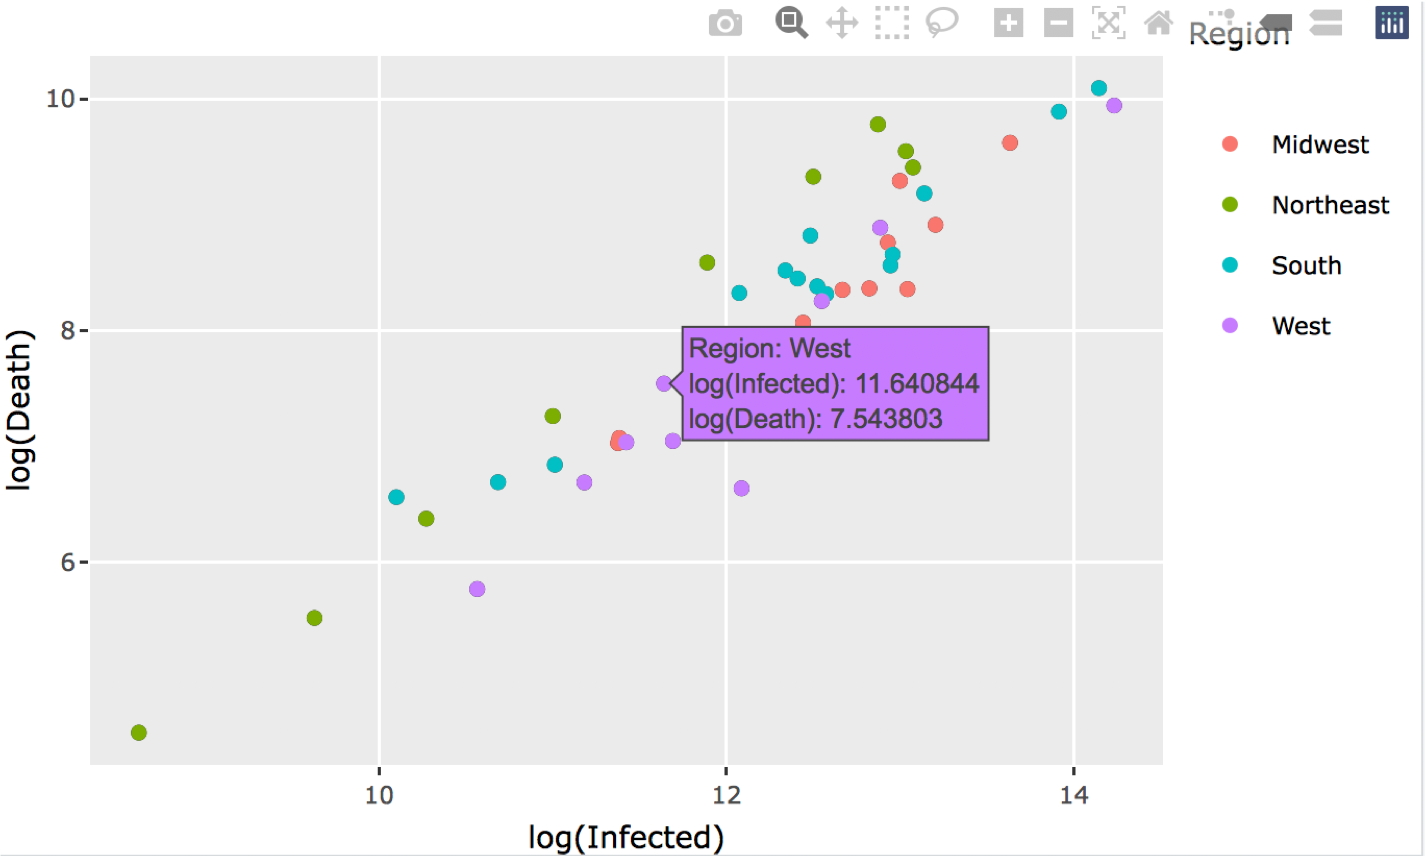
\includegraphics[width=0.4\linewidth]{figures/plotly_plot} 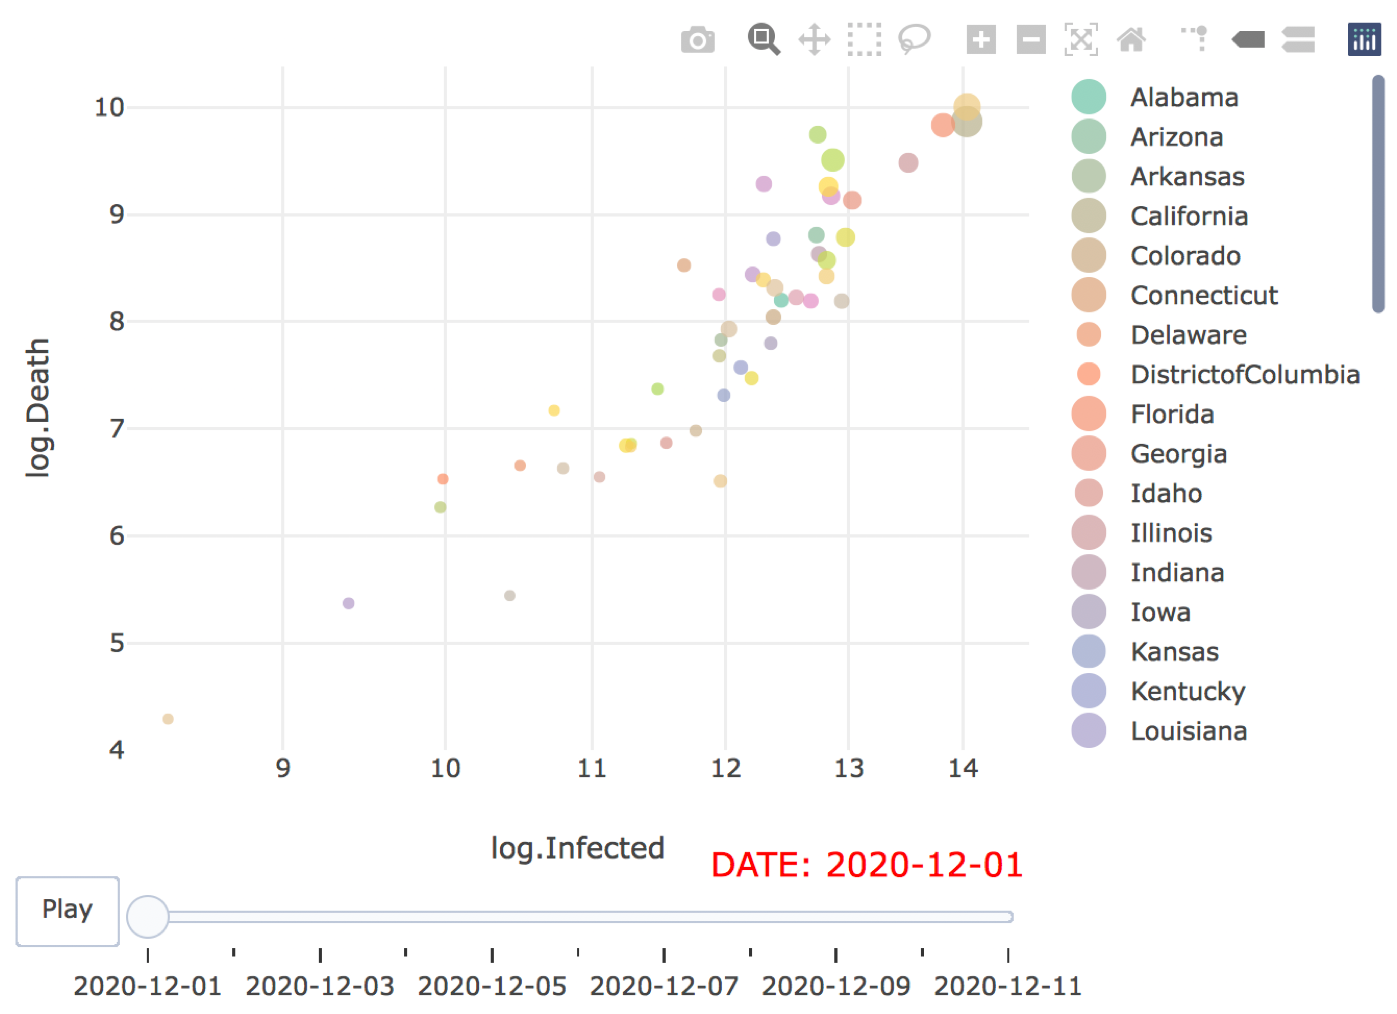
\includegraphics[width=0.4\linewidth]{figures/animation2} 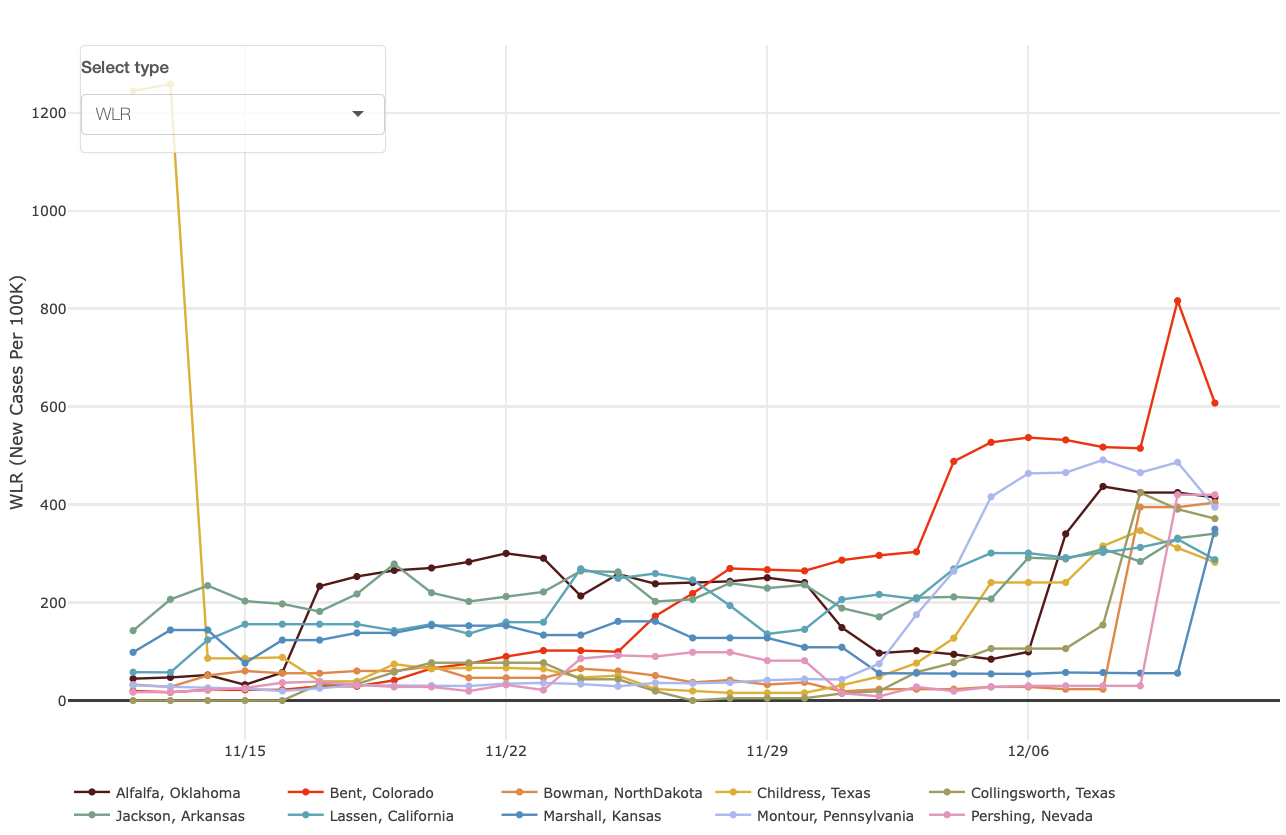
\includegraphics[width=0.4\linewidth]{figures/county_risk_ts} 

}

\caption{Types of visualization plots.}\label{fig:plottypes}
\end{figure}

Chapter \ref{ggplot2} introduces static visualization, which uses basic
graphs such as bar and line graphs for representing attributes of the
COVID-19 dataset. We use a collection of graphs for comparing cumulative
or daily new cases and deaths between states/counties in the US.

Chapter \ref{plotly} provide insight and practical skills for creating
interactive and dynamic web graphics for data analysis from R. This kind
of visualizations allow user interaction like hovering the mouse over
bars and points in the charts. It makes heavy use of \texttt{plotly} for
rendering graphics, but you'll also learn about other R packages that
augment a data science workflow, such as the \texttt{tidyverse} and
\texttt{shiny}. Along the way, you'll gain insight into best practices
for visualization of infectious disease data, statistical graphics, and
graphical perception. Chapter \ref{shiny} focuses on linking
\texttt{plotly} graphs with \texttt{shiny}, an open-source R package
that provides an elegant and powerful web framework for building web
applications. Chapter \ref{map} is an in-depth look at visualizing data
in a spatial setting and presenting findings through some geospatial
visualization.

\subsection{Modeling and Forecasting}\label{modeling-and-forecasting}

The concepts and techniques discussed in Chapters
\ref{dplyr}--\ref{shiny} have dealt with describing, visualizing, and
exploring the data. The use of scientific models for understanding the
dynamics of infectious diseases has a very rich history in epidemiology.

Starting in December 2019 in China, the outbreak of COVID-19 has spread
globally within weeks. To efficiently combat COVID-19, it is crucial to
have a better understanding of how far the virus will spread, and how
many lives it will claim. Scientific modeling is an essential tool to
answer these questions and ultimately assist in disease prevention,
policymaking, and resource allocation.

Chapter \ref{modeling} presents a few classic epidemic modeling
approaches, and takes the reader through steps required for fundamental
infectious data analysis and presentation of data typically encountered
in epidemiology using COVID-19 data set. Chapter \ref{regression}
introduces the analytical techniques of regression and discrimination as
a means of quantifying the effect of a set of explanatory variables on
the spatial distribution of a particular outcome.

Chapter \ref{timeseries} takes the reader through time series modeling
and forecasting. Chapter \ref{NN} introduces some neural network models
for forecasting. Chapter \ref{ensemble} describes the ensemble methods
using multiple forecasting algorithms to improve the predictive
performance.

\chapter{\texorpdfstring{Data Wrangling with \texttt{dplyr} and
\texttt{tidyr}}{Data Wrangling with dplyr and tidyr}}\label{dplyr}

The package \texttt{dplyr} is an R package for making tabular data
wrangling easier by using a limited set of functions that can be
combined to extract and summarize insights from your data. It pairs
nicely with the package \texttt{tidyr}, enabling you to swiftly convert
between different data formats (long vs.~wide) for plotting and
analysis. It addresses the common problem of reshaping your data for
plotting and use by different R functions. Sometimes we want data sets
where we have one row per measurement. Sometimes we want a dataframe
where each measurement type has its own column, and rows are instead
more aggregated groups. Sometimes you may want to select important
variables, filter out key observations, create new variables and obtain
summary statistics. As illustrated in Figure \ref{fig:process1}, you may
need to work back and forth between these formats, which is nontrivial,
and \texttt{tidyr} and \texttt{dplyr} give you the right tools for this
and more sophisticated data wrangling.

\begin{figure}

{\centering 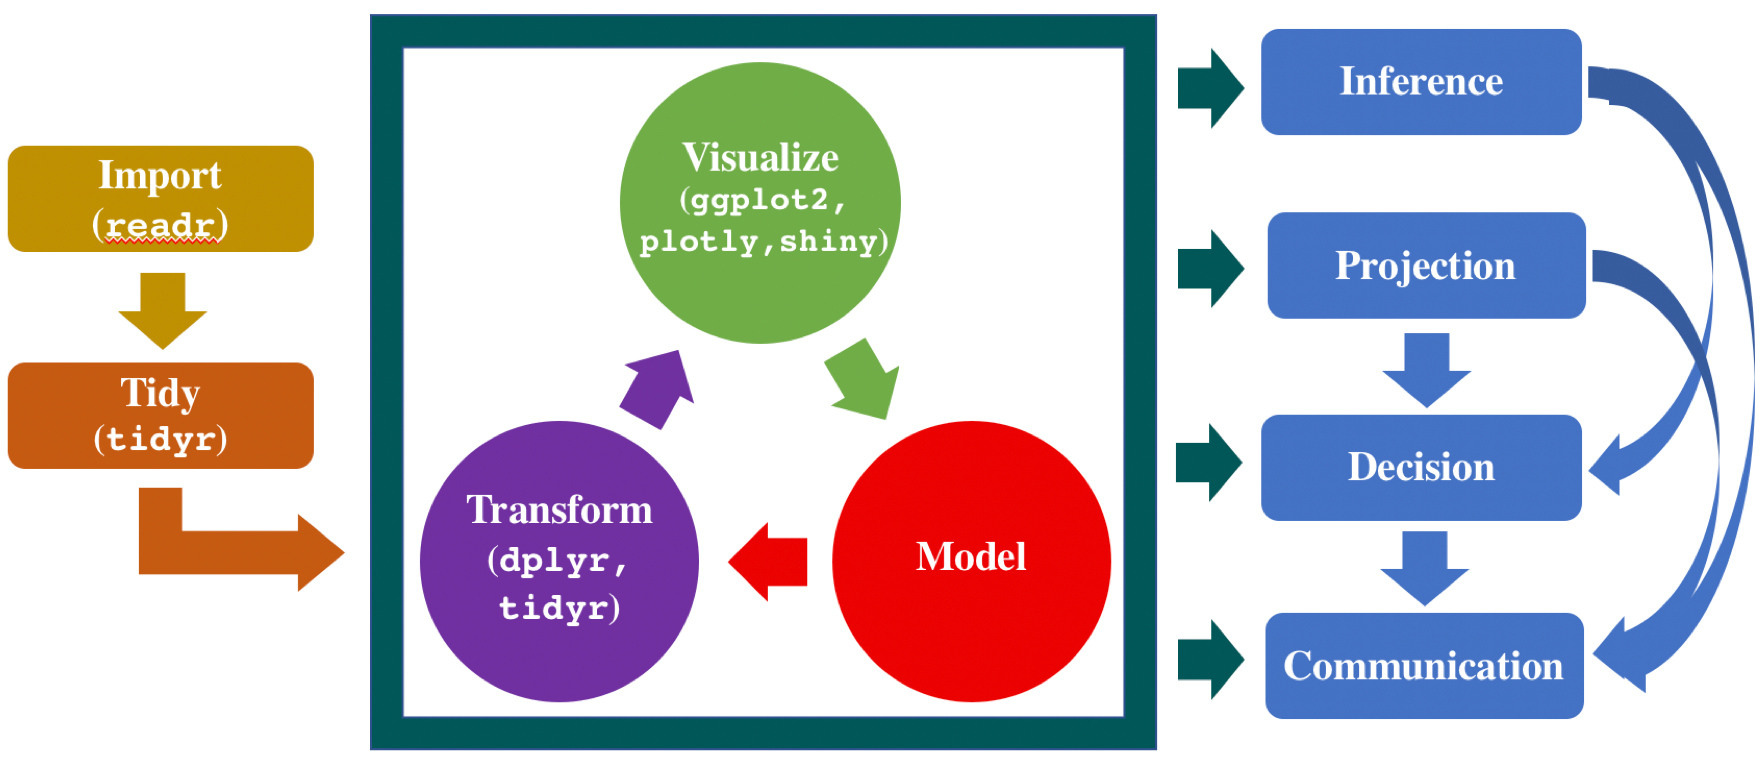
\includegraphics[width=0.75\linewidth]{figures/process_new} 

}

\caption{A typical data science process.}\label{fig:process1}
\end{figure}

The packages \texttt{dplyr} and \texttt{tidyr} are built to work
directly with data frames. In this chapter, you will learn how to use
these packages to perform data manipulation and transform your data into
the appropriate form.

\section{\texorpdfstring{Learning
\texttt{dplyr}}{Learning dplyr}}\label{learning-dplyr}

\begin{Shaded}
\begin{Highlighting}[]
\CommentTok{# load the packages}
\KeywordTok{library}\NormalTok{(tidyverse)}
\end{Highlighting}
\end{Shaded}

\begin{verbatim}
## -- Attaching packages ------------------- tidyverse 1.3.0 --
\end{verbatim}

\begin{verbatim}
## v ggplot2 3.3.3     v purrr   0.3.4
## v tibble  3.0.5     v dplyr   1.0.3
## v tidyr   1.1.2     v stringr 1.4.0
## v readr   1.4.0     v forcats 0.5.1
\end{verbatim}

\begin{verbatim}
## -- Conflicts ---------------------- tidyverse_conflicts() --
## x dplyr::filter() masks stats::filter()
## x dplyr::lag()    masks stats::lag()
\end{verbatim}

\begin{Shaded}
\begin{Highlighting}[]
\KeywordTok{library}\NormalTok{(dplyr)}
\end{Highlighting}
\end{Shaded}

\subsection{Tibbles}\label{tibbles}

Throughout this book, we work with ``tibbles'' instead of R's
traditional ``data.frame''. Tibbles are data frames, but they are a
modern reimagining of the ``data.frame'', keeping what time has proven
to be effective, and throwing out what is not. Here we will use the
\texttt{tibble} package, which provides opinionated data frames that
make working in the \texttt{tidyverse} a little easier.

\begin{Shaded}
\begin{Highlighting}[]
\CommentTok{# The easiest way to get tibble is to install the whole tidyverse:}
 \KeywordTok{install.packages}\NormalTok{(}\StringTok{"tidyverse"}\NormalTok{)}

\CommentTok{# Alternatively, install just tibble:}
\KeywordTok{install.packages}\NormalTok{(}\StringTok{"tibble"}\NormalTok{)}
\end{Highlighting}
\end{Shaded}

In most places, we will use the term ``tibble'' and ``data frame''
interchangeably; when we want to draw particular attention to R's
built-in data frame, we will call them ``data.frame''. See
\citet{wickham2016r} for more details about how to create and use
``tibbles''.

\subsection{Import data}\label{import-data}

Recall R offers many ways to import data:

\begin{itemize}
\item
  \texttt{read\_csv()} reads comma delimited files,
  \texttt{read\_csv2()} reads semicolon separated files.
\item
  \texttt{read\_tsv()} reads tab delimited files, and
  \texttt{read\_delim()} reads in files with any delimiter.
\item
  \texttt{read\_fwf()} reads fixed width files. You can specify fields
  either by their widths with \texttt{fwf\_widths()} or their position
  with \texttt{fwf\_positions()}.
\item
  \texttt{read\_table()} reads a common variation of fixed width files
  where columns are separated by white space.
\item
  \texttt{load()} loads an \texttt{.RData} file and import all of the
  objects contained in the \texttt{.RData} file into your current
  workspace.
\end{itemize}

Below we will work on COVID-19 county level infected count data
(\texttt{I.county}), and we can obtain the data from Github R package
\texttt{slid}. It is a ``data frame'' which includes ``ID''
(county-level Federal Information Processing System code), ``County''
(name of county), ``State'' (name of state), ``XYYYY.MM.DD'' (the number
of cumulative infected cases in a county related to the date of
YYYY.MM.DD) for 3,104 counties in the US. For example, the variable
\texttt{X2020.01.22} is the number of cumulative infected cases in a
county on 01/22/2020. See Appendix B for more detailed description of
the data and its source.

\begin{Shaded}
\begin{Highlighting}[]
\CommentTok{# install the slid package from github}
\CommentTok{# library(devtools)}
\CommentTok{# devtools::install_github('covid19-dashboard-us/slid')}
\CommentTok{# load objects in I.county into my workspace}
\KeywordTok{library}\NormalTok{(slid)}
\KeywordTok{data}\NormalTok{(I.county)}

\CommentTok{# make I.county a tibble with as_tibble()}
\NormalTok{I.county <-}\StringTok{ }\KeywordTok{as_tibble}\NormalTok{(I.county)}

\CommentTok{# preview the data}
\CommentTok{# View(I.county)}
\end{Highlighting}
\end{Shaded}

\subsection{\texorpdfstring{Common \texttt{dplyr}
functions}{Common dplyr functions}}\label{common-dplyr-functions}

Next, we will learn some of the most common \texttt{dplyr} functions:

\begin{itemize}
\tightlist
\item
  \texttt{select()}: subset columns;
\item
  \texttt{filter()}: subset rows on conditions;
\item
  \texttt{mutate()}: create new columns by using information from other
  columns;
\item
  \texttt{group\_by()} and \texttt{summarize()}: create summary
  statistics on grouped data;
\item
  \texttt{arrange()}: sort results;
\item
  \texttt{join()} family: combine datasets.
\end{itemize}

A typical code structure of \texttt{dplyr} is:

\begin{Shaded}
\begin{Highlighting}[]
\NormalTok{data.new <-}\StringTok{ }\NormalTok{data.original }\OperatorTok
\StringTok{  }\NormalTok{select rows or columns to manipulate }\OperatorTok
\StringTok{  }\NormalTok{arrange or group the data }\OperatorTok
\StringTok{  }\NormalTok{summarize the data}
\end{Highlighting}
\end{Shaded}

The first argument is a data frame, and the subsequent arguments
separated by \texttt{\%\textgreater{}\%} describe the data manipulation
and/or summary, and the result is a new data frame. We will explain more
details in the following sections.

\section{Selecting Columns and Filtering
Rows}\label{selecting-columns-and-filtering-rows}

\subsection{Subset Variables (Columns)}\label{subset-variables-columns}

To select columns of a dataframe, use \texttt{select()}. The first
argument to this function is the data frame (\texttt{I.county}), and the
subsequent arguments are the columns to keep, separated by commas.
Alternatively, if you are selecting columns adjacent to each other, you
can use a \texttt{:} to select a range of columns, read as ``select
columns from \_\_ to \_\_''.

\begin{Shaded}
\begin{Highlighting}[]
\CommentTok{# load the tidyverse}
\NormalTok{dplyr}\OperatorTok{::}\KeywordTok{select}\NormalTok{(I.county, ID, County, State)}
\CommentTok{# select a series of connected columns}
\NormalTok{dplyr}\OperatorTok{::}\KeywordTok{select}\NormalTok{(I.county, ID, County, State, X2020.}\FloatTok{12.11}\OperatorTok{:}\NormalTok{X2020.}\FloatTok{12.01}\NormalTok{)}
\end{Highlighting}
\end{Shaded}

\subsection{Subset Observations (Rows)}\label{subset-observations-rows}

To choose rows based on specific criteria, we can use the
\texttt{filter()} function. The arguments after the dataframe are the
condition(s) we want for our final dataframe to adhere to (e.g.
\texttt{State} name is ``Iowa''). We can chain a series of conditions
together using commas between each condition.

\begin{Shaded}
\begin{Highlighting}[]
\CommentTok{# all Iowa counties}
\NormalTok{dplyr}\OperatorTok{::}\KeywordTok{filter}\NormalTok{(I.county, State }\OperatorTok{==}\StringTok{ "Iowa"}\NormalTok{)}
\end{Highlighting}
\end{Shaded}

Here is an example of \texttt{filter()} function with multiple
conditions:

\begin{Shaded}
\begin{Highlighting}[]
\CommentTok{# all Iowa counties with cumulative infection count > 10000}
\NormalTok{dplyr}\OperatorTok{::}\KeywordTok{filter}\NormalTok{(I.county, State }\OperatorTok{==}\StringTok{ "Iowa"}\NormalTok{, X2020.}\FloatTok{12.11} \OperatorTok{>}\StringTok{ }\DecValTok{10000}\NormalTok{)}
\end{Highlighting}
\end{Shaded}

To use filtering effectively, it is better to know some of the
comparison and logical operators. Figure \ref{fig:logic} shows some
commonly used R logic comparisons:

\begin{figure}

{\centering 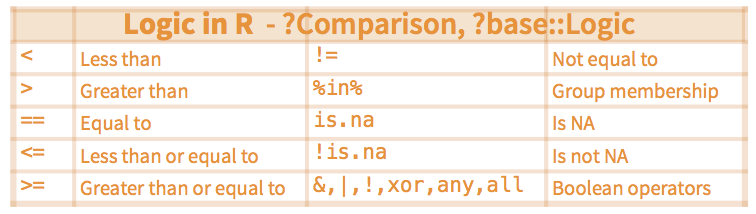
\includegraphics[width=0.75\linewidth]{figures/logic} 

}

\caption{Some commonly used logic comparisons.}\label{fig:logic}
\end{figure}

\subsection{Pipes}\label{pipes}

What if you want to select and filter at the same time? There are three
ways to do this: use intermediate steps, nested functions, or pipes.

With intermediate steps, you create a temporary dataframe and use that
as input to the next function, like this:

\begin{Shaded}
\begin{Highlighting}[]
\CommentTok{# all Iowa counties from 2020.12.01 to 2020.12.11}
\CommentTok{# method 1}
\NormalTok{Iowa.I.county <-}\StringTok{ }\NormalTok{dplyr}\OperatorTok{::}\KeywordTok{filter}\NormalTok{(I.county, State }\OperatorTok{==}\StringTok{ "Iowa"}\NormalTok{)}
\NormalTok{Iowa.I.county.DEC <-}\StringTok{ }\NormalTok{dplyr}\OperatorTok{::}\KeywordTok{select}\NormalTok{(Iowa.I.county, }
\NormalTok{                                   X2020.}\FloatTok{12.11}\OperatorTok{:}\NormalTok{X2020.}\FloatTok{12.01}\NormalTok{)}
\end{Highlighting}
\end{Shaded}

This is readable, but can clutter up your workspace with lots of objects
that you have to name individually. With multiple steps, that can be
hard to keep track of.

You can also nest functions (i.e.~one function inside of another), like
this:

\begin{Shaded}
\begin{Highlighting}[]
\CommentTok{# all Iowa counties from 2020.12.01 to 2020.12.11}
\CommentTok{# method 2}
\NormalTok{Iowa.I.county.DEC <-}\StringTok{ }
\StringTok{  }\NormalTok{dplyr}\OperatorTok{::}\KeywordTok{select}\NormalTok{(dplyr}\OperatorTok{::}\KeywordTok{filter}\NormalTok{(I.county, State }\OperatorTok{==}\StringTok{ "Iowa"}\NormalTok{), }
\NormalTok{                ID, County, State, X2020.}\FloatTok{12.11}\OperatorTok{:}\NormalTok{X2020.}\FloatTok{12.01}\NormalTok{)}
\end{Highlighting}
\end{Shaded}

This is handy but can be difficult to read if too many functions are
nested, as R evaluates the expression from the inside out (in this case,
filtering, then selecting).

The last option, \textbf{pipes}, are a recent addition to R.
\textbf{Pipes} let you take the output of one function and send it
directly to the next, which is useful when you need to do many things to
the same dataset. Pipes in R look like \texttt{\%\textgreater{}\%} and
are made available via the \texttt{magrittr} package, installed
automatically with \texttt{dplyr}.

\begin{Shaded}
\begin{Highlighting}[]
\CommentTok{# all Iowa counties from 2020.12.01 to 2020.12.11}
\CommentTok{# method 3}
\NormalTok{I.county }\OperatorTok
\StringTok{  }\NormalTok{dplyr}\OperatorTok{::}\KeywordTok{filter}\NormalTok{(State }\OperatorTok{==}\StringTok{ "Iowa"}\NormalTok{) }\OperatorTok
\StringTok{  }\NormalTok{dplyr}\OperatorTok{::}\KeywordTok{select}\NormalTok{(ID, County, X2020.}\FloatTok{12.11}\OperatorTok{:}\NormalTok{X2020.}\FloatTok{12.01}\NormalTok{)}
\end{Highlighting}
\end{Shaded}

In the above code, we use the \textbf{pipe} to send the interviews
dataset first through \texttt{filter()} to keep rows for the state of
Iowa, then through \texttt{select()} to keep only the count in December.
Since \texttt{\%\textgreater{}\%} takes the object on its left and
passes it as the first argument to the function on its right, we don't
need to explicitly include the \texttt{dataframe} as an argument to the
\texttt{filter()} and \texttt{select()} functions anymore.

Some may find it helpful to read the pipe like the word ``then''. For
instance, in the above example, we take the dataframe \texttt{I.county},
then we filter for rows with \texttt{State\ ==\ "Iowa"}, then we select
columns from \texttt{X2020.12.11} to \texttt{X2020.12.01}. The
\texttt{dplyr} functions are somewhat simple, but by combining them into
linear workflows with the pipe, we can accomplish more complex data
wrangling operations.

If we want to create a new object with this smaller version of the data,
we can assign it a new name:

\begin{Shaded}
\begin{Highlighting}[]
\CommentTok{# assign a name to all Iowa counties }
\CommentTok{# from 2020.12.01 to 2020.12.11}
\NormalTok{Iowa.I.county.DEC <-}\StringTok{ }\NormalTok{I.county }\OperatorTok
\StringTok{  }\NormalTok{dplyr}\OperatorTok{::}\KeywordTok{filter}\NormalTok{(State }\OperatorTok{==}\StringTok{ "Iowa"}\NormalTok{) }\OperatorTok
\StringTok{    }\NormalTok{dplyr}\OperatorTok{::}\KeywordTok{select}\NormalTok{(ID, County, X2020.}\FloatTok{12.11}\OperatorTok{:}\NormalTok{X2020.}\FloatTok{12.01}\NormalTok{)}

\KeywordTok{head}\NormalTok{(Iowa.I.county.DEC)}
\end{Highlighting}
\end{Shaded}

\begin{verbatim}
## # A tibble: 6 x 13
##      ID County X2020.12.11 X2020.12.10 X2020.12.09
##   <int> <fct>        <int>       <int>       <int>
## 1 19001 Adair          506         503         499
## 2 19003 Adams          208         206         200
## 3 19005 Allam~         995         990         971
## 4 19007 Appan~         868         862         858
## 5 19009 Audub~         326         323         321
## 6 19011 Benton        1852        1847        1826
## # ... with 8 more variables: X2020.12.08 <int>,
## #   X2020.12.07 <int>, X2020.12.06 <int>,
## #   X2020.12.05 <int>, X2020.12.04 <int>,
## #   X2020.12.03 <int>, X2020.12.02 <int>, X2020.12.01 <int>
\end{verbatim}

\subsection{Select and order top n entries (by group if grouped
data).}\label{select-and-order-top-n-entries-by-group-if-grouped-data.}

The function \texttt{top\_n} can be used to select top (or bottom) n
rows (by value).

This is a convenient wrapper that uses \texttt{filter()}and
\texttt{min\_rank()} to select the top or bottom entries in each group,
ordered by \texttt{wt}.

\textbf{Usage}

\begin{Shaded}
\begin{Highlighting}[]
\KeywordTok{top_n}\NormalTok{(x, n, wt)}
\end{Highlighting}
\end{Shaded}

\textbf{Arguments}

\begin{itemize}
\tightlist
\item
  \texttt{x}: a \texttt{tbl()} to filter
\item
  \texttt{n}: number of rows to return. If \texttt{x} is grouped, this
  is the number of rows per group. Will include more than \texttt{n}
  rows if there are ties. If \texttt{n} is positive, selects the top
  \texttt{n} rows. If negative, selects the bottom \texttt{n} rows.
\item
  \texttt{wt} (Optional). The variable to use for ordering. If not
  specified, defaults to the last variable in the \texttt{tbl}.
\end{itemize}

This argument is automatically quoted and later evaluated in the context
of the data frame. It supports unquoting.

Let us find the top ten counties with the largest cumulative infected
count on December 11, 2020.

\begin{Shaded}
\begin{Highlighting}[]
\CommentTok{# top ten counties with the cum. infected count}
\NormalTok{I.county.top10 <-}\StringTok{ }\NormalTok{I.county }\OperatorTok\StringTok{ }\KeywordTok{top_n}\NormalTok{(}\DecValTok{10}\NormalTok{, }\DataTypeTok{wt =}\NormalTok{ X2020.}\FloatTok{12.11}\NormalTok{)}
\NormalTok{I.county.top10}\OperatorTok{$}\NormalTok{County}
\end{Highlighting}
\end{Shaded}

\begin{verbatim}
##  [1] Maricopa      LosAngeles    SanBernardino Broward      
##  [5] Miami-Dade    Cook          Clark         Dallas       
##  [9] Harris        Tarrant      
## 1839 Levels: Abbeville AcadiaParish Accomack Ada ... obrien
\end{verbatim}

Let us find the bottom ten counties with the smallest cumulative
infected count on December 11, 2020.

\begin{Shaded}
\begin{Highlighting}[]
\CommentTok{# bottom ten counties with the cum. infected count}
\NormalTok{I.county.bottom10 <-}\StringTok{ }\NormalTok{I.county }\OperatorTok\StringTok{ }\KeywordTok{top_n}\NormalTok{(}\OperatorTok{-}\DecValTok{10}\NormalTok{, }\DataTypeTok{wt =}\NormalTok{ X2020.}\FloatTok{12.11}\NormalTok{)}
\NormalTok{I.county.bottom10}\OperatorTok{$}\NormalTok{County}
\end{Highlighting}
\end{Shaded}

\begin{verbatim}
##  [1] Dukes        Nantucket    OglalaLakota Beaver      
##  [5] BoxElder     Cache        Carbon       Daggett     
##  [9] Duchesne     Emery        Garfield     Grand       
## [13] Iron         Juab         Kane         Millard     
## [17] Morgan       Piute        Rich         Sanpete     
## [21] Sevier       Uintah       Washington   Wayne       
## [25] Weber       
## 1839 Levels: Abbeville AcadiaParish Accomack Ada ... obrien
\end{verbatim}

Let us find the county with the largest cumulative infected count on
December 11, 2020 for each state.

\begin{Shaded}
\begin{Highlighting}[]
\CommentTok{# county with the largest cum. infected count for each state}
\NormalTok{I.county.top1 <-}\StringTok{ }\NormalTok{I.county }\OperatorTok\StringTok{ }
\StringTok{  }\KeywordTok{group_by}\NormalTok{(State) }\OperatorTok
\StringTok{  }\KeywordTok{top_n}\NormalTok{(}\DecValTok{1}\NormalTok{, }\DataTypeTok{wt =}\NormalTok{ X2020.}\FloatTok{12.11}\NormalTok{) }\OperatorTok\StringTok{ }
\StringTok{  }\NormalTok{dplyr}\OperatorTok{::}\KeywordTok{select}\NormalTok{(State, County)}
\end{Highlighting}
\end{Shaded}

\section{Make New Variables: Mutate}\label{make-new-variables-mutate}

Frequently you will want to create new columns based on the values in
existing columns, for example, to obtain the number of daily new cases
based on the cumulative count. For this, we can use the
\texttt{mutate()} function.

\begin{Shaded}
\begin{Highlighting}[]
\CommentTok{# create a new variable Y2020.12.11 (new count 2020.12.11)}
\NormalTok{I.county.new <-}\StringTok{ }\NormalTok{I.county }\OperatorTok\StringTok{ }
\StringTok{    }\NormalTok{dplyr}\OperatorTok{::}\KeywordTok{filter}\NormalTok{(State }\OperatorTok{==}\StringTok{ "Iowa"}\NormalTok{) }\OperatorTok
\StringTok{    }\NormalTok{dplyr}\OperatorTok{::}\KeywordTok{select}\NormalTok{(ID, County, X2020.}\FloatTok{12.11}\OperatorTok{:}\NormalTok{X2020.}\FloatTok{12.10}\NormalTok{) }\OperatorTok\StringTok{ }
\StringTok{    }\KeywordTok{mutate}\NormalTok{(}\DataTypeTok{Y2020.12.11 =}\NormalTok{ X2020.}\FloatTok{12.11} \OperatorTok{-}\StringTok{ }\NormalTok{X2020.}\FloatTok{12.10}\NormalTok{)}

\KeywordTok{head}\NormalTok{(I.county.new)}
\end{Highlighting}
\end{Shaded}

\begin{verbatim}
## # A tibble: 6 x 5
##      ID County    X2020.12.11 X2020.12.10 Y2020.12.11
##   <int> <fct>           <int>       <int>       <int>
## 1 19001 Adair             506         503           3
## 2 19003 Adams             208         206           2
## 3 19005 Allamakee         995         990           5
## 4 19007 Appanoose         868         862           6
## 5 19009 Audubon           326         323           3
## 6 19011 Benton           1852        1847           5
\end{verbatim}

If we want to obtain the number of daily new cases based on the
cumulative count for the dates in December only, we can try the
following:

\begin{Shaded}
\begin{Highlighting}[]
\CommentTok{# create variables Y2020.12.01 : Y2020.12.11}
\CommentTok{# with daily new count}

\NormalTok{I.county.Iowa <-}\StringTok{ }\NormalTok{I.county }\OperatorTok\StringTok{ }
\StringTok{  }\NormalTok{dplyr}\OperatorTok{::}\KeywordTok{filter}\NormalTok{(State }\OperatorTok{==}\StringTok{ "Iowa"}\NormalTok{)}

\NormalTok{I.county.tmp <-}\StringTok{ }\NormalTok{I.county.Iowa[, }\OperatorTok{-}\NormalTok{(}\DecValTok{1}\OperatorTok{:}\DecValTok{3}\NormalTok{)]}
\NormalTok{I.county.Iowa.new <-}\StringTok{ }\NormalTok{I.county.Iowa}
\NormalTok{I.county.Iowa.new[, }\OperatorTok{-}\NormalTok{(}\DecValTok{1}\OperatorTok{:}\DecValTok{3}\NormalTok{)] <-}\StringTok{ }\NormalTok{I.county.tmp }\OperatorTok{-}\StringTok{ }
\StringTok{  }\KeywordTok{cbind}\NormalTok{(I.county.tmp[, }\OperatorTok{-}\DecValTok{1}\NormalTok{], }\DecValTok{0}\NormalTok{)}

\NormalTok{I.county.Iowa.DEC <-}\StringTok{ }\NormalTok{I.county.Iowa.new }\OperatorTok\StringTok{ }
\NormalTok{dplyr}\OperatorTok{::}\KeywordTok{select}\NormalTok{(ID, County, X2020.}\FloatTok{12.11}\OperatorTok{:}\NormalTok{X2020.}\FloatTok{12.01}\NormalTok{)  }

\NormalTok{name.tmp <-}\StringTok{ }\KeywordTok{substring}\NormalTok{(}\KeywordTok{names}\NormalTok{(I.county.Iowa.DEC)[}\OperatorTok{-}\NormalTok{(}\DecValTok{1}\OperatorTok{:}\DecValTok{2}\NormalTok{)], }\DecValTok{2}\NormalTok{)}
\KeywordTok{names}\NormalTok{(I.county.Iowa.DEC)[}\OperatorTok{-}\NormalTok{(}\DecValTok{1}\OperatorTok{:}\DecValTok{2}\NormalTok{)] <-}\StringTok{ }\KeywordTok{paste0}\NormalTok{(}\StringTok{"Y"}\NormalTok{, name.tmp)}
\KeywordTok{head}\NormalTok{(I.county.Iowa.DEC)}
\end{Highlighting}
\end{Shaded}

\begin{verbatim}
## # A tibble: 6 x 13
##      ID County Y2020.12.11 Y2020.12.10 Y2020.12.09
##   <int> <fct>        <int>       <int>       <int>
## 1 19001 Adair            3           4          10
## 2 19003 Adams            2           6           4
## 3 19005 Allam~           5          19          17
## 4 19007 Appan~           6           4           5
## 5 19009 Audub~           3           2           6
## 6 19011 Benton           5          21           7
## # ... with 8 more variables: Y2020.12.08 <int>,
## #   Y2020.12.07 <int>, Y2020.12.06 <int>,
## #   Y2020.12.05 <int>, Y2020.12.04 <int>,
## #   Y2020.12.03 <int>, Y2020.12.02 <int>, Y2020.12.01 <int>
\end{verbatim}

\section{Summarize Data}\label{summarize-data}

Many data analysis tasks can be approached using the split-apply-combine
paradigm: split the data into groups, apply some analysis to each group,
and then combine the results. \texttt{dplyr} makes this very easy via
the \texttt{group\_by()} function.

The \texttt{summarize()} function uses summary functions, functions that
take a vector of values and return a single value, such as:

\begin{itemize}
\tightlist
\item
  \texttt{dplyr::first}: first value of a vector.
\item
  \texttt{dplyr::last}: last value of a vector.
\item
  \texttt{dplyr::nth}: nth value of a vector.
\item
  \texttt{dplyr::n}: number of values in a vector.
\item
  \texttt{dplyr::n\_distinct}: number of distinct values in a vector.
\item
  \texttt{IQR}: IQR of a vector.
\item
  \texttt{min}: minimum value in a vector.
\item
  \texttt{max}: maximum value in a vector.
\item
  \texttt{mean}: mean value of a vector.
\item
  \texttt{median}: median value of a vector.
\item
  \texttt{var}: variance of a vector.
\item
  \texttt{sd}: standard deviation of a vector.
\end{itemize}

The \texttt{group\_by()} function is often used together with
\texttt{summarize()}, which collapses each group into a single-row
summary of that group. The \texttt{group\_by()} takes as arguments the
column names that contain the categorical variables for which you want
to calculate the summary statistics. Once the data are grouped, you can
also summarize multiple variables simultaneously (and not necessarily on
the same variable). So to compute the state level cumulative infected
count by \texttt{State}:

\begin{Shaded}
\begin{Highlighting}[]
\CommentTok{# state level cumulative infected count}
\CommentTok{# method 1: summarize()}
\NormalTok{I.state <-}\StringTok{ }\NormalTok{I.county }\OperatorTok
\StringTok{  }\KeywordTok{group_by}\NormalTok{(State) }\OperatorTok
\StringTok{  }\KeywordTok{summarize}\NormalTok{(}\KeywordTok{across}\NormalTok{(X2020.}\FloatTok{12.11}\OperatorTok{:}\NormalTok{X2020.}\FloatTok{01.22}\NormalTok{, }
                   \OperatorTok{~}\StringTok{ }\KeywordTok{sum}\NormalTok{(.x, }\DataTypeTok{na.rm =} \OtherTok{TRUE}\NormalTok{)))}
\KeywordTok{head}\NormalTok{(I.state, }\DecValTok{2}\NormalTok{)}
\end{Highlighting}
\end{Shaded}

\begin{verbatim}
## # A tibble: 2 x 326
##   State X2020.12.11 X2020.12.10 X2020.12.09 X2020.12.08
##   <fct>       <int>       <int>       <int>       <int>
## 1 Alab~      288775      284922      280187      276665
## 2 Ariz~      394512      387529      382601      378157
## # ... with 321 more variables: X2020.12.07 <int>,
## #   X2020.12.06 <int>, X2020.12.05 <int>,
## #   X2020.12.04 <int>, X2020.12.03 <int>,
## #   X2020.12.02 <int>, X2020.12.01 <int>,
## #   X2020.11.30 <int>, X2020.11.29 <int>,
## #   X2020.11.28 <int>, X2020.11.27 <int>,
## #   X2020.11.26 <int>, X2020.11.25 <int>,
## #   X2020.11.24 <int>, X2020.11.23 <int>,
## #   X2020.11.22 <int>, X2020.11.21 <int>,
## #   X2020.11.20 <int>, X2020.11.19 <int>,
## #   X2020.11.18 <int>, X2020.11.17 <int>,
## #   X2020.11.16 <int>, X2020.11.15 <int>,
## #   X2020.11.14 <int>, X2020.11.13 <int>,
## #   X2020.11.12 <int>, X2020.11.11 <int>,
## #   X2020.11.10 <int>, X2020.11.09 <int>,
## #   X2020.11.08 <int>, X2020.11.07 <int>,
## #   X2020.11.06 <int>, X2020.11.05 <int>,
## #   X2020.11.04 <int>, X2020.11.03 <int>,
## #   X2020.11.02 <int>, X2020.11.01 <int>,
## #   X2020.10.31 <int>, X2020.10.30 <int>,
## #   X2020.10.29 <int>, X2020.10.28 <int>,
## #   X2020.10.27 <int>, X2020.10.26 <int>,
## #   X2020.10.25 <int>, X2020.10.24 <int>,
## #   X2020.10.23 <int>, X2020.10.22 <int>,
## #   X2020.10.21 <int>, X2020.10.20 <int>,
## #   X2020.10.19 <int>, X2020.10.18 <int>,
## #   X2020.10.17 <int>, X2020.10.16 <int>,
## #   X2020.10.15 <int>, X2020.10.14 <int>,
## #   X2020.10.13 <int>, X2020.10.12 <int>,
## #   X2020.10.11 <int>, X2020.10.10 <int>,
## #   X2020.10.09 <int>, X2020.10.08 <int>,
## #   X2020.10.07 <int>, X2020.10.06 <int>,
## #   X2020.10.05 <int>, X2020.10.04 <int>,
## #   X2020.10.03 <int>, X2020.10.02 <int>,
## #   X2020.10.01 <int>, X2020.09.30 <int>,
## #   X2020.09.29 <int>, X2020.09.28 <int>,
## #   X2020.09.27 <int>, X2020.09.26 <int>,
## #   X2020.09.25 <int>, X2020.09.24 <int>,
## #   X2020.09.23 <int>, X2020.09.22 <int>,
## #   X2020.09.21 <int>, X2020.09.20 <int>,
## #   X2020.09.19 <int>, X2020.09.18 <int>,
## #   X2020.09.17 <int>, X2020.09.16 <int>,
## #   X2020.09.15 <int>, X2020.09.14 <int>,
## #   X2020.09.13 <int>, X2020.09.12 <int>,
## #   X2020.09.11 <int>, X2020.09.10 <int>,
## #   X2020.09.09 <int>, X2020.09.08 <int>,
## #   X2020.09.07 <int>, X2020.09.06 <int>,
## #   X2020.09.05 <int>, X2020.09.04 <int>,
## #   X2020.09.03 <int>, X2020.09.02 <int>,
## #   X2020.09.01 <int>, X2020.08.31 <int>,
## #   X2020.08.30 <int>, ...
\end{verbatim}

or we can use \texttt{summarize\_at()}, which affects variables selected
with a character vector or \texttt{vars()}:

\begin{Shaded}
\begin{Highlighting}[]
\CommentTok{# state level cumulative infected count}
\CommentTok{# method 2: summarize_at()}
\NormalTok{I.state <-}\StringTok{ }\NormalTok{I.county }\OperatorTok
\StringTok{  }\KeywordTok{group_by}\NormalTok{(State) }\OperatorTok
\StringTok{  }\KeywordTok{summarize_at}\NormalTok{(}\KeywordTok{vars}\NormalTok{(X2020.}\FloatTok{12.11}\OperatorTok{:}\NormalTok{X2020.}\FloatTok{01.22}\NormalTok{), }
               \OperatorTok{~}\StringTok{ }\KeywordTok{sum}\NormalTok{(.x, }\DataTypeTok{na.rm =} \OtherTok{TRUE}\NormalTok{))}

\KeywordTok{head}\NormalTok{(I.state, }\DecValTok{2}\NormalTok{)}
\end{Highlighting}
\end{Shaded}

\begin{verbatim}
## # A tibble: 2 x 326
##   State X2020.12.11 X2020.12.10 X2020.12.09 X2020.12.08
##   <fct>       <int>       <int>       <int>       <int>
## 1 Alab~      288775      284922      280187      276665
## 2 Ariz~      394512      387529      382601      378157
## # ... with 321 more variables: X2020.12.07 <int>,
## #   X2020.12.06 <int>, X2020.12.05 <int>,
## #   X2020.12.04 <int>, X2020.12.03 <int>,
## #   X2020.12.02 <int>, X2020.12.01 <int>,
## #   X2020.11.30 <int>, X2020.11.29 <int>,
## #   X2020.11.28 <int>, X2020.11.27 <int>,
## #   X2020.11.26 <int>, X2020.11.25 <int>,
## #   X2020.11.24 <int>, X2020.11.23 <int>,
## #   X2020.11.22 <int>, X2020.11.21 <int>,
## #   X2020.11.20 <int>, X2020.11.19 <int>,
## #   X2020.11.18 <int>, X2020.11.17 <int>,
## #   X2020.11.16 <int>, X2020.11.15 <int>,
## #   X2020.11.14 <int>, X2020.11.13 <int>,
## #   X2020.11.12 <int>, X2020.11.11 <int>,
## #   X2020.11.10 <int>, X2020.11.09 <int>,
## #   X2020.11.08 <int>, X2020.11.07 <int>,
## #   X2020.11.06 <int>, X2020.11.05 <int>,
## #   X2020.11.04 <int>, X2020.11.03 <int>,
## #   X2020.11.02 <int>, X2020.11.01 <int>,
## #   X2020.10.31 <int>, X2020.10.30 <int>,
## #   X2020.10.29 <int>, X2020.10.28 <int>,
## #   X2020.10.27 <int>, X2020.10.26 <int>,
## #   X2020.10.25 <int>, X2020.10.24 <int>,
## #   X2020.10.23 <int>, X2020.10.22 <int>,
## #   X2020.10.21 <int>, X2020.10.20 <int>,
## #   X2020.10.19 <int>, X2020.10.18 <int>,
## #   X2020.10.17 <int>, X2020.10.16 <int>,
## #   X2020.10.15 <int>, X2020.10.14 <int>,
## #   X2020.10.13 <int>, X2020.10.12 <int>,
## #   X2020.10.11 <int>, X2020.10.10 <int>,
## #   X2020.10.09 <int>, X2020.10.08 <int>,
## #   X2020.10.07 <int>, X2020.10.06 <int>,
## #   X2020.10.05 <int>, X2020.10.04 <int>,
## #   X2020.10.03 <int>, X2020.10.02 <int>,
## #   X2020.10.01 <int>, X2020.09.30 <int>,
## #   X2020.09.29 <int>, X2020.09.28 <int>,
## #   X2020.09.27 <int>, X2020.09.26 <int>,
## #   X2020.09.25 <int>, X2020.09.24 <int>,
## #   X2020.09.23 <int>, X2020.09.22 <int>,
## #   X2020.09.21 <int>, X2020.09.20 <int>,
## #   X2020.09.19 <int>, X2020.09.18 <int>,
## #   X2020.09.17 <int>, X2020.09.16 <int>,
## #   X2020.09.15 <int>, X2020.09.14 <int>,
## #   X2020.09.13 <int>, X2020.09.12 <int>,
## #   X2020.09.11 <int>, X2020.09.10 <int>,
## #   X2020.09.09 <int>, X2020.09.08 <int>,
## #   X2020.09.07 <int>, X2020.09.06 <int>,
## #   X2020.09.05 <int>, X2020.09.04 <int>,
## #   X2020.09.03 <int>, X2020.09.02 <int>,
## #   X2020.09.01 <int>, X2020.08.31 <int>,
## #   X2020.08.30 <int>, ...
\end{verbatim}

or we can use \texttt{summarize\_if()}, which affects variables selected
with a predicate function:

\begin{Shaded}
\begin{Highlighting}[]
\CommentTok{# state level cumulative infected count}
\CommentTok{# method 3: summarize_if()}
\NormalTok{I.state <-}\StringTok{ }\NormalTok{I.county }\OperatorTok
\StringTok{  }\KeywordTok{group_by}\NormalTok{(State) }\OperatorTok
\StringTok{  }\KeywordTok{summarize_if}\NormalTok{(is.numeric, }\OperatorTok{~}\StringTok{ }\KeywordTok{sum}\NormalTok{(.x, }\DataTypeTok{na.rm =} \OtherTok{TRUE}\NormalTok{)) }

\KeywordTok{head}\NormalTok{(I.state, }\DecValTok{2}\NormalTok{)}
\end{Highlighting}
\end{Shaded}

\begin{verbatim}
## # A tibble: 2 x 327
##   State    ID X2020.12.11 X2020.12.10 X2020.12.09
##   <fct> <int>       <int>       <int>       <int>
## 1 Alab~ 71489      288775      284922      280187
## 2 Ariz~ 60208      394512      387529      382601
## # ... with 322 more variables: X2020.12.08 <int>,
## #   X2020.12.07 <int>, X2020.12.06 <int>,
## #   X2020.12.05 <int>, X2020.12.04 <int>,
## #   X2020.12.03 <int>, X2020.12.02 <int>,
## #   X2020.12.01 <int>, X2020.11.30 <int>,
## #   X2020.11.29 <int>, X2020.11.28 <int>,
## #   X2020.11.27 <int>, X2020.11.26 <int>,
## #   X2020.11.25 <int>, X2020.11.24 <int>,
## #   X2020.11.23 <int>, X2020.11.22 <int>,
## #   X2020.11.21 <int>, X2020.11.20 <int>,
## #   X2020.11.19 <int>, X2020.11.18 <int>,
## #   X2020.11.17 <int>, X2020.11.16 <int>,
## #   X2020.11.15 <int>, X2020.11.14 <int>,
## #   X2020.11.13 <int>, X2020.11.12 <int>,
## #   X2020.11.11 <int>, X2020.11.10 <int>,
## #   X2020.11.09 <int>, X2020.11.08 <int>,
## #   X2020.11.07 <int>, X2020.11.06 <int>,
## #   X2020.11.05 <int>, X2020.11.04 <int>,
## #   X2020.11.03 <int>, X2020.11.02 <int>,
## #   X2020.11.01 <int>, X2020.10.31 <int>,
## #   X2020.10.30 <int>, X2020.10.29 <int>,
## #   X2020.10.28 <int>, X2020.10.27 <int>,
## #   X2020.10.26 <int>, X2020.10.25 <int>,
## #   X2020.10.24 <int>, X2020.10.23 <int>,
## #   X2020.10.22 <int>, X2020.10.21 <int>,
## #   X2020.10.20 <int>, X2020.10.19 <int>,
## #   X2020.10.18 <int>, X2020.10.17 <int>,
## #   X2020.10.16 <int>, X2020.10.15 <int>,
## #   X2020.10.14 <int>, X2020.10.13 <int>,
## #   X2020.10.12 <int>, X2020.10.11 <int>,
## #   X2020.10.10 <int>, X2020.10.09 <int>,
## #   X2020.10.08 <int>, X2020.10.07 <int>,
## #   X2020.10.06 <int>, X2020.10.05 <int>,
## #   X2020.10.04 <int>, X2020.10.03 <int>,
## #   X2020.10.02 <int>, X2020.10.01 <int>,
## #   X2020.09.30 <int>, X2020.09.29 <int>,
## #   X2020.09.28 <int>, X2020.09.27 <int>,
## #   X2020.09.26 <int>, X2020.09.25 <int>,
## #   X2020.09.24 <int>, X2020.09.23 <int>,
## #   X2020.09.22 <int>, X2020.09.21 <int>,
## #   X2020.09.20 <int>, X2020.09.19 <int>,
## #   X2020.09.18 <int>, X2020.09.17 <int>,
## #   X2020.09.16 <int>, X2020.09.15 <int>,
## #   X2020.09.14 <int>, X2020.09.13 <int>,
## #   X2020.09.12 <int>, X2020.09.11 <int>,
## #   X2020.09.10 <int>, X2020.09.09 <int>,
## #   X2020.09.08 <int>, X2020.09.07 <int>,
## #   X2020.09.06 <int>, X2020.09.05 <int>,
## #   X2020.09.04 <int>, X2020.09.03 <int>,
## #   X2020.09.02 <int>, X2020.09.01 <int>,
## #   X2020.08.31 <int>, ...
\end{verbatim}

It is sometimes useful to rearrange the result of a query to inspect the
values. For instance, we can sort on \texttt{X2020.12.11} to put the
group with the largest cumulative infected count first using the
\texttt{arrange()} function:

\begin{Shaded}
\begin{Highlighting}[]
\CommentTok{# state level cumulative infected count}
\CommentTok{# method 4: sort by the cum. infected count}
\NormalTok{I.state <-}\StringTok{ }\NormalTok{I.county }\OperatorTok
\StringTok{  }\KeywordTok{group_by}\NormalTok{(State) }\OperatorTok
\StringTok{  }\KeywordTok{summarize_if}\NormalTok{(is.numeric, }\OperatorTok{~}\StringTok{ }\KeywordTok{sum}\NormalTok{(.x, }\DataTypeTok{na.rm =} \OtherTok{TRUE}\NormalTok{)) }\OperatorTok
\StringTok{  }\KeywordTok{arrange}\NormalTok{(}\KeywordTok{desc}\NormalTok{(X2020.}\FloatTok{12.11}\NormalTok{))}

\KeywordTok{head}\NormalTok{(I.state, }\DecValTok{2}\NormalTok{)}
\end{Highlighting}
\end{Shaded}

\begin{verbatim}
## # A tibble: 2 x 327
##   State     ID X2020.12.11 X2020.12.10 X2020.12.09
##   <fct>  <int>       <int>       <int>       <int>
## 1 Cali~ 3.51e5     1516215     1482551     1448987
## 2 Texas 1.23e7     1388909     1374143     1359740
## # ... with 322 more variables: X2020.12.08 <int>,
## #   X2020.12.07 <int>, X2020.12.06 <int>,
## #   X2020.12.05 <int>, X2020.12.04 <int>,
## #   X2020.12.03 <int>, X2020.12.02 <int>,
## #   X2020.12.01 <int>, X2020.11.30 <int>,
## #   X2020.11.29 <int>, X2020.11.28 <int>,
## #   X2020.11.27 <int>, X2020.11.26 <int>,
## #   X2020.11.25 <int>, X2020.11.24 <int>,
## #   X2020.11.23 <int>, X2020.11.22 <int>,
## #   X2020.11.21 <int>, X2020.11.20 <int>,
## #   X2020.11.19 <int>, X2020.11.18 <int>,
## #   X2020.11.17 <int>, X2020.11.16 <int>,
## #   X2020.11.15 <int>, X2020.11.14 <int>,
## #   X2020.11.13 <int>, X2020.11.12 <int>,
## #   X2020.11.11 <int>, X2020.11.10 <int>,
## #   X2020.11.09 <int>, X2020.11.08 <int>,
## #   X2020.11.07 <int>, X2020.11.06 <int>,
## #   X2020.11.05 <int>, X2020.11.04 <int>,
## #   X2020.11.03 <int>, X2020.11.02 <int>,
## #   X2020.11.01 <int>, X2020.10.31 <int>,
## #   X2020.10.30 <int>, X2020.10.29 <int>,
## #   X2020.10.28 <int>, X2020.10.27 <int>,
## #   X2020.10.26 <int>, X2020.10.25 <int>,
## #   X2020.10.24 <int>, X2020.10.23 <int>,
## #   X2020.10.22 <int>, X2020.10.21 <int>,
## #   X2020.10.20 <int>, X2020.10.19 <int>,
## #   X2020.10.18 <int>, X2020.10.17 <int>,
## #   X2020.10.16 <int>, X2020.10.15 <int>,
## #   X2020.10.14 <int>, X2020.10.13 <int>,
## #   X2020.10.12 <int>, X2020.10.11 <int>,
## #   X2020.10.10 <int>, X2020.10.09 <int>,
## #   X2020.10.08 <int>, X2020.10.07 <int>,
## #   X2020.10.06 <int>, X2020.10.05 <int>,
## #   X2020.10.04 <int>, X2020.10.03 <int>,
## #   X2020.10.02 <int>, X2020.10.01 <int>,
## #   X2020.09.30 <int>, X2020.09.29 <int>,
## #   X2020.09.28 <int>, X2020.09.27 <int>,
## #   X2020.09.26 <int>, X2020.09.25 <int>,
## #   X2020.09.24 <int>, X2020.09.23 <int>,
## #   X2020.09.22 <int>, X2020.09.21 <int>,
## #   X2020.09.20 <int>, X2020.09.19 <int>,
## #   X2020.09.18 <int>, X2020.09.17 <int>,
## #   X2020.09.16 <int>, X2020.09.15 <int>,
## #   X2020.09.14 <int>, X2020.09.13 <int>,
## #   X2020.09.12 <int>, X2020.09.11 <int>,
## #   X2020.09.10 <int>, X2020.09.09 <int>,
## #   X2020.09.08 <int>, X2020.09.07 <int>,
## #   X2020.09.06 <int>, X2020.09.05 <int>,
## #   X2020.09.04 <int>, X2020.09.03 <int>,
## #   X2020.09.02 <int>, X2020.09.01 <int>,
## #   X2020.08.31 <int>, ...
\end{verbatim}

In the above, \texttt{desc()} is used to re-oorder by a column in
descending order.

\section{Combine Data Sets}\label{combine-data-sets}

R has a number of quick, elegant ways to join data frames by a common
column. There are at least three ways:

\begin{itemize}
\tightlist
\item
  Base R's \texttt{merge()} function,
\item
  Join family of functions from \texttt{dplyr}, and
\item
  Bracket syntax based on \texttt{data.table}.
\end{itemize}

\subsection{The join family}\label{the-join-family}

The \texttt{dplyr} uses SQL database syntax for its join functions. For
example, a \textbf{left join} means: Include everything on the left and
all rows that match from the right data frame. If the join columns have
the same name, all you need is \texttt{left\_join(x,\ y)}. If they don't
have the same name, you need a by argument, such as
\texttt{left\_join(x,\ y,\ by\ =\ c("df1ColName"\ =\ "df2ColName"))}.
See an illustration in Figure \ref{fig:lrjoin}.

\begin{figure}

{\centering 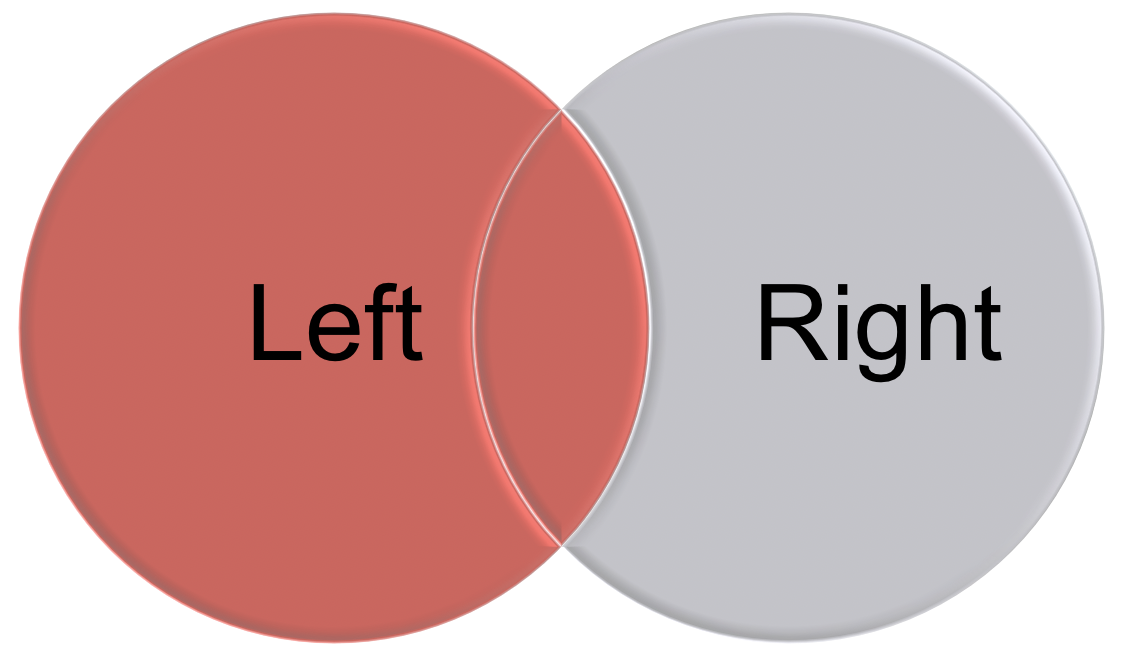
\includegraphics[width=0.3\linewidth]{figures/Left} 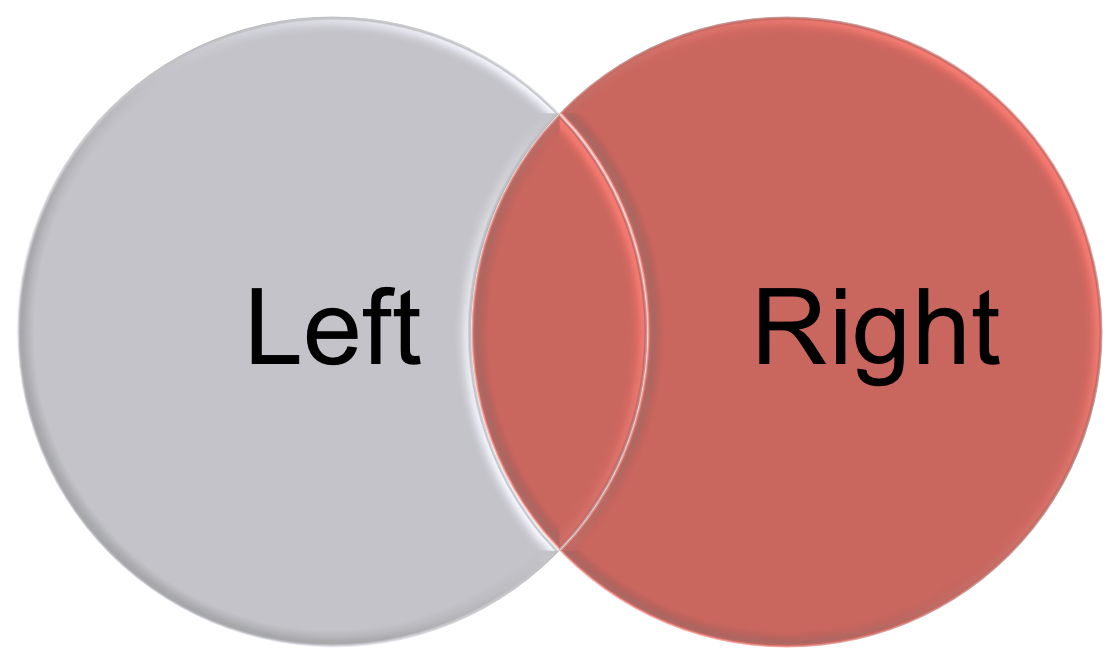
\includegraphics[width=0.3\linewidth]{figures/Right} 

}

\caption{An illustration of left join and right join.}\label{fig:lrjoin}
\end{figure}

Different join functions control what happens to rows that exist in one
table but not the other.

\begin{itemize}
\tightlist
\item
  \texttt{left\_join} keeps all the entries that are present in the left
  (first) table and excludes any that are only in the right table.
\item
  \texttt{right\_join} keeps all the entries that are present in the
  right table and excludes any that are only in the left table.
\item
  \texttt{inner\_join} keeps only the entries that are present in both
  tables. \texttt{inner\_join} is the only function that guarantees you
  won't generate any missing entries.
\item
  \texttt{full\_join} keeps all of the entries in both tables,
  regardless of whether or not they appear in the other table.
\end{itemize}

\begin{figure}

{\centering 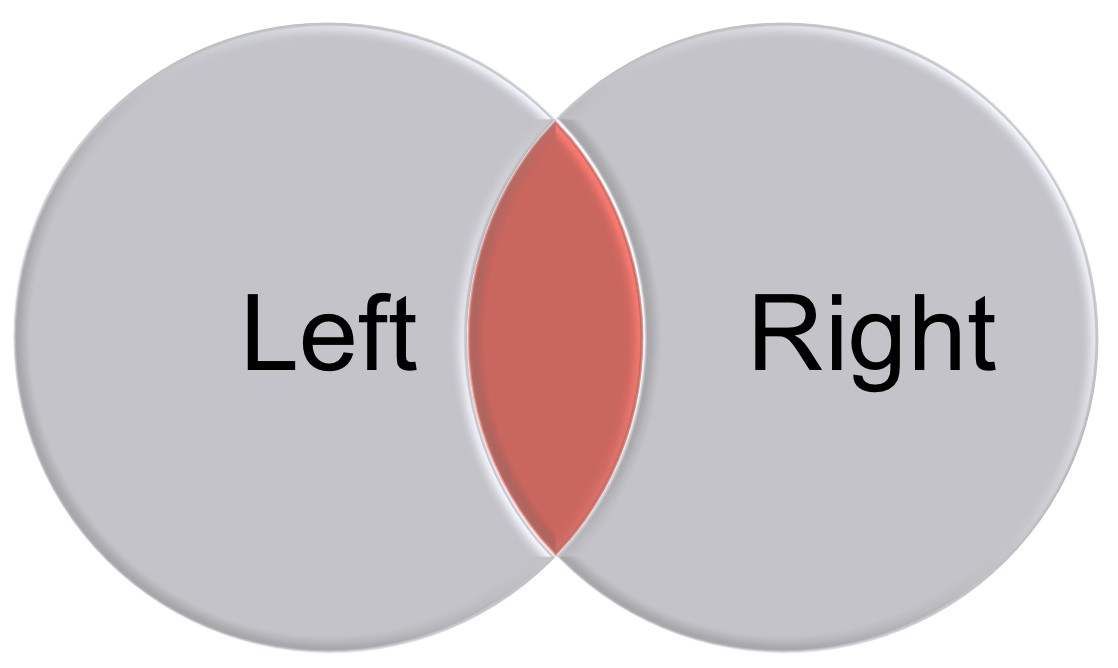
\includegraphics[width=0.3\linewidth]{figures/Inner} 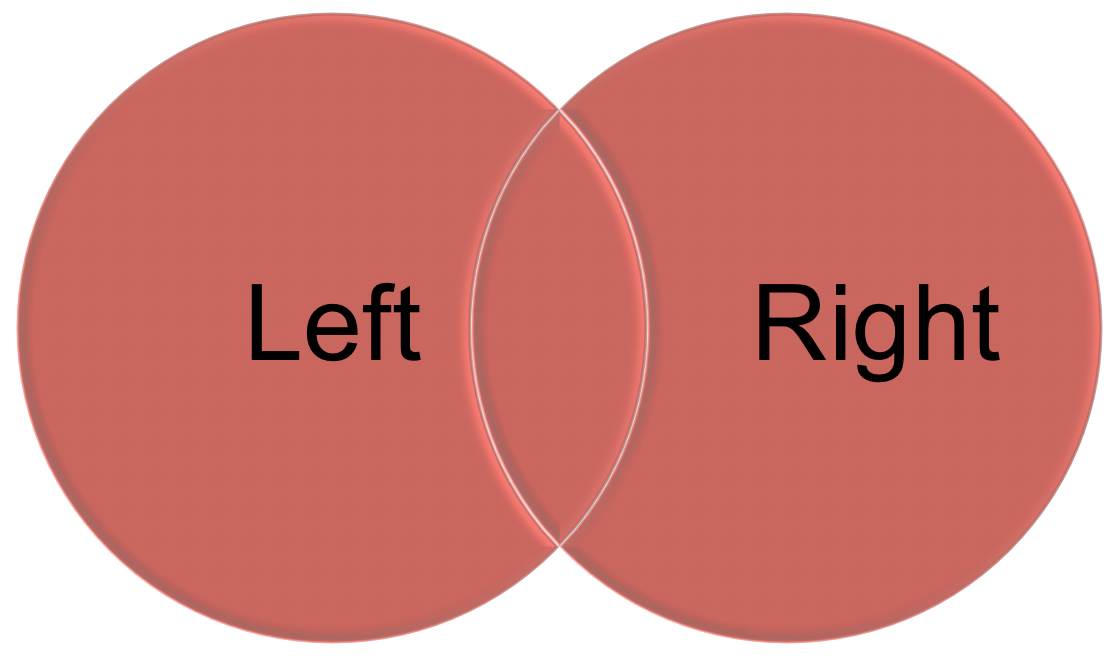
\includegraphics[width=0.3\linewidth]{figures/Full} 

}

\caption{An illustration of inner join and full join.}\label{fig:ifjoin}
\end{figure}

The join functions are nicely illustrated in RStudio's
\href{https://www.rstudio.com/wp-content/uploads/2015/02/data-wrangling-cheatsheet.pdf}{Data
wrangling cheatsheet}.

\begin{figure}

{\centering 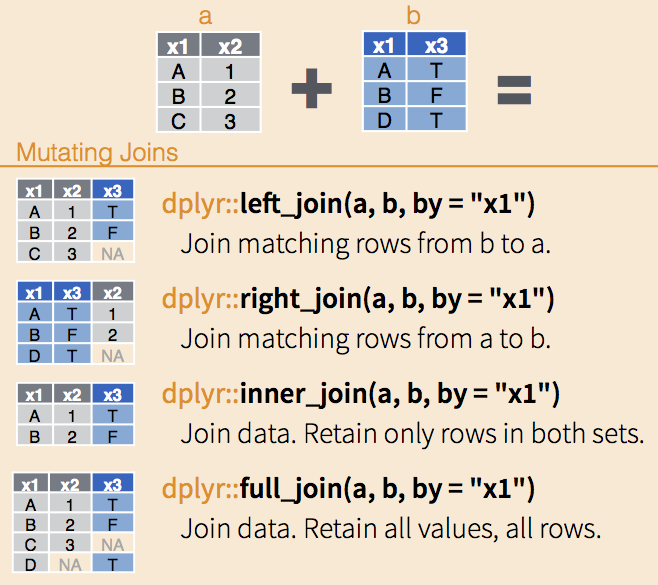
\includegraphics[width=0.75\linewidth]{figures/dplyr-joins} 

}

\caption{An illustration of the join functions in RStudio’s Data wrangling cheatsheet.}\label{fig:join}
\end{figure}

\subsection{Toy examples with joins}\label{toy-examples-with-joins}

\begin{Shaded}
\begin{Highlighting}[]
\NormalTok{a <-}\StringTok{ }\KeywordTok{tibble}\NormalTok{(}\DataTypeTok{x1 =}\NormalTok{ LETTERS[}\KeywordTok{c}\NormalTok{(}\DecValTok{1}\OperatorTok{:}\DecValTok{3}\NormalTok{)], }
                \DataTypeTok{x2 =} \DecValTok{1}\OperatorTok{:}\DecValTok{3}\NormalTok{)}
\NormalTok{b <-}\StringTok{ }\KeywordTok{tibble}\NormalTok{(}\DataTypeTok{x1 =}\NormalTok{ LETTERS[}\KeywordTok{c}\NormalTok{(}\DecValTok{1}\NormalTok{, }\DecValTok{2}\NormalTok{, }\DecValTok{4}\NormalTok{)], }
                \DataTypeTok{x3 =} \KeywordTok{c}\NormalTok{(T, F, T))}
\NormalTok{a}
\NormalTok{## # A tibble: 3 x 2}
\NormalTok{##   x1       x2}
\NormalTok{##   <chr> <int>}
\NormalTok{## 1 A         1}
\NormalTok{## 2 B         2}
\NormalTok{## 3 C         3}
\NormalTok{b}
\NormalTok{## # A tibble: 3 x 2}
\NormalTok{##   x1    x3   }
\NormalTok{##   <chr> <lgl>}
\NormalTok{## 1 A     TRUE }
\NormalTok{## 2 B     FALSE}
\NormalTok{## 3 D     TRUE}
\end{Highlighting}
\end{Shaded}

\begin{Shaded}
\begin{Highlighting}[]
\CommentTok{# include all rows in a and b}
\KeywordTok{inner_join}\NormalTok{(a, b, }\DataTypeTok{by =} \StringTok{"x1"}\NormalTok{)}
\NormalTok{## # A tibble: 2 x 3}
\NormalTok{##   x1       x2 x3   }
\NormalTok{##   <chr> <int> <lgl>}
\NormalTok{## 1 A         1 TRUE }
\NormalTok{## 2 B         2 FALSE}
\end{Highlighting}
\end{Shaded}

\begin{Shaded}
\begin{Highlighting}[]
\CommentTok{# return all rows from a}
\KeywordTok{left_join}\NormalTok{(a, b, }\DataTypeTok{by =} \StringTok{"x1"}\NormalTok{)}
\NormalTok{## # A tibble: 3 x 3}
\NormalTok{##   x1       x2 x3   }
\NormalTok{##   <chr> <int> <lgl>}
\NormalTok{## 1 A         1 TRUE }
\NormalTok{## 2 B         2 FALSE}
\NormalTok{## 3 C         3 NA}
\end{Highlighting}
\end{Shaded}

\begin{Shaded}
\begin{Highlighting}[]
\CommentTok{# return all rows from b}
\KeywordTok{right_join}\NormalTok{(a, b, }\DataTypeTok{by =} \StringTok{"x1"}\NormalTok{)}
\NormalTok{## # A tibble: 3 x 3}
\NormalTok{##   x1       x2 x3   }
\NormalTok{##   <chr> <int> <lgl>}
\NormalTok{## 1 A         1 TRUE }
\NormalTok{## 2 B         2 FALSE}
\NormalTok{## 3 D        NA TRUE}
\end{Highlighting}
\end{Shaded}

\begin{Shaded}
\begin{Highlighting}[]
\CommentTok{# includes all rows in a or b}
\KeywordTok{full_join}\NormalTok{(a, b, }\DataTypeTok{by =} \StringTok{"x1"}\NormalTok{)}
\NormalTok{## # A tibble: 4 x 3}
\NormalTok{##   x1       x2 x3   }
\NormalTok{##   <chr> <int> <lgl>}
\NormalTok{## 1 A         1 TRUE }
\NormalTok{## 2 B         2 FALSE}
\NormalTok{## 3 C         3 NA   }
\NormalTok{## 4 D        NA TRUE}
\end{Highlighting}
\end{Shaded}

\begin{Shaded}
\begin{Highlighting}[]
\CommentTok{# include the rows in a that are not in b}
\KeywordTok{anti_join}\NormalTok{(a, b, }\DataTypeTok{by =} \StringTok{"x1"}\NormalTok{)}
\NormalTok{## # A tibble: 1 x 2}
\NormalTok{##   x1       x2}
\NormalTok{##   <chr> <int>}
\NormalTok{## 1 C         3}
\end{Highlighting}
\end{Shaded}

\begin{Shaded}
\begin{Highlighting}[]
\CommentTok{# want everything that doesn't match?}
\KeywordTok{full_join}\NormalTok{(}\KeywordTok{anti_join}\NormalTok{(a, b, }\DataTypeTok{by =} \StringTok{"x1"}\NormalTok{), }
\KeywordTok{anti_join}\NormalTok{(b, a, }\DataTypeTok{by =} \StringTok{"x1"}\NormalTok{), }\DataTypeTok{by =} \StringTok{"x1"}\NormalTok{)}
\NormalTok{## # A tibble: 2 x 3}
\NormalTok{##   x1       x2 x3   }
\NormalTok{##   <chr> <int> <lgl>}
\NormalTok{## 1 C         3 NA   }
\NormalTok{## 2 D        NA TRUE}
\end{Highlighting}
\end{Shaded}

\subsection{Practice with joins for real
data}\label{practice-with-joins-for-real-data}

\begin{enumerate}
\def\labelenumi{\arabic{enumi}.}
\tightlist
\item
  Example 1
\end{enumerate}

We first get the data named \texttt{pop.county} from the github R
package \texttt{slid}. Note that there are four variables in this data:
``ID'' (county-level Federal Information Processing System code),
``County'' (name of county matched with ``ID''), ``State'' (name of
state matched with ``ID''), \texttt{population} (population of county
matched with ``ID'').

\begin{Shaded}
\begin{Highlighting}[]
\KeywordTok{data}\NormalTok{(I.county)}
\KeywordTok{data}\NormalTok{(pop.county)}
\CommentTok{# make I.county a tibble with as_tibble()}
\NormalTok{I.county <-}\StringTok{ }\KeywordTok{as_tibble}\NormalTok{(I.county)}
\KeywordTok{dim}\NormalTok{(I.county)}
\NormalTok{## [1] 3104  328}
\CommentTok{# make pop.county a tibble with as_tibble()}
\NormalTok{pop.county <-}\StringTok{ }\KeywordTok{as_tibble}\NormalTok{(pop.county)}
\KeywordTok{dim}\NormalTok{(pop.county)}
\NormalTok{## [1] 3142    4}
\end{Highlighting}
\end{Shaded}

Now, we would like to join the two tables: \texttt{I.county} and
\texttt{pop.county} using the \texttt{left\_join} as follows:

\begin{Shaded}
\begin{Highlighting}[]
\NormalTok{pop.county.tmp <-}\StringTok{ }\NormalTok{pop.county }\OperatorTok\StringTok{ }\NormalTok{dplyr}\OperatorTok{::}\KeywordTok{select}\NormalTok{(}\OperatorTok{-}\KeywordTok{c}\NormalTok{(County, State)) }
\NormalTok{I.county.w.pop <-}\StringTok{ }\KeywordTok{left_join}\NormalTok{(I.county, pop.county.tmp, }\DataTypeTok{by =} \StringTok{"ID"}\NormalTok{)}
\end{Highlighting}
\end{Shaded}

or we can:

\begin{Shaded}
\begin{Highlighting}[]
\NormalTok{I.county.w.pop <-}\StringTok{ }\KeywordTok{left_join}\NormalTok{(I.county, }
\NormalTok{dplyr}\OperatorTok{::}\KeywordTok{select}\NormalTok{(pop.county, }\KeywordTok{c}\NormalTok{(ID, population)), }\DataTypeTok{by =} \StringTok{"ID"}\NormalTok{)}
\end{Highlighting}
\end{Shaded}

\begin{enumerate}
\def\labelenumi{\arabic{enumi}.}
\setcounter{enumi}{1}
\tightlist
\item
  Example 2
\end{enumerate}

In this example, we would like to create a map to show the risk of
COVID-19 infection in each state of the US. So, first, we need to have a
new dataset that contains infection risk and the geographic information
of each state. We will get infected count and state population in the
\texttt{state.long} dataset in the \texttt{slid} package.
\texttt{state.long} is a tibble with 15,925 rows and 7 columns. Next, we
obtain the boundary information of each state downloaded from
\href{https://raw.githubusercontent.com/PublicaMundi/MappingAPI/master/data/geojson/us-states.json}{PublicaMundi}.
Then, we merge the two datasets to create a new dataset. We need the R
package \texttt{geojsonio} to read the data from
\href{https://raw.githubusercontent.com/PublicaMundi/MappingAPI/master/data/geojson/us-states.json}{PublicaMundi}.

\begin{Shaded}
\begin{Highlighting}[]
\KeywordTok{library}\NormalTok{(geojsonio)}
\end{Highlighting}
\end{Shaded}

\begin{verbatim}
## Registered S3 method overwritten by 'geojsonsf':
##   method        from   
##   print.geojson geojson
\end{verbatim}

\begin{verbatim}
## 
## Attaching package: 'geojsonio'
\end{verbatim}

\begin{verbatim}
## The following object is masked from 'package:base':
## 
##     pretty
\end{verbatim}

\begin{Shaded}
\begin{Highlighting}[]
\KeywordTok{library}\NormalTok{(slid)}
\KeywordTok{data}\NormalTok{(state.long)}
\CommentTok{# get the geospatial information from PublicaMundi}
\NormalTok{states0 <-}\StringTok{ }\KeywordTok{geojson_read}\NormalTok{(}
  \DataTypeTok{x =} \StringTok{"https://raw.githubusercontent.com/PublicaMundi/MappingAPI/master/data/geojson/us-states.json"}
\NormalTok{  , }\DataTypeTok{what =} \StringTok{"sp"}
\NormalTok{)}
\KeywordTok{head}\NormalTok{(states0}\OperatorTok{@}\NormalTok{data)}
\end{Highlighting}
\end{Shaded}

\begin{verbatim}
##   id       name density
## 1 01    Alabama  94.650
## 2 02     Alaska   1.264
## 3 04    Arizona  57.050
## 4 05   Arkansas  56.430
## 5 06 California 241.700
## 6 08   Colorado  49.330
\end{verbatim}

\begin{Shaded}
\begin{Highlighting}[]
\NormalTok{states1 <-}\StringTok{ }\NormalTok{states0}
\NormalTok{states1}\OperatorTok{@}\NormalTok{data <-}\StringTok{ }\NormalTok{states0}\OperatorTok{@}\NormalTok{data }\OperatorTok\StringTok{ }
\CommentTok{# remove the space in the name of state if there is one}
\KeywordTok{mutate}\NormalTok{(}\DataTypeTok{name_ns =} \KeywordTok{sapply}\NormalTok{(name, gsub, }\DataTypeTok{pattern =} \StringTok{" "}\NormalTok{, }\DataTypeTok{replacement =} \StringTok{""}\NormalTok{))}
\CommentTok{# the following merge step can be done both using sp::merge }
\CommentTok{# or the join functions in dplyr}
\CommentTok{# states1 <- sp::merge(states1, state.long %>% }
\CommentTok{# filter(DATE == as.Date('2020-12-11')), }
\CommentTok{# by.x = "name_ns", by.y = "State")}
\CommentTok{# merge the two datasets}
\NormalTok{states1}\OperatorTok{@}\NormalTok{data <-}\StringTok{ }\KeywordTok{left_join}\NormalTok{(states1}\OperatorTok{@}\NormalTok{data, state.long }\OperatorTok\StringTok{ }
\KeywordTok{filter}\NormalTok{(DATE }\OperatorTok{==}\StringTok{ }\KeywordTok{as.Date}\NormalTok{(}\StringTok{'2020-12-11'}\NormalTok{)), }
\DataTypeTok{by =} \KeywordTok{c}\NormalTok{(}\StringTok{'name_ns'}\NormalTok{ =}\StringTok{ 'State'}\NormalTok{))}
\CommentTok{# calculate the risk of infection}
\NormalTok{states1}\OperatorTok{@}\NormalTok{data <-}\StringTok{ }\NormalTok{states1}\OperatorTok{@}\NormalTok{data }\OperatorTok\StringTok{ }
\StringTok{  }\KeywordTok{mutate}\NormalTok{(}\DataTypeTok{Infect_risk =}\NormalTok{ Infected }\OperatorTok{/}\StringTok{ }\NormalTok{pop)}
\end{Highlighting}
\end{Shaded}

\section{Reshaping Data}\label{reshaping-data}

Sometimes, we want to convert data from a wide format to a long format.
Many functions in R expect data to be in a long format rather than a
wide format. Programs like SPSS, however, often use wide-formatted data.
Take the dataset I.state for example, the column names ``XYYYY.MM.DD''
are not names of variables, but values of a variable, which contains the
values of cumulative infected count.\\
We need to pivot the column names into new variables.

There are two sets of methods that are explained below:

\begin{itemize}
\item
  \texttt{gather()} and \texttt{spread()} from the \texttt{tidyr}
  package. This is a newer interface to the \texttt{reshape2} package.
\item
  \texttt{pivot\_longer} and \texttt{pivot\_wider} from the
  \texttt{tidyr} package.
\end{itemize}

Many other methods aren't covered here since they are not as easy to
use.

\subsection{From wide to long}\label{from-wide-to-long}

Below we would like to change the data \texttt{I.state} from wide format
to long format.

\begin{Shaded}
\begin{Highlighting}[]
\KeywordTok{library}\NormalTok{(slid)}
\KeywordTok{data}\NormalTok{(I.state)}
\KeywordTok{names}\NormalTok{(I.state)}
\end{Highlighting}
\end{Shaded}

\begin{enumerate}
\def\labelenumi{\arabic{enumi}.}
\tightlist
\item
  Use \texttt{gather(data,\ key,\ value,\ ...)}
\end{enumerate}

\begin{itemize}
\tightlist
\item
  \texttt{data} = the dataframe you want to morph from wide to long
\item
  \texttt{key} = the name of the new column that is levels of what is
  represented in the wide format as many columns
\item
  \texttt{value} = the name of the column that will contain the values
\item
  \texttt{...} = columns to gather, or leave (use -column to gather all
  except that one)
\end{itemize}

The \texttt{gather} functions are nicely illustrated in RStudio's
{[}Data wrangling
cheatsheet{]}{[}\url{https://rstudio.com/wp-content/uploads/2015/02/data-wrangling-cheatsheet.pdf}{]}
as shown in Figure \ref{fig:gather}.

\begin{figure}

{\centering 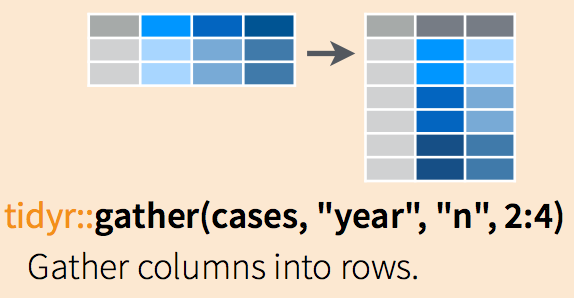
\includegraphics[width=0.5\linewidth]{figures/gather} 

}

\caption{An illustration of `gather` function.}\label{fig:gather}
\end{figure}

\begin{Shaded}
\begin{Highlighting}[]
\CommentTok{# method 1}
\NormalTok{I.state.wide <-}\StringTok{ }\NormalTok{I.state }
\KeywordTok{dim}\NormalTok{(I.state.wide)  }
\end{Highlighting}
\end{Shaded}

\begin{verbatim}
## [1]  49 326
\end{verbatim}

\begin{Shaded}
\begin{Highlighting}[]
\NormalTok{I.state.long <-}\StringTok{ }\KeywordTok{gather}\NormalTok{(I.state.wide, DATE, Infected, }
\NormalTok{X2020.}\FloatTok{12.11}\OperatorTok{:}\NormalTok{X2020.}\FloatTok{01.22}\NormalTok{, }\DataTypeTok{factor_key =} \OtherTok{TRUE}\NormalTok{) }\OperatorTok\StringTok{ }
\StringTok{                       }\KeywordTok{arrange}\NormalTok{(State)}
\KeywordTok{dim}\NormalTok{(I.state.long)}
\end{Highlighting}
\end{Shaded}

\begin{verbatim}
## [1] 15925     3
\end{verbatim}

\begin{enumerate}
\def\labelenumi{\arabic{enumi}.}
\setcounter{enumi}{1}
\tightlist
\item
  Use \texttt{pivot\_longer()}
\end{enumerate}

The function \texttt{pivot\_longer()} is an updated approach to
\texttt{gather()}, designed to be both simpler to use and to handle more
use cases. It is recommended to use \texttt{pivot\_longer()} for new
code; \texttt{gather()} isn't going away but is no longer under active
development.

\begin{Shaded}
\begin{Highlighting}[]
\CommentTok{# method 2}
\NormalTok{I.state.wide <-}\StringTok{ }\NormalTok{I.state }
\KeywordTok{dim}\NormalTok{(I.state.wide) }
\end{Highlighting}
\end{Shaded}

\begin{verbatim}
## [1]  49 326
\end{verbatim}

\begin{Shaded}
\begin{Highlighting}[]
\NormalTok{I.state.long <-}\StringTok{ }\NormalTok{I.state.wide }\OperatorTok
\StringTok{  }\KeywordTok{pivot_longer}\NormalTok{(X2020.}\FloatTok{12.11}\OperatorTok{:}\NormalTok{X2020.}\FloatTok{01.22}\NormalTok{, }\DataTypeTok{names_to =} \StringTok{"DATE"}\NormalTok{, }
  \DataTypeTok{values_to =} \StringTok{"Infected"}\NormalTok{)}
\end{Highlighting}
\end{Shaded}

See more complicated examples from the
\href{https://tidyr.tidyverse.org/reference/pivot_longer.html}{introduction
of `tidyr' package}.

\subsection{From long to wide}\label{from-long-to-wide}

Now let's change the data back to the wide format, and we can use
\texttt{spread}.

\begin{enumerate}
\def\labelenumi{\arabic{enumi}.}
\tightlist
\item
  Use \texttt{Use\ spread(data,\ key,\ value)}
\end{enumerate}

\begin{itemize}
\tightlist
\item
  \texttt{data} = the dataframe you want to morph from long to wide
\item
  \texttt{key} = the name of the column that contains the key
\item
  \texttt{value} = the name of the column contains the values
\end{itemize}

The \texttt{spread} functions are nicely illustrated in RStudio's
{[}Data wrangling
cheatsheet{]}{[}\url{https://rstudio.com/wp-content/uploads/2015/02/data-wrangling-cheatsheet.pdf}{]}
as shown in Figure \ref{fig:spread}.

\begin{figure}

{\centering 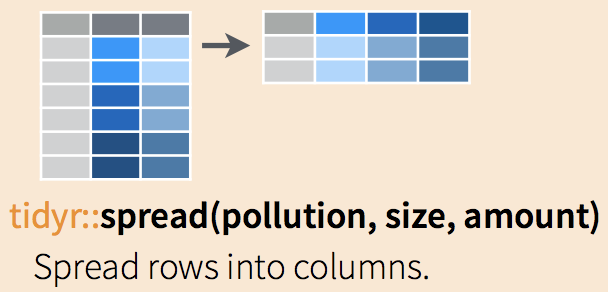
\includegraphics[width=0.5\linewidth]{figures/spread} 

}

\caption{An illustration of `spread` function.}\label{fig:spread}
\end{figure}

\begin{Shaded}
\begin{Highlighting}[]
\CommentTok{# method 1}
\NormalTok{I.state.wide <-}\StringTok{ }\KeywordTok{spread}\NormalTok{(I.state.long, DATE, Infected)}
\KeywordTok{dim}\NormalTok{(I.state.wide)}
\end{Highlighting}
\end{Shaded}

\begin{verbatim}
## [1]  49 326
\end{verbatim}

\begin{enumerate}
\def\labelenumi{\arabic{enumi}.}
\setcounter{enumi}{1}
\tightlist
\item
  Use \texttt{pivot\_wider()}
\end{enumerate}

We can also use the function \texttt{pivot\_wider()}, which ``widens''
data, increasing the number of columns and decreasing the number of
rows. The inverse transformation is \texttt{pivot\_longer()}.

\begin{Shaded}
\begin{Highlighting}[]
\CommentTok{# method 2}
\NormalTok{I.state.wide <-}\StringTok{ }\NormalTok{I.state.long }\OperatorTok
\KeywordTok{pivot_wider}\NormalTok{(}\DataTypeTok{names_from =}\NormalTok{ DATE, }\DataTypeTok{values_from =}\NormalTok{ Infected)}
\KeywordTok{dim}\NormalTok{(I.state.wide)}
\end{Highlighting}
\end{Shaded}

\begin{verbatim}
## [1]  49 326
\end{verbatim}

See more complicated examples from the
\href{https://tidyr.tidyverse.org/reference/pivot_longer.html}{introduction
of `tidyr' package}.

\section{Exercises}\label{exercises}

\begin{enumerate}
\def\labelenumi{\arabic{enumi}.}
\tightlist
\item
  We are going to explore the basic data manipulation verbs of
  \texttt{dplyr} using \texttt{I.county}. Install the github R package
  \texttt{slid}.
\end{enumerate}

\begin{Shaded}
\begin{Highlighting}[]
\KeywordTok{library}\NormalTok{(slid)}
\KeywordTok{data}\NormalTok{(I.county)}
\end{Highlighting}
\end{Shaded}

\begin{enumerate}
\def\labelenumi{(\alph{enumi})}
\item
  Obtain a subset of the \texttt{I.county} by selecting \texttt{ID},
  \texttt{County}, \texttt{State}.
\item
  Obtain a subset of the \texttt{I.county} by including all counties in
  California.
\item
  Obtain a subset of the \texttt{I.county} by including all counties
  that in the midwest states.
\end{enumerate}

\begin{Shaded}
\begin{Highlighting}[]
\NormalTok{Midwest  =}\StringTok{ }\KeywordTok{c}\NormalTok{( }\StringTok{"Illinois"}\NormalTok{, }\StringTok{"Michigan"}\NormalTok{, }\StringTok{"Indiana"}\NormalTok{ ,}\StringTok{"Ohio"}\NormalTok{, }
\StringTok{"Wisconsin"}\NormalTok{, }\StringTok{"Iowa"}\NormalTok{, }\StringTok{"Kansas"}\NormalTok{, }\StringTok{"Minnesota"}\NormalTok{, }\StringTok{"Missouri"}\NormalTok{, }
\StringTok{"Nebraska"}\NormalTok{ , }\StringTok{"SouthDakota"}\NormalTok{ , }\StringTok{"NorthDakota"}\NormalTok{)}
\end{Highlighting}
\end{Shaded}

\begin{enumerate}
\def\labelenumi{(\alph{enumi})}
\setcounter{enumi}{3}
\item
  Obtain a subset of the \texttt{I.county} by including the top ten
  counties from each midwest state based on the cumulative infected
  count on December 11, 2020.
\item
  Obtain a subset of the \texttt{I.county} by including all the counties
  California with the culumative infected counts up till Judy 31, 2020.
\item
  Create new columns of \texttt{I.county} by taking the logarithm of
  each of the count column.
\item
  Sort the cumulative infected count on December 11, 2020 to find the
  state with the largest cumulative infected count.
\end{enumerate}

\begin{enumerate}
\def\labelenumi{\arabic{enumi}.}
\setcounter{enumi}{1}
\tightlist
\item
  Downlad the data \texttt{pop.county} from the github R package
  \texttt{slid}.
\end{enumerate}

\begin{enumerate}
\def\labelenumi{(\alph{enumi})}
\item
  Join the tables of \texttt{I.county} and \texttt{pop.county} using
  \texttt{inner\_join}, \texttt{left\_join} , \texttt{right\_join},
  \texttt{full\_join}. Do you get same or different tables?
\item
  Based on the \texttt{inner\_join} create a table and name it as
  \texttt{I.pop.county}, then create new columns of
  \texttt{I.pop.county} by dividing each of the count column by the
  popolation in the corresponding county, for example,
  \texttt{risk.2020.12.11\ =\ X.2020.12.11\ /\ pop}.
\item
  For each state, list the top ten county with the highest risk based on
  \texttt{risk.2020.12.11}
\end{enumerate}

\chapter{Data Visualization with ggplot2}\label{ggplot2}

\section{Introduction}\label{introduction}

The first thing to do in the epidemiologic data analysis task is to plot
the data. Data visualization enables many features of the data to be
displayed or summarized in a graphical format, including patterns,
unusual observations, changes over time, spatial variations, and
relationships among variables. The features that are seen in graphs of
the data must then be incorporated, as much as possible, into the
modeling or forecasting methods.

There are many types of graphs available, each with its own strengths
and use cases. One of the challenges in the statistical learning process
is choosing the appropriate visualization method to represent the data.
Before constructing any display of epidemiologic data, it is important
to understand the type of task that we want to perform and determine the
information to convey. Some common roles for data visualization include:

\begin{itemize}
\tightlist
\item
  highlighting a change from past patterns in the data;
\item
  displaying a part-to-whole composition;
\item
  showing how data is distributed;
\item
  showing a difference or similarity between groups;
\item
  displaying the spatial variation in geographical data;
\item
  illustrating relationships among variables.
\end{itemize}

When the data are more complex, graphs can help visualize broader
patterns and trends and identify variations from those trends.
Variations in data may represent important new findings or only errors
in typing or coding which need to be corrected. Thus, graphs can be
helpful tools to aid in verifying and analyzing the data. Once an
analysis is complete, graphs further serve as useful visual aids for
describing the data to others.

This chapter will introduce the \texttt{ggplot2}, and we will gain
insight and practical skills for visualization of infectious disease
data.

Recommended Reading:

\begin{enumerate}
\def\labelenumi{\arabic{enumi}.}
\tightlist
\item
  \url{https://ggplot2.tidyverse.org}
\item
  \url{https://opr.princeton.edu/workshops/Downloads/}
\item
  \url{https://ggplot2-book.org/introduction.html}
\end{enumerate}

\texttt{ggplot2} builds on
\href{https://stanford.idm.oclc.org/login?url=http://www.myilibrary.com?id=46066}{Leland
Wilkinson's The Grammar of Graphics} and focuses on the primacy of
layers and adapts it for R.

\begin{quote}
In brief, the grammar tells us that a graphic maps the data to the
aesthetic attributes (color, shape, size) of geometric objects (points,
lines, bars). The plot may also include statistical transformations of
the data and information about the plot's coordinate system. Facetting
can be used to plot for different subsets of the data. The combination
of these independent components is what makes up a graphic.
\end{quote}

In this chapter, we will introduce the basics of \texttt{ggplot2}
grammar and some of the key features, including the use of
\texttt{geom}, \texttt{stat}, \texttt{scale}, \texttt{coord}, and
\texttt{facet}.

\section{Types of Variables and
Preparation}\label{types-of-variables-and-preparation}

When preparing graphs, keep in mind that the primary purpose is to
communicate information. The types of variables we are analyzing and the
media for the visualization can also affect your graphics practice.

\subsection{Types of Variables}\label{types-of-variables}

In examining data, you must know which data type you are dealing with to
choose the appropriate display format. The data are ususally in one of
the following categories:

\begin{enumerate}
\def\labelenumi{\arabic{enumi}.}
\tightlist
\item
  Categorical (Qualitative) variables
\end{enumerate}

\begin{itemize}
\item
  A \textbf{nominal} variable is one whose values are categories without
  any numerical ranking. Good examples are occupation, place of birth,
  county of residence and diagnosis. Nominal variable is called
  \textbf{dichotomous} when it is characterised by only two classes. In
  epidemiology, it is common to see dichotomous variables: sex
  (male/female), exposure history (yes/no), alive or dead, ill or well,
  vaccinated or unvaccinated.
\item
  An \textbf{ordinale} variable has values that can be ranked but are
  not necessarily evenly spaced. For example, severity of illness may be
  categorised and ordered as ``mild'', ``moderate'' or ``severe''.
\end{itemize}

\begin{enumerate}
\def\labelenumi{\arabic{enumi}.}
\setcounter{enumi}{1}
\tightlist
\item
  Numerical (Quantitative) variables
\end{enumerate}

There are two types of \textbf{quantitative} variables:

\begin{itemize}
\item
  \textbf{Discrete} variables have values that are distinct and
  separate. Discrete data can't be measured but can be counted. For
  example, the number of new cases of a certain disease in a given year.
\item
  \textbf{Continuous} variables represents measurements and can have any
  value in a range. Examples of continuous data would be the amount of
  the time period between when you catch a virus and when your symptoms
  start. Discrete data can't be counted but can be measured.
\item
  An \textbf{interval-scale} variable is measured on a scale of equally
  spaced units, but without a true zero point. An example of interval
  data is date of birth.
\item
  A \textbf{ratio-scale} variable is the same as interval values, with
  the difference that they do have an absolute zero. Good examples are
  be height in centimeters or duration of illness.
\end{itemize}

\subsection{Rules for Graph Designing}\label{rules-for-graph-designing}

When designing graphs, we need to follow some rules to achieve the best
practices, and \citet{dicker1992principles} suggests the following:

\begin{itemize}
\item
  Ensure that a graphic can stand alone by clear labeling of title,
  source, axes, scales, and legends;
\item
  Clearly identify variables portrayed (legends or keys), including
  units of measure;
\item
  Minimize number of lines on a graph;
\item
  Generally, portray frequency on the vertical scale, starting at zero,
  and classification variable on horizontal scale;
\item
  Ensure that scales for each axis are appropriate for data presented;
\item
  Define any abbreviations or symbols; and
\item
  Specify any data excluded.
\end{itemize}

\subsection{Installing packages and loading
data}\label{installing-packages-and-loading-data}

Before we begin, please get ready by installing the \texttt{ggplot2}
package by any of the following method.

\begin{Shaded}
\begin{Highlighting}[]
\CommentTok{# The easiest way to get ggplot2 is to install the whole tidyverse:}
\KeywordTok{install.packages}\NormalTok{(}\StringTok{"tidyverse"}\NormalTok{)}

\CommentTok{# Alternatively, install just ggplot2:}
\KeywordTok{install.packages}\NormalTok{(}\StringTok{"ggplot2"}\NormalTok{)}

\CommentTok{# Or the development version from GitHub:}
\CommentTok{# install.packages("devtools")}
\NormalTok{devtools}\OperatorTok{::}\KeywordTok{install_github}\NormalTok{(}\StringTok{"tidyverse/ggplot2"}\NormalTok{)}
\end{Highlighting}
\end{Shaded}

\textbf{Note:} \texttt{devtools} downloads and installs the package from
GitHub. By default, \texttt{install.packages()} is only able to install
packages that are available in Comprehensive R Archive Network (CRAN).
In that case, the developer's tool, \texttt{devtools::install\_github()}
enables users to install packages that have not been submitted to CRAN,
but is available in GitHub.

In addition, we need to library the required packages as following.

In the rest of this section, we demonstrate how to create a basic
scatter plot and output the figure in ``png'' and ``rds'' format. To
create a \texttt{ggplot2} plot, we need to know three key components:
(1) A dataframe with each column being an attribute/variable, each row
being an individual; (2) A set of aesthetic mappings between variables
in the data and visual properties, and (3) At least one layer which
describes how to render each observation. Layers are usually created
with a \texttt{geom} function.

``ggplot'' generally likes data in the ``long'' format: i.e., a column
for every dimension, and a row for every observation. For illustration,
we are going to use the \texttt{state.long} dataset in the R package
\texttt{slid}. To prepare the data, install the R package \texttt{slid}
from Github using the following command, which includes the datasets
that we use for this book.

Open the \texttt{state.long} dataset, which includes the variables,
cumulative infected cases (\texttt{Infected}), cumulative death counts
(\texttt{Death}), \texttt{Region}, \texttt{Division}, \texttt{State},
population (\texttt{pop}), and \texttt{DATE}, starting from Jan 22,
2020. Take a look at the first few lines using \texttt{head()}.

\begin{Shaded}
\begin{Highlighting}[]
\NormalTok{df <-}\StringTok{ }\NormalTok{slid}\OperatorTok{::}\NormalTok{state.long}

\KeywordTok{head}\NormalTok{(df)}
\end{Highlighting}
\end{Shaded}

\begin{verbatim}
## # A tibble: 6 x 7
##   State  Region Division       pop DATE       Infected Death
##   <fct>  <fct>  <fct>        <int> <date>        <int> <int>
## 1 Alaba~ South  East South~ 4.89e6 2020-12-11   288775  4086
## 2 Alaba~ South  East South~ 4.89e6 2020-12-10   284922  4034
## 3 Alaba~ South  East South~ 4.89e6 2020-12-09   280187  3985
## 4 Alaba~ South  East South~ 4.89e6 2020-12-08   276665  3940
## 5 Alaba~ South  East South~ 4.89e6 2020-12-07   272228  3891
## 6 Alaba~ South  East South~ 4.89e6 2020-12-06   269877  3888
\end{verbatim}

\subsection{Your first scatterplot}\label{your-first-scatterplot}

Here we introduce how to draw a simple scatter plot using the data of
`2020-12-11'. Treat \texttt{log(Infected)} as the x-axis, and
\texttt{log(Death)} as the y-axis. We create it by telling ``ggplot''
the data \texttt{df}, the aesthetic mapping
\texttt{aes(log(Infected),\ log(Death))}, and the layer
\texttt{geom\_point()}. The structure
\texttt{ggplot()\ +\ geom\_point()} is the typical way to create a plot,
in which ``ggplot'' is told the data and mapping, and
\texttt{geom\_point} is a layer of a picture using the information
embedded in ``ggplot''. Later in this chapter, you will see how we can
use \texttt{+} to assign additional adjustments and add multiple layers
to the existing figure.

\begin{Shaded}
\begin{Highlighting}[]
\CommentTok{# Select the date}
\NormalTok{df <-}\StringTok{ }\NormalTok{slid}\OperatorTok{::}\NormalTok{state.long }\OperatorTok\StringTok{ }
\StringTok{  }\NormalTok{dplyr}\OperatorTok{::}\KeywordTok{filter}\NormalTok{(DATE }\OperatorTok{==}\StringTok{ }\KeywordTok{as.Date}\NormalTok{(}\StringTok{'2020-12-11'}\NormalTok{)) }

\CommentTok{# Create scatter plot}
\CommentTok{# Data: df}
\CommentTok{# Aesthetic: first mapped to x, second mapped to y}
\CommentTok{# Layer: render the plot as a scatterplot}
\NormalTok{p <-}\StringTok{ }\KeywordTok{ggplot}\NormalTok{(df, }\KeywordTok{aes}\NormalTok{(}\KeywordTok{log}\NormalTok{(Infected }\OperatorTok{+}\StringTok{ }\DecValTok{1}\NormalTok{), }\KeywordTok{log}\NormalTok{(Death }\OperatorTok{+}\StringTok{ }\DecValTok{1}\NormalTok{)))}
\NormalTok{p }\OperatorTok{+}\StringTok{ }\KeywordTok{geom_point}\NormalTok{()         }
\end{Highlighting}
\end{Shaded}

\begin{figure}

{\centering 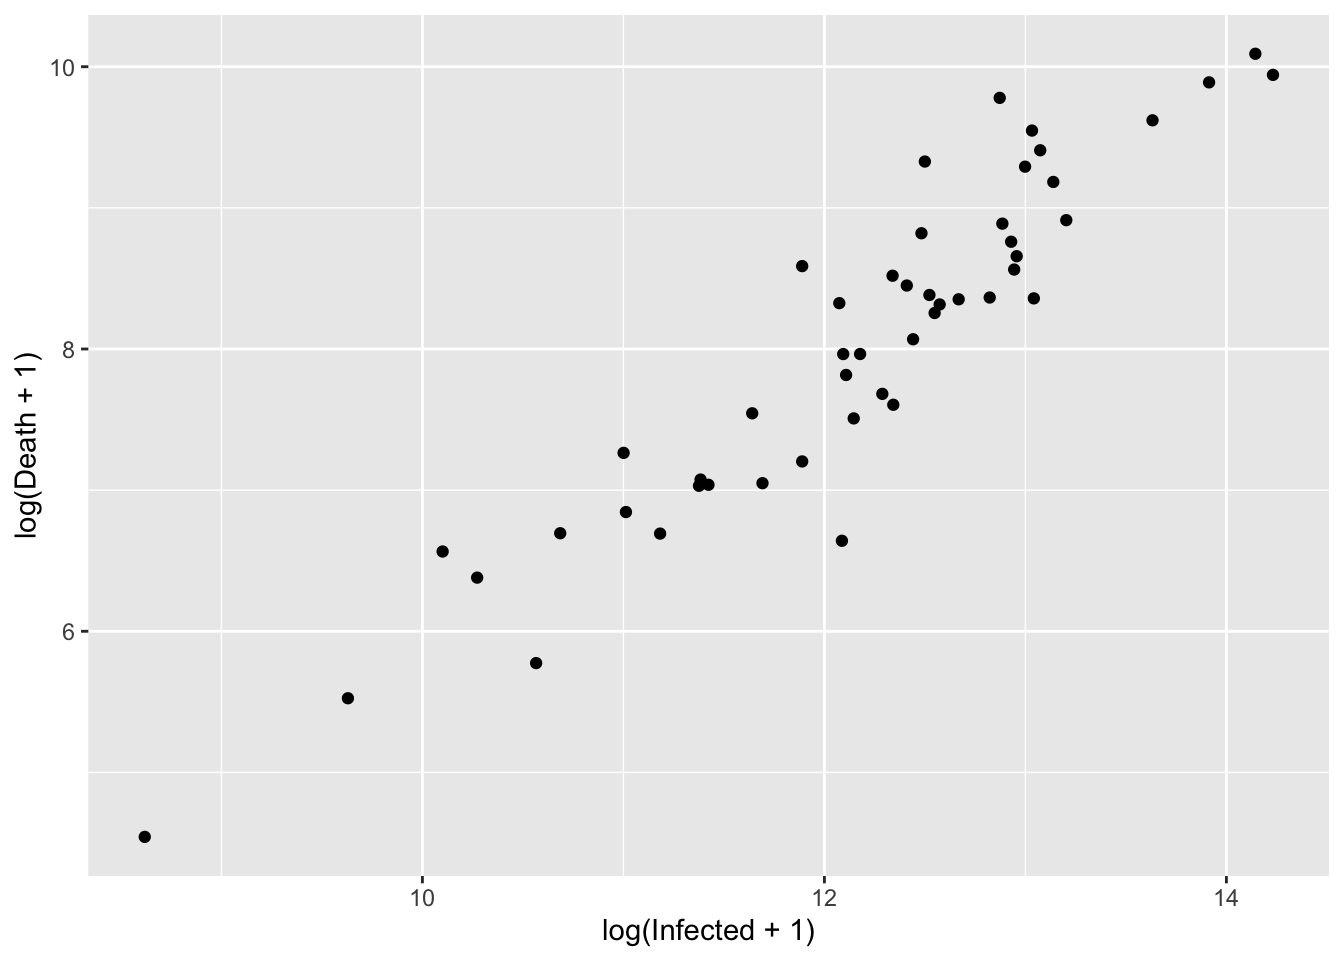
\includegraphics[width=0.5\linewidth]{bookdown-demo_files/figure-latex/ggplotscatter1-1} 

}

\caption{Scatterplot of log cumulative death against log cumulative infected}\label{fig:ggplotscatter1}
\end{figure}

\textbf{Remarks:}

In the above example, the dataframe \texttt{df} is the first parameter
in the above \texttt{ggplot()}, and aesthetics are defined within an
\texttt{aes()} function. We need to place \texttt{+} at the end of the
previous line instead of the beginning of new line.

\textbf{Aesthetics} are properties of the plot that can show certain
elements of the data. The following is a list of some common plot
aesthetics you might want to specify in your \texttt{geom\_point()}:

\begin{itemize}
\tightlist
\item
  \texttt{x}: position on x-axis
\item
  \texttt{y}: position on y-axis
\item
  \texttt{alpha}: transparency (1: opaque; 0: transparent)
\item
  \texttt{color}: color of border of elements
\item
  \texttt{fill}: color of inside of elements
\item
  \texttt{shape}: shape
\item
  \texttt{group}: group
\item
  \texttt{size}: size
\item
  \texttt{stroke}: border size of points
\end{itemize}

We will explain more details in the following sections.

\section{Position Scales and Axes}\label{position-scales-and-axes}

\subsection{\texorpdfstring{Change the labels of the axis using
\texttt{xlab()} and
\texttt{ylab()}}{Change the labels of the axis using xlab() and ylab()}}\label{change-the-labels-of-the-axis-using-xlab-and-ylab}

See Figure \ref{fig:xlabggplot} for the customized labels and title.

\begin{Shaded}
\begin{Highlighting}[]
\CommentTok{# Change the transparency using alpha}
\NormalTok{p <-}\StringTok{ }\NormalTok{p }\OperatorTok{+}\StringTok{ }\KeywordTok{geom_point}\NormalTok{(}\DataTypeTok{alpha =} \FloatTok{0.7}\NormalTok{) }\OperatorTok{+}\StringTok{ }
\StringTok{   }\CommentTok{# Change the label of horizontal axis}
\StringTok{  }\KeywordTok{xlab}\NormalTok{(}\StringTok{'log Infected'}\NormalTok{) }\OperatorTok{+}
\StringTok{  }\CommentTok{# Change the label of vertical axis}
\StringTok{  }\KeywordTok{ylab}\NormalTok{(}\StringTok{'log Death'}\NormalTok{) }\OperatorTok{+}\StringTok{ }
\StringTok{  }\CommentTok{# Change the title}
\StringTok{  }\KeywordTok{labs}\NormalTok{(}\DataTypeTok{title =} \StringTok{'Log death against infected cases in US'}\NormalTok{)}
\NormalTok{p}
\end{Highlighting}
\end{Shaded}

\begin{figure}

{\centering 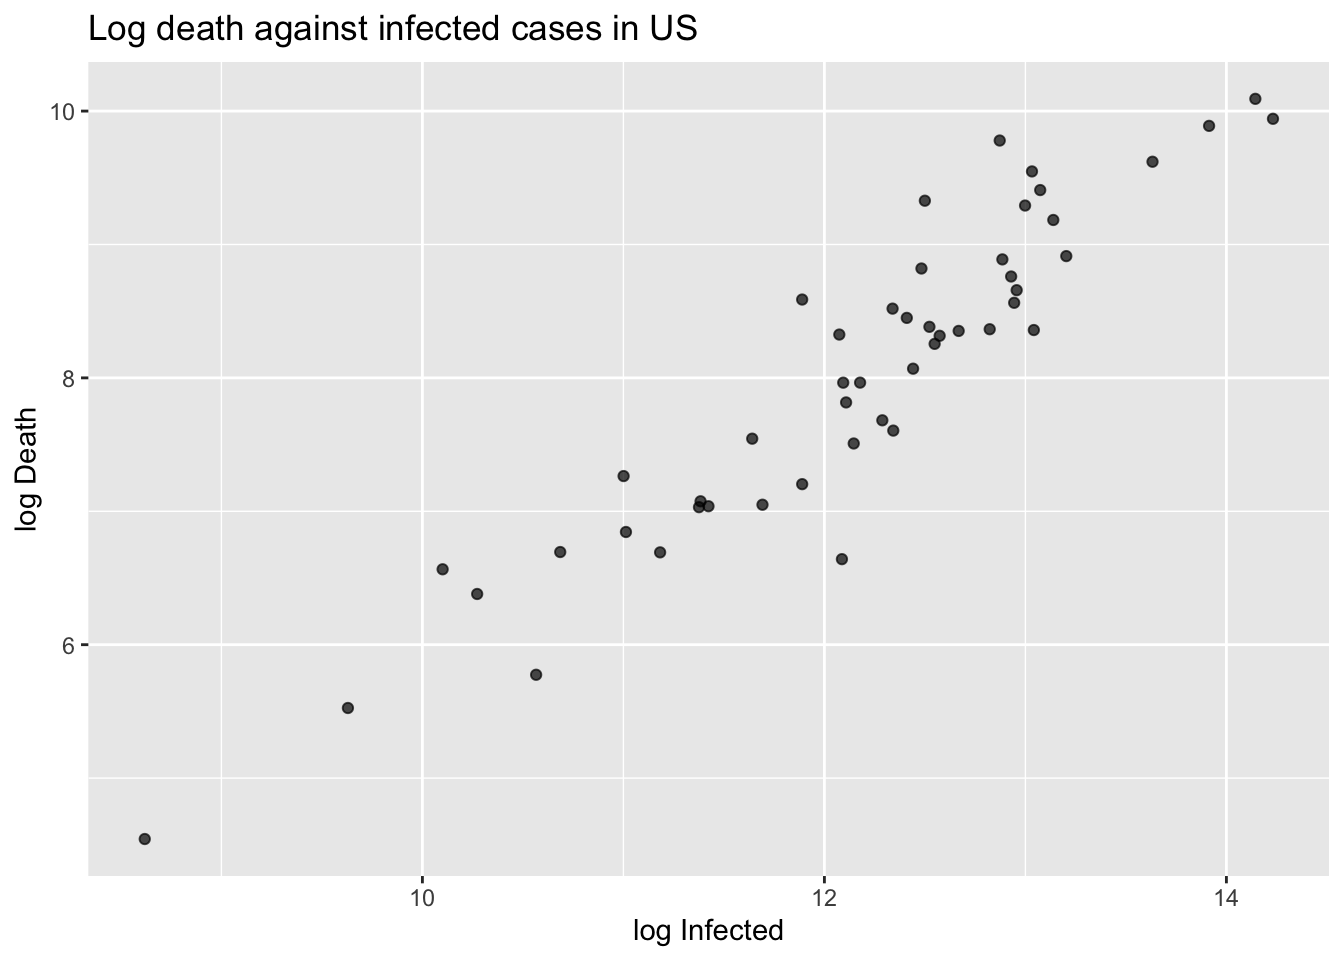
\includegraphics[width=0.5\linewidth]{bookdown-demo_files/figure-latex/xlabggplot-1} 

}

\caption{Scatterplot with customized lables and title}\label{fig:xlabggplot}
\end{figure}

\begin{Shaded}
\begin{Highlighting}[]
\CommentTok{#p + scale_x_reverse()}
\CommentTok{#p + scale_y_reverse()}
\end{Highlighting}
\end{Shaded}

\subsection{\texorpdfstring{Change the range of the axis using
\texttt{xlim()} and
\texttt{ylim()}}{Change the range of the axis using xlim() and ylim()}}\label{change-the-range-of-the-axis-using-xlim-and-ylim}

For continuous variables, we can provide the lower and upper limits. For
categorical variables, we can provide the names of categories desired.
To suppress the warning ``Removed XXX rows containing missing values'',
use \texttt{na.rm}. This needs to be carefully used because the data
outside the range are converted to \texttt{NA}, which will affect later
manipulations, such as calculating the mean or sum.

\begin{Shaded}
\begin{Highlighting}[]
\CommentTok{# For continuous variable, provide the lower and upper limits}
\NormalTok{p <-}\StringTok{ }\NormalTok{p }\OperatorTok{+}\StringTok{ }\KeywordTok{geom_point}\NormalTok{() }\OperatorTok{+}\StringTok{ }\KeywordTok{ylim}\NormalTok{(}\DecValTok{4}\NormalTok{, }\DecValTok{12}\NormalTok{) }
\NormalTok{p}
\end{Highlighting}
\end{Shaded}

\begin{figure}

{\centering 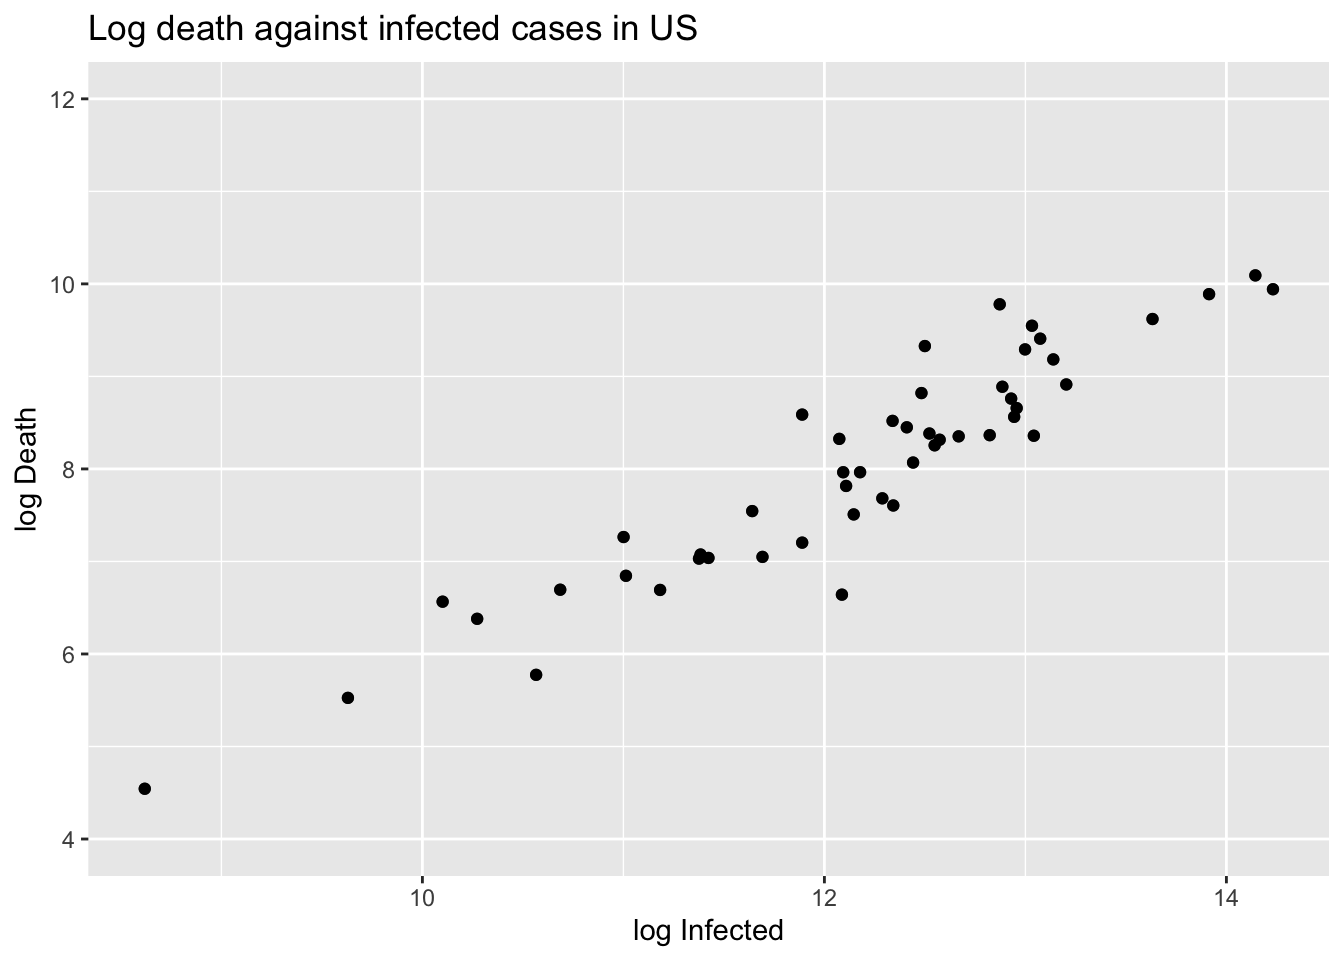
\includegraphics[width=0.5\linewidth]{bookdown-demo_files/figure-latex/xlimggplot-1} 

}

\caption{Scatterplot with customized axis range for continuous features}\label{fig:xlimggplot}
\end{figure}

\begin{Shaded}
\begin{Highlighting}[]
\CommentTok{# For discrete variable, provide the names of categories desired}
\CommentTok{# To suppress the warning 'Removed XXX rows containing...', use `na.rm`. }
\NormalTok{df <-}\StringTok{ }\NormalTok{slid}\OperatorTok{::}\NormalTok{state.long }\OperatorTok\StringTok{ }
\StringTok{  }\NormalTok{dplyr}\OperatorTok{::}\KeywordTok{filter}\NormalTok{(DATE }\OperatorTok{==}\StringTok{ }\KeywordTok{as.Date}\NormalTok{(}\StringTok{'2020-12-11'}\NormalTok{)) }

\KeywordTok{ggplot}\NormalTok{(df, }\KeywordTok{aes}\NormalTok{(Region, }\KeywordTok{log}\NormalTok{(Death }\OperatorTok{+}\StringTok{ }\DecValTok{1}\NormalTok{))) }\OperatorTok{+}\StringTok{ }
\StringTok{  }\KeywordTok{geom_point}\NormalTok{(}\DataTypeTok{na.rm =} \OtherTok{TRUE}\NormalTok{) }\OperatorTok{+}
\StringTok{  }\KeywordTok{xlim}\NormalTok{(}\StringTok{'West'}\NormalTok{, }\StringTok{'Midwest'}\NormalTok{, }\StringTok{'South'}\NormalTok{) }
\end{Highlighting}
\end{Shaded}

\begin{figure}

{\centering 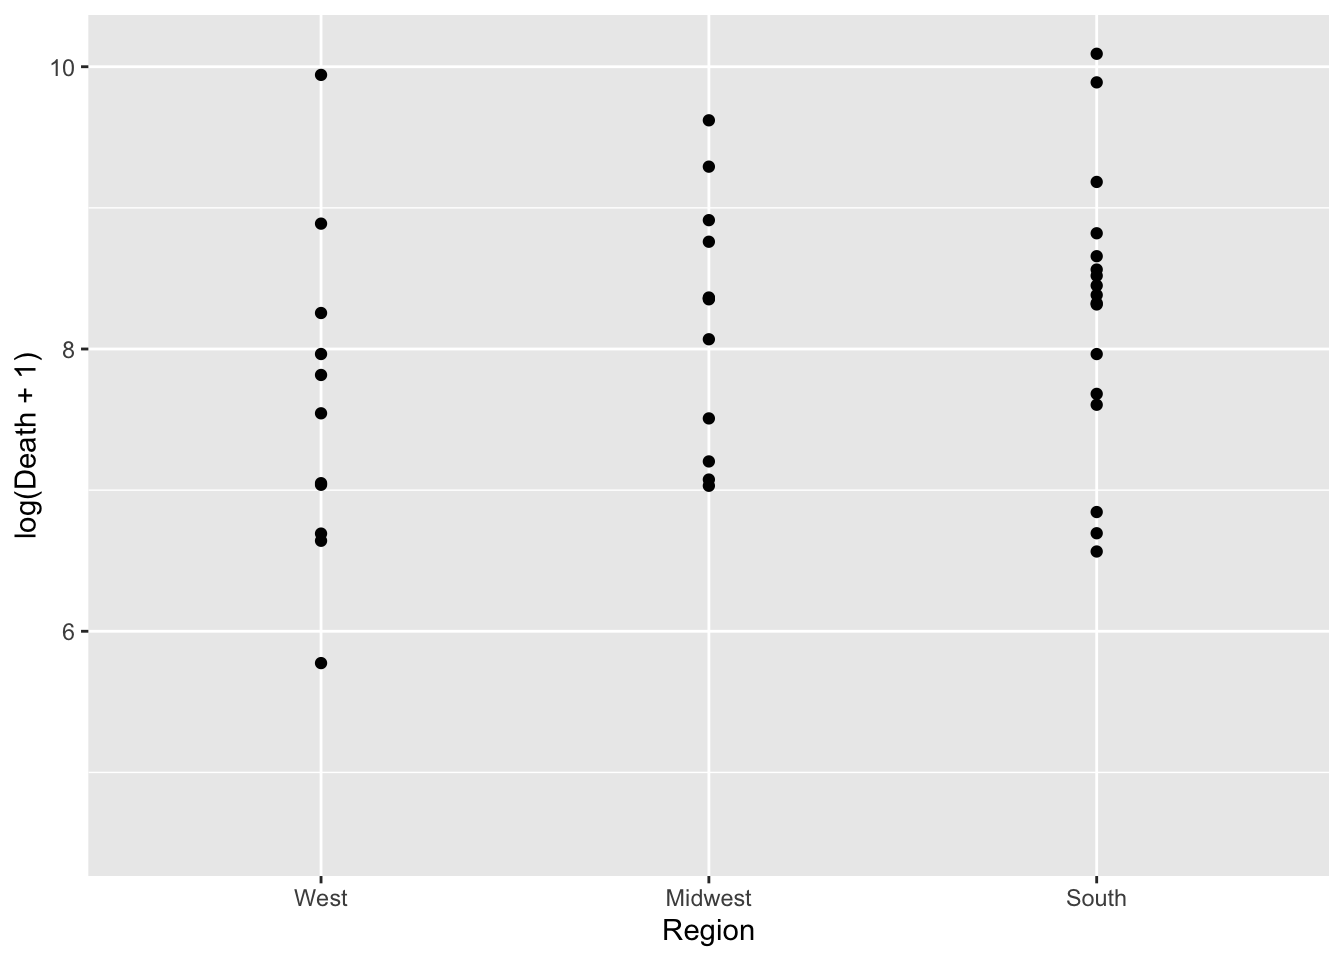
\includegraphics[width=0.5\linewidth]{bookdown-demo_files/figure-latex/xlimggplot2-1} 

}

\caption{Scatterplot with customized axis range for discrete features}\label{fig:xlimggplot2}
\end{figure}

\section{\texorpdfstring{Color Scales and Size of
\texttt{geom\_points()}}{Color Scales and Size of geom\_points()}}\label{color-scales-and-size-of-geom_points}

There are two ways of coloring. One approach is to color all points with
the same color. The other method is to color the points according to a
particular feature of the observation.

\subsection{Change the color of all
points}\label{change-the-color-of-all-points}

\begin{Shaded}
\begin{Highlighting}[]
\NormalTok{p }\OperatorTok{+}\StringTok{ }\KeywordTok{geom_point}\NormalTok{(}\DataTypeTok{color =} \StringTok{"blue"}\NormalTok{)}
\end{Highlighting}
\end{Shaded}

\begin{figure}

{\centering 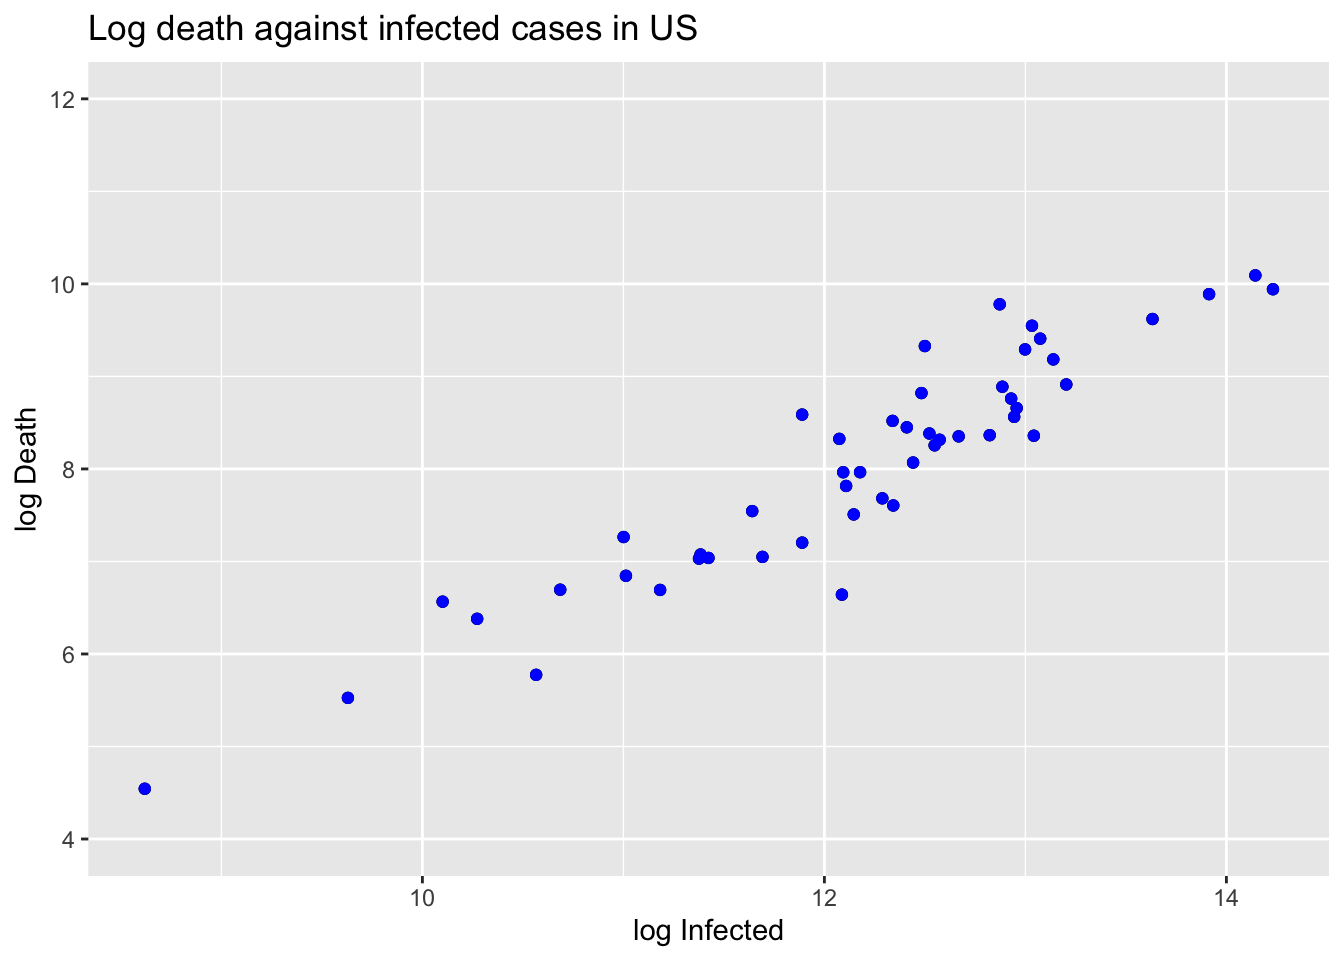
\includegraphics[width=0.5\linewidth]{bookdown-demo_files/figure-latex/unnamed-chunk-44-1} 

}

\caption{Scatterplot with all points colored blue}\label{fig:unnamed-chunk-44}
\end{figure}

\subsection{Color the observations by the value of a
feature}\label{color-the-observations-by-the-value-of-a-feature}

\begin{Shaded}
\begin{Highlighting}[]
\CommentTok{# Use Region as the feature for coloring}
\NormalTok{p }\OperatorTok{+}\StringTok{ }\KeywordTok{geom_point}\NormalTok{(}\KeywordTok{aes}\NormalTok{(}\DataTypeTok{color =}\NormalTok{ Region)) }
\CommentTok{# p + aes(color = Region) }

\CommentTok{# Use population for coloring}
\NormalTok{p }\OperatorTok{+}\StringTok{ }\KeywordTok{geom_point}\NormalTok{(}\KeywordTok{aes}\NormalTok{(}\DataTypeTok{color =}\NormalTok{ pop))}
\end{Highlighting}
\end{Shaded}

\begin{figure}
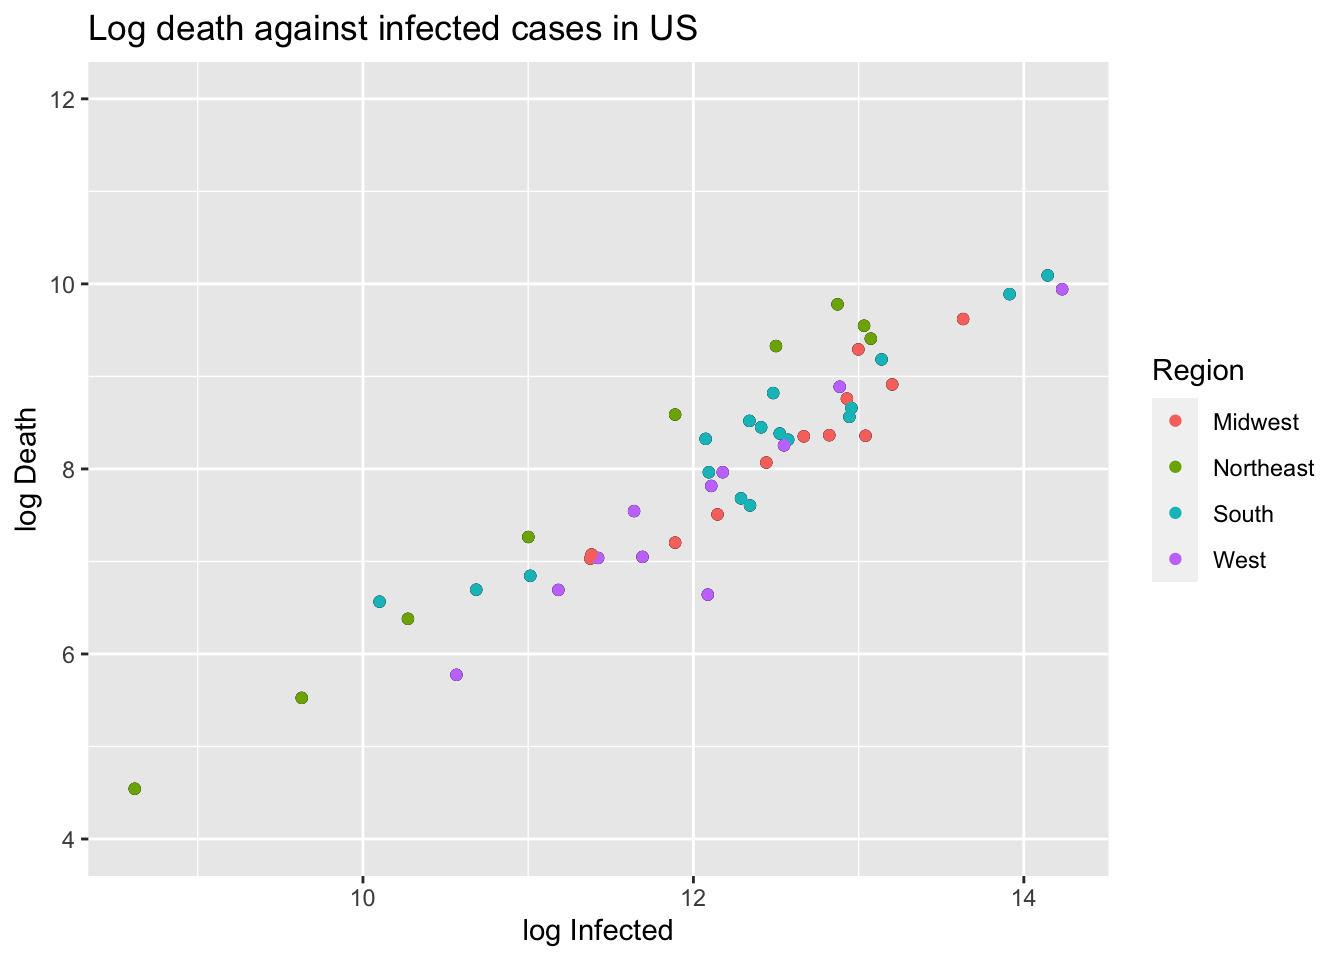
\includegraphics[width=0.5\linewidth]{bookdown-demo_files/figure-latex/unnamed-chunk-45-1} 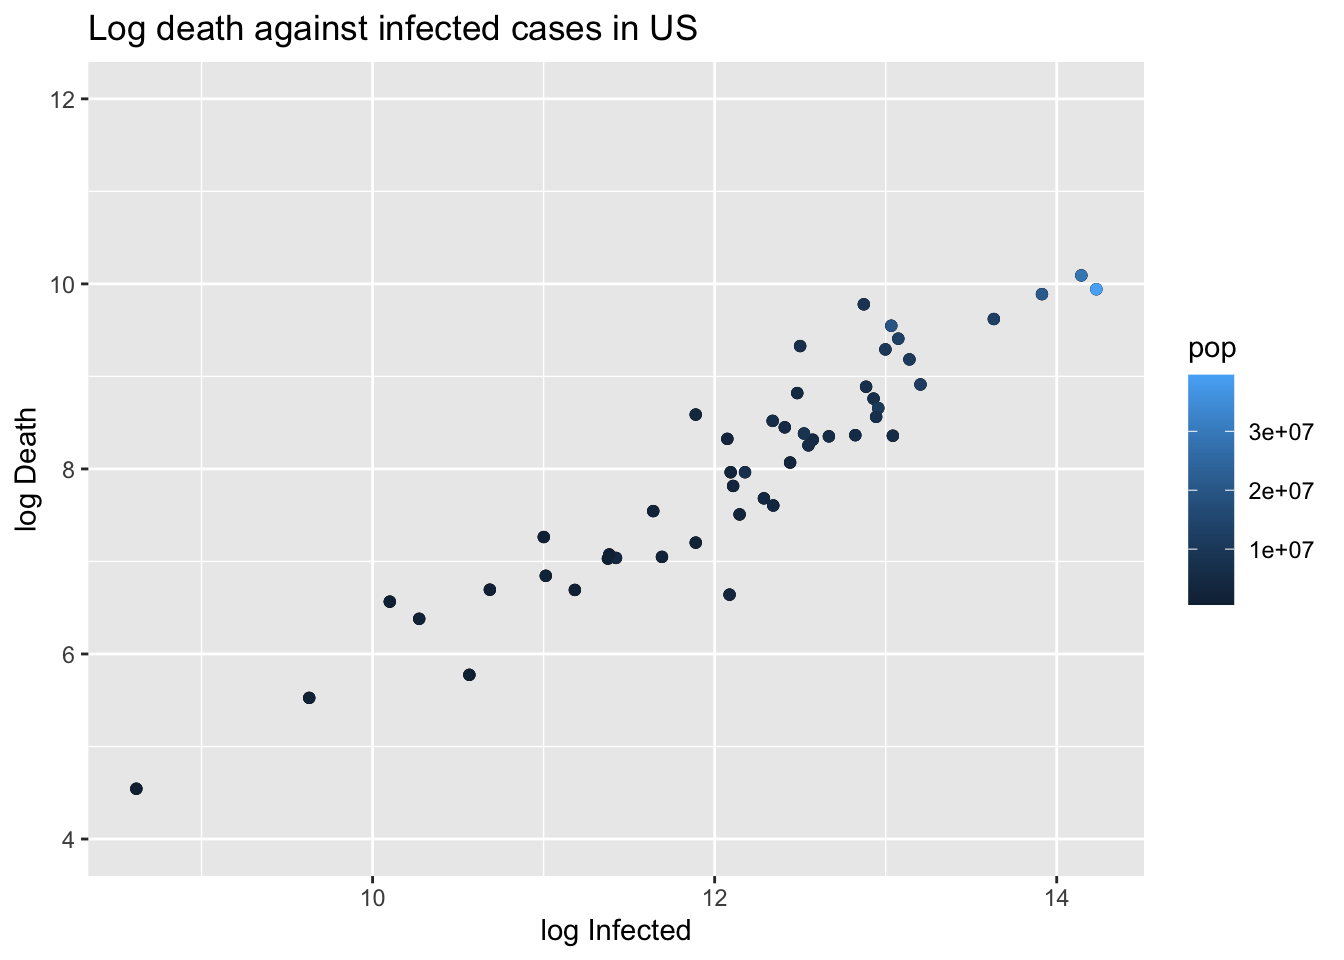
\includegraphics[width=0.5\linewidth]{bookdown-demo_files/figure-latex/unnamed-chunk-45-2} \caption{Scatterplot with points colored by Region or Population}\label{fig:unnamed-chunk-45}
\end{figure}

\textbf{Remarks:} the \texttt{color} feature is located at different
layers in three figures. In the first figure, it is under
\texttt{geom\_point()}, while in the latter two figures it is under
\texttt{geom\_point(aes())}. Because we only have one layer in this
example, we can equivalently use \texttt{aes()}, i.e., the aesthetic
mapping for the whole scatterplot.

\subsection{Change the color palette}\label{change-the-color-palette}

In addition, we can personalize the color palette using
\texttt{scale\_fill\_brewer()} for a discrete color scale, and
\texttt{scale\_fill\_distiller()} for a continuous color scale.

\begin{Shaded}
\begin{Highlighting}[]
\CommentTok{# Change the palette}
\CommentTok{# For discrete scale}
\NormalTok{p }\OperatorTok{+}\StringTok{ }\KeywordTok{geom_point}\NormalTok{(}\KeywordTok{aes}\NormalTok{(}\DataTypeTok{color =}\NormalTok{ Region)) }\OperatorTok{+}\StringTok{ }
\StringTok{   }\KeywordTok{scale_fill_brewer}\NormalTok{(}\DataTypeTok{palette =} \StringTok{"Set1"}\NormalTok{, }\DataTypeTok{aesthetics =} \StringTok{"color"}\NormalTok{)}
\CommentTok{# For continuous scale}
\NormalTok{p }\OperatorTok{+}\StringTok{ }\KeywordTok{geom_point}\NormalTok{(}\KeywordTok{aes}\NormalTok{(}\DataTypeTok{color =}\NormalTok{ pop)) }\OperatorTok{+}
\StringTok{ }\KeywordTok{scale_fill_distiller}\NormalTok{(}\DataTypeTok{palette =} \DecValTok{2}\NormalTok{, }\DataTypeTok{aesthetics =} \StringTok{"color"}\NormalTok{)}
\end{Highlighting}
\end{Shaded}

\begin{figure}
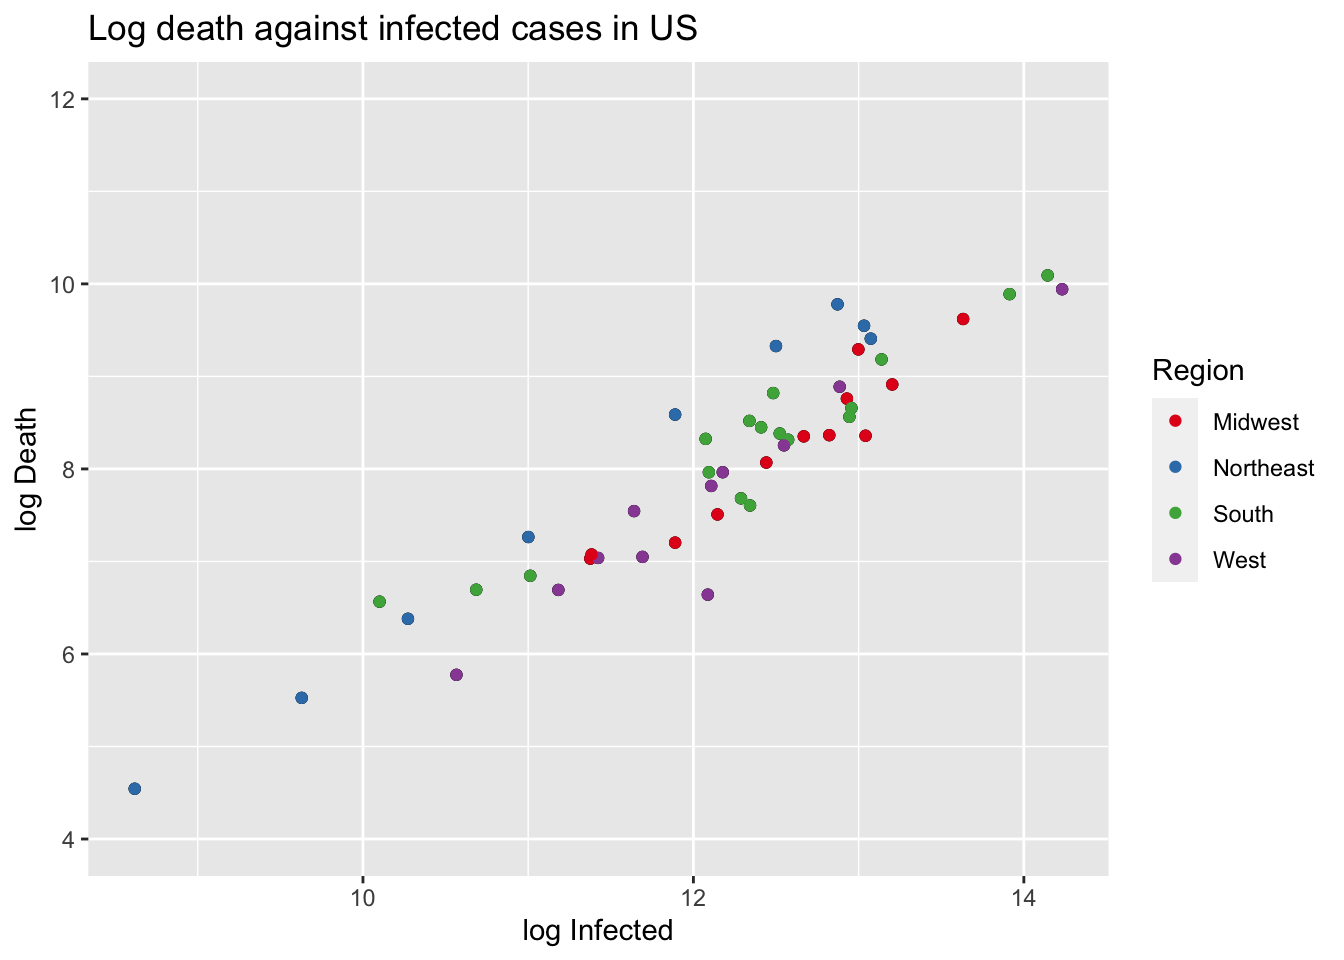
\includegraphics[width=0.5\linewidth]{bookdown-demo_files/figure-latex/unnamed-chunk-46-1} 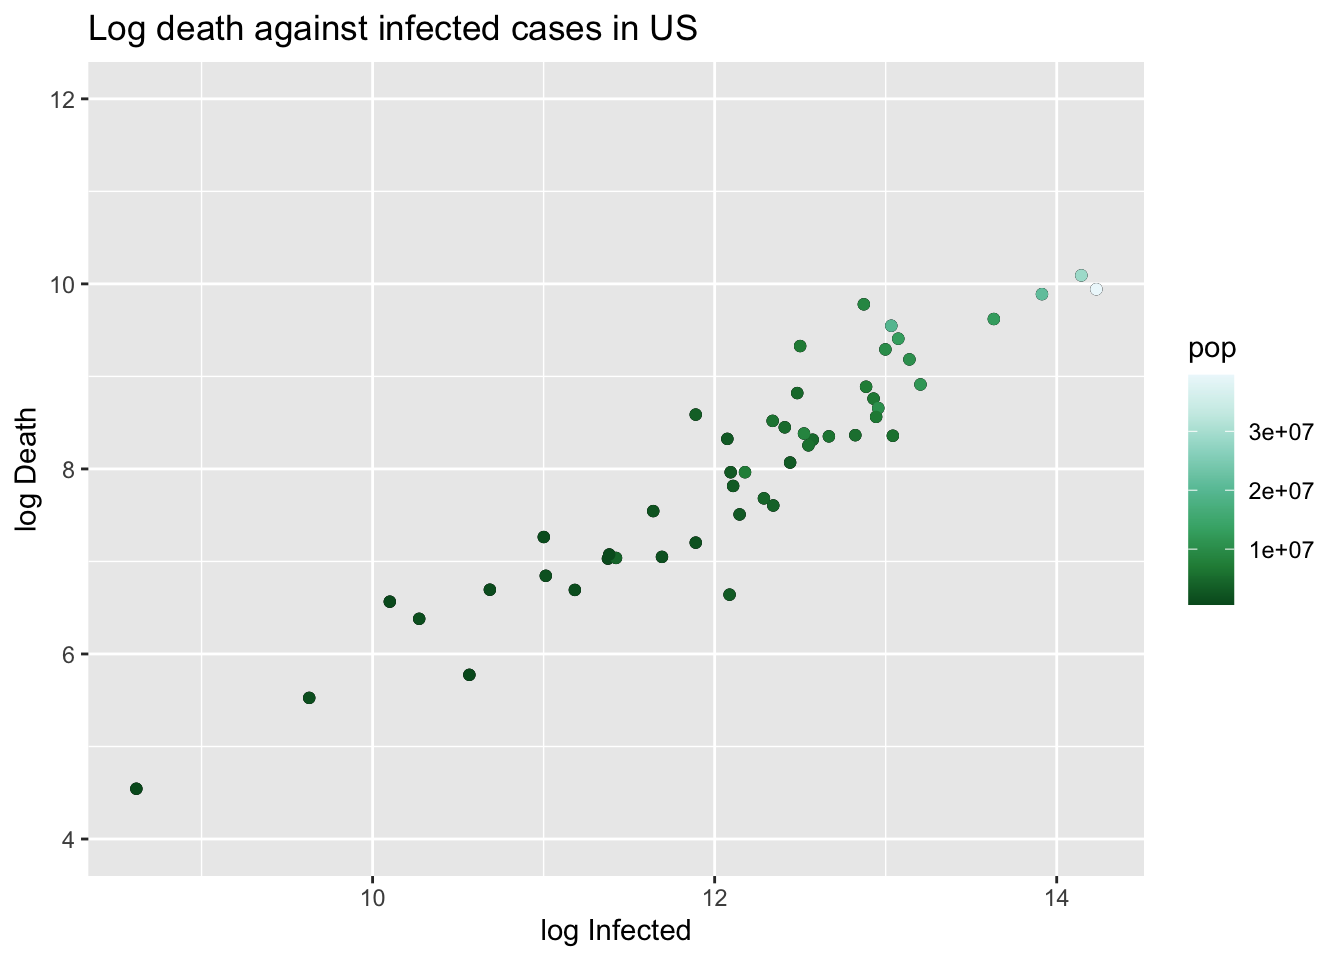
\includegraphics[width=0.5\linewidth]{bookdown-demo_files/figure-latex/unnamed-chunk-46-2} \caption{Scatterplot with customized color palette}\label{fig:unnamed-chunk-46}
\end{figure}

\subsection{Change the size by the value of a
feature}\label{change-the-size-by-the-value-of-a-feature}

\begin{Shaded}
\begin{Highlighting}[]
\NormalTok{p <-}\StringTok{ }\KeywordTok{ggplot}\NormalTok{(df, }\KeywordTok{aes}\NormalTok{(}\KeywordTok{log}\NormalTok{(Infected }\OperatorTok{+}\StringTok{ }\DecValTok{1}\NormalTok{), }\KeywordTok{log}\NormalTok{(Death }\OperatorTok{+}\StringTok{ }\DecValTok{1}\NormalTok{))) }\OperatorTok{+}
\StringTok{  }\KeywordTok{xlab}\NormalTok{(}\StringTok{'log Infected'}\NormalTok{) }\OperatorTok{+}
\StringTok{  }\KeywordTok{ylab}\NormalTok{(}\StringTok{'log Death'}\NormalTok{) }\OperatorTok{+}\StringTok{ }
\StringTok{  }\KeywordTok{labs}\NormalTok{(}\DataTypeTok{title =} \StringTok{'Log death against infected cases in US'}\NormalTok{)}

\CommentTok{# Change the point size}
\NormalTok{p }\OperatorTok{+}\StringTok{ }\KeywordTok{geom_point}\NormalTok{(}\KeywordTok{aes}\NormalTok{ (}\DataTypeTok{size =}\NormalTok{ pop))}

\CommentTok{# Change the point color and size}
\NormalTok{p }\OperatorTok{+}\StringTok{ }\KeywordTok{geom_point}\NormalTok{(}\KeywordTok{aes}\NormalTok{ (}\DataTypeTok{size =}\NormalTok{ pop , }\DataTypeTok{color =}\NormalTok{ pop))}
\end{Highlighting}
\end{Shaded}

\begin{figure}
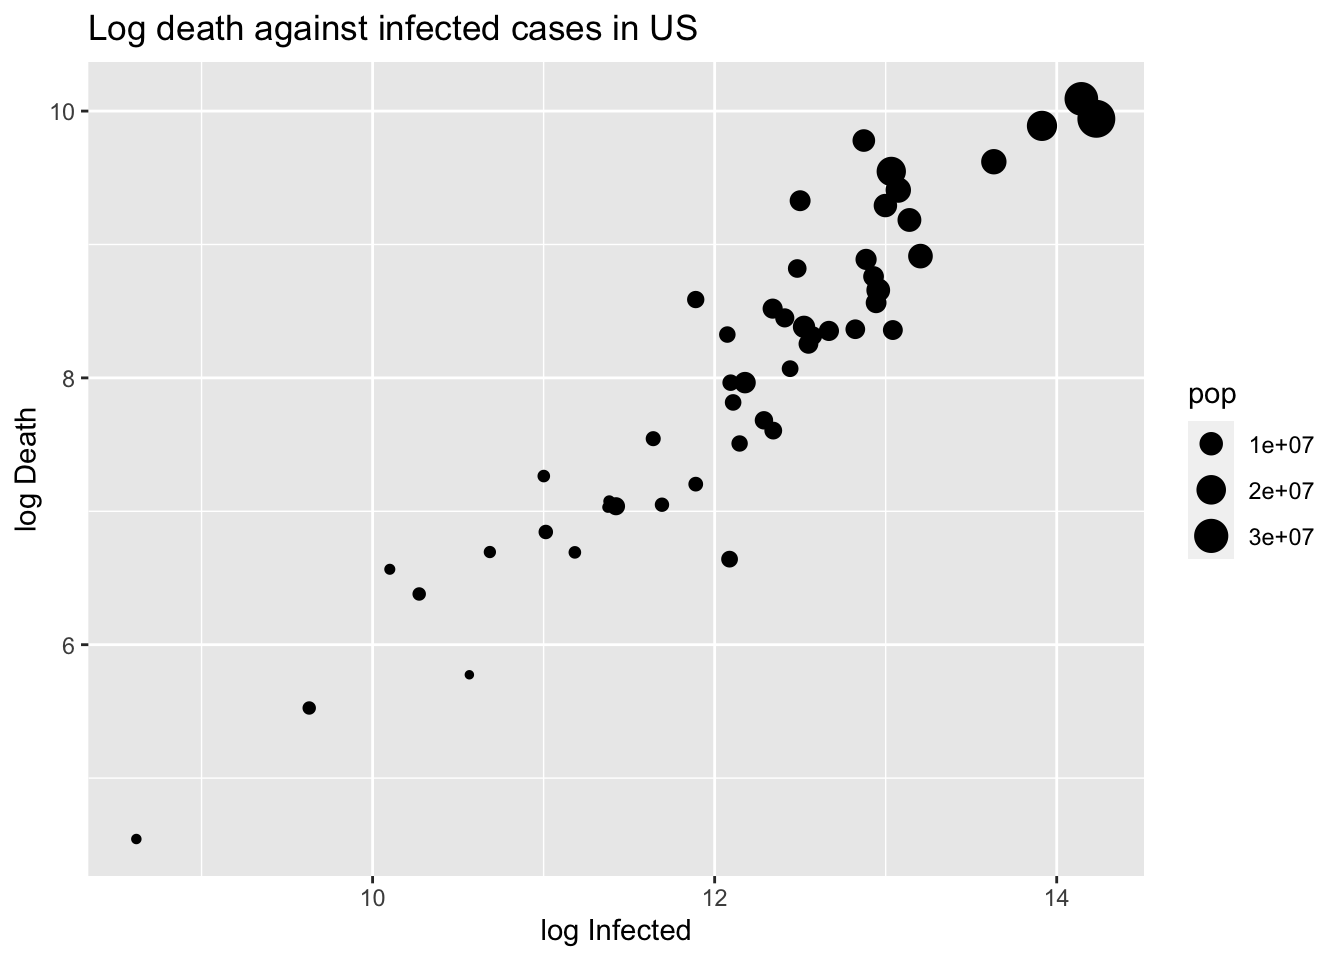
\includegraphics[width=0.5\linewidth]{bookdown-demo_files/figure-latex/unnamed-chunk-47-1} 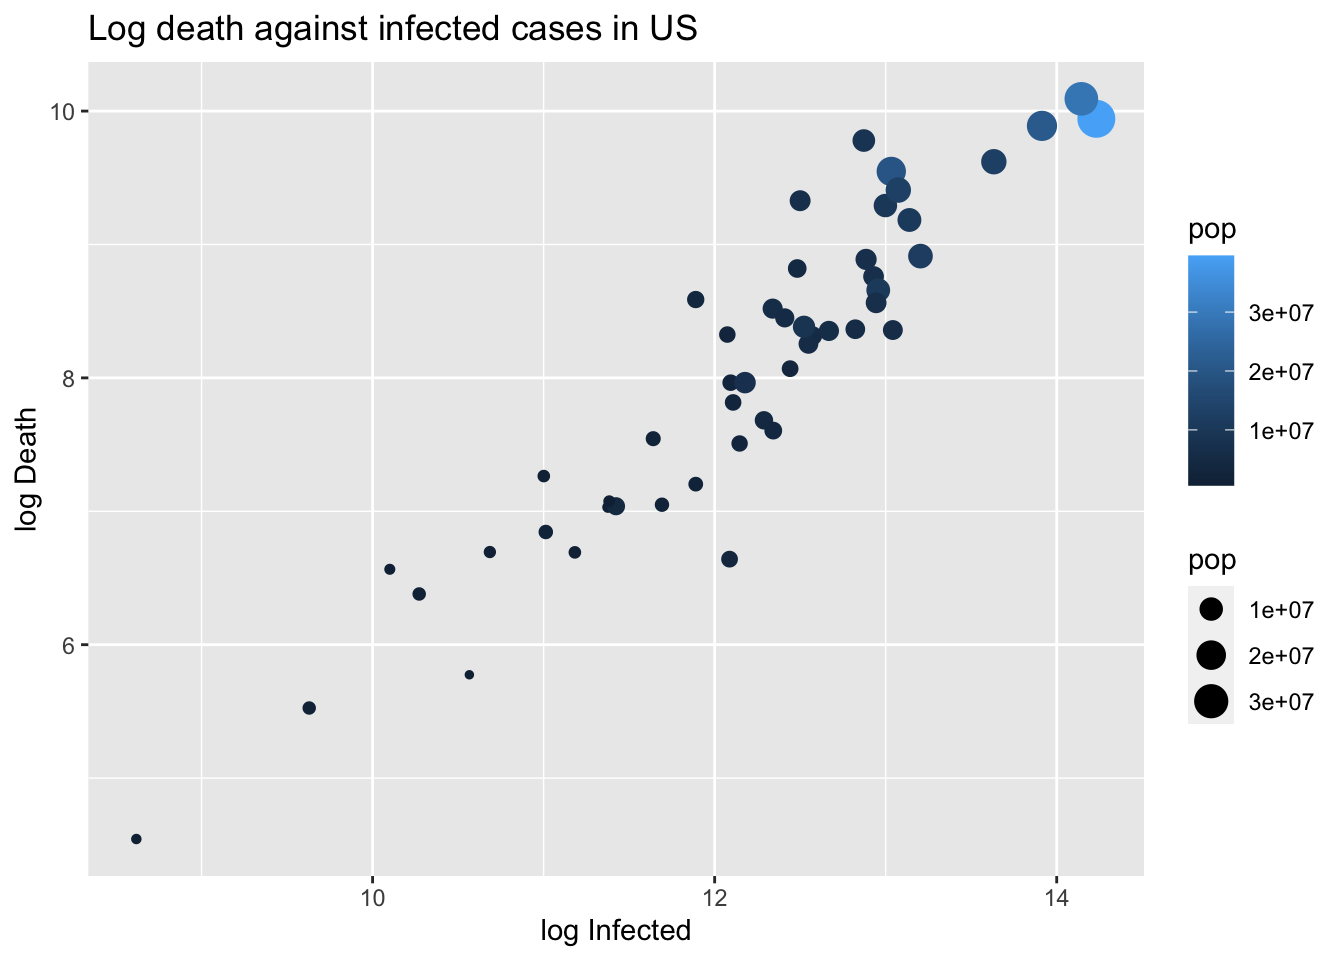
\includegraphics[width=0.5\linewidth]{bookdown-demo_files/figure-latex/unnamed-chunk-47-2} \caption{Scatterplot with customized point size or color}\label{fig:unnamed-chunk-47}
\end{figure}

\begin{Shaded}
\begin{Highlighting}[]
\CommentTok{# Combine the color and size in legend}
\CommentTok{# Method 1: keep the size and color the same limits and breaks}
\NormalTok{p }\OperatorTok{+}\StringTok{ }\KeywordTok{geom_point}\NormalTok{(}\KeywordTok{aes}\NormalTok{ (}\DataTypeTok{size =}\NormalTok{ pop, }\DataTypeTok{color =}\NormalTok{ pop)) }\OperatorTok{+}
\StringTok{  }\KeywordTok{scale_color_continuous}\NormalTok{(}\DataTypeTok{limits =} \KeywordTok{c}\NormalTok{(}\FloatTok{0e7}\NormalTok{, }\FloatTok{4e7}\NormalTok{), }
                         \DataTypeTok{breaks =} \KeywordTok{seq}\NormalTok{(}\DecValTok{0}\NormalTok{, }\FloatTok{4e7}\NormalTok{, }\DataTypeTok{by =} \FloatTok{1e7}\NormalTok{)) }\OperatorTok{+}
\StringTok{  }\KeywordTok{scale_size_area}\NormalTok{(}\DataTypeTok{limits =} \KeywordTok{c}\NormalTok{(}\FloatTok{0e7}\NormalTok{, }\FloatTok{4e7}\NormalTok{), }
                  \DataTypeTok{breaks =} \KeywordTok{seq}\NormalTok{(}\DecValTok{0}\NormalTok{, }\FloatTok{4e7}\NormalTok{, }\DataTypeTok{by =} \FloatTok{1e7}\NormalTok{), }\DataTypeTok{max_size =} \DecValTok{12}\NormalTok{) }\OperatorTok{+}
\StringTok{  }\KeywordTok{guides}\NormalTok{(}\DataTypeTok{color =} \KeywordTok{guide_legend}\NormalTok{(), }\DataTypeTok{size =} \KeywordTok{guide_legend}\NormalTok{()) }

\CommentTok{# Method 2: use scale_color_gradient and scale_size}
\NormalTok{p <-}\StringTok{ }\NormalTok{p }\OperatorTok{+}\StringTok{ }\KeywordTok{geom_point}\NormalTok{(}\KeywordTok{aes}\NormalTok{(}\DataTypeTok{size =}\NormalTok{ pop, }\DataTypeTok{color =}\NormalTok{ pop), }\DataTypeTok{alpha =} \FloatTok{0.7}\NormalTok{) }\OperatorTok{+}
\StringTok{   }\KeywordTok{scale_color_gradient}\NormalTok{(}\DataTypeTok{low =} \StringTok{"lightblue"}\NormalTok{, }\DataTypeTok{high =} \StringTok{"red"}\NormalTok{) }\OperatorTok{+}
\StringTok{   }\KeywordTok{scale_size_area}\NormalTok{(}\DataTypeTok{max_size =} \DecValTok{12}\NormalTok{) }\OperatorTok{+}
\StringTok{   }\KeywordTok{guides}\NormalTok{(}\DataTypeTok{color =} \KeywordTok{guide_legend}\NormalTok{(), }\DataTypeTok{size =} \KeywordTok{guide_legend}\NormalTok{())}

\NormalTok{p}
\end{Highlighting}
\end{Shaded}

\begin{figure}
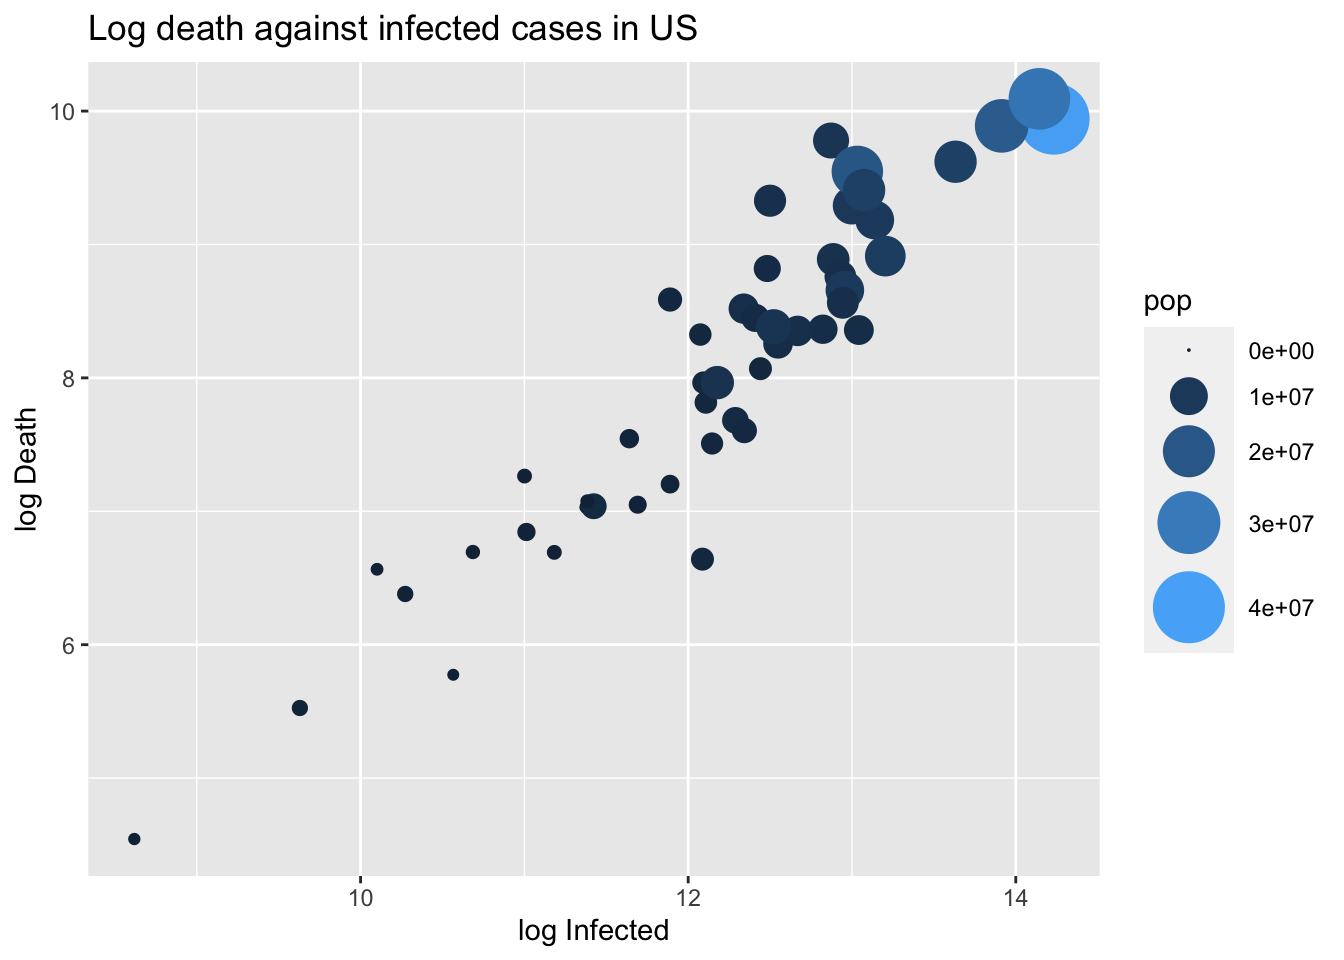
\includegraphics[width=0.5\linewidth]{bookdown-demo_files/figure-latex/unnamed-chunk-48-1} 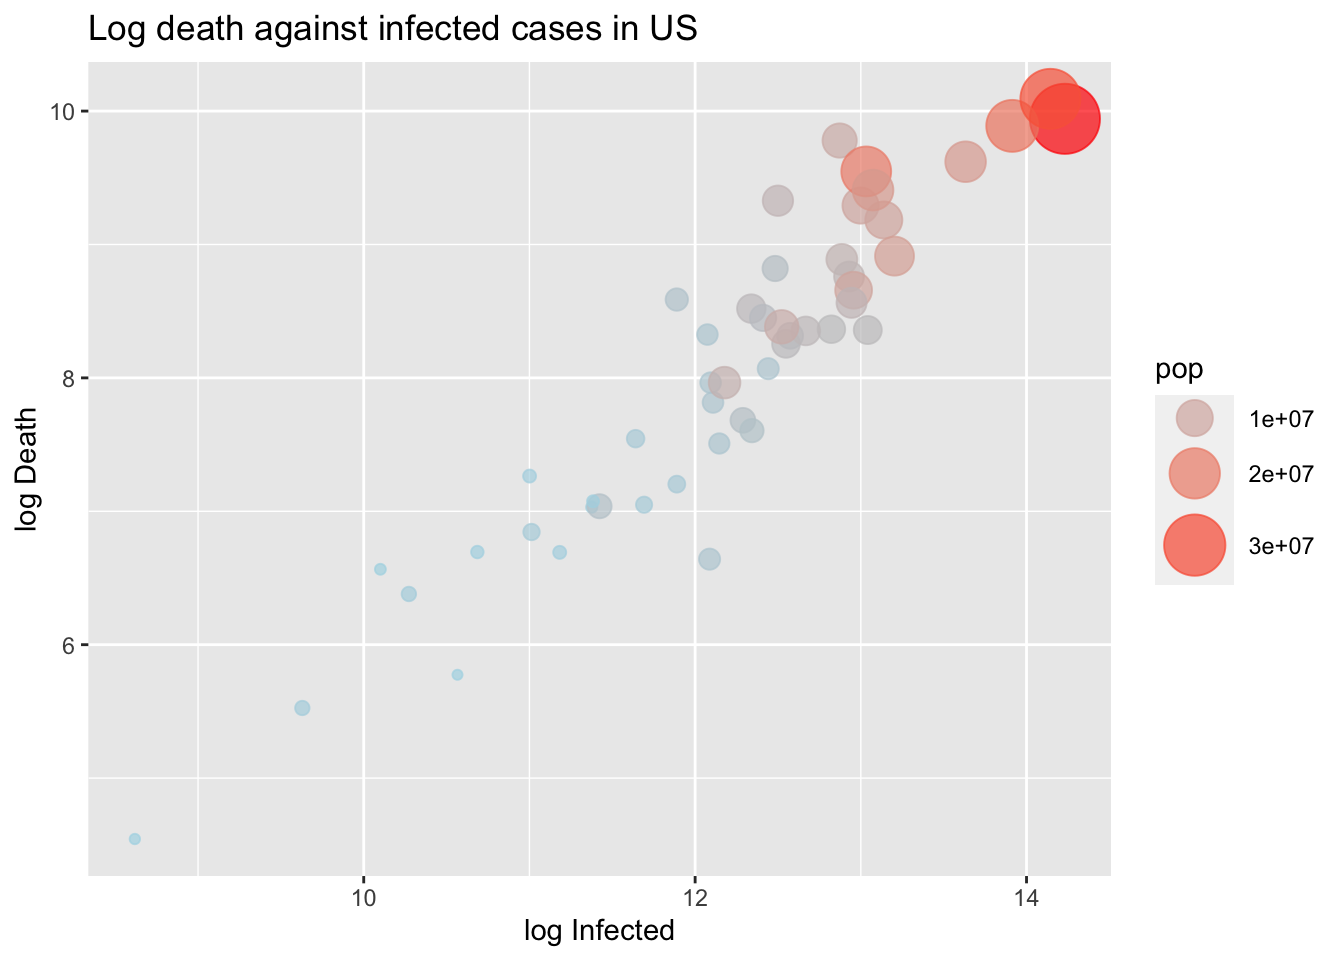
\includegraphics[width=0.5\linewidth]{bookdown-demo_files/figure-latex/unnamed-chunk-48-2} \caption{Scatterplot with customized point color and point size}\label{fig:unnamed-chunk-48}
\end{figure}

\textbf{Remarks:} For Method 1, the key to combining two aesthetic
settings of the layer to one legend, in this case, \texttt{color} and
\texttt{size}, is to set the \texttt{limits} and \texttt{breaks} to be
the same in \texttt{guides}. For both methods,
\texttt{guides(color\ =\ guide\_legend(),\ size\ =\ guide\_legend())} is
needed.

\section{Individual geoms}\label{individual-geoms}

Apart from the scatter plot, there are many individual geoms, for
example:

\begin{itemize}
\tightlist
\item
  \texttt{geom\_line()}: line graphs
\item
  \texttt{geom\_boxplot()}:boxplots
\item
  \texttt{geom\_bar()}: bar chart
\item
  \texttt{geom\_histogram()}: histogram plots
\item
  \texttt{geom\_smooth()}: regression lines or curves
\end{itemize}

We introduce a few of them in detail as follows.

\subsection{Histogram}\label{histogram}

The histogram is an important tool to summarize the range and frequency
of observations. Here we plot the histogram of log daily new infected
cases counts using using \texttt{geom\_histogram}. We can adjust the
option \texttt{binwidth} to control the widths of the bins.

\begin{Shaded}
\begin{Highlighting}[]
\CommentTok{# Prepare the daily new Infected for each state }
\CommentTok{# in the period 2020-11-12 to 2020-12-11}
\NormalTok{df <-}\StringTok{ }\NormalTok{slid}\OperatorTok{::}\NormalTok{state.long }\OperatorTok\StringTok{ }
\StringTok{  }\NormalTok{dplyr}\OperatorTok{::}\KeywordTok{filter}\NormalTok{(DATE }\OperatorTok{<=}\StringTok{ '2020-12-11'} \OperatorTok{&}\StringTok{ }\NormalTok{DATE }\OperatorTok{>}\StringTok{ '2020-11-11'}\NormalTok{) }\OperatorTok
\StringTok{  }\KeywordTok{group_by}\NormalTok{(State) }\OperatorTok\StringTok{ }\CommentTok{# Group by State}
\StringTok{  }\KeywordTok{mutate}\NormalTok{(}\DataTypeTok{Y.Infected =} 
           \KeywordTok{c}\NormalTok{(Infected[}\OperatorTok{-}\KeywordTok{length}\NormalTok{(Infected)] }\OperatorTok{-}\StringTok{ }\NormalTok{Infected[}\OperatorTok{-}\DecValTok{1}\NormalTok{], }\DecValTok{0}\NormalTok{)) }
\NormalTok{df}
\end{Highlighting}
\end{Shaded}

\begin{verbatim}
## # A tibble: 1,470 x 8
## # Groups:   State [49]
##    State Region Division    pop DATE       Infected Death
##    <fct> <fct>  <fct>     <int> <date>        <int> <int>
##  1 Alab~ South  East So~ 4.89e6 2020-12-11   288775  4086
##  2 Alab~ South  East So~ 4.89e6 2020-12-10   284922  4034
##  3 Alab~ South  East So~ 4.89e6 2020-12-09   280187  3985
##  4 Alab~ South  East So~ 4.89e6 2020-12-08   276665  3940
##  5 Alab~ South  East So~ 4.89e6 2020-12-07   272228  3891
##  6 Alab~ South  East So~ 4.89e6 2020-12-06   269877  3888
##  7 Alab~ South  East So~ 4.89e6 2020-12-05   267589  3876
##  8 Alab~ South  East So~ 4.89e6 2020-12-04   264199  3831
##  9 Alab~ South  East So~ 4.89e6 2020-12-03   260359  3776
## 10 Alab~ South  East So~ 4.89e6 2020-12-02   256828  3711
## # ... with 1,460 more rows, and 1 more variable:
## #   Y.Infected <dbl>
\end{verbatim}

\begin{Shaded}
\begin{Highlighting}[]
\NormalTok{p <-}\StringTok{ }\KeywordTok{ggplot}\NormalTok{(df, }\KeywordTok{aes}\NormalTok{(}\KeywordTok{log}\NormalTok{(Y.Infected }\OperatorTok{+}\StringTok{ }\DecValTok{1}\NormalTok{))) }
\NormalTok{p }\OperatorTok{+}\StringTok{ }\KeywordTok{geom_histogram}\NormalTok{(}\DataTypeTok{binwidth =} \DecValTok{1}\NormalTok{)}
\NormalTok{p }\OperatorTok{+}\StringTok{ }\KeywordTok{geom_histogram}\NormalTok{(}\DataTypeTok{binwidth =} \DecValTok{1}\NormalTok{) }\OperatorTok{+}\StringTok{ }\KeywordTok{aes}\NormalTok{(}\DataTypeTok{fill =}\NormalTok{ Region) }
\end{Highlighting}
\end{Shaded}

\begin{figure}
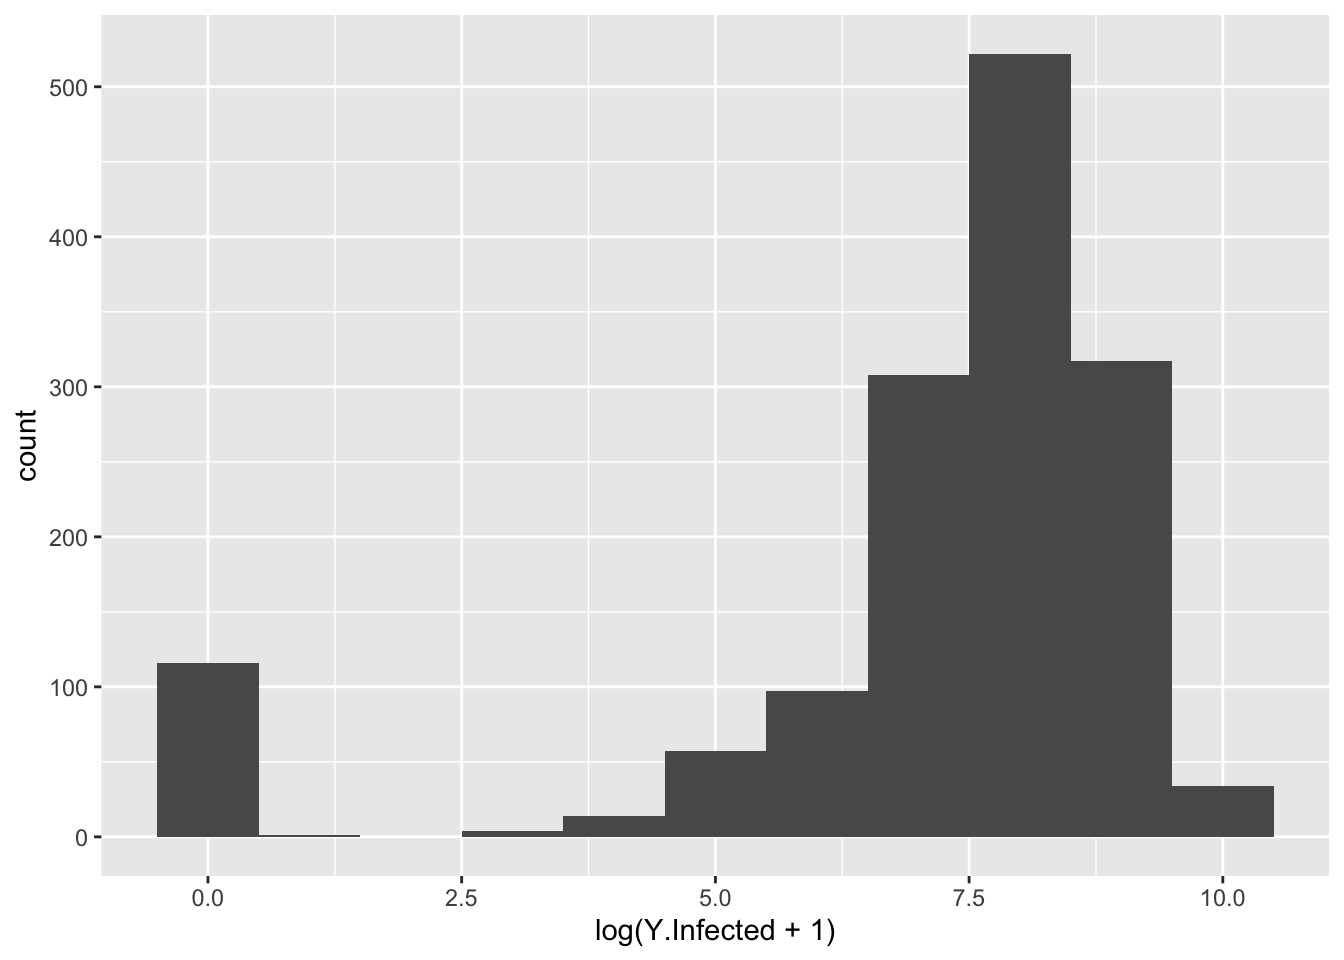
\includegraphics[width=0.5\linewidth]{bookdown-demo_files/figure-latex/Histogram-1} 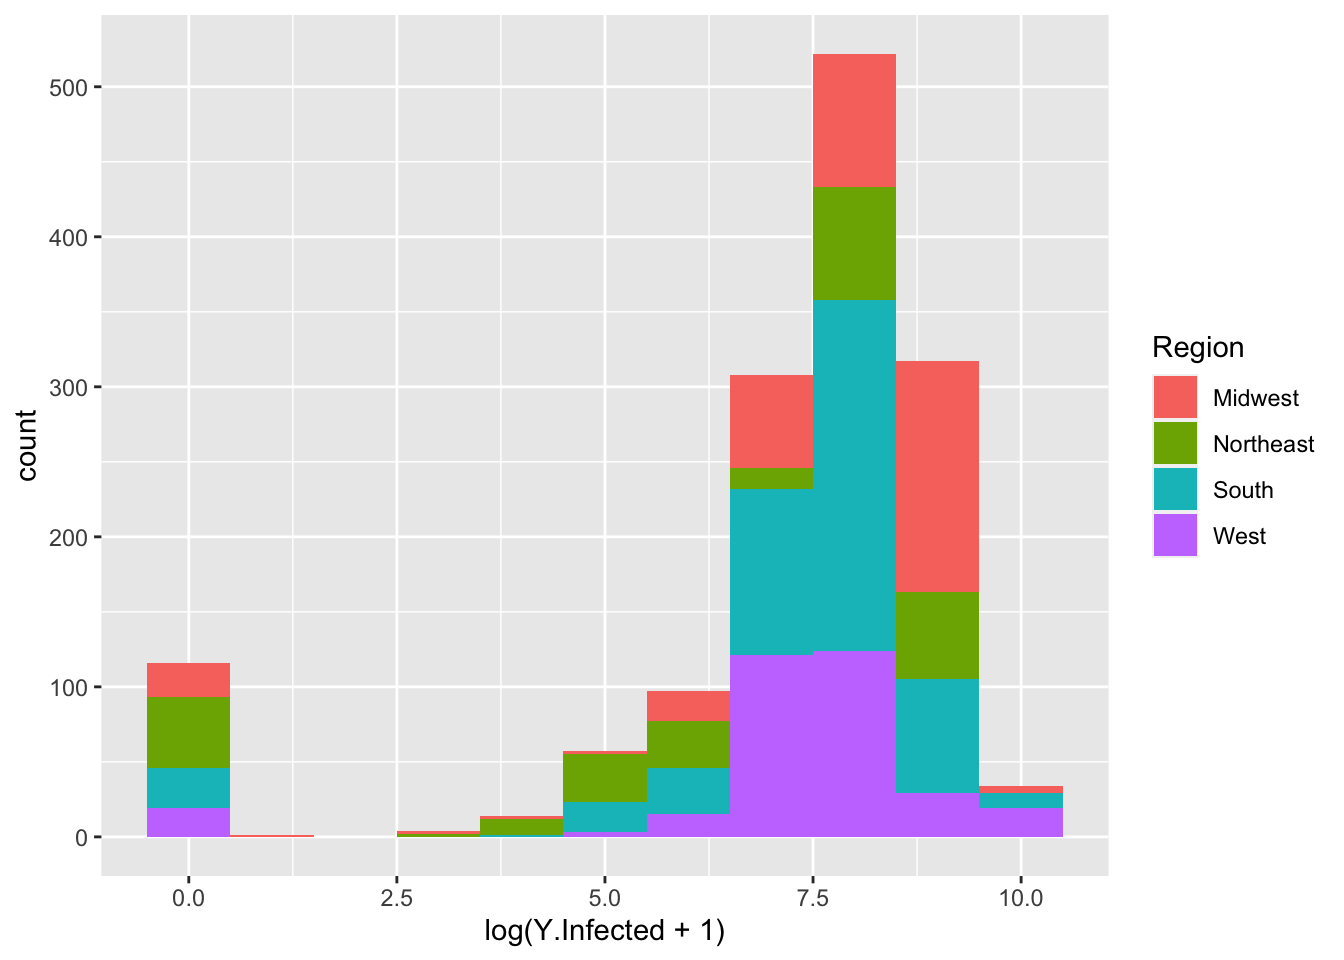
\includegraphics[width=0.5\linewidth]{bookdown-demo_files/figure-latex/Histogram-2} \caption{Histogram examples}\label{fig:Histogram}
\end{figure}

\subsection{Bar chart}\label{bar-chart}

The discrete analogue of histogram is the bar chart.

\subsection{Default bar chart}\label{default-bar-chart}

The default \texttt{geom\_bar()}, or equivalently
\texttt{geom\_bar(stat=\textquotesingle{}count\textquotesingle{})},
counts the number of observations in each category shown as following.
This plot essentially tells us how many states there are in each region.

\begin{Shaded}
\begin{Highlighting}[]
\NormalTok{df <-}\StringTok{ }\NormalTok{slid}\OperatorTok{::}\NormalTok{state.long }\OperatorTok\StringTok{ }
\StringTok{  }\NormalTok{dplyr}\OperatorTok{::}\KeywordTok{filter}\NormalTok{(DATE }\OperatorTok{==}\StringTok{ }\KeywordTok{as.Date}\NormalTok{(}\StringTok{'2020-12-11'}\NormalTok{)) }
\NormalTok{p <-}\StringTok{ }\KeywordTok{ggplot}\NormalTok{(df, }\KeywordTok{aes}\NormalTok{(Region))}
\NormalTok{p }\OperatorTok{+}\StringTok{ }\KeywordTok{geom_bar}\NormalTok{()}
\end{Highlighting}
\end{Shaded}

\begin{figure}

{\centering 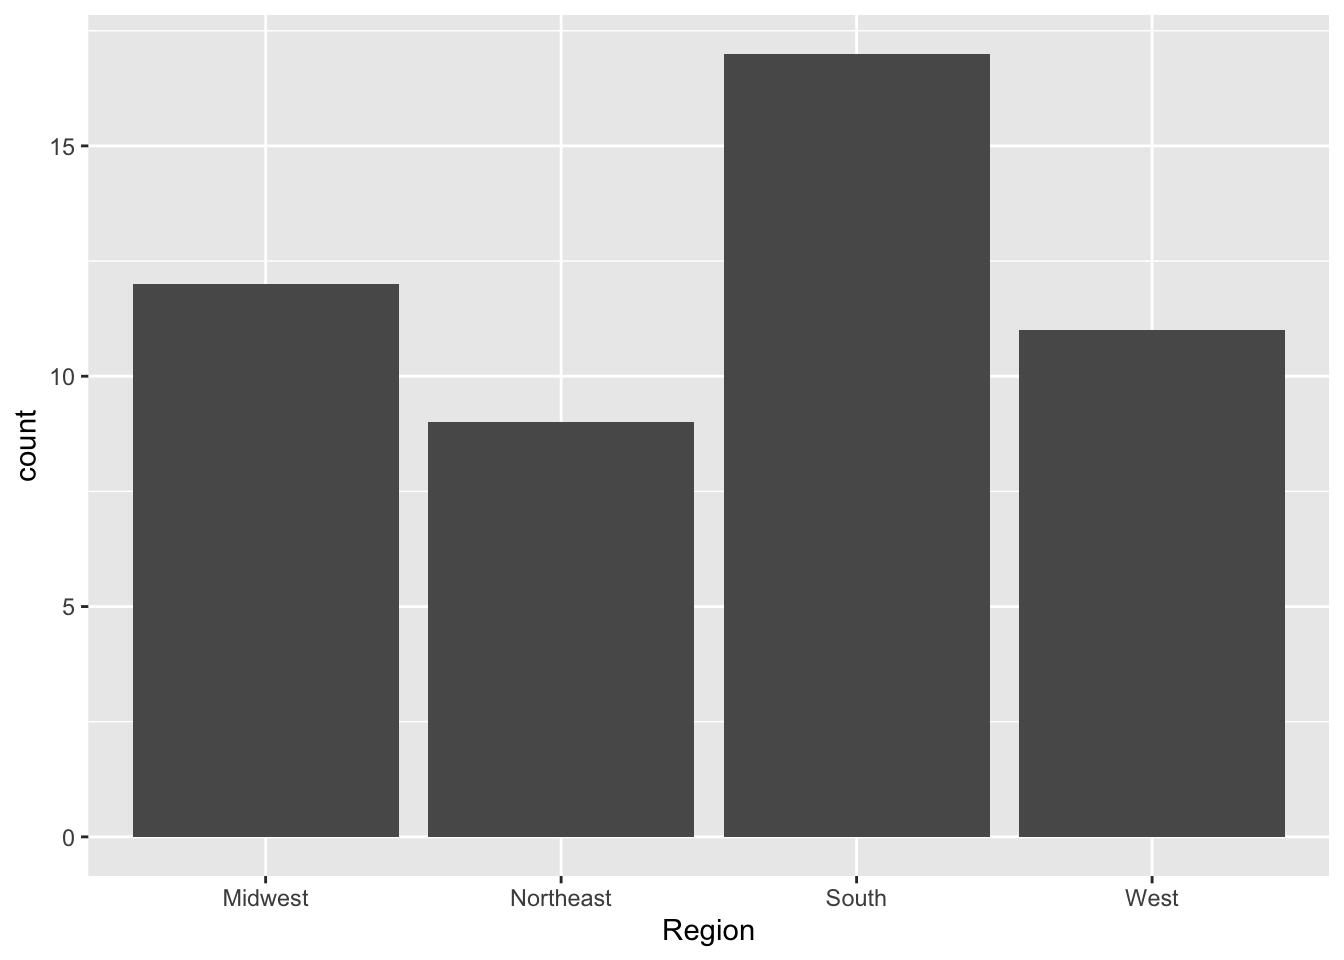
\includegraphics[width=0.5\linewidth]{bookdown-demo_files/figure-latex/Boxplot1-1} 

}

\caption{Bar plot example}\label{fig:Boxplot1}
\end{figure}

\subsection{Bar chart with assigned
value}\label{bar-chart-with-assigned-value}

In addition to the previous example, we can assign the height of the
bars by ourselves by using the option
\texttt{geom\_bar(stat\ =\ \textquotesingle{}identity\textquotesingle{})}.
In that case, we tell \texttt{geom\_bar} to use \texttt{y} value in the
data frame as the height of the bars.

\begin{Shaded}
\begin{Highlighting}[]
\NormalTok{df <-}\StringTok{ }\NormalTok{slid}\OperatorTok{::}\NormalTok{state.long }\OperatorTok\StringTok{ }
\StringTok{  }\NormalTok{dplyr}\OperatorTok{::}\KeywordTok{filter}\NormalTok{(DATE }\OperatorTok{==}\StringTok{ }\KeywordTok{as.Date}\NormalTok{(}\StringTok{'2020-12-11'}\NormalTok{)) }
\NormalTok{p <-}\StringTok{ }\KeywordTok{ggplot}\NormalTok{(df, }\KeywordTok{aes}\NormalTok{(Region, Infected)) }
\NormalTok{p }\OperatorTok{+}\StringTok{ }\KeywordTok{geom_bar}\NormalTok{(}\DataTypeTok{stat =} \StringTok{'identity'}\NormalTok{) }
\NormalTok{p }\OperatorTok{+}\StringTok{ }\KeywordTok{geom_bar}\NormalTok{(}\DataTypeTok{stat =} \StringTok{'identity'}\NormalTok{, }\KeywordTok{aes}\NormalTok{(}\DataTypeTok{fill =}\NormalTok{ Division))}
\end{Highlighting}
\end{Shaded}

\begin{figure}
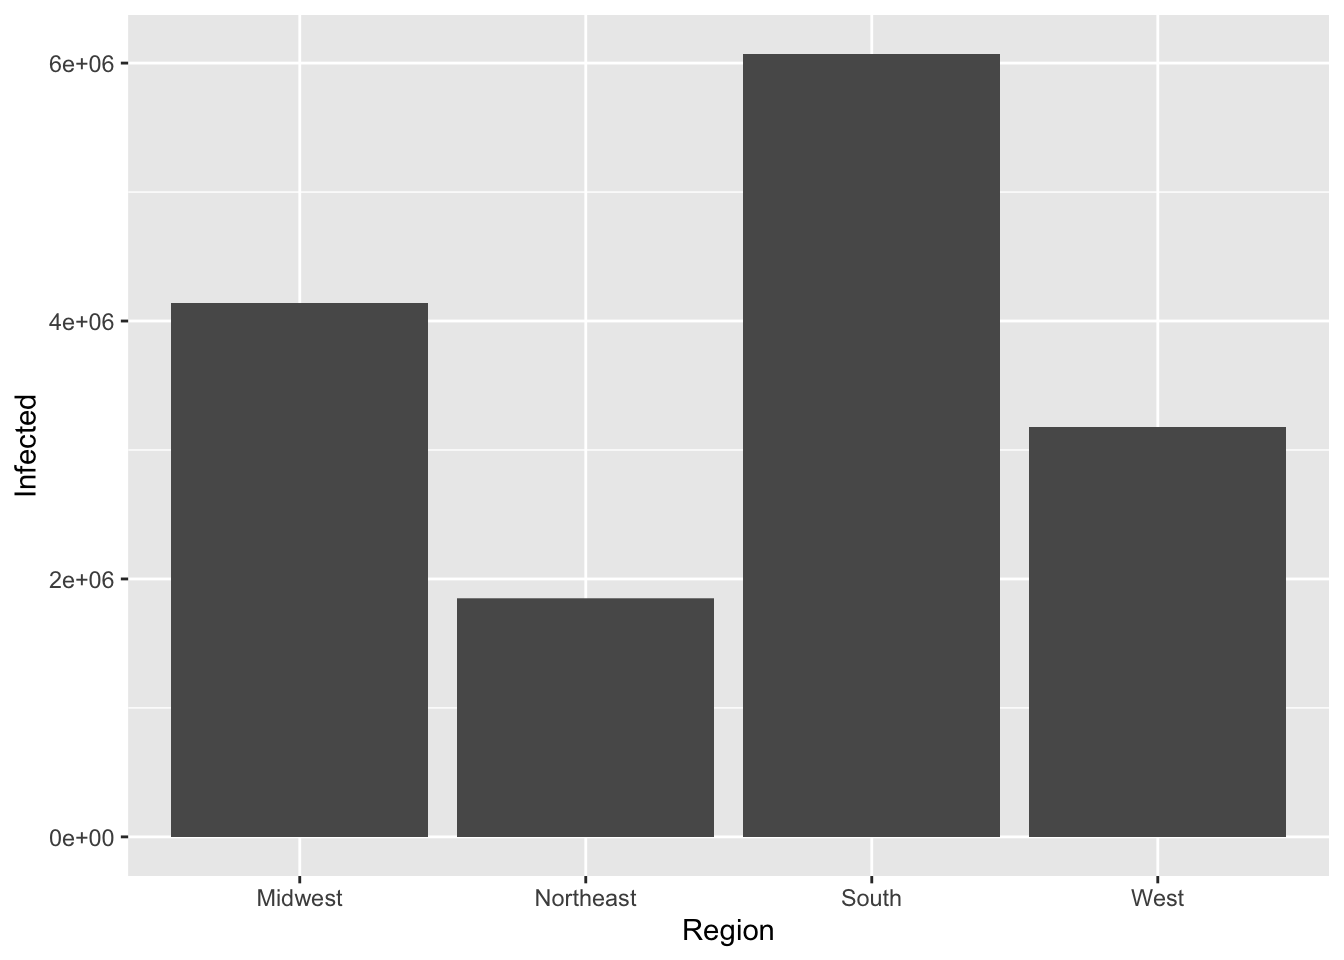
\includegraphics[width=0.5\linewidth]{bookdown-demo_files/figure-latex/Boxplot2-1} 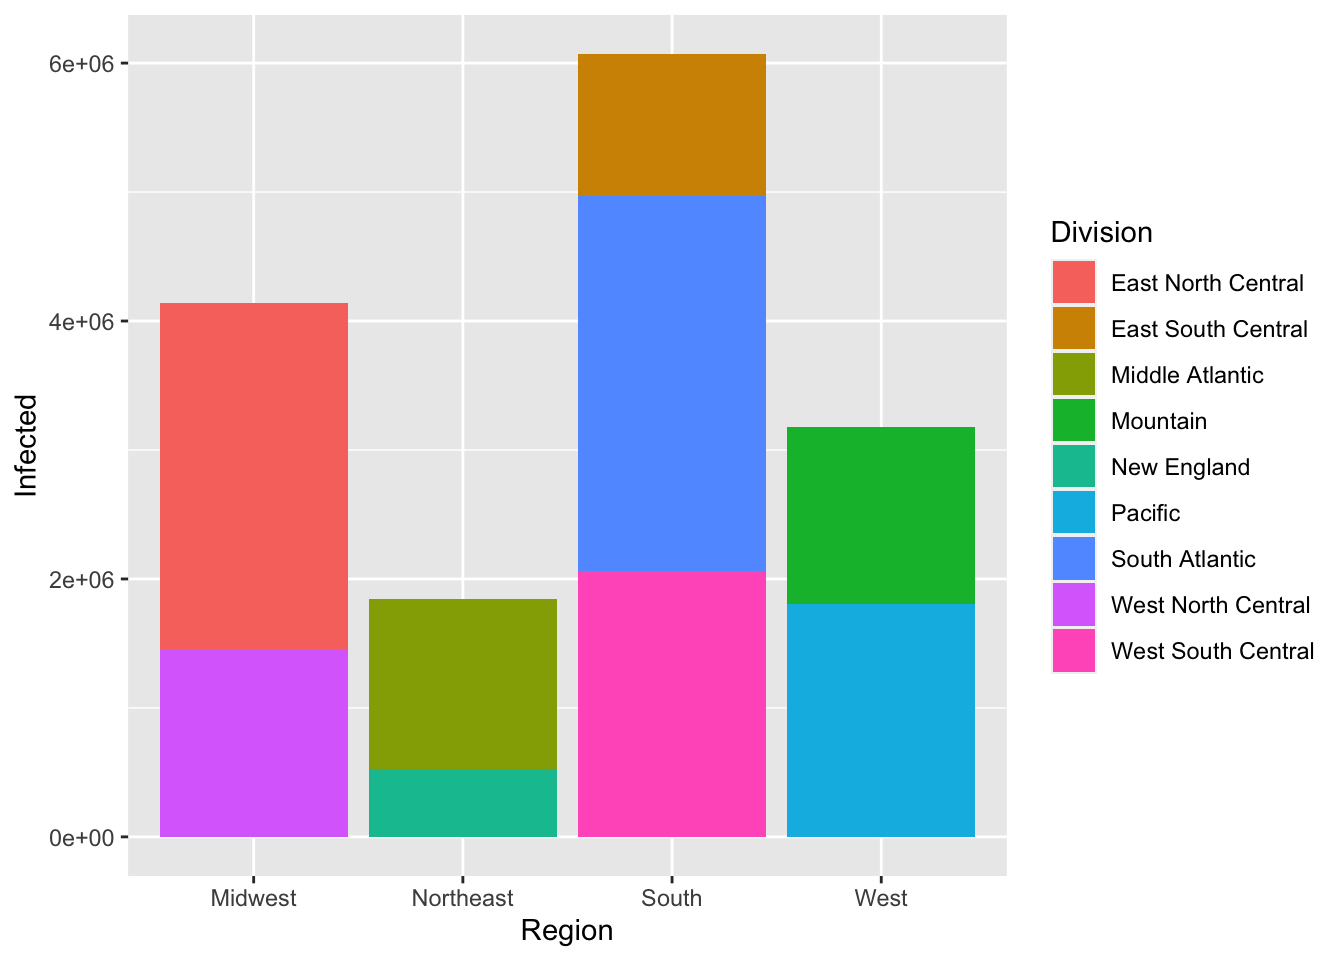
\includegraphics[width=0.5\linewidth]{bookdown-demo_files/figure-latex/Boxplot2-2} \caption{Bar plot with assigned values}\label{fig:Boxplot2}
\end{figure}

\subsection{Legend}\label{legend}

\begin{enumerate}
\def\labelenumi{\arabic{enumi}.}
\tightlist
\item
  Legend position
\end{enumerate}

We can adjust the position of the legends using
\texttt{theme(legend.position\ =\ \textquotesingle{}left/right/bottom/none\textquotesingle{})}.

\begin{Shaded}
\begin{Highlighting}[]
\NormalTok{p <-}\StringTok{ }\KeywordTok{ggplot}\NormalTok{(df, }\KeywordTok{aes}\NormalTok{(Region, }\DataTypeTok{fill =}\NormalTok{ Region)) }\OperatorTok{+}
\StringTok{  }\KeywordTok{ylab}\NormalTok{(}\StringTok{'Number of states'}\NormalTok{) }\OperatorTok{+}\StringTok{ }
\StringTok{  }\KeywordTok{geom_bar}\NormalTok{()}

\NormalTok{p }\OperatorTok{+}\StringTok{ }\KeywordTok{theme}\NormalTok{(}\DataTypeTok{legend.position =} \StringTok{'bottom'}\NormalTok{)}
\end{Highlighting}
\end{Shaded}

\begin{figure}

{\centering 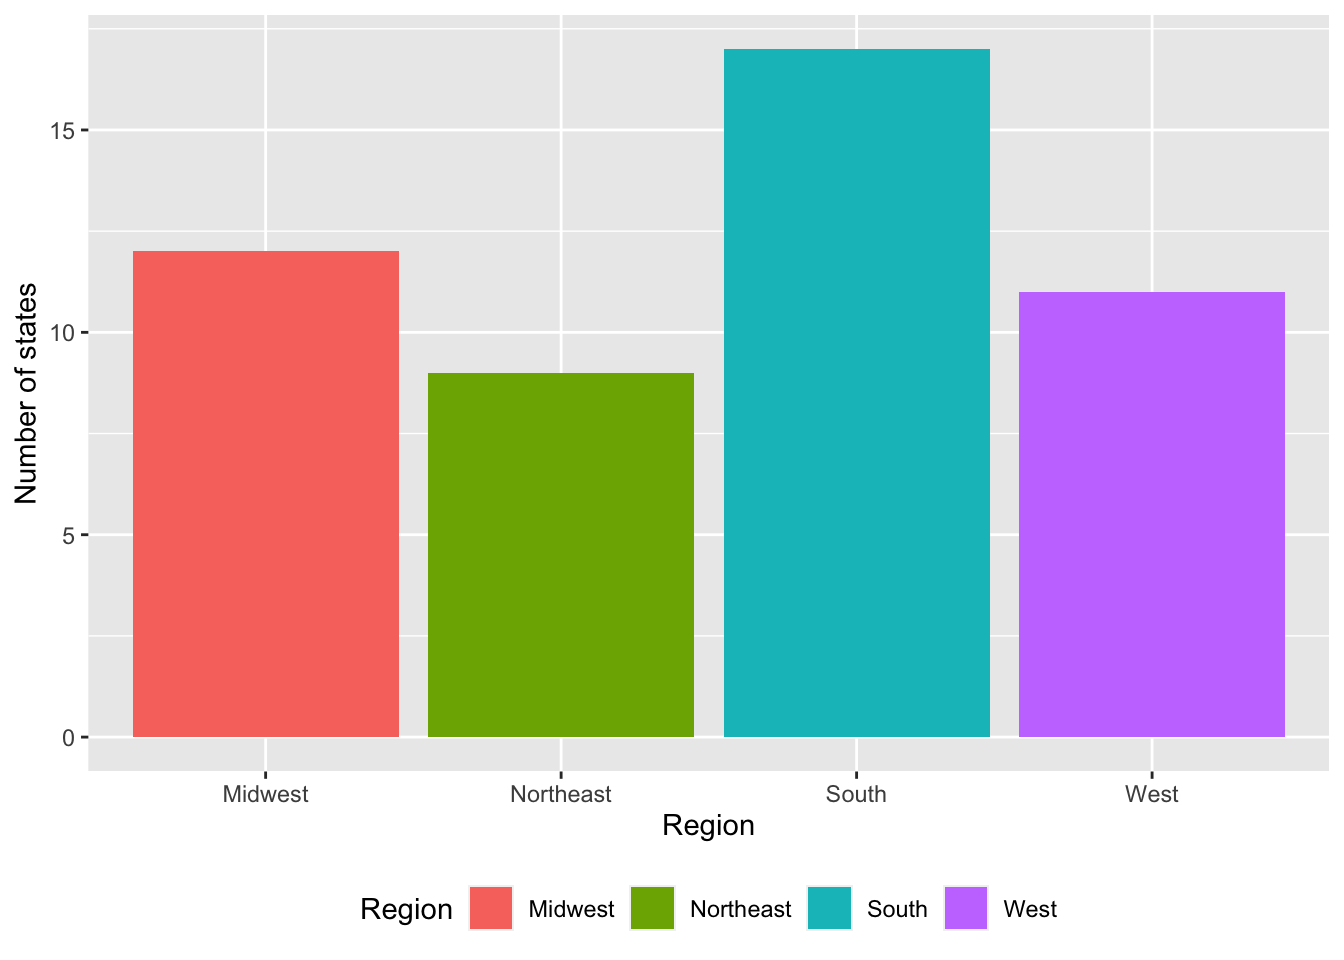
\includegraphics[width=0.5\linewidth]{bookdown-demo_files/figure-latex/unnamed-chunk-49-1} 

}

\caption{Scatterplot with legend at bottom}\label{fig:unnamed-chunk-49}
\end{figure}

\begin{enumerate}
\def\labelenumi{\arabic{enumi}.}
\setcounter{enumi}{1}
\tightlist
\item
  Legend guide \texttt{guide\_legend()}
\end{enumerate}

We can also assign individual keys to the legend using options of
\texttt{guide\_legend()}. Here we introduce the most useful options.

\begin{itemize}
\tightlist
\item
  \texttt{nrow} and \texttt{ncol}: specify the dimensions of the table.
  \texttt{byrow}: fills the rows, set to \texttt{FALSE} by default.
\end{itemize}

\begin{Shaded}
\begin{Highlighting}[]
\NormalTok{p }\OperatorTok{+}\StringTok{ }\KeywordTok{guides}\NormalTok{(}\DataTypeTok{fill =} \KeywordTok{guide_legend}\NormalTok{(}\DataTypeTok{ncol =} \DecValTok{2}\NormalTok{, }\DataTypeTok{byrow =} \OtherTok{TRUE}\NormalTok{))}
\end{Highlighting}
\end{Shaded}

\begin{figure}

{\centering 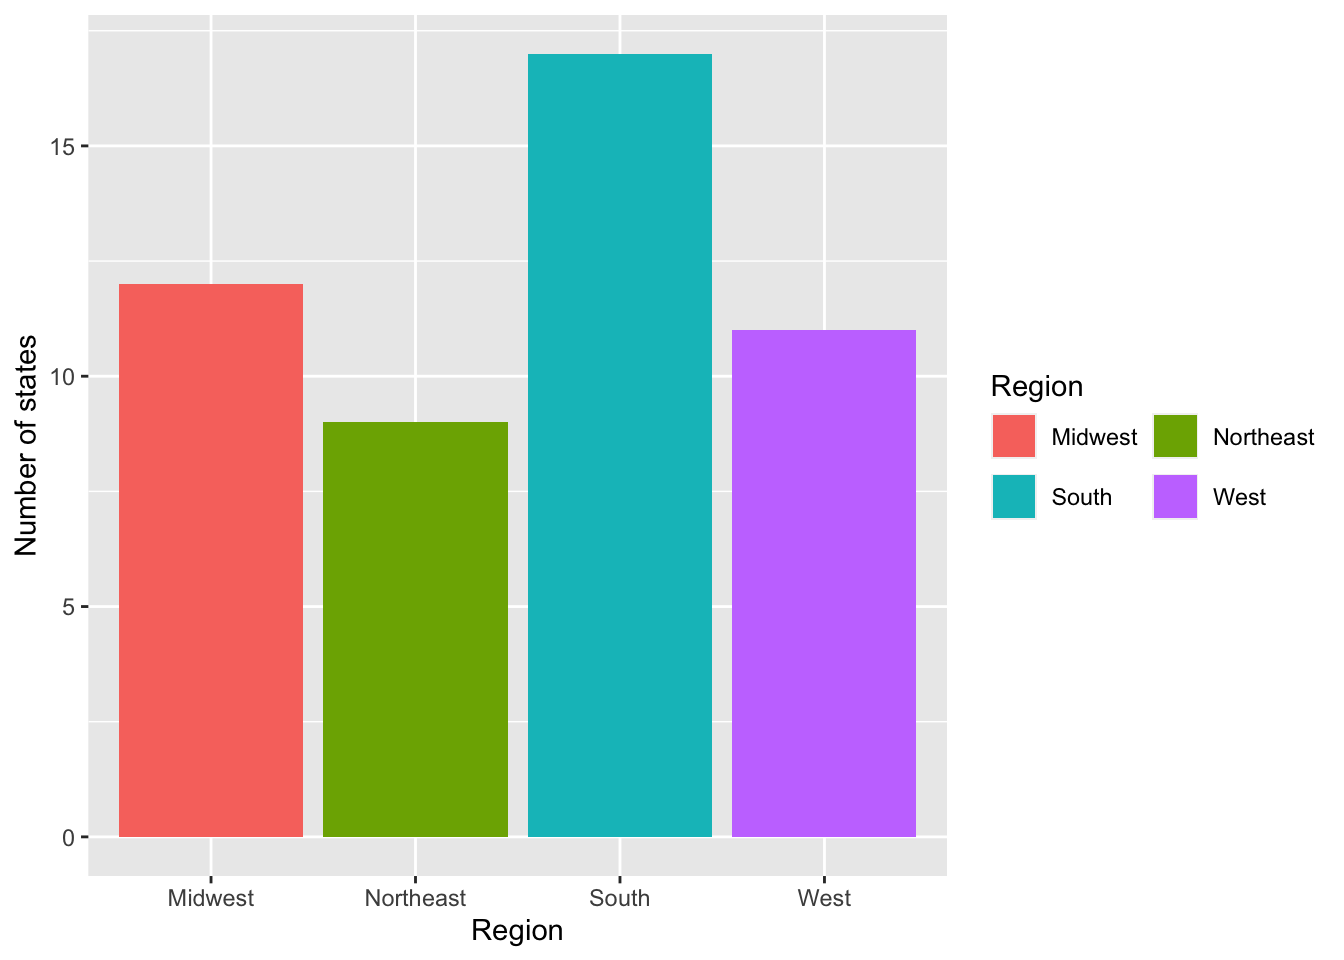
\includegraphics[width=0.5\linewidth]{bookdown-demo_files/figure-latex/unnamed-chunk-50-1} 

}

\caption{Bar plots of number of states in each region}\label{fig:unnamed-chunk-50}
\end{figure}

\begin{itemize}
\tightlist
\item
  \texttt{reverse}: reverse the order of the keys
\end{itemize}

\begin{Shaded}
\begin{Highlighting}[]
\NormalTok{p }\OperatorTok{+}\StringTok{ }\KeywordTok{guides}\NormalTok{(}\DataTypeTok{fill =} \KeywordTok{guide_legend}\NormalTok{(}\DataTypeTok{reverse =} \OtherTok{TRUE}\NormalTok{))}
\end{Highlighting}
\end{Shaded}

\begin{figure}

{\centering 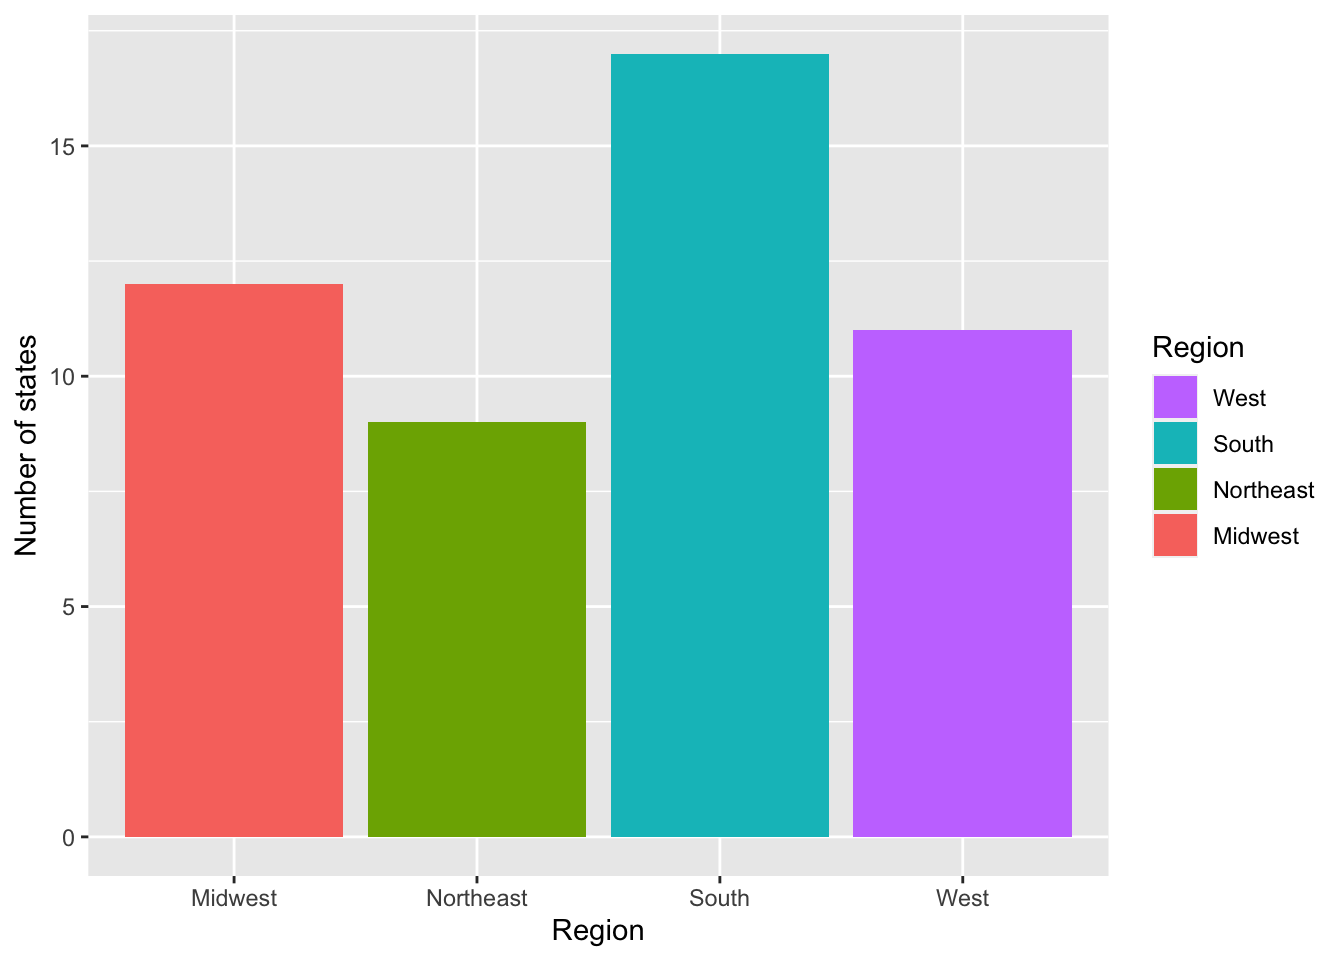
\includegraphics[width=0.5\linewidth]{bookdown-demo_files/figure-latex/unnamed-chunk-51-1} 

}

\caption{Bar plots of number of states in each region}\label{fig:unnamed-chunk-51}
\end{figure}

\subsection{Boxplots, jittering and violin
plots}\label{boxplots-jittering-and-violin-plots}

Conditioning on a categorical feature, or conditioning on groups, we may
want to conduct a side-by-side comparison for a certain variable. We can
use the following tools.

\begin{quote}
\begin{itemize}
\tightlist
\item
  Jittering, \texttt{geom\_jitter()}, adds a little random noise to the
  data, which can help avoid overplotting.
\item
  Boxplots, \texttt{geom\_boxplot()}, summarize the shape of the
  distribution with a handful of summary statistics.
\item
  Violin plots, \texttt{geom\_violin()}, show a compact representation
  of the ``density'' of the distribution, highlighting the areas where
  more points are found.
\end{itemize}
\end{quote}

\begin{Shaded}
\begin{Highlighting}[]
\NormalTok{df <-}\StringTok{ }\NormalTok{slid}\OperatorTok{::}\NormalTok{state.long }\OperatorTok\StringTok{ }
\StringTok{  }\NormalTok{dplyr}\OperatorTok{::}\KeywordTok{filter}\NormalTok{(DATE }\OperatorTok{==}\StringTok{ }\KeywordTok{as.Date}\NormalTok{(}\StringTok{'2020-12-11'}\NormalTok{)) }\OperatorTok
\StringTok{  }\KeywordTok{mutate}\NormalTok{(}\DataTypeTok{Risk =}\NormalTok{ Infected }\OperatorTok{/}\StringTok{ }\NormalTok{pop)}

\NormalTok{p <-}\StringTok{ }\KeywordTok{ggplot}\NormalTok{(df, }\KeywordTok{aes}\NormalTok{(Region, Risk, }\DataTypeTok{color =}\NormalTok{ Region)) }
\NormalTok{p }\OperatorTok{+}\StringTok{ }\KeywordTok{geom_point}\NormalTok{()}
\NormalTok{p }\OperatorTok{+}\StringTok{ }\KeywordTok{geom_jitter}\NormalTok{()}
\NormalTok{p }\OperatorTok{+}\StringTok{ }\KeywordTok{geom_boxplot}\NormalTok{()}
\NormalTok{p }\OperatorTok{+}\StringTok{ }\KeywordTok{geom_violin}\NormalTok{()}
\end{Highlighting}
\end{Shaded}

\begin{figure}
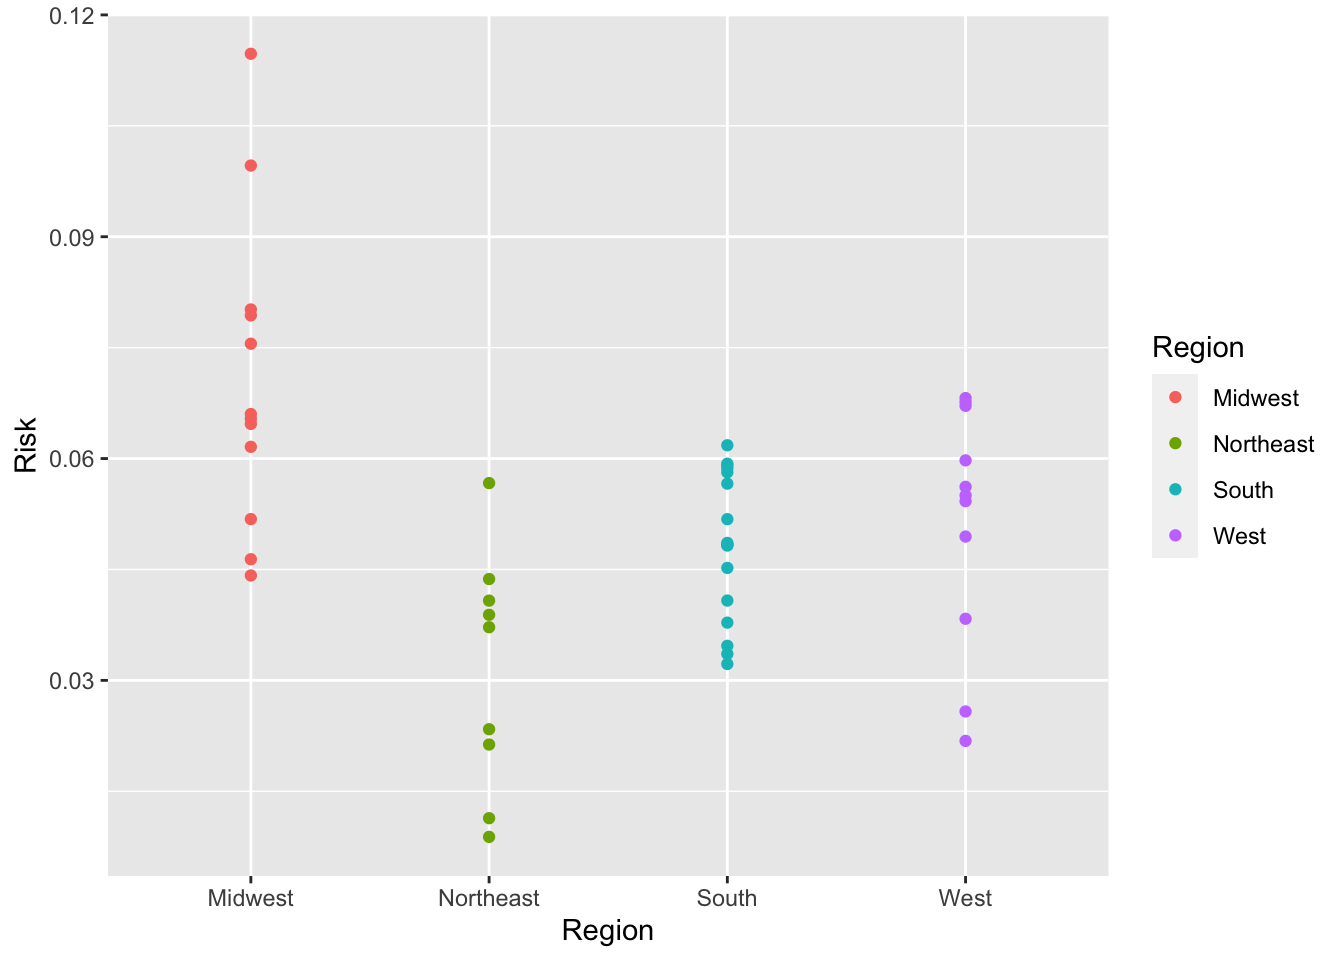
\includegraphics[width=0.5\linewidth]{bookdown-demo_files/figure-latex/Boxplot3-1} 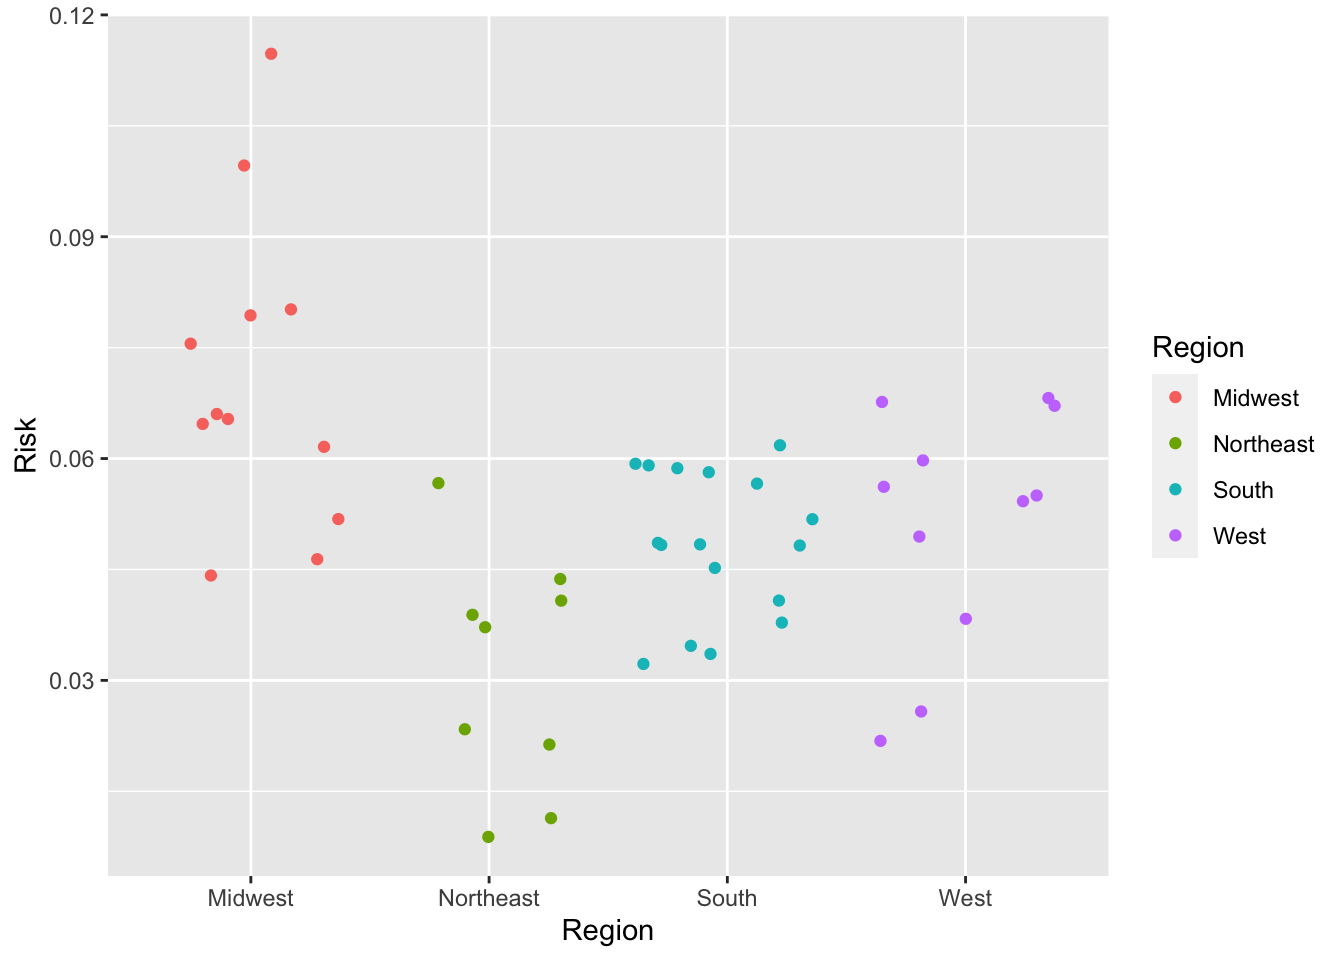
\includegraphics[width=0.5\linewidth]{bookdown-demo_files/figure-latex/Boxplot3-2} 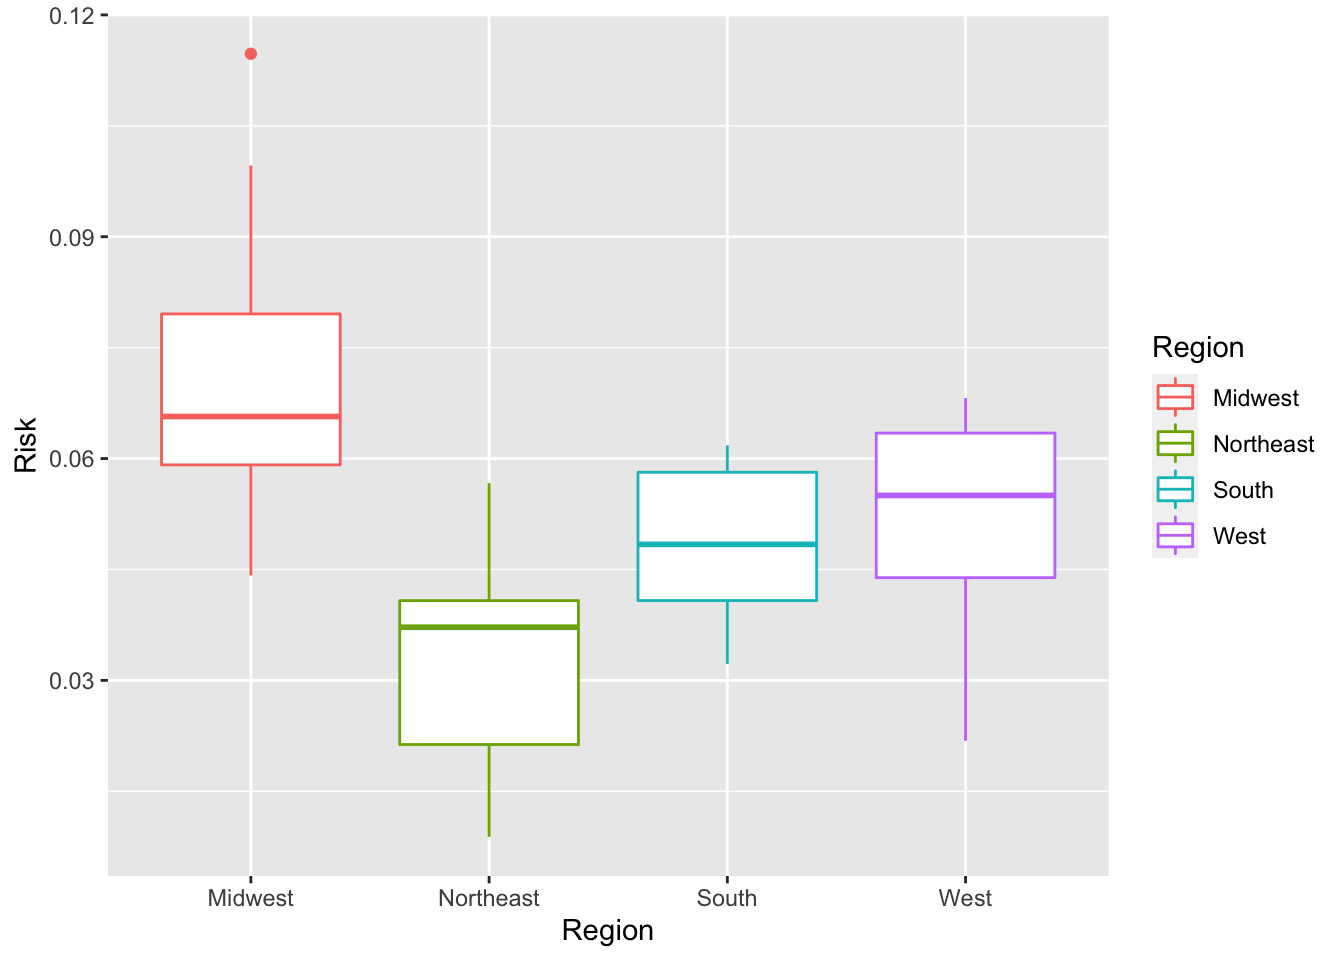
\includegraphics[width=0.5\linewidth]{bookdown-demo_files/figure-latex/Boxplot3-3} 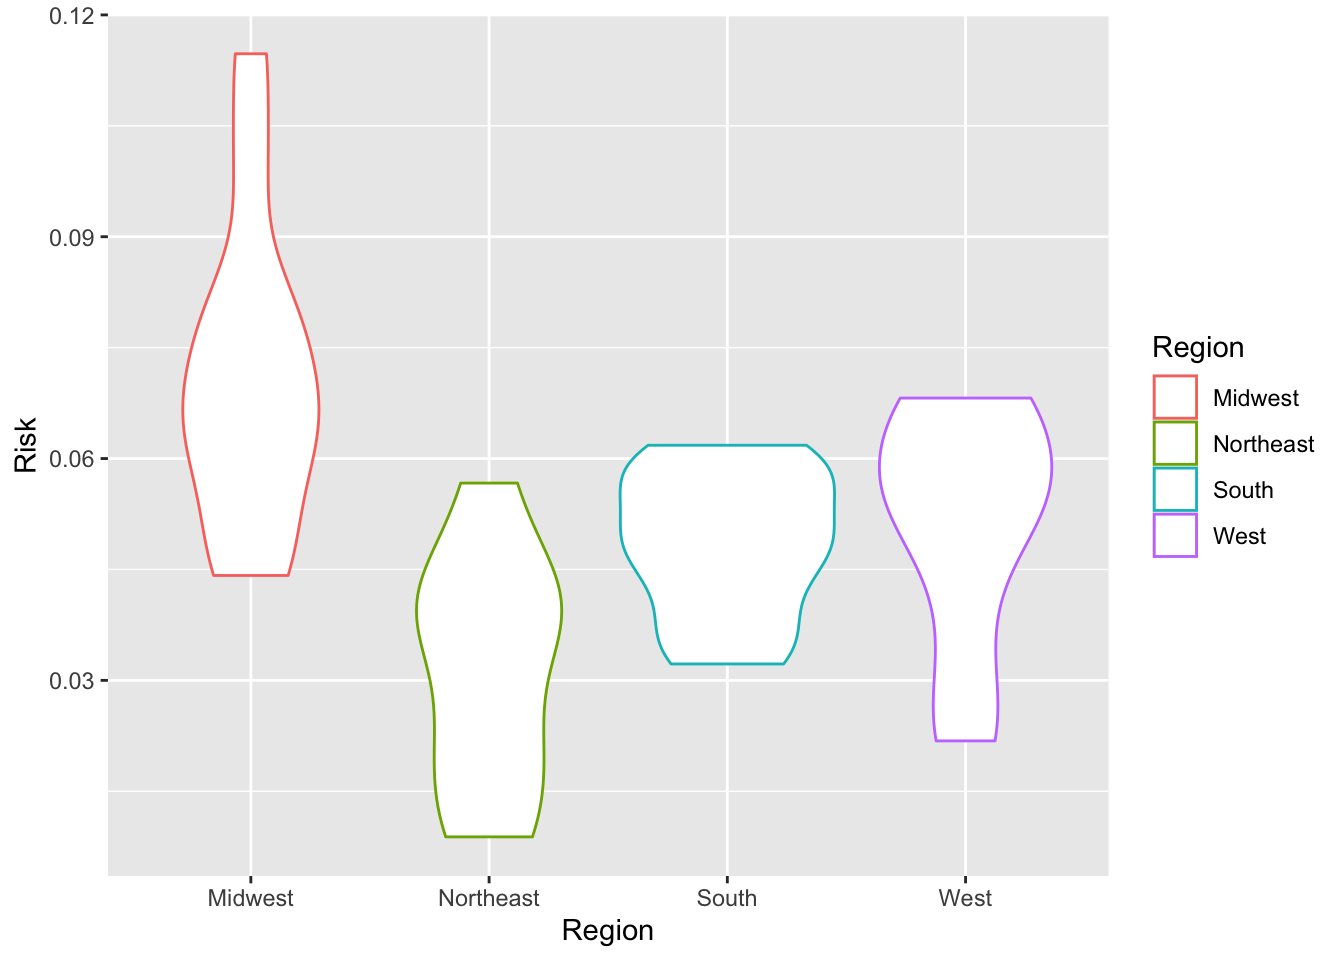
\includegraphics[width=0.5\linewidth]{bookdown-demo_files/figure-latex/Boxplot3-4} \caption{Points, jittering, boxplot, and violin plot examples}\label{fig:Boxplot3}
\end{figure}

\section{Collective geoms}\label{collective-geoms}

An individual ``geom'' draws a distinct graphical object for each
observation (row). For example, the ``point geom'' draws one point per
row. Several geoms can be added to the same ggplot object, which allows
you to build up layers to create complex graphs and displays multiple
observations with one geometric object. For example, we previously have
created a scatter plot, and we can add regressed lines on the top of the
scatter plot layer. You can add more information from a statistical
summary, or add a text geom to annotate your plot.

\subsection{Smoother}\label{smoother}

On top of the scatter plot, we can add regressed lines and prediction
band to it using \texttt{geom\_smooth()}.

\begin{enumerate}
\def\labelenumi{\arabic{enumi}.}
\tightlist
\item
  The ``loess'' method
\end{enumerate}

By default, the model for small data is ``loess'', we can call the layer
either by \texttt{geom\_smooth()} or
\texttt{geom\_smooth(method\ =\textquotesingle{}loess\textquotesingle{})}.
In addition, we can adjust option \texttt{span} to control the
wiggliness of the line. The higher \texttt{span} is, the less wiggle the
line will be.

\begin{Shaded}
\begin{Highlighting}[]
\NormalTok{df <-}\StringTok{ }\NormalTok{slid}\OperatorTok{::}\NormalTok{state.long }\OperatorTok\StringTok{ }
\StringTok{  }\NormalTok{dplyr}\OperatorTok{::}\KeywordTok{filter}\NormalTok{(DATE }\OperatorTok{==}\StringTok{ }\KeywordTok{as.Date}\NormalTok{(}\StringTok{'2020-12-11'}\NormalTok{)) }
\NormalTok{p <-}\StringTok{ }\KeywordTok{ggplot}\NormalTok{(df, }\KeywordTok{aes}\NormalTok{(}\KeywordTok{log}\NormalTok{(Infected }\OperatorTok{+}\StringTok{ }\DecValTok{1}\NormalTok{), }\KeywordTok{log}\NormalTok{(Death }\OperatorTok{+}\StringTok{ }\DecValTok{1}\NormalTok{))) }\OperatorTok{+}
\StringTok{  }\KeywordTok{geom_point}\NormalTok{()}
\CommentTok{# Use `span` to control the wiggliness of the line}
\CommentTok{# The higher `span` is, the less wiggle the line is}
\NormalTok{p }\OperatorTok{+}\StringTok{ }\KeywordTok{geom_smooth}\NormalTok{(}\DataTypeTok{method =} \StringTok{'loess'}\NormalTok{, }\DataTypeTok{span =} \FloatTok{0.5}\NormalTok{) }
\NormalTok{p }\OperatorTok{+}\StringTok{ }\KeywordTok{geom_smooth}\NormalTok{(}\DataTypeTok{method =} \StringTok{'loess'}\NormalTok{, }\DataTypeTok{span =} \DecValTok{1}\NormalTok{) }
\end{Highlighting}
\end{Shaded}

\begin{figure}
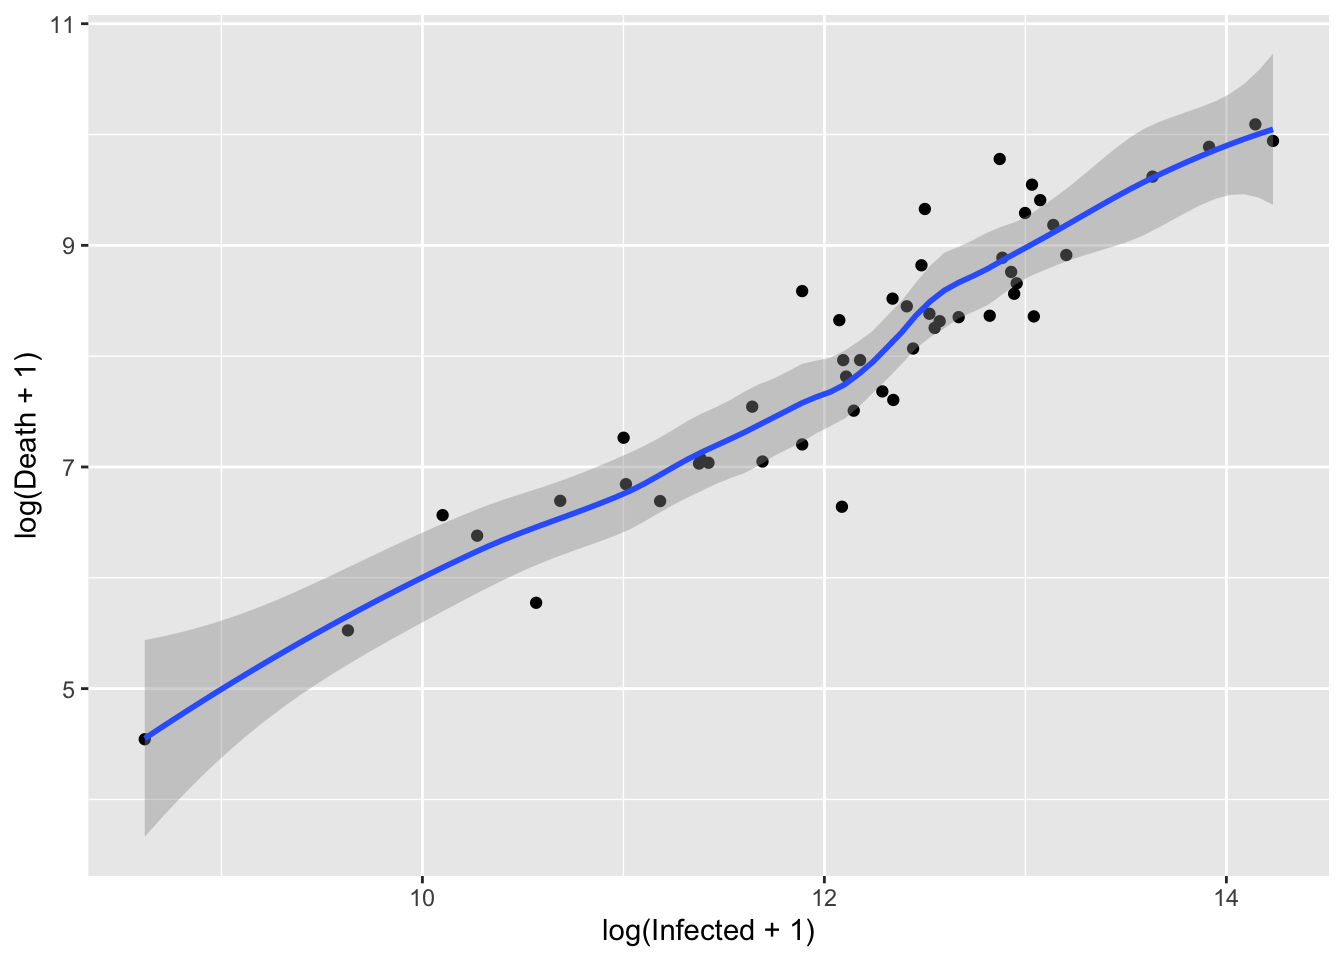
\includegraphics[width=0.5\linewidth]{bookdown-demo_files/figure-latex/unnamed-chunk-52-1} 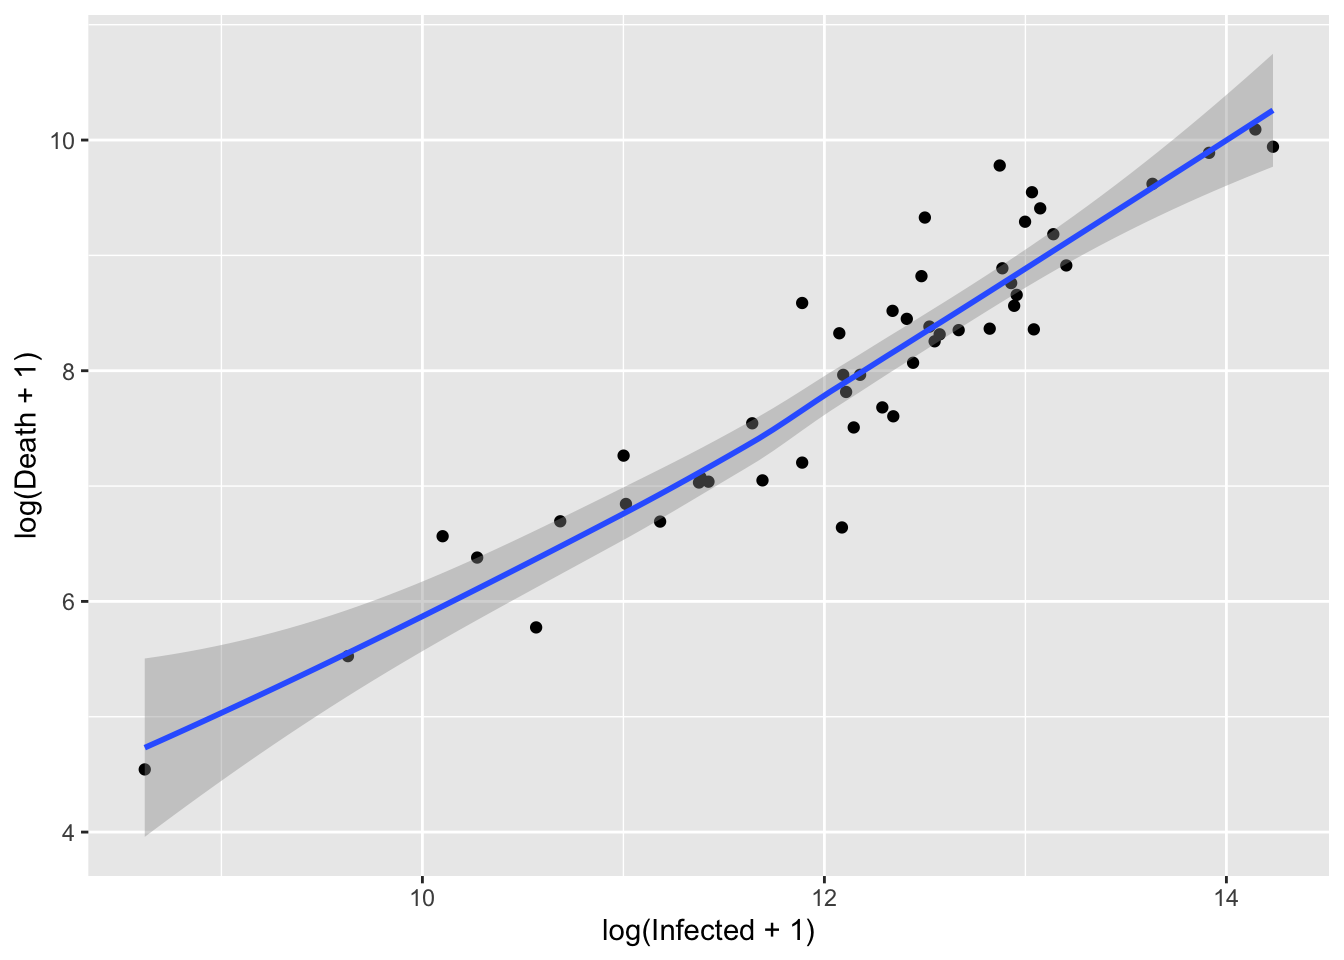
\includegraphics[width=0.5\linewidth]{bookdown-demo_files/figure-latex/unnamed-chunk-52-2} \caption{loess smoother examples}\label{fig:unnamed-chunk-52}
\end{figure}

\begin{enumerate}
\def\labelenumi{\arabic{enumi}.}
\setcounter{enumi}{1}
\tightlist
\item
  Linear regression method
\end{enumerate}

We can also use
\texttt{method\ =\ \textquotesingle{}lm\textquotesingle{}} to fit a
simple linear model:

\begin{Shaded}
\begin{Highlighting}[]
\CommentTok{# Fit a linear model}
\NormalTok{p }\OperatorTok{+}\StringTok{ }\KeywordTok{geom_smooth}\NormalTok{(}\DataTypeTok{method =} \StringTok{'lm'}\NormalTok{)  }
\end{Highlighting}
\end{Shaded}

\begin{figure}
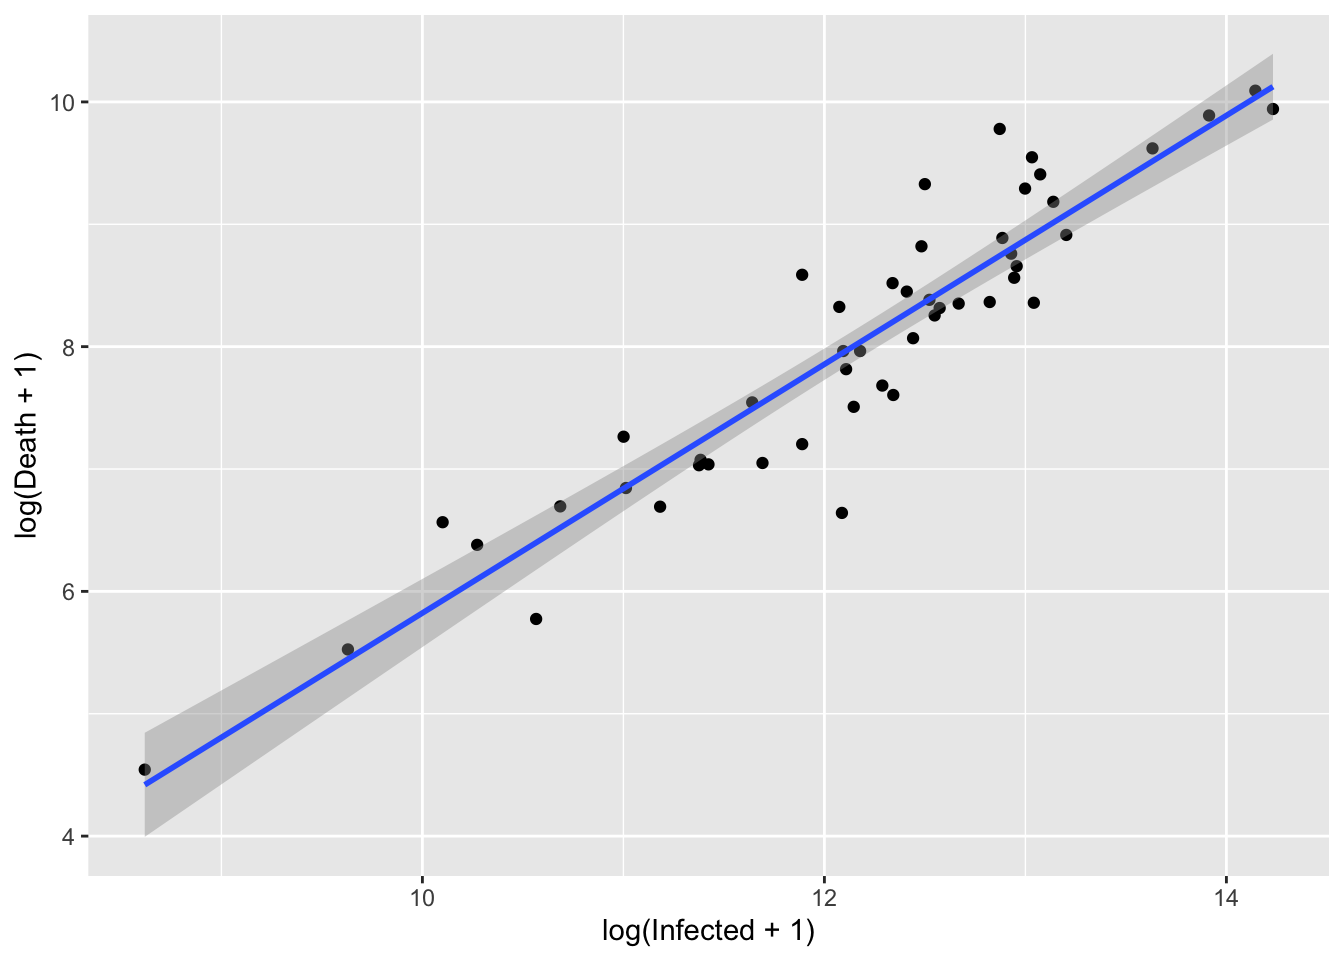
\includegraphics[width=0.5\linewidth]{bookdown-demo_files/figure-latex/unnamed-chunk-53-1} \caption{Linear regression estimator.}\label{fig:unnamed-chunk-53}
\end{figure}

After introducing the idea of individual and collective geoms, we would
like to spend the rest of the chapter discussing two important
collective plots, time series plots and maps. We will build them step by
step from scratch.

\section{Time Series}\label{time-series}

\subsection{Basic line plots}\label{basic-line-plots}

In traditional time series plots, we use time as the x-axis variable,
and plot the time series using \texttt{geom\_line()}.

We consider the time series of the daily new infected count for Iowa.

\begin{Shaded}
\begin{Highlighting}[]
\NormalTok{df <-}\StringTok{ }\NormalTok{slid}\OperatorTok{::}\NormalTok{state.long }\OperatorTok
\StringTok{  }\NormalTok{dplyr}\OperatorTok{::}\KeywordTok{filter}\NormalTok{(State }\OperatorTok{==}\StringTok{ "Iowa"}\NormalTok{) }\OperatorTok
\StringTok{  }\KeywordTok{arrange}\NormalTok{(DATE) }\OperatorTok
\StringTok{  }\KeywordTok{mutate}\NormalTok{(}\DataTypeTok{Y.Infected =}\NormalTok{ Infected }\OperatorTok{-}\StringTok{ }\KeywordTok{lag}\NormalTok{(Infected)) }\OperatorTok
\StringTok{  }\NormalTok{dplyr}\OperatorTok{::}\KeywordTok{filter}\NormalTok{(}\OperatorTok{!}\KeywordTok{is.na}\NormalTok{(Y.Infected))}
\end{Highlighting}
\end{Shaded}

To visualize the data, we draw a time series plot first.

\begin{Shaded}
\begin{Highlighting}[]
\NormalTok{p <-}\StringTok{ }\KeywordTok{ggplot}\NormalTok{(df, }\KeywordTok{aes}\NormalTok{(DATE, Y.Infected)) }\OperatorTok{+}\StringTok{ }
\StringTok{  }\KeywordTok{geom_line}\NormalTok{() }\OperatorTok{+}\StringTok{ }
\StringTok{  }\KeywordTok{labs}\NormalTok{(}\DataTypeTok{x =} \StringTok{"Days"}\NormalTok{, }\DataTypeTok{y =} \StringTok{"Count"}\NormalTok{, }
       \DataTypeTok{title =} \StringTok{'Daily new infected cases in Iowa'}\NormalTok{) }
\NormalTok{p}
\end{Highlighting}
\end{Shaded}

\begin{figure}

{\centering 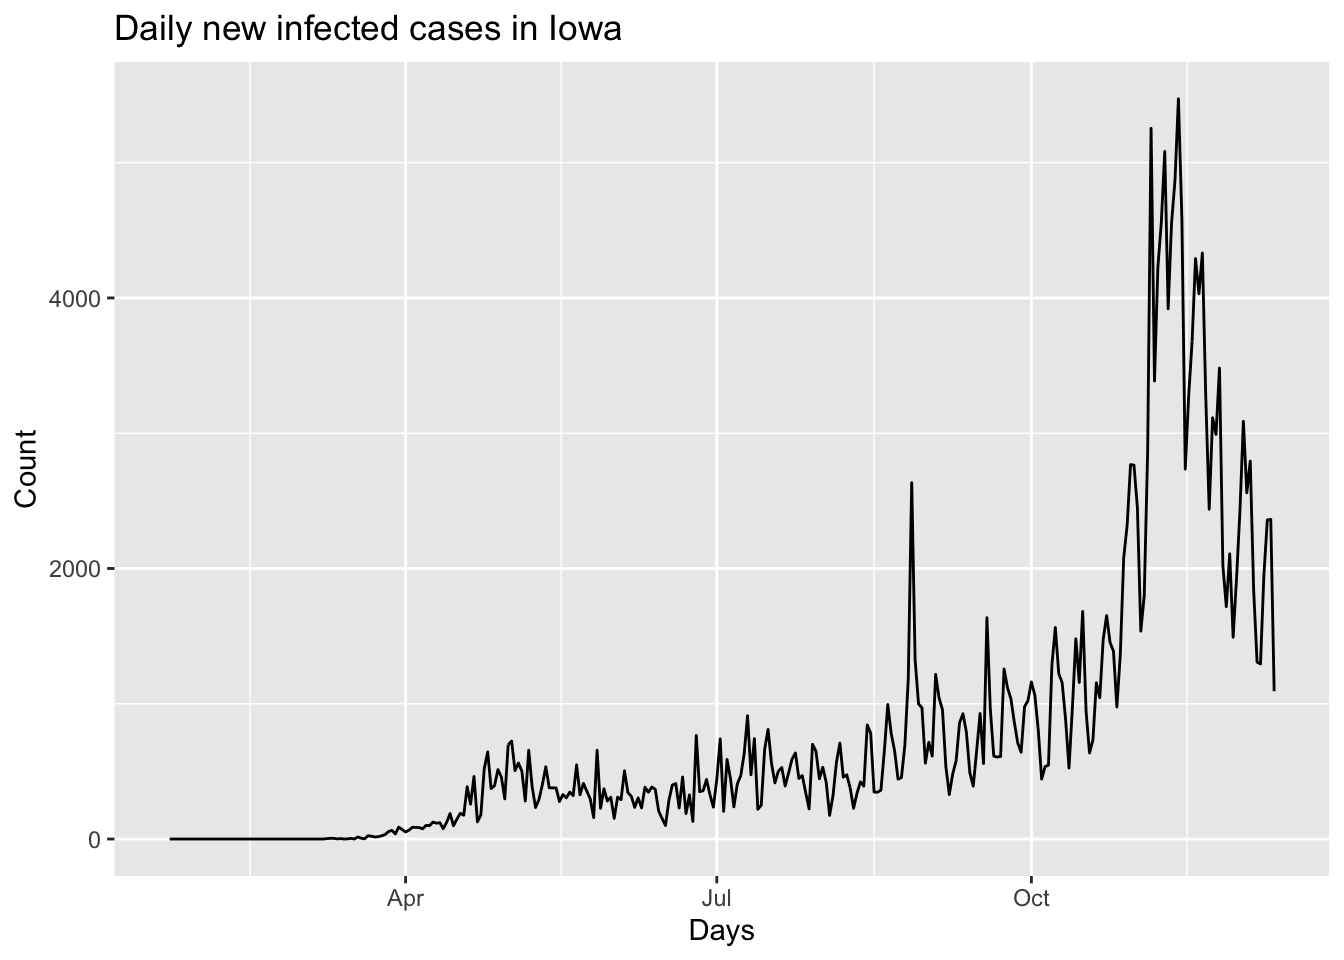
\includegraphics[width=0.8\linewidth]{bookdown-demo_files/figure-latex/Timeseries2-1} 

}

\caption{Basic time series}\label{fig:Timeseries2}
\end{figure}

\subsection{Add a second line}\label{add-a-second-line}

Next, we display the prediction results on the time series plot. The
prediction and prediction intervals for the next 14 days are saved in
the dataset: \texttt{slid::fore}.

\begin{Shaded}
\begin{Highlighting}[]
\CommentTok{# Data Preparation}
\ControlFlowTok{if}\NormalTok{(}\OperatorTok{!}\KeywordTok{require}\NormalTok{(}\StringTok{'lubridate'}\NormalTok{)) }\KeywordTok{install.packages}\NormalTok{(}\StringTok{'lubridate'}\NormalTok{)}
\end{Highlighting}
\end{Shaded}

\begin{Shaded}
\begin{Highlighting}[]
\KeywordTok{library}\NormalTok{(lubridate)}
\NormalTok{df.pred <-}\StringTok{ }\KeywordTok{as.data.frame}\NormalTok{(slid}\OperatorTok{::}\NormalTok{fore[}\KeywordTok{c}\NormalTok{(}\StringTok{'mean'}\NormalTok{, }\StringTok{'lower'}\NormalTok{, }\StringTok{'upper'}\NormalTok{)])}
\KeywordTok{names}\NormalTok{(df.pred) <-}\StringTok{ }\KeywordTok{c}\NormalTok{(}\StringTok{'mean'}\NormalTok{, }\StringTok{'lower'}\NormalTok{, }\StringTok{'upper'}\NormalTok{)}
\NormalTok{df.pred}\OperatorTok{$}\NormalTok{DATE <-}\StringTok{ }\KeywordTok{tail}\NormalTok{(df}\OperatorTok{$}\NormalTok{DATE,}\DecValTok{1}\NormalTok{) }\OperatorTok{+}\StringTok{ }
\StringTok{  }\KeywordTok{c}\NormalTok{(}\DecValTok{1}\OperatorTok{:}\KeywordTok{length}\NormalTok{(slid}\OperatorTok{::}\NormalTok{fore}\OperatorTok{$}\NormalTok{mean))}
\end{Highlighting}
\end{Shaded}

\begin{Shaded}
\begin{Highlighting}[]
\CommentTok{# Add a line for predicted value}
\NormalTok{p }\OperatorTok{+}\StringTok{ }\KeywordTok{geom_line}\NormalTok{(}\DataTypeTok{mapping =} \KeywordTok{aes}\NormalTok{(}\DataTypeTok{x =}\NormalTok{ DATE, }
                            \DataTypeTok{y =}\NormalTok{ mean,}
                            \DataTypeTok{color =} \StringTok{'Predicted Value'}\NormalTok{),}
              \DataTypeTok{linetype =} \StringTok{"dashed"}\NormalTok{,}
              \CommentTok{# Set the line type in legend}
              \DataTypeTok{key_glyph =} \StringTok{"timeseries"}\NormalTok{,}
              \DataTypeTok{data =}\NormalTok{ df.pred) }\OperatorTok{+}\StringTok{ }
\StringTok{  }\KeywordTok{scale_color_manual}\NormalTok{(}\StringTok{""}\NormalTok{, }\DataTypeTok{values =} \StringTok{"red"}\NormalTok{)}
\end{Highlighting}
\end{Shaded}

\begin{figure}

{\centering 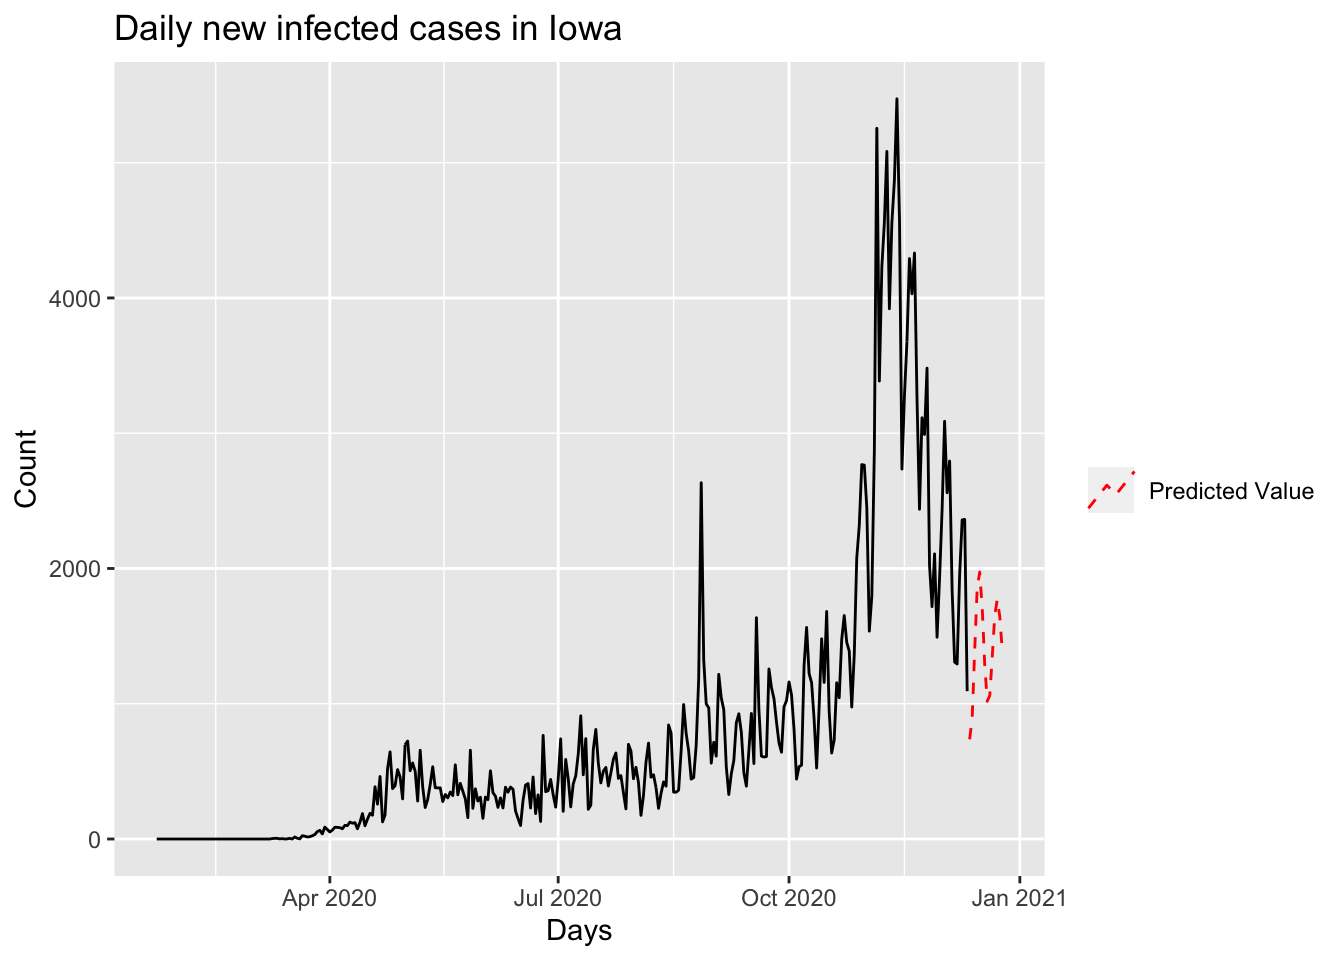
\includegraphics[width=1\linewidth]{bookdown-demo_files/figure-latex/tspred0-1} 

}

\caption{Time series with added predictions}\label{fig:tspred0}
\end{figure}

\subsection{Add ribbons}\label{add-ribbons}

Next, we show the prediction intervals. On top of the line plots, we can
add another layer to the existing line, and create a line with two
parts.

\begin{Shaded}
\begin{Highlighting}[]
\CommentTok{# Add prediction intervals}
\NormalTok{p <-}\StringTok{ }\NormalTok{p }\OperatorTok{+}\StringTok{ }
\StringTok{  }\KeywordTok{geom_ribbon}\NormalTok{(}\DataTypeTok{mapping =} \KeywordTok{aes}\NormalTok{(}\DataTypeTok{x =}\NormalTok{ DATE, }
                            \DataTypeTok{y =}\NormalTok{ mean, }
                            \DataTypeTok{ymin =}\NormalTok{ lower, }
                            \DataTypeTok{ymax =}\NormalTok{ upper,}
                            \DataTypeTok{fill =} \StringTok{'95% Prediction Intervals'}\NormalTok{), }
              \DataTypeTok{data =}\NormalTok{ df.pred, }\DataTypeTok{alpha =} \FloatTok{0.2}\NormalTok{) }\OperatorTok{+}\StringTok{ }
\CommentTok{# Add line for predicted value}
\KeywordTok{geom_line}\NormalTok{(}\DataTypeTok{mapping =} \KeywordTok{aes}\NormalTok{(}\DataTypeTok{x =}\NormalTok{ DATE,}
\DataTypeTok{y =}\NormalTok{ mean,}
\DataTypeTok{color =} \StringTok{'Predicted Value'}\NormalTok{),}
\DataTypeTok{linetype =} \StringTok{"dashed"}\NormalTok{, }\DataTypeTok{data =}\NormalTok{ df.pred,}
\CommentTok{# Set the line type in legend}
\DataTypeTok{key_glyph =} \StringTok{"timeseries"}\NormalTok{) }\OperatorTok{+}
\KeywordTok{scale_color_manual}\NormalTok{(}\StringTok{""}\NormalTok{, }\DataTypeTok{values =} \StringTok{"red"}\NormalTok{)}\OperatorTok{+}
\KeywordTok{scale_fill_manual}\NormalTok{(}\StringTok{""}\NormalTok{, }\DataTypeTok{values =} \StringTok{"pink"}\NormalTok{)}

\NormalTok{p}
\end{Highlighting}
\end{Shaded}

\begin{figure}

{\centering 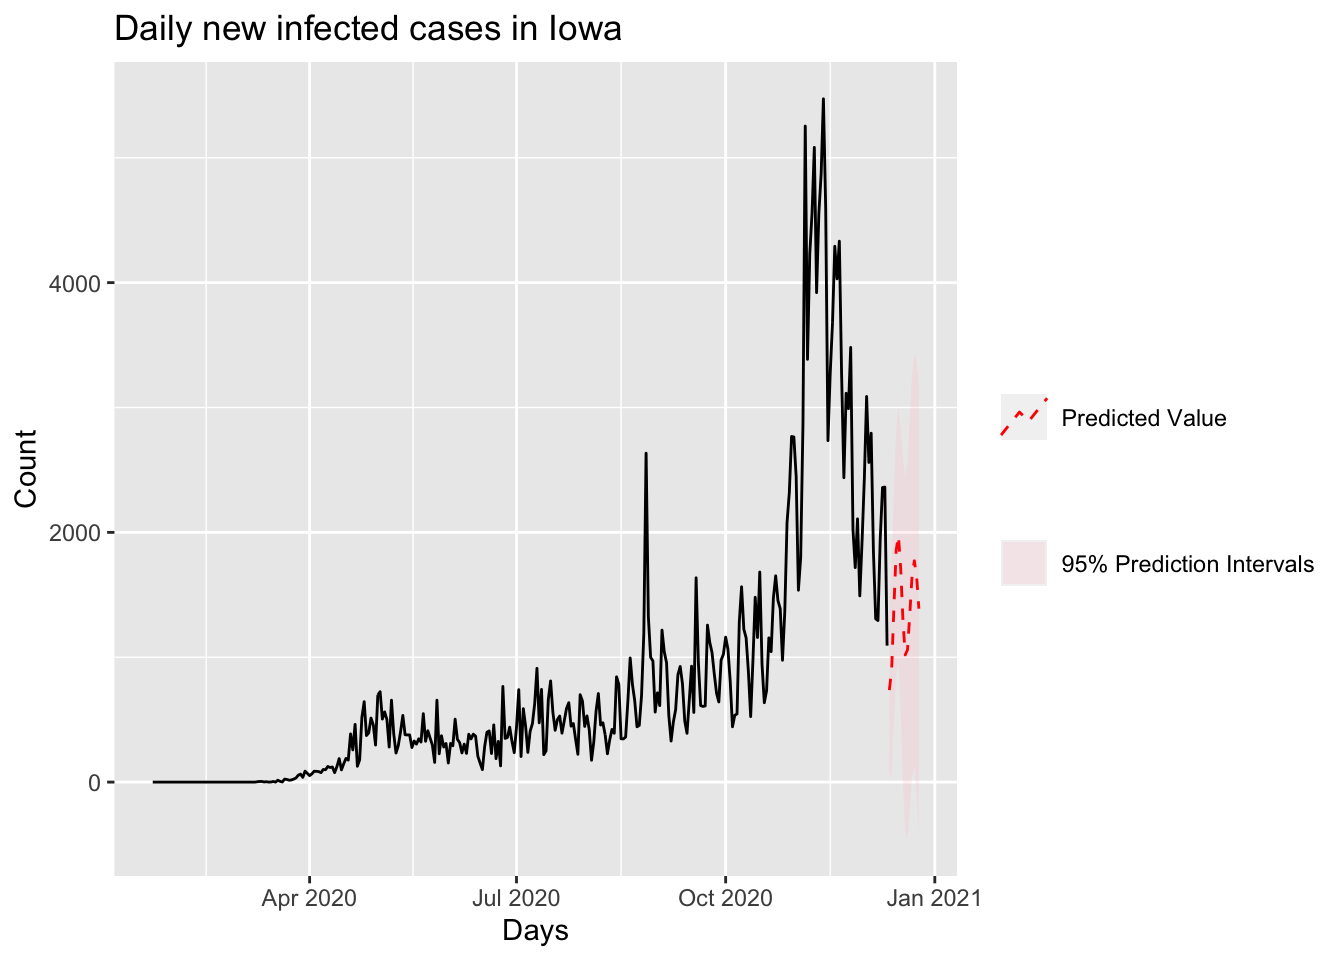
\includegraphics[width=1\linewidth]{bookdown-demo_files/figure-latex/tspred-1} 

}

\caption{Time series with ribbons and second line}\label{fig:tspred}
\end{figure}

\textbf{Remarks:} the layer added later is put on the top, therefore it
is important to keep track of the order you add the layers.

\subsection{Adjust the scale of time
axis}\label{adjust-the-scale-of-time-axis}

There are several ways to define the axis ticks of dates and times.
There are the labeled \textbf{major breaks} and further the
\textbf{minor breaks}, which are not labeled but marked by grid lines.
These can be customized with the arguments \texttt{date\_breaks} and
\texttt{date\_minor\_breaks}, respectively.

\begin{Shaded}
\begin{Highlighting}[]
\CommentTok{# Adjust the scale of time axis}
\NormalTok{p }\OperatorTok{+}\StringTok{ }\KeywordTok{scale_x_date}\NormalTok{(}
  \DataTypeTok{limits =} \KeywordTok{as.Date}\NormalTok{(}\KeywordTok{c}\NormalTok{(}\StringTok{"2020-10-01"}\NormalTok{, }\StringTok{"2021-01-01"}\NormalTok{)),}
  \DataTypeTok{date_breaks =} \StringTok{"1 month"}\NormalTok{,}
  \DataTypeTok{date_minor_breaks =} \StringTok{"1 week"}\NormalTok{,}
  \DataTypeTok{date_labels =} \StringTok{"%B %Y"}
\NormalTok{)}
\end{Highlighting}
\end{Shaded}

\begin{figure}

{\centering 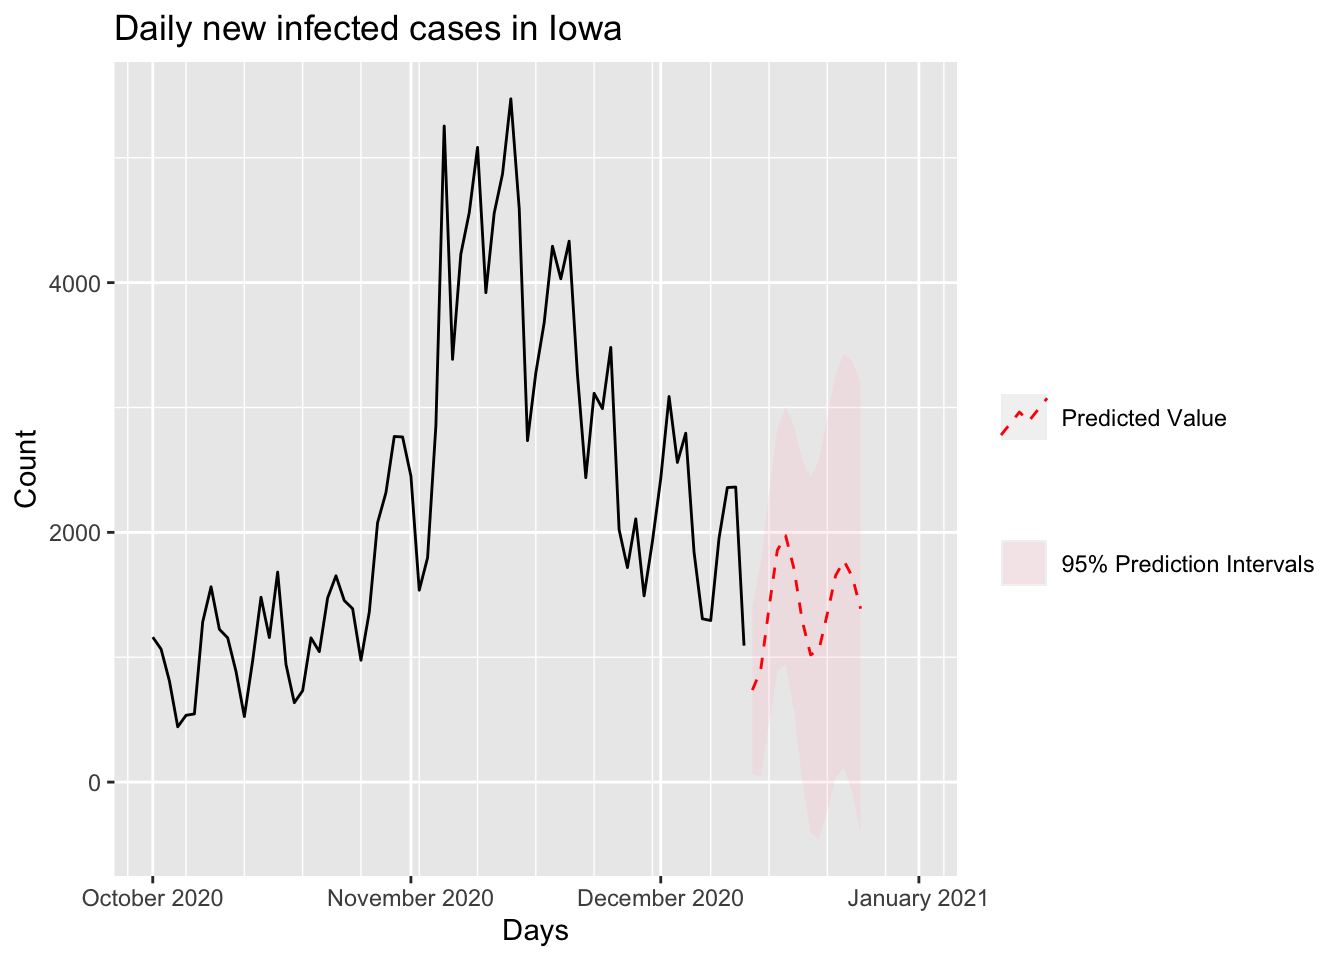
\includegraphics[width=1\linewidth]{bookdown-demo_files/figure-latex/unnamed-chunk-57-1} 

}

\caption{Time series plot with adjusted time range and format}\label{fig:unnamed-chunk-57}
\end{figure}

In the above syntax, \texttt{date\_labels} set to a string of formatting
codes, defining order, format and elements to be displayed:

\begin{itemize}
\tightlist
\item
  \texttt{\%d}: day of the month (01-31)
\item
  \texttt{\%m}: month, numeric (01-12)
\item
  \texttt{\%b}: month, abbreviated (Jan-Dec)
\item
  \texttt{\%B}: month, full (January-December)
\item
  \texttt{\%y}: year, without century (00-99)
\item
  \texttt{\%Y}: year, with century (0000-9999)
\end{itemize}

\subsection{Add annotations}\label{add-annotations}

When constructing a data visualization, it is often necessary to make
annotations to the data displayed. An annotation supplies additional
information about the data being displayed. For example, adding text to
a plot is one of the most common forms of annotation. The primary tool
for labeling plots is \texttt{geom\_text()}, which adds label text at
the specified \texttt{x} and \texttt{y} positions. We can also add
reference lines to the plot using \texttt{geom\_vline} or
\texttt{geom\_hline}. Figure \ref{annotate1} shows an annotated time
series plot with shades and reference lines for each quarter.

\begin{Shaded}
\begin{Highlighting}[]
\CommentTok{# Prepare the data}
\NormalTok{df <-}\StringTok{ }\NormalTok{df }\OperatorTok
\StringTok{  }\KeywordTok{mutate}\NormalTok{(}\DataTypeTok{start =} \KeywordTok{floor_date}\NormalTok{(DATE, }\StringTok{"quarter"}\NormalTok{)) }\OperatorTok
\StringTok{  }\KeywordTok{mutate}\NormalTok{(}\DataTypeTok{end =} \KeywordTok{ceiling_date}\NormalTok{(DATE, }\StringTok{"quarter"}\NormalTok{)) }\OperatorTok
\StringTok{  }\KeywordTok{mutate}\NormalTok{(}\DataTypeTok{quarters =} \KeywordTok{as.factor}\NormalTok{(}\KeywordTok{quarter}\NormalTok{(DATE))) }
  
\NormalTok{df.quarters <-}\StringTok{ }\NormalTok{df }\OperatorTok\StringTok{ }
\StringTok{  }\NormalTok{dplyr}\OperatorTok{::}\KeywordTok{select}\NormalTok{(start, end, quarters) }\OperatorTok
\StringTok{  }\KeywordTok{unique}\NormalTok{()}

\CommentTok{# Draw the base ggplot}
\KeywordTok{ggplot}\NormalTok{(df, }\KeywordTok{aes}\NormalTok{(DATE, Y.Infected)) }\OperatorTok{+}
\StringTok{  }\KeywordTok{labs}\NormalTok{(}\DataTypeTok{x =} \StringTok{"Days"}\NormalTok{, }\DataTypeTok{y =} \StringTok{"Count"}\NormalTok{, }
       \DataTypeTok{title =} \StringTok{'Daily new infected cases in Iowa'}\NormalTok{) }\OperatorTok{+}
\StringTok{  }
\StringTok{  }\CommentTok{# Add rectangle for each quarter}
\StringTok{  }\KeywordTok{geom_rect}\NormalTok{(}
    \KeywordTok{aes}\NormalTok{(}\DataTypeTok{xmin =}\NormalTok{ (start), }\DataTypeTok{xmax =}\NormalTok{ (end), }\DataTypeTok{fill =}\NormalTok{ quarters),}
    \DataTypeTok{inherit.aes =}\NormalTok{ F, }\DataTypeTok{ymin =} \OperatorTok{-}\OtherTok{Inf}\NormalTok{, }\DataTypeTok{ymax =} \OtherTok{Inf}\NormalTok{, }
    \DataTypeTok{alpha =}\NormalTok{ .}\DecValTok{5}\NormalTok{, }\DataTypeTok{data =}\NormalTok{ df.quarters) }\OperatorTok{+}\StringTok{ }
\StringTok{  }\KeywordTok{scale_fill_brewer}\NormalTok{(}\DataTypeTok{palette =} \StringTok{"Blues"}\NormalTok{, }\DataTypeTok{aesthetics =} \StringTok{"fill"}\NormalTok{) }\OperatorTok{+}
\StringTok{  }
\StringTok{  }\CommentTok{# Add vertical line}
\StringTok{  }\KeywordTok{geom_vline}\NormalTok{(}\KeywordTok{aes}\NormalTok{(}\DataTypeTok{xintercept =} \KeywordTok{as.numeric}\NormalTok{(start)), }
    \DataTypeTok{data =}\NormalTok{ df, }\DataTypeTok{color =} \StringTok{"gray"}\NormalTok{,}
    \DataTypeTok{linetype =} \StringTok{'dashed'}\NormalTok{, }\DataTypeTok{size =} \FloatTok{0.5}\NormalTok{) }\OperatorTok{+}\StringTok{ }
\StringTok{  }
\StringTok{  }\CommentTok{# Add text}
\StringTok{  }\KeywordTok{geom_text}\NormalTok{(}
    \KeywordTok{aes}\NormalTok{(}\DataTypeTok{x =}\NormalTok{ start, }\DataTypeTok{y =} \DecValTok{0}\NormalTok{ , }\DataTypeTok{label =} \KeywordTok{paste0}\NormalTok{(}\StringTok{'Quarter:'}\NormalTok{, quarters)), }
    \DataTypeTok{data =}\NormalTok{ df.quarters, }\DataTypeTok{inherit.aes =}\NormalTok{ F,}
    \DataTypeTok{size =} \DecValTok{3}\NormalTok{, }\DataTypeTok{vjust =} \DecValTok{0}\NormalTok{, }\DataTypeTok{hjust =} \DecValTok{0}\NormalTok{, }\DataTypeTok{nudge_x =} \DecValTok{20}\NormalTok{) }\OperatorTok{+}
\StringTok{  }
\StringTok{  }\CommentTok{# Add time series lines}
\StringTok{  }\KeywordTok{geom_line}\NormalTok{() }\OperatorTok{+}
\StringTok{  }\KeywordTok{geom_line}\NormalTok{(}\DataTypeTok{mapping =} \KeywordTok{aes}\NormalTok{(}\DataTypeTok{x =}\NormalTok{ DATE, }\DataTypeTok{y =}\NormalTok{ mean,}
                          \DataTypeTok{color =} \StringTok{'Predicted Value'}\NormalTok{),}
            \DataTypeTok{linetype =} \StringTok{"dashed"}\NormalTok{, }\DataTypeTok{data =}\NormalTok{ df.pred ,}
            \DataTypeTok{key_glyph =} \StringTok{"timeseries"}\NormalTok{) }
\end{Highlighting}
\end{Shaded}

\begin{figure}

{\centering 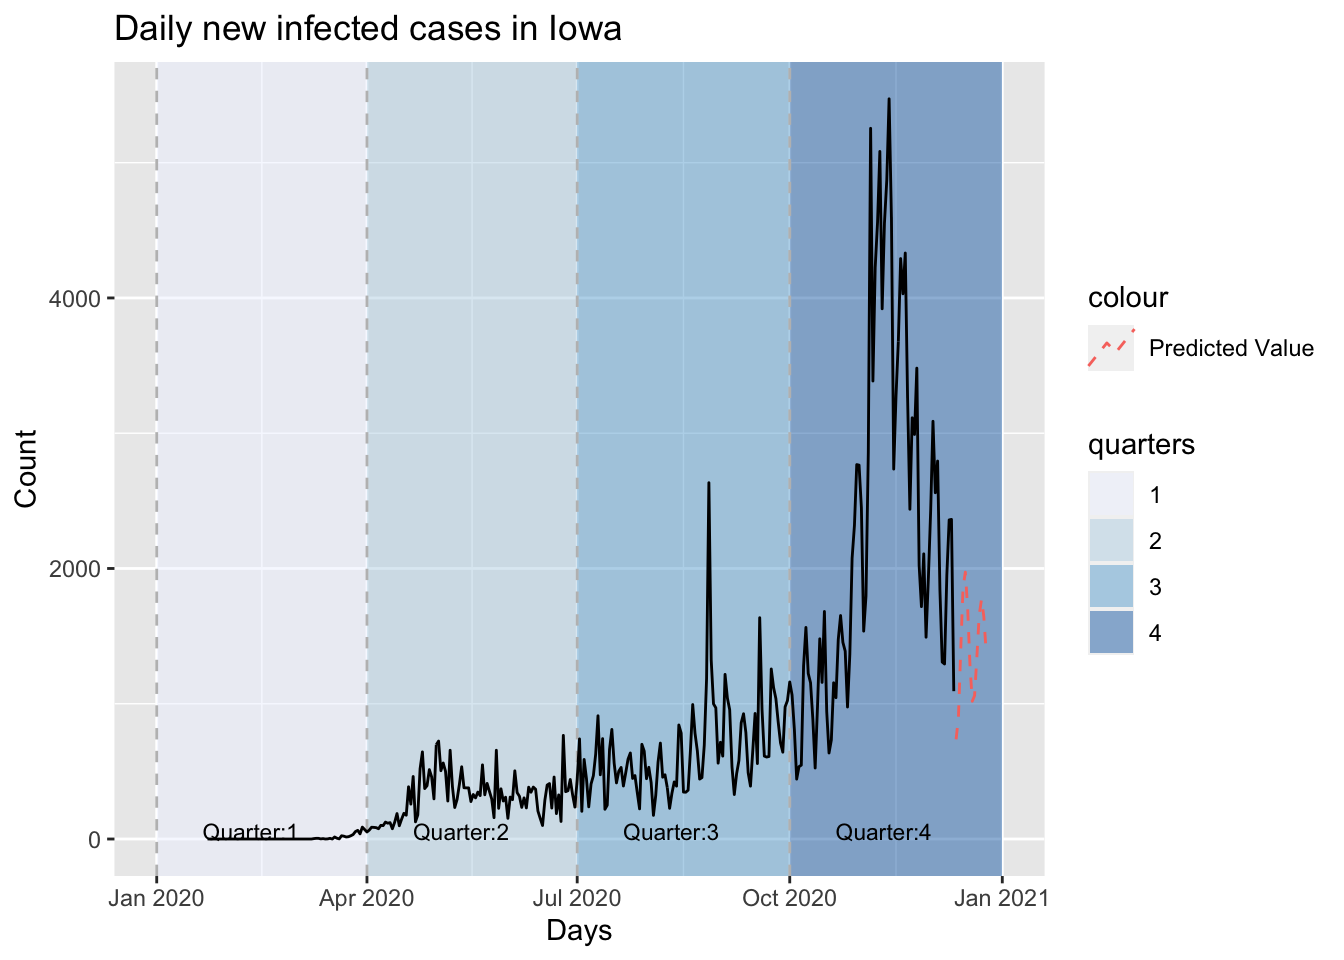
\includegraphics[width=1\linewidth]{bookdown-demo_files/figure-latex/annotate1-1} 

}

\caption{Time series plot with shades and reference lines.}\label{fig:annotate1}
\end{figure}

\section{Maps}\label{maps}

In epidemilogy, data often includes geographical information such as
latitude and longitude or regions like country, state or county. To plot
these types of data, we can extend an existing visualization onto a map
background. We will learn how to make choropleth maps, sometimes called
heat maps, using the \texttt{ggplot2} package. A \textbf{choropleth map}
is a map that shows a geographic landscape with units such as countries,
states, or watersheds where each unit is colored according to a
particular value.

\begin{Shaded}
\begin{Highlighting}[]
\CommentTok{# Read map and data}
\KeywordTok{library}\NormalTok{(ggplot2)}
\KeywordTok{library}\NormalTok{(maps)}
\end{Highlighting}
\end{Shaded}

\begin{verbatim}
## 
## Attaching package: 'maps'
\end{verbatim}

\begin{verbatim}
## The following object is masked from 'package:purrr':
## 
##     map
\end{verbatim}

\begin{Shaded}
\begin{Highlighting}[]
\KeywordTok{library}\NormalTok{(dplyr)}

\CommentTok{# Load United States state map data}
\NormalTok{MainStates <-}\StringTok{ }\KeywordTok{map_data}\NormalTok{(}\StringTok{"state"}\NormalTok{)}
\KeywordTok{head}\NormalTok{(MainStates, }\DecValTok{3}\NormalTok{)}
\end{Highlighting}
\end{Shaded}

\begin{verbatim}
##        long      lat group order  region subregion
## 1 -87.46201 30.38968     1     1 alabama      <NA>
## 2 -87.48493 30.37249     1     2 alabama      <NA>
## 3 -87.52503 30.37249     1     3 alabama      <NA>
\end{verbatim}

\begin{Shaded}
\begin{Highlighting}[]
\NormalTok{MainStates <-}\StringTok{ }\NormalTok{MainStates }\OperatorTok
\StringTok{  }\KeywordTok{mutate}\NormalTok{(}\StringTok{'state'}\NormalTok{ =}\StringTok{ }\KeywordTok{gsub}\NormalTok{(}\StringTok{' '}\NormalTok{, }\StringTok{''}\NormalTok{, MainStates}\OperatorTok{$}\NormalTok{region)) }\OperatorTok
\StringTok{  }\KeywordTok{select}\NormalTok{(}\OperatorTok{-}\KeywordTok{c}\NormalTok{(}\StringTok{'region'}\NormalTok{,}\StringTok{'subregion'}\NormalTok{))}
\KeywordTok{head}\NormalTok{(MainStates, }\DecValTok{3}\NormalTok{)}
\end{Highlighting}
\end{Shaded}

\begin{verbatim}
##        long      lat group order   state
## 1 -87.46201 30.38968     1     1 alabama
## 2 -87.48493 30.37249     1     2 alabama
## 3 -87.52503 30.37249     1     3 alabama
\end{verbatim}

\begin{Shaded}
\begin{Highlighting}[]
\NormalTok{state.long.shape <-}\StringTok{ }\NormalTok{slid}\OperatorTok{::}\NormalTok{state.long }\OperatorTok\StringTok{ }
\StringTok{  }\KeywordTok{mutate}\NormalTok{(}\StringTok{'state'}\NormalTok{ =}\StringTok{ }\KeywordTok{tolower}\NormalTok{(slid}\OperatorTok{::}\NormalTok{state.long}\OperatorTok{$}\NormalTok{State)) }\OperatorTok
\StringTok{  }\KeywordTok{right_join}\NormalTok{(MainStates, }\DataTypeTok{by =} \StringTok{'state'}\NormalTok{) }\OperatorTok
\StringTok{  }\KeywordTok{select}\NormalTok{(}\OperatorTok{-}\NormalTok{state)}
\NormalTok{state.long.shape}
\end{Highlighting}
\end{Shaded}

\begin{verbatim}
## # A tibble: 5,049,525 x 11
##    State Region Division    pop DATE       Infected Death
##    <fct> <fct>  <fct>     <int> <date>        <int> <int>
##  1 Alab~ South  East So~ 4.89e6 2020-12-11   288775  4086
##  2 Alab~ South  East So~ 4.89e6 2020-12-11   288775  4086
##  3 Alab~ South  East So~ 4.89e6 2020-12-11   288775  4086
##  4 Alab~ South  East So~ 4.89e6 2020-12-11   288775  4086
##  5 Alab~ South  East So~ 4.89e6 2020-12-11   288775  4086
##  6 Alab~ South  East So~ 4.89e6 2020-12-11   288775  4086
##  7 Alab~ South  East So~ 4.89e6 2020-12-11   288775  4086
##  8 Alab~ South  East So~ 4.89e6 2020-12-11   288775  4086
##  9 Alab~ South  East So~ 4.89e6 2020-12-11   288775  4086
## 10 Alab~ South  East So~ 4.89e6 2020-12-11   288775  4086
## # ... with 5,049,515 more rows, and 4 more variables:
## #   long <dbl>, lat <dbl>, group <dbl>, order <int>
\end{verbatim}

\begin{Shaded}
\begin{Highlighting}[]
\NormalTok{df <-}\StringTok{ }\NormalTok{state.long.shape }\OperatorTok\StringTok{ }
\StringTok{  }\NormalTok{dplyr}\OperatorTok{::}\KeywordTok{filter}\NormalTok{(DATE }\OperatorTok{==}\StringTok{ '2020-12-11'}\NormalTok{)  }\OperatorTok\StringTok{ }
\StringTok{  }\KeywordTok{mutate}\NormalTok{ (}\DataTypeTok{Risk =}\NormalTok{ Infected }\OperatorTok{/}\StringTok{ }\NormalTok{pop }\OperatorTok{*}\StringTok{ }\DecValTok{1000}\NormalTok{)}
\end{Highlighting}
\end{Shaded}

\subsection{Making a base map}\label{making-a-base-map}

Using \texttt{qplot()}, we can obtain our first map like this:

\begin{Shaded}
\begin{Highlighting}[]
\KeywordTok{qplot}\NormalTok{(long, lat, }\DataTypeTok{geom =} \StringTok{"point"}\NormalTok{, }\DataTypeTok{data =}\NormalTok{ df)}
\end{Highlighting}
\end{Shaded}

\begin{figure}

{\centering 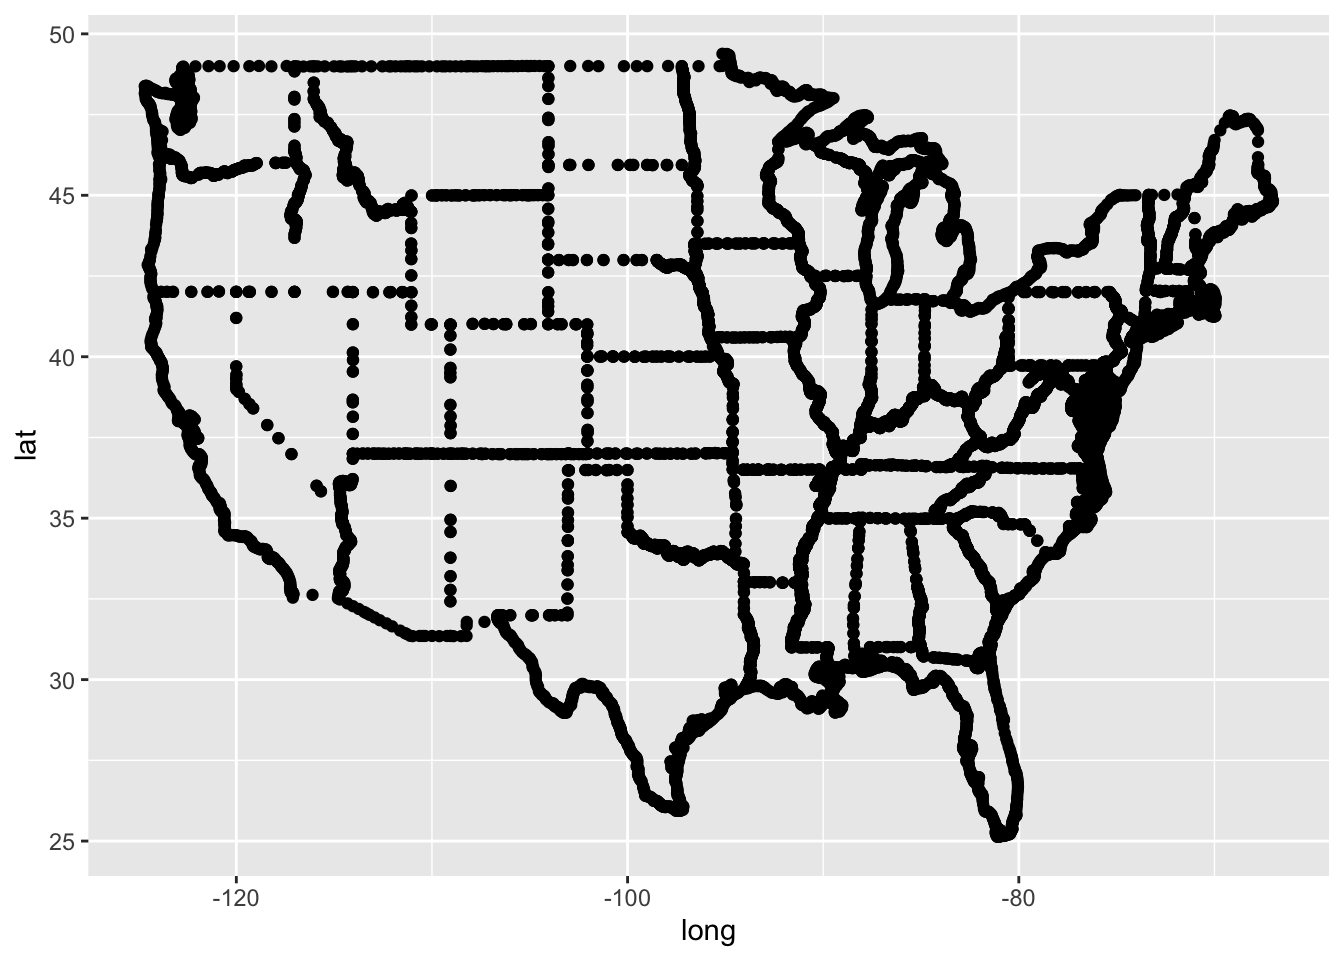
\includegraphics[width=0.75\linewidth]{bookdown-demo_files/figure-latex/unnamed-chunk-59-1} 

}

\caption{Basic US map with dotted state boundaries}\label{fig:unnamed-chunk-59}
\end{figure}

We can use the \texttt{geom\_polygon()} function to create a map with
black borders and add light blue to fill in the map.

\begin{Shaded}
\begin{Highlighting}[]
\CommentTok{# Plot all states with ggplot2, black borders and light blue fill}
\KeywordTok{ggplot}\NormalTok{() }\OperatorTok{+}\StringTok{ }
\StringTok{  }\KeywordTok{geom_polygon}\NormalTok{(}\DataTypeTok{data =}\NormalTok{ df, }
               \KeywordTok{aes}\NormalTok{(}\DataTypeTok{x =}\NormalTok{ long, }\DataTypeTok{y =}\NormalTok{ lat, }\DataTypeTok{group =}\NormalTok{ group),}
                \DataTypeTok{color =} \StringTok{"black"}\NormalTok{, }\DataTypeTok{fill =} \StringTok{"lightblue"}\NormalTok{)}
\end{Highlighting}
\end{Shaded}

\begin{figure}

{\centering 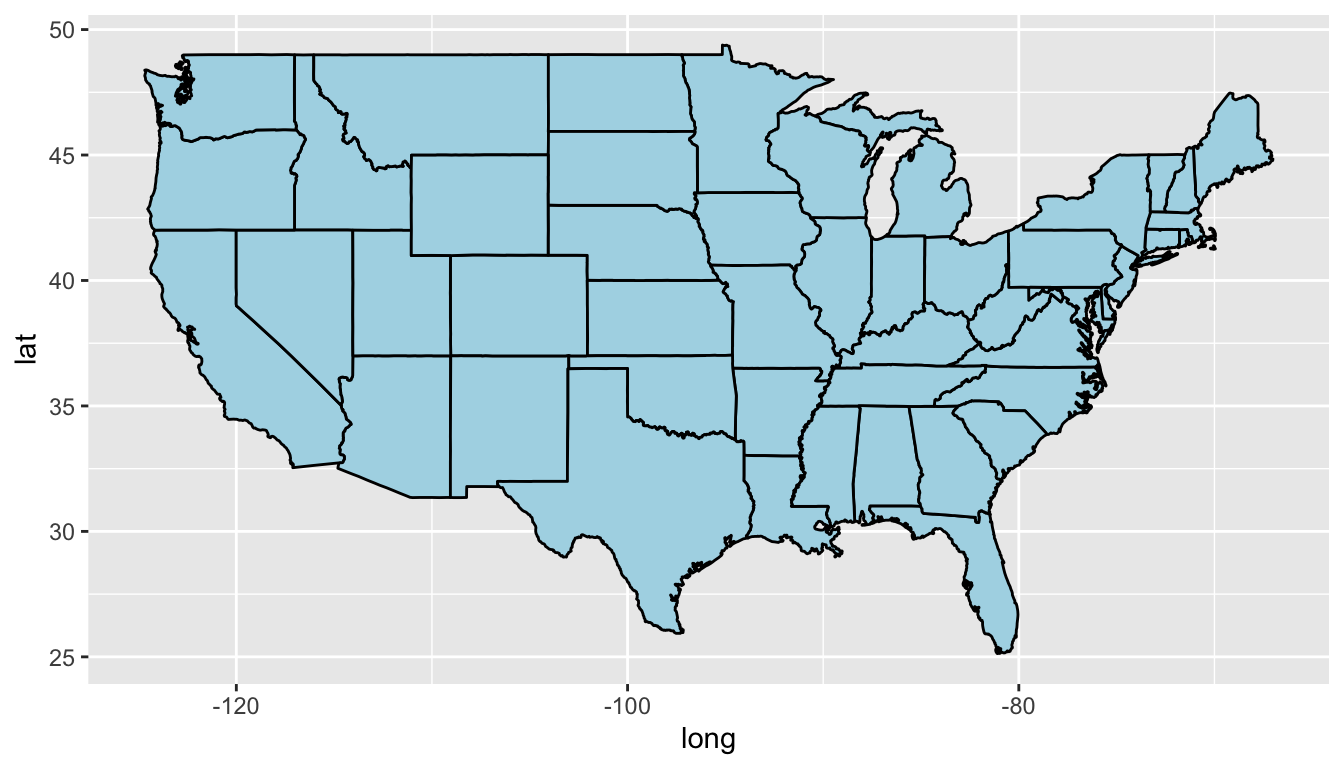
\includegraphics[width=0.75\linewidth]{bookdown-demo_files/figure-latex/unnamed-chunk-60-1} 

}

\caption{US map with colored state areas}\label{fig:unnamed-chunk-60}
\end{figure}

\subsection{\texorpdfstring{Customizing \texttt{choropleth}
map}{Customizing choropleth map}}\label{customizing-choropleth-map}

Now that we have created a base map of the mainland states, we will
color each state according to its the risk. Make the use of
\texttt{slid::ggplot\_map\_state} dataset.

\begin{Shaded}
\begin{Highlighting}[]
\CommentTok{# Create a Choropleth map of the United States}
\NormalTok{p <-}\StringTok{ }\KeywordTok{ggplot}\NormalTok{() }\OperatorTok{+}\StringTok{ }\KeywordTok{geom_polygon}\NormalTok{(}\DataTypeTok{data =}\NormalTok{ df, }
          \KeywordTok{aes}\NormalTok{(}\DataTypeTok{x =}\NormalTok{ long, }\DataTypeTok{y =}\NormalTok{ lat, }\DataTypeTok{group =}\NormalTok{ group, }
              \DataTypeTok{fill =}\NormalTok{ Risk), }
          \DataTypeTok{color =} \StringTok{"white"}\NormalTok{, }\DataTypeTok{size =} \FloatTok{0.2}\NormalTok{) }
\NormalTok{p}
\end{Highlighting}
\end{Shaded}

\begin{figure}

{\centering \includegraphics[width=1\linewidth]{bookdown-demo_files/figure-latex/unnamed-chunk-61-1} 

}

\caption{US map with colored state areas according to infected per thousand population}\label{fig:unnamed-chunk-61}
\end{figure}

\textbf{Remarks}

\begin{itemize}
\item
  Each state is colored by ``Infected per 1000 people'' to make the
  legend easier to read.
\item
  Border color (\texttt{white}) and line thickness
  (\texttt{size\ =\ 0.2}) are specifically defined within this
  \texttt{geom\_polygon()}.
\end{itemize}

Once a map is created, it is often helpful to modify color schemes,
determine how to address missing values (\texttt{na.values}), and
formalize labels. Notice that we assigned the graph a name, \texttt{p}.
This is particularly useful as we add new components to the map.

\begin{Shaded}
\begin{Highlighting}[]
\NormalTok{p }\OperatorTok{+}\StringTok{ }\KeywordTok{scale_fill_continuous}\NormalTok{(}\DataTypeTok{name =} \StringTok{"Infected per 1000 pop"}\NormalTok{,}
                          \DataTypeTok{low =} \StringTok{"yellow"}\NormalTok{, }\DataTypeTok{high =} \StringTok{"darkred"}\NormalTok{,}
                          \DataTypeTok{limits =} \KeywordTok{c}\NormalTok{(}\DecValTok{0}\NormalTok{, }\DecValTok{125}\NormalTok{), }
                          \DataTypeTok{breaks =} \KeywordTok{c}\NormalTok{(}\DecValTok{5}\NormalTok{, }\DecValTok{25}\NormalTok{, }\DecValTok{50}\NormalTok{, }\DecValTok{75}\NormalTok{, }\DecValTok{100}\NormalTok{, }\DecValTok{125}\NormalTok{), }
                          \DataTypeTok{na.value =} \StringTok{"grey50"}\NormalTok{) }\OperatorTok{+}
\StringTok{  }\KeywordTok{labs}\NormalTok{(}\DataTypeTok{title =} \StringTok{"Infected per 1000 population on 2020-12-11"}\NormalTok{)}
\end{Highlighting}
\end{Shaded}

\begin{figure}

{\centering \includegraphics{bookdown-demo_files/figure-latex/unnamed-chunk-62-1} 

}

\caption{US map with colored state areas with limits on the values}\label{fig:unnamed-chunk-62}
\end{figure}

\subsection{Overlay polygon maps}\label{overlay-polygon-maps}

It is also possible to overlay two polygon maps. The code below creates
county borders with a small line size and then adds a thicker line to
represent state borders. The \texttt{alpha\ =\ .3} causes the fill in
the state map to be transparent, allowing us to see the county map
behind the state map.

\begin{Shaded}
\begin{Highlighting}[]
\KeywordTok{ggplot}\NormalTok{() }\OperatorTok{+}\StringTok{ }\KeywordTok{geom_polygon}\NormalTok{(}\DataTypeTok{data =} \KeywordTok{map_data}\NormalTok{(}\StringTok{"county"}\NormalTok{), }
                \KeywordTok{aes}\NormalTok{(}\DataTypeTok{x =}\NormalTok{ long, }\DataTypeTok{y =}\NormalTok{ lat, }\DataTypeTok{group =}\NormalTok{ group),}
                \DataTypeTok{color =} \StringTok{"darkblue"}\NormalTok{, }
                \DataTypeTok{fill =} \StringTok{"lightblue"}\NormalTok{, }\DataTypeTok{size =}\NormalTok{ .}\DecValTok{1}\NormalTok{) }\OperatorTok{+}\StringTok{ }
\StringTok{  }
\StringTok{            }\KeywordTok{geom_polygon}\NormalTok{(}\DataTypeTok{data =} \KeywordTok{map_data}\NormalTok{(}\StringTok{'state'}\NormalTok{), }
                       \KeywordTok{aes}\NormalTok{(}\DataTypeTok{x =}\NormalTok{ long, }\DataTypeTok{y =}\NormalTok{ lat, }\DataTypeTok{group =}\NormalTok{ group),}
                \DataTypeTok{color =} \StringTok{"black"}\NormalTok{, }\DataTypeTok{fill =} \StringTok{"lightblue"}\NormalTok{,  }
                \DataTypeTok{size =}\NormalTok{ .}\DecValTok{5}\NormalTok{, }\DataTypeTok{alpha =}\NormalTok{ .}\DecValTok{3}\NormalTok{) }
\end{Highlighting}
\end{Shaded}

\begin{figure}

{\centering \includegraphics{bookdown-demo_files/figure-latex/unnamed-chunk-63-1} 

}

\caption{US map with colored state areas and county boundaries}\label{fig:unnamed-chunk-63}
\end{figure}

\section{Arranging Plots}\label{arranging-plots}

\subsection{Facet}\label{facet}

Sometimes, we wish to look that the scatterplot within each factor of
categorical variables. For example, we may want to look at the situation
within each \texttt{Region} in our case. We can split a single plot into
many related plots using the function \texttt{facet\_wrap()} or
\texttt{facet\_grid()}:

\begin{itemize}
\item
  \texttt{facet\_wrap(\textasciitilde{}variable)} will return a
  symmetrical matrix of plots for the number of levels of variable;
\item
  \texttt{facet\_grid(.\ \textasciitilde{}variable)} will return facets
  equal to the levels of variable distributed horizontally.
\item
  \texttt{facet\_grid(variable\textasciitilde{}.)} will return facets
  equal to the levels of variable distributed vertically.
\end{itemize}

\begin{Shaded}
\begin{Highlighting}[]
\NormalTok{df <-}\StringTok{ }\NormalTok{slid}\OperatorTok{::}\NormalTok{state.long }\OperatorTok\StringTok{ }
\StringTok{  }\NormalTok{dplyr}\OperatorTok{::}\KeywordTok{filter}\NormalTok{(DATE }\OperatorTok{==}\StringTok{ }\KeywordTok{as.Date}\NormalTok{(}\StringTok{'2020-12-11'}\NormalTok{)) }
\NormalTok{p <-}\StringTok{ }\KeywordTok{ggplot}\NormalTok{(df, }\KeywordTok{aes}\NormalTok{(}\KeywordTok{log}\NormalTok{(Infected }\OperatorTok{+}\StringTok{ }\DecValTok{1}\NormalTok{), }\KeywordTok{log}\NormalTok{(Death }\OperatorTok{+}\StringTok{ }\DecValTok{1}\NormalTok{))) }\OperatorTok{+}\StringTok{ }
\StringTok{  }\KeywordTok{geom_point}\NormalTok{(}\DataTypeTok{na.rm =} \OtherTok{TRUE}\NormalTok{) }\OperatorTok{+}
\StringTok{  }\KeywordTok{aes}\NormalTok{(}\DataTypeTok{color =}\NormalTok{ Region) }

\NormalTok{p}
\end{Highlighting}
\end{Shaded}

\begin{figure}

{\centering \includegraphics[width=0.75\linewidth]{bookdown-demo_files/figure-latex/unnamed-chunk-64-1} 

}

\caption{Facetting examples}\label{fig:unnamed-chunk-64-1}
\end{figure}

\begin{Shaded}
\begin{Highlighting}[]
\NormalTok{p }\OperatorTok{+}\StringTok{ }\KeywordTok{facet_grid}\NormalTok{(.}\OperatorTok{~}\NormalTok{Region)}
\end{Highlighting}
\end{Shaded}

\begin{figure}

{\centering \includegraphics[width=0.75\linewidth]{bookdown-demo_files/figure-latex/unnamed-chunk-64-2} 

}

\caption{Facetting examples}\label{fig:unnamed-chunk-64-2}
\end{figure}

\begin{Shaded}
\begin{Highlighting}[]
\NormalTok{p }\OperatorTok{+}\StringTok{ }\KeywordTok{facet_grid}\NormalTok{(Region}\OperatorTok{~}\NormalTok{.)}
\end{Highlighting}
\end{Shaded}

\begin{figure}

{\centering \includegraphics[width=0.75\linewidth]{bookdown-demo_files/figure-latex/unnamed-chunk-64-3} 

}

\caption{Facetting examples}\label{fig:unnamed-chunk-64-3}
\end{figure}

\begin{Shaded}
\begin{Highlighting}[]
\NormalTok{p }\OperatorTok{+}\StringTok{ }\KeywordTok{facet_wrap}\NormalTok{(}\OperatorTok{~}\NormalTok{Region)}
\end{Highlighting}
\end{Shaded}

\begin{figure}

{\centering \includegraphics[width=0.75\linewidth]{bookdown-demo_files/figure-latex/unnamed-chunk-64-4} 

}

\caption{Facetting examples}\label{fig:unnamed-chunk-64-4}
\end{figure}

\subsection{\texorpdfstring{Combining plots using \texttt{patchwork}
package}{Combining plots using patchwork package}}\label{combining-plots-using-patchwork-package}

Before plots can be laid out, they have to be assembled. The goal of
\texttt{patchwork} is to make it simple to combine separate ggplots into
the same graphic. We can install patchwork from CRAN using

\begin{Shaded}
\begin{Highlighting}[]
\ControlFlowTok{if}\NormalTok{ (}\OperatorTok{!}\KeywordTok{require}\NormalTok{(}\StringTok{'patchwork'}\NormalTok{)) }\KeywordTok{install.packages}\NormalTok{(}\StringTok{'patchwork'}\NormalTok{)}
\KeywordTok{library}\NormalTok{(patchwork)}
\end{Highlighting}
\end{Shaded}

Let us consider some simple examples.

\begin{Shaded}
\begin{Highlighting}[]
\NormalTok{df  <-}\StringTok{ }\NormalTok{slid}\OperatorTok{::}\NormalTok{state.long }\OperatorTok\StringTok{ }
\StringTok{  }\NormalTok{dplyr}\OperatorTok{::}\KeywordTok{filter}\NormalTok{(DATE }\OperatorTok{==}\StringTok{ }\KeywordTok{as.Date}\NormalTok{(}\StringTok{'2020-12-11'}\NormalTok{)) }
\NormalTok{p1 <-}\StringTok{ }\KeywordTok{ggplot}\NormalTok{(df, }\KeywordTok{aes}\NormalTok{(}\KeywordTok{log}\NormalTok{(Infected}\OperatorTok{+}\DecValTok{1}\NormalTok{), }\KeywordTok{log}\NormalTok{(Death }\OperatorTok{+}\StringTok{ }\DecValTok{1}\NormalTok{))) }\OperatorTok{+}\StringTok{ }
\StringTok{  }\KeywordTok{geom_point}\NormalTok{(}\DataTypeTok{na.rm =} \OtherTok{TRUE}\NormalTok{) }

\NormalTok{p2 <-}\StringTok{ }\KeywordTok{ggplot}\NormalTok{(df, }\KeywordTok{aes}\NormalTok{(}\KeywordTok{log}\NormalTok{(Death }\OperatorTok{+}\StringTok{ }\DecValTok{1}\NormalTok{))) }\OperatorTok{+}\StringTok{ }
\StringTok{  }\KeywordTok{geom_histogram}\NormalTok{(}\DataTypeTok{binwidth =} \DecValTok{1}\NormalTok{) }\OperatorTok{+}\StringTok{ }\KeywordTok{aes}\NormalTok{(}\DataTypeTok{fill =}\NormalTok{ Region) }

\NormalTok{p3 <-}\StringTok{ }\KeywordTok{ggplot}\NormalTok{(df, }\KeywordTok{aes}\NormalTok{(}\KeywordTok{log}\NormalTok{(Infected }\OperatorTok{+}\StringTok{ }\DecValTok{1}\NormalTok{))) }\OperatorTok{+}\StringTok{ }
\StringTok{  }\KeywordTok{geom_histogram}\NormalTok{(}\DataTypeTok{binwidth =} \DecValTok{1}\NormalTok{) }\OperatorTok{+}\StringTok{ }\KeywordTok{aes}\NormalTok{(}\DataTypeTok{fill =}\NormalTok{ Region) }

\CommentTok{# Horizontal arrangement}
\NormalTok{p1 }\OperatorTok{+}\StringTok{ }\NormalTok{p2}
\end{Highlighting}
\end{Shaded}

\begin{figure}

{\centering \includegraphics[width=0.75\linewidth]{bookdown-demo_files/figure-latex/unnamed-chunk-66-1} 

}

\caption{Patchwork examples}\label{fig:unnamed-chunk-66-1}
\end{figure}

\begin{Shaded}
\begin{Highlighting}[]
\CommentTok{# Vertical arrangement}
\NormalTok{p1 }\OperatorTok{/}\StringTok{ }\NormalTok{p2}
\end{Highlighting}
\end{Shaded}

\begin{figure}

{\centering \includegraphics[width=0.75\linewidth]{bookdown-demo_files/figure-latex/unnamed-chunk-66-2} 

}

\caption{Patchwork examples}\label{fig:unnamed-chunk-66-2}
\end{figure}

\begin{Shaded}
\begin{Highlighting}[]
\CommentTok{# Grouped arrangements}
\NormalTok{p1 }\OperatorTok{|}\StringTok{ }\NormalTok{(p2 }\OperatorTok{/}\StringTok{ }\NormalTok{p3)}
\end{Highlighting}
\end{Shaded}

\begin{figure}

{\centering \includegraphics[width=0.75\linewidth]{bookdown-demo_files/figure-latex/unnamed-chunk-66-3} 

}

\caption{Patchwork examples}\label{fig:unnamed-chunk-66-3}
\end{figure}

\begin{Shaded}
\begin{Highlighting}[]
\CommentTok{# Combine three plots}
\NormalTok{p1 }\OperatorTok{+}\StringTok{ }\NormalTok{p2 }\OperatorTok{+}\StringTok{ }\NormalTok{p3 }
\end{Highlighting}
\end{Shaded}

\begin{figure}

{\centering \includegraphics[width=0.75\linewidth]{bookdown-demo_files/figure-latex/unnamed-chunk-66-4} 

}

\caption{Patchwork examples}\label{fig:unnamed-chunk-66-4}
\end{figure}

\begin{Shaded}
\begin{Highlighting}[]
\CommentTok{# Set the number of plots per row}
\NormalTok{p1 }\OperatorTok{+}\StringTok{ }\NormalTok{p2 }\OperatorTok{+}\StringTok{ }\NormalTok{p3 }\OperatorTok{+}\StringTok{ }\KeywordTok{plot_layout}\NormalTok{(}\DataTypeTok{ncol =} \DecValTok{2}\NormalTok{)}
\end{Highlighting}
\end{Shaded}

\begin{figure}

{\centering \includegraphics[width=0.75\linewidth]{bookdown-demo_files/figure-latex/unnamed-chunk-66-5} 

}

\caption{Patchwork examples}\label{fig:unnamed-chunk-66-5}
\end{figure}

\begin{Shaded}
\begin{Highlighting}[]
\CommentTok{# Combine the duplicate legends}
\NormalTok{p1 }\OperatorTok{+}\StringTok{ }\NormalTok{p2 }\OperatorTok{+}\StringTok{ }\NormalTok{p3 }\OperatorTok{+}\StringTok{ }\KeywordTok{plot_layout}\NormalTok{(}\DataTypeTok{ncol =} \DecValTok{2}\NormalTok{, }\DataTypeTok{guides =} \StringTok{"collect"}\NormalTok{)}
\end{Highlighting}
\end{Shaded}

\begin{figure}

{\centering \includegraphics[width=0.75\linewidth]{bookdown-demo_files/figure-latex/unnamed-chunk-66-6} 

}

\caption{Patchwork examples}\label{fig:unnamed-chunk-66-6}
\end{figure}

\begin{Shaded}
\begin{Highlighting}[]
\CommentTok{# Add title and subtitles}
\NormalTok{p123 <-}\StringTok{ }\NormalTok{(p1 }\OperatorTok{|}\StringTok{ }\NormalTok{(p2 }\OperatorTok{/}\StringTok{ }\NormalTok{p3))}\OperatorTok{+}\StringTok{ }\KeywordTok{plot_annotation}\NormalTok{(}
  \DataTypeTok{title =} \StringTok{"Add title here"}\NormalTok{,}
  \DataTypeTok{caption =} \StringTok{"Add caption here"}
\NormalTok{)}
\NormalTok{p123}
\end{Highlighting}
\end{Shaded}

\begin{figure}

{\centering \includegraphics[width=0.75\linewidth]{bookdown-demo_files/figure-latex/unnamed-chunk-66-7} 

}

\caption{Patchwork examples}\label{fig:unnamed-chunk-66-7}
\end{figure}

\section{Output}\label{output}

After polishing the figure, we need to save the figure and output it as
a readable file for later use. We can either output it in a standard
figure format, such as png, tiff, jpeg; or we can save it as an R
readable data file, usually referred to as \texttt{XXX.rds},
\texttt{XXX.rda} or \texttt{XXX.RData}, and read by
\texttt{readRDS(\textquotesingle{}XXX.rds\textquotesingle{})}.

\subsection{Save in figure format}\label{save-in-figure-format}

\begin{Shaded}
\begin{Highlighting}[]
\CommentTok{# Take a look at the figure before saving}
\CommentTok{# print(p) }
\KeywordTok{ggsave}\NormalTok{(}\StringTok{'example_ggplot2.png'}\NormalTok{, p) }\CommentTok{# Save the figure in png format}
\end{Highlighting}
\end{Shaded}

\begin{verbatim}
## Saving 6.5 x 4.5 in image
\end{verbatim}

\subsection{Save in RDS format}\label{save-in-rds-format}

\begin{Shaded}
\begin{Highlighting}[]
\CommentTok{# Save the figure in .rda format}
\KeywordTok{saveRDS}\NormalTok{(p, }\StringTok{'example_ggplot2.rds'}\NormalTok{) }
\CommentTok{# Read the figure in .rda format}
\NormalTok{q <-}\StringTok{ }\KeywordTok{readRDS}\NormalTok{(}\StringTok{'example_ggplot2.rds'}\NormalTok{)}
\CommentTok{# print(q)}
\end{Highlighting}
\end{Shaded}

\section{Exercises}\label{exercises-1}

\begin{enumerate}
\def\labelenumi{\arabic{enumi}.}
\tightlist
\item
  Scatter plot using \texttt{slid::state.long} on 2020-11-01.
\end{enumerate}

\begin{enumerate}
\def\labelenumi{\alph{enumi}.}
\tightlist
\item
  Create a scatter plot. Treat \texttt{Infected/1000} as x-axis, and
  \texttt{Death/1000} as y-axis.
\item
  Color the points according to \texttt{Division}. Hint: use
  \texttt{aes(color\ =\ )}.
\item
  Change the size of the points to be proportional to population. Hint:
  use \texttt{aes(size\ =\ )}.
\item
  Change the label of x-axis to `Infected (in thousands)', the label of
  y-axis to `Death(in thousands)'.
\item
  Change the title of the figure as `Infected against death on
  2020-11-01'.
\item
  Save the plot to file `q1.png'.
\end{enumerate}

\begin{enumerate}
\def\labelenumi{\arabic{enumi}.}
\setcounter{enumi}{1}
\tightlist
\item
  Time series plot using \texttt{slid::state.ts} for Florida.
\end{enumerate}

\begin{enumerate}
\def\labelenumi{\alph{enumi}.}
\tightlist
\item
  Obtain the daily new death count for Florida.
\item
  Create a line plot, time as x-axis, daily new death as y-axis. Add the
  title ``Daily new death count for Florida'' to the plot.
\item
  Using the data up till 2020-11-27, a model obtained the following
  prediction and 80\% prediction intervals for the period from
  2020-11-28 to 2020-12-11.
\end{enumerate}

\begin{verbatim}
    DATE   Y.Death    PI
1 2020-11-28   72  [33, 111]
2 2020-11-29   56  [17,  96]
3 2020-11-30   74  [34, 114]
4 2020-12-01   88  [48, 128]
5 2020-12-02   91  [50, 131]
6 2020-12-03   59  [18, 101]
7 2020-12-04  104  [62, 146]
8 2020-12-05   79  [31, 128]
9 2020-12-06   64  [14, 113]
10 2020-12-07  81  [31, 132]
11 2020-12-08  95  [43, 148]
12 2020-12-09  98  [44, 152]
13 2020-12-10  67  [12, 122]
14 2020-12-11 111  [54, 168]
\end{verbatim}

Add another line on your time series plot indicating the predicted daily
new death data. Change the title to ``Two weeks ahead forecast of the
daily new death count for Florida'' your plot.

\begin{enumerate}
\def\labelenumi{\alph{enumi}.}
\setcounter{enumi}{3}
\item
  Add ribbons on your time series plot in part c to illustrate the
  prediction intervals in part c. Change the title to ``Two weeks ahead
  forecast of the daily new death count for Florida with 80\% prediction
  intervals''.
\item
  Save the plot to file `q2.png'.
\end{enumerate}

\begin{enumerate}
\def\labelenumi{\arabic{enumi}.}
\setcounter{enumi}{2}
\tightlist
\item
  For the data \texttt{slid::state.long} and focus on 2020-11-01, do the
  following:
\end{enumerate}

\begin{enumerate}
\def\labelenumi{\alph{enumi}.}
\tightlist
\item
  Create a map using Death per 1000 population as the coloring feature.
\item
  Save the plot to file `q3.png'.
\end{enumerate}

\begin{enumerate}
\def\labelenumi{\arabic{enumi}.}
\setcounter{enumi}{3}
\tightlist
\item
  Combine the three figures and save the plot to file `q4.png'. Hint: In
  \texttt{R}, save each plot with different names (e.g. \texttt{p1},
  \texttt{p2}, \texttt{p3}), and then use the \texttt{patchwork}
  package.
\end{enumerate}

\chapter{Interactive Visualization}\label{plotly}

\section{An Introduction}\label{an-introduction}

As the volume and complexity of infectious disease data increases,
public health professionals must synthesize highly disparate data to
facilitate communication with the public and inform decisions regarding
measures to protect the public's health. Interactive data visualization
allows users the freedom to explore data fully. Here are some key
advantages of using interactive data visualization software:

\begin{itemize}
\tightlist
\item
  Hovering over any data point to see the data behind it;
\item
  Identifying causes and trends more quickly;
\item
  Adding multiple highlights and change view subsets of the data by
  editing options below each graph;
\item
  Auto-refreshing your visuals to show the most recent data.
\end{itemize}

So far, your primary tool for creating these data visualizations has
been ``ggplots''. In the past few years, interactive tools for
visualization of disease outbreaks has been improving markedly. In this
chapter, we will introduce the R \texttt{plotly} package, which allows
you to make more professional and interactive graphics, share them on
websites, and customize them as you wish.

\begin{figure}

{\centering \includegraphics[width=0.8\linewidth]{figures/process3} 

}

\caption{A typical data science process.}\label{fig:process3}
\end{figure}

Plotly is an R package for creating interactive, publication-quality
graphs. Some of the charts you can do are Basic charts, Statistical
charts, Scientific charts, Financial charts, Maps, 3D charts, Subplots,
Transforms, Animations. Plotly is built on top of visualization library
D3.js, HTML, and CSS. Here are some benefits of using plotly.

\begin{itemize}
\tightlist
\item
  Plotly is compatible with several languages/ tools: R, Python, MATLAB,
  Perl, Julia, Arduino.
\item
  Using plotly, we can easily share interactive plots online with
  multiple people.
\item
  Plotly can also be used by people with no technical background for
  creating interactive plots by uploading the data and using plotly GUI.
\item
  Plotly is compatible with ggplots in R and Python.
\item
  Plotly allows embedding interactive plots in websites using iframes or
  HTML.
\item
  The syntax for creating interactive plots using plotly is
  straightforward as well.
\end{itemize}

\textbf{Suggested references:}

\begin{itemize}
\tightlist
\item
  \url{https://plotly-r.com/overview.html}
\item
  \url{https://plot.ly/r}
\item
  \url{https://plot.ly/r/reference/}
\item
  Read the book \citet{Sievert2020}:
  \href{https://plotly-r.com}{Interactive web-based data visualization
  with R, plotly, and shiny}.
\item
  Read the
  \href{https://images.plot.ly/plotly-documentation/images/plotly_js_cheat_sheet.pdf?_ga=2.148726517.312656595.1565006727-1010438718.1562929967}{Cheatsheet}
  from \url{https://images.plot.ly/}.
\end{itemize}

Before we begin, please get ready by installing the \texttt{plotly} R
package by any of the following methods.

\textbf{Install \texttt{Plotly}}

You can download the package by using written code below:

\begin{Shaded}
\begin{Highlighting}[]
\KeywordTok{install.packages}\NormalTok{(}\StringTok{"plotly"}\NormalTok{)}
\end{Highlighting}
\end{Shaded}

\textbf{Install from Github}

Alternatively, you can install the latest development version of plotly
from GitHub via the \texttt{devtools} R package:

\begin{Shaded}
\begin{Highlighting}[]
\NormalTok{devtools}\OperatorTok{::}\KeywordTok{install_github}\NormalTok{(}\StringTok{"ropensci/plotly"}\NormalTok{)}
\end{Highlighting}
\end{Shaded}

\section{Creating Plotly Objects}\label{creating-plotly-objects}

To create a plotly object, you start with a call to \texttt{plotly()}
and pass the data. Next, you decide which graphical representation you
want to use: points, lines, bar charts, etc. Then, you customize labels,
colors, titles, fonts, etc. Here is a typical code structure:

\begin{Shaded}
\begin{Highlighting}[]
\KeywordTok{plot_ly}\NormalTok{(data) }\OperatorTok\StringTok{ }
\NormalTok{add_}\OperatorTok{*}\StringTok{ }\NormalTok{(x, y, type, mode, color, size) }\OperatorTok\StringTok{ }
\KeywordTok{layout}\NormalTok{(title, }\DataTypeTok{xaxis =} \KeywordTok{list}\NormalTok{(title, titlefont), }
       \DataTypeTok{yaxis =} \KeywordTok{list}\NormalTok{(title, titlefont))}
\end{Highlighting}
\end{Shaded}

In the above code, \texttt{layout()} is used to add/modify part(s) of
the graph's layout. There are a family of \texttt{add\_*()} functions,
such as \texttt{add\_histogram()}, \texttt{add\_trace()},
\texttt{add\_lines()}, \texttt{add\_pie()}, that you can define how to
render data into geometric objects. These functions add a graphical
layer to a plot. A layer can be considered as a group of graphical
elements that can be sufficiently described using only five components:

\begin{itemize}
\tightlist
\item
  data,
\item
  aesthetic mappings (e.g., assigning clarity to color),
\item
  a geometric representation (e.g., rectangles, circles, etc.),
\item
  statistical transformations (e.g., sum, mean, etc.),
\item
  and positional adjustments (e.g., dodge, stack, etc.).
\end{itemize}

Here are some arguments that are typically used in the \texttt{add\_*()}
function:

\begin{itemize}
\tightlist
\item
  \texttt{x}: values for x-axis;
\item
  \texttt{y}: values for y-axis;
\item
  \texttt{type}: to specify the plot that you want to create like
  ``histogram'', ``bar'', ``scatter'', etc.
\item
  \texttt{mode}: format in which you want data to be represented in the
  plot, and possible values are ``markers'', ``lines, ``points'';
\item
  \texttt{color}: values of same length as \texttt{x}, \texttt{y} and
  \texttt{z} that represents the color of data points or lines in plot.
\item
  \texttt{size}: values for same length as \texttt{x}, \texttt{y} and
  \texttt{z} that represents the size of data points or lines in plot.
\end{itemize}

\subsection{\texorpdfstring{Using \texttt{plot\_ly()} to create a plotly
object}{Using plot\_ly() to create a plotly object}}\label{using-plot_ly-to-create-a-plotly-object}

Before you try this example, please make sure to install
\texttt{plotly}, \texttt{dplyr} and \texttt{lubridate} packages. The
\texttt{lubridate} is an R package of choice for working with variables
that store dates' values.

\begin{Shaded}
\begin{Highlighting}[]
\KeywordTok{library}\NormalTok{(lubridate)}
\KeywordTok{library}\NormalTok{(dplyr)}
\KeywordTok{library}\NormalTok{(plotly)}
\end{Highlighting}
\end{Shaded}

The county-level dataset is used to create the bar chart below. You can
download the \texttt{county.top10} dataset from the \texttt{slid} R
package. This data contains the top 10 counties with the largest number
of infected cases on 2020/12/11.

\begin{Shaded}
\begin{Highlighting}[]
\KeywordTok{library}\NormalTok{(devtools)}
\KeywordTok{install_github}\NormalTok{(}\StringTok{'covid19-dashboard-us/slid'}\NormalTok{)}
\end{Highlighting}
\end{Shaded}

\begin{Shaded}
\begin{Highlighting}[]
\KeywordTok{library}\NormalTok{(slid)}
\KeywordTok{data}\NormalTok{(county.top10)}
\NormalTok{county.top10}
\end{Highlighting}
\end{Shaded}

\begin{verbatim}
##         ID        County      State Infection Death
## 176   6037    LosAngeles California    501635  8199
## 577  17031          Cook   Illinois    346004  7282
## 334  12086    Miami-Dade    Florida    253403  3959
## 75    4013      Maricopa    Arizona    245671  4299
## 2586 48201        Harris      Texas    204850  3128
## 2542 48113        Dallas      Texas    156225  1751
## 1715 32003         Clark     Nevada    137100  1962
## 193   6071 SanBernardino California    120186  1209
## 297  12011       Broward    Florida    118512  1728
## 2705 48439       Tarrant      Texas    116931  1158
\end{verbatim}

Now let's use the \texttt{plot\_ly()} to initialize a plotly object.

\begin{Shaded}
\begin{Highlighting}[]
\KeywordTok{plot_ly}\NormalTok{(}\DataTypeTok{data =}\NormalTok{ county.top10) }\OperatorTok\StringTok{ }
\StringTok{  }\KeywordTok{add_trace}\NormalTok{(}\DataTypeTok{y =} \OperatorTok{~}\NormalTok{Infection, }\DataTypeTok{x =} \OperatorTok{~}\NormalTok{County, }\DataTypeTok{type =} \StringTok{'bar'}\NormalTok{, }
            \DataTypeTok{name =} \StringTok{'Infection'}\NormalTok{)}
\end{Highlighting}
\end{Shaded}

\begin{figure}

{\centering \includegraphics{bookdown-demo_files/figure-latex/bar0-1} 

}

\caption{Bar chart of the infected count.}\label{fig:bar0}
\end{figure}

Here are a few things that you can try in the interactive plots:

\begin{itemize}
\tightlist
\item
  Hovering your mouse over the plot to view associated attributes;
\item
  Selecting a particular region on the plot using your mouse to zoom;
\item
  Resetting the axis;
\item
  Zooming in and zooming out.
\end{itemize}

Next, you can use \texttt{layout()} to modify the layout of a plotly
visualization and specify more complex plot arrangements.

\begin{Shaded}
\begin{Highlighting}[]
\KeywordTok{plot_ly}\NormalTok{(}\DataTypeTok{data =}\NormalTok{ county.top10) }\OperatorTok\StringTok{ }
\StringTok{  }\KeywordTok{add_trace}\NormalTok{(}\DataTypeTok{y =} \OperatorTok{~}\NormalTok{Infection, }\DataTypeTok{x =} \OperatorTok{~}\NormalTok{County, }\DataTypeTok{type =} \StringTok{'bar'}\NormalTok{, }
            \DataTypeTok{name =} \StringTok{'Infection'}\NormalTok{) }\OperatorTok
\StringTok{  }\KeywordTok{layout}\NormalTok{(}\DataTypeTok{xaxis =} \KeywordTok{list}\NormalTok{(}\DataTypeTok{title =} \StringTok{"County"}\NormalTok{), }
         \DataTypeTok{yaxis =} \KeywordTok{list}\NormalTok{(}\DataTypeTok{title =}\StringTok{"Infected Count"}\NormalTok{),}
         \DataTypeTok{title =} \StringTok{"Total Infected Cases on 2020-12-11"}\NormalTok{)}
\end{Highlighting}
\end{Shaded}

\begin{figure}

{\centering \includegraphics{bookdown-demo_files/figure-latex/bar1-1} 

}

\caption{Modified bargraph of the infected count.}\label{fig:bar1}
\end{figure}

You can also add text labels and annotations to a plotly project in R
using \texttt{add\_text()}.

\begin{Shaded}
\begin{Highlighting}[]
\KeywordTok{plot_ly}\NormalTok{(}\DataTypeTok{data =}\NormalTok{ county.top10) }\OperatorTok\StringTok{ }
\StringTok{  }\KeywordTok{add_bars}\NormalTok{(}\DataTypeTok{y =} \OperatorTok{~}\NormalTok{Infection, }\DataTypeTok{x =} \OperatorTok{~}\NormalTok{County, }\DataTypeTok{name =} \StringTok{'Infection'}\NormalTok{) }\OperatorTok\StringTok{ }
\StringTok{  }\KeywordTok{add_text}\NormalTok{(}
    \DataTypeTok{text =} \OperatorTok{~}\NormalTok{scales}\OperatorTok{::}\KeywordTok{comma}\NormalTok{(Infection), }\DataTypeTok{y =} \OperatorTok{~}\NormalTok{Infection, }\DataTypeTok{x =} \OperatorTok{~}\NormalTok{County,}
    \DataTypeTok{textposition =} \StringTok{"top middle"}\NormalTok{, }\DataTypeTok{showlegend =} \OtherTok{FALSE}\NormalTok{,}
    \DataTypeTok{cliponaxis =} \OtherTok{FALSE}
\NormalTok{  ) }\OperatorTok
\StringTok{  }\KeywordTok{add_bars}\NormalTok{(}\DataTypeTok{y =} \OperatorTok{~}\NormalTok{Death, }\DataTypeTok{x =} \OperatorTok{~}\NormalTok{County, }\DataTypeTok{name =} \StringTok{'Death'}\NormalTok{, }
           \DataTypeTok{color =} \KeywordTok{I}\NormalTok{(}\StringTok{"red"}\NormalTok{)) }\OperatorTok\StringTok{ }
\StringTok{    }\KeywordTok{add_text}\NormalTok{(}
    \DataTypeTok{text =} \OperatorTok{~}\NormalTok{Death, }\DataTypeTok{y =} \OperatorTok{~}\NormalTok{Death, }\DataTypeTok{x =} \OperatorTok{~}\NormalTok{County,}
    \DataTypeTok{textposition =} \StringTok{"top middle"}\NormalTok{,  }\DataTypeTok{showlegend =} \OtherTok{FALSE}\NormalTok{,}
    \DataTypeTok{cliponaxis =} \OtherTok{FALSE}
\NormalTok{  ) }\OperatorTok
\StringTok{  }\KeywordTok{layout}\NormalTok{(}\DataTypeTok{xaxis =} \KeywordTok{list}\NormalTok{(}\DataTypeTok{title =} \StringTok{"County"}\NormalTok{), }
         \DataTypeTok{yaxis =} \KeywordTok{list}\NormalTok{(}\DataTypeTok{title =} \StringTok{"Number of Cases"}\NormalTok{),}
         \DataTypeTok{title =} \StringTok{"Total Infected/Death Cases on 2020-12-11"}\NormalTok{)}
\end{Highlighting}
\end{Shaded}

\begin{figure}

{\centering \includegraphics{bookdown-demo_files/figure-latex/bar2-1} 

}

\caption{Bargraph of the infected count and death count.}\label{fig:bar2}
\end{figure}

\subsection{\texorpdfstring{Use \texttt{dplyr} verbs to modify
data}{Use dplyr verbs to modify data}}\label{use-dplyr-verbs-to-modify-data}

To visualize the states that the counties with the most infected cases
locate in, we can use the \texttt{dplyr} verbs to modify data and
calculate counts and use \texttt{add\_bars} to add a new bar chart.

\begin{Shaded}
\begin{Highlighting}[]
\NormalTok{county.top10 }\OperatorTok
\StringTok{  }\KeywordTok{group_by}\NormalTok{(State) }\OperatorTok
\StringTok{  }\KeywordTok{summarise}\NormalTok{(}\DataTypeTok{n =} \KeywordTok{n}\NormalTok{()) }\OperatorTok
\StringTok{  }\KeywordTok{plot_ly}\NormalTok{() }\OperatorTok\StringTok{ }
\StringTok{  }\KeywordTok{add_bars}\NormalTok{(}\DataTypeTok{x =} \OperatorTok{~}\NormalTok{State, }\DataTypeTok{y =} \OperatorTok{~}\NormalTok{n)}
\end{Highlighting}
\end{Shaded}

\begin{figure}

{\centering \includegraphics{bookdown-demo_files/figure-latex/bar4-1} 

}

\caption{Bargraph of the infected count by adding bars.}\label{fig:bar4}
\end{figure}

Next, suppose we are interested in the distribution of the logarithm of
the daily new infected cases from 2020-11-12 to 2020-12-11 from all the
states in the US. We can use the \texttt{state.long} data in the
\texttt{slid} R package, and plot the histogram of log(daily new
infected cases) using \texttt{add\_histogram}.

\begin{Shaded}
\begin{Highlighting}[]
\CommentTok{# Prepare the daily new Infected for each state in the period }
\CommentTok{# from 2020-11-12 to 2020-12-11}
\NormalTok{slid}\OperatorTok{::}\NormalTok{state.long }\OperatorTok
\NormalTok{dplyr}\OperatorTok{::}\KeywordTok{filter}\NormalTok{(DATE }\OperatorTok{<=}\StringTok{ '2020-12-11'} \OperatorTok{&}\StringTok{ }\NormalTok{DATE }\OperatorTok{>}\StringTok{ '2020-11-11'}\NormalTok{) }\OperatorTok
\KeywordTok{group_by}\NormalTok{(State) }\OperatorTok\StringTok{ }\CommentTok{# Group by State}
\CommentTok{# Create daily new from cum. Infected count}
\KeywordTok{mutate}\NormalTok{(}\DataTypeTok{Y.Infected =} \KeywordTok{c}\NormalTok{(Infected[}\OperatorTok{-}\KeywordTok{length}\NormalTok{(Infected)] }\OperatorTok{-}\StringTok{ }\NormalTok{Infected[}\OperatorTok{-}\DecValTok{1}\NormalTok{], }\DecValTok{0}\NormalTok{)) }\OperatorTok\StringTok{ }
\StringTok{  }\KeywordTok{plot_ly}\NormalTok{() }\OperatorTok
\StringTok{  }\KeywordTok{add_histogram}\NormalTok{(}\DataTypeTok{x =} \OperatorTok{~}\KeywordTok{log}\NormalTok{(Y.Infected}\OperatorTok{+}\DecValTok{1}\NormalTok{))}
\end{Highlighting}
\end{Shaded}

\begin{figure}

{\centering \includegraphics{bookdown-demo_files/figure-latex/bar3-1} 

}

\caption{Histogram of the log(daily new infected cases).}\label{fig:bar3}
\end{figure}

\subsection{\texorpdfstring{Using \texttt{ggplotly()} to create a
\texttt{plotly}
object}{Using ggplotly() to create a plotly object}}\label{using-ggplotly-to-create-a-plotly-object}

The \texttt{ggplotly()} function from the \texttt{plotly} package has
the ability to translate \texttt{ggplot2} to plotly. This functionality
can be really helpful for quickly adding interactivity to your existing
ggplot2 workflow.

We consider the \texttt{state.long} dataset, which includes the
variables, cumulative infected cases (\texttt{Infected}). Chapter
\ref{ggplot2} shows how to draw a simple scatterplot using the reported
data on December 11, 2020. Figure \ref{fig:ggplotly1} shows a translated
scatterplot from \texttt{ggplot2} to \texttt{plotly}.

\begin{Shaded}
\begin{Highlighting}[]
\NormalTok{df <-}\StringTok{ }\NormalTok{slid}\OperatorTok{::}\NormalTok{state.long }\OperatorTok\StringTok{ }\NormalTok{dplyr}\OperatorTok{::}\KeywordTok{filter}\NormalTok{(DATE }\OperatorTok{==}\StringTok{ '2020-12-11'}\NormalTok{) }

\NormalTok{p <-}\StringTok{ }\KeywordTok{ggplot}\NormalTok{(df, }\KeywordTok{aes}\NormalTok{(}\KeywordTok{log}\NormalTok{(Infected), }\KeywordTok{log}\NormalTok{(Death))) }\OperatorTok{+}\StringTok{              }
\StringTok{            }\KeywordTok{geom_point}\NormalTok{() }\OperatorTok{+}\StringTok{ }
\StringTok{  }\KeywordTok{geom_point}\NormalTok{(}\KeywordTok{aes}\NormalTok{(}\DataTypeTok{color =}\NormalTok{ Region)) }
\CommentTok{# Translate ggplot2 to plotly}
\KeywordTok{ggplotly}\NormalTok{(p)}
\end{Highlighting}
\end{Shaded}

\begin{figure}

{\centering \includegraphics[width=1\linewidth]{bookdown-demo_files/figure-latex/ggplotly1-1} 

}

\caption{A translated scatterplot from ggplot2 to to plotly.}\label{fig:ggplotly1}
\end{figure}

\section{Scatterplots and Line Plots}\label{scatterplots-and-line-plots}

The \texttt{plot\_ly()} function initiates an object where one or
multiple traces can be added to it via functions \texttt{add\_trace()}
or \texttt{add\_*()}. In \texttt{add\_trace()}, the layer's type can be
specified using the \texttt{type} argument. For example, some most
commonly used types include
\texttt{\textquotesingle{}scatter\textquotesingle{}},
\texttt{\textquotesingle{}bar\textquotesingle{}},
\texttt{\textquotesingle{}box\textquotesingle{}},
\texttt{\textquotesingle{}histogram\textquotesingle{}},
\texttt{\textquotesingle{}heatmap\textquotesingle{}}, etc. Some
\texttt{add\_*()} functions are specific cases of a trace type. If the
type is not specified when adding a layer, a sensible default will be
set.

We focus on
\texttt{type\ =\ \textquotesingle{}scatter\textquotesingle{}}, which
works well in displaying lines and points, such as the time series of
infected cases or the number of people vaccinated during the pandemic.

\subsection{Make a scatterplot}\label{make-a-scatterplot}

We use the \texttt{state.long} data to draw a basic scatterplot with
log(Death) vs log(Infected).

\begin{Shaded}
\begin{Highlighting}[]
\KeywordTok{library}\NormalTok{(slid)}
\KeywordTok{data}\NormalTok{(state.long)}

\KeywordTok{plot_ly}\NormalTok{(}\DataTypeTok{data =}\NormalTok{ state.long }\OperatorTok\StringTok{ }
\StringTok{          }\KeywordTok{filter}\NormalTok{(DATE }\OperatorTok{==}\StringTok{ }\KeywordTok{as.Date}\NormalTok{(}\StringTok{'2020-12-11'}\NormalTok{))) }\OperatorTok\StringTok{ }
\StringTok{  }\KeywordTok{add_trace}\NormalTok{(}\DataTypeTok{x =} \OperatorTok{~}\KeywordTok{log}\NormalTok{(Infected), }\DataTypeTok{y =} \OperatorTok{~}\KeywordTok{log}\NormalTok{(Death), }\DataTypeTok{text =} \OperatorTok{~}\NormalTok{State, }
            \DataTypeTok{type =} \StringTok{'scatter'}\NormalTok{, }\DataTypeTok{mode =} \StringTok{'markers'}\NormalTok{)}
\end{Highlighting}
\end{Shaded}

\includegraphics{bookdown-demo_files/figure-latex/unnamed-chunk-75-1.pdf}

\subsection{Markers}\label{markers}

We now describe how to change the point colors, and shapes of markers
generated using plotly.

\begin{itemize}
\item
  \texttt{color}: values mapped to relevant fill-color' attribute(s);

  \begin{itemize}
  \tightlist
  \item
    \texttt{I()}: avoid mapping a data value to colors and specify the
    color manually (e.g., \texttt{color\ =\ I("red")}).
  \item
    variable:

    \begin{itemize}
    \tightlist
    \item
      numeric: generate one trace with a filled color determined by the
      variable value and a color bar as a guide;
    \item
      factor: generate multiple traces with different colors, one for
      each factor level;
    \end{itemize}
  \end{itemize}
\item
  \texttt{symbol}: can be specified similarly as \texttt{color}

  \begin{itemize}
  \tightlist
  \item
    by factor value;
  \item
    \texttt{I()} to set a fixed color.
  \end{itemize}
\item
  \texttt{size}: for scatterplots, unless otherwise specified via the
  \texttt{sizemode}, the size argument controls the area of markers and
  must be a numeric variable. The \texttt{size} argument controls the
  minimum and maximum size of circles in pixels.
\end{itemize}

Below, we customize the scatterplot and change the size and color of the
markers.

\begin{Shaded}
\begin{Highlighting}[]
\KeywordTok{data}\NormalTok{(state.long)}
\KeywordTok{plot_ly}\NormalTok{(}\DataTypeTok{data =}\NormalTok{ state.long }\OperatorTok\StringTok{ }
\StringTok{          }\KeywordTok{filter}\NormalTok{(DATE }\OperatorTok{==}\StringTok{ }\KeywordTok{as.Date}\NormalTok{(}\StringTok{'2020-12-11'}\NormalTok{))) }\OperatorTok\StringTok{ }
\StringTok{  }\KeywordTok{add_trace}\NormalTok{(}\DataTypeTok{x =} \OperatorTok{~}\KeywordTok{log}\NormalTok{(Infected), }\DataTypeTok{y =} \OperatorTok{~}\KeywordTok{log}\NormalTok{(Death), }\DataTypeTok{text =} \OperatorTok{~}\NormalTok{State, }
            \DataTypeTok{type =} \StringTok{'scatter'}\NormalTok{, }\DataTypeTok{mode =} \StringTok{'markers'}\NormalTok{, }
            \CommentTok{# change the size and color of the markers}
            \DataTypeTok{size =} \OperatorTok{~}\NormalTok{pop, }\DataTypeTok{color =} \OperatorTok{~}\NormalTok{Region, }
            \DataTypeTok{marker =} \KeywordTok{list}\NormalTok{(}\DataTypeTok{opacity =} \FloatTok{0.5}\NormalTok{, }\DataTypeTok{symbol =} \StringTok{'circle'}\NormalTok{, }
                          \DataTypeTok{sizemode =} \StringTok{'diameter'}\NormalTok{)) }
\end{Highlighting}
\end{Shaded}

\includegraphics{bookdown-demo_files/figure-latex/unnamed-chunk-76-1.pdf}

\subsection{A single time series plot}\label{a-single-time-series-plot}

We draw a time series of the cumulative infected count for Cook county,
IL.

\begin{Shaded}
\begin{Highlighting}[]
\CommentTok{# Load data}
\KeywordTok{library}\NormalTok{(slid)}
\KeywordTok{data}\NormalTok{(county.top10.long)}

\CommentTok{# Start plotly from here}
\KeywordTok{plot_ly}\NormalTok{() }\OperatorTok
\StringTok{  }\CommentTok{# add Cook County’s time series using mode: lines+markers}
\StringTok{  }\KeywordTok{add_trace}\NormalTok{(}\DataTypeTok{data =}\NormalTok{ county.top10.long }\OperatorTok\StringTok{ }
\StringTok{    }\KeywordTok{filter}\NormalTok{(}\KeywordTok{wday}\NormalTok{(Date) }\OperatorTok{==}\StringTok{ }\DecValTok{1} \OperatorTok{&}\StringTok{ }\NormalTok{type }\OperatorTok{==}\StringTok{ 'Observed'} \OperatorTok{&}\StringTok{ }\NormalTok{County }\OperatorTok{==}\StringTok{ 'Cook'}\NormalTok{), }
    \DataTypeTok{x =} \OperatorTok{~}\NormalTok{Date, }\DataTypeTok{y =} \OperatorTok{~}\NormalTok{Count, }\DataTypeTok{type =} \StringTok{'scatter'}\NormalTok{, }\DataTypeTok{mode =} \StringTok{'lines+markers'}\NormalTok{,}
    \DataTypeTok{showlegend =} \OtherTok{TRUE}\NormalTok{, }\DataTypeTok{name =} \StringTok{'mode:lines+markers'}\NormalTok{, }
    \DataTypeTok{text =} \StringTok{'Cook, Illinois'}\NormalTok{)}
\end{Highlighting}
\end{Shaded}

\begin{figure}

{\centering \includegraphics[width=1\linewidth]{bookdown-demo_files/figure-latex/countyts3-1} 

}

\caption{Time series plot of the cumulative infected count for Cook County, IL.}\label{fig:countyts3}
\end{figure}

\subsection{Hover text and template}\label{hover-text-and-template}

You can add summary statistics or additional information to your plot in
the form of tooltips that appear when viewers hover their mouse over
areas of your project. There are two main approaches to controlling the
tooltip: \texttt{hoverinfo} and \texttt{hovertemplate}. The default
value of \texttt{hoverinfo} is \texttt{x+y+text+name}, meaning that
plotly.js will use the relevant values of \texttt{x}, \texttt{y},
\texttt{text}, and \texttt{name} to populate the tooltip text.

\begin{Shaded}
\begin{Highlighting}[]
\CommentTok{# Start plotly from here}
\KeywordTok{plot_ly}\NormalTok{() }\OperatorTok
\StringTok{  }\CommentTok{# add Cook County’s time series using mode: lines+markers}
\StringTok{  }\KeywordTok{add_trace}\NormalTok{(}\DataTypeTok{data =}\NormalTok{ county.top10.long }\OperatorTok\StringTok{ }
\StringTok{    }\KeywordTok{filter}\NormalTok{(}\KeywordTok{wday}\NormalTok{(Date) }\OperatorTok{==}\StringTok{ }\DecValTok{1} \OperatorTok{&}\StringTok{ }\NormalTok{type }\OperatorTok{==}\StringTok{ 'Observed'} \OperatorTok{&}\StringTok{ }\NormalTok{County }\OperatorTok{==}\StringTok{ 'Cook'}\NormalTok{), }
    \DataTypeTok{x =} \OperatorTok{~}\NormalTok{Date, }\DataTypeTok{y =} \OperatorTok{~}\NormalTok{Count, }\DataTypeTok{type =} \StringTok{'scatter'}\NormalTok{, }\DataTypeTok{mode =} \StringTok{'lines+markers'}\NormalTok{,}
    \DataTypeTok{showlegend =} \OtherTok{TRUE}\NormalTok{, }\DataTypeTok{name =} \StringTok{'mode:lines+markers'}\NormalTok{, }
    \DataTypeTok{text =} \StringTok{'Cook, Illinois'}\NormalTok{, }\DataTypeTok{hoverinfo =} \StringTok{"x+y+text"}\NormalTok{)}
\end{Highlighting}
\end{Shaded}

\includegraphics{bookdown-demo_files/figure-latex/unnamed-chunk-77-1.pdf}

To customize the tooltip on your plot, you can use
\texttt{hovertemplate}, a template string used to render the information
that appears on the hover box. See Chapter 25 of \citet{Sievert2020} for
more details on how to design and control the tooltips.

\begin{Shaded}
\begin{Highlighting}[]
\CommentTok{# Prepare hover text and formatting}
\NormalTok{label.template <-}\StringTok{  }\KeywordTok{paste}\NormalTok{(}\StringTok{'County, State: %\{text\}<br>'}\NormalTok{,}
                         \StringTok{'Date: %\{x\}<br>'}\NormalTok{,}
                         \StringTok{'Infected Cases: %\{y\}'}\NormalTok{)}
\CommentTok{# Start plotly from here}
\KeywordTok{plot_ly}\NormalTok{() }\OperatorTok
\StringTok{  }\CommentTok{# add Cook County’s time series using mode: lines+markers}
\StringTok{  }\KeywordTok{add_trace}\NormalTok{(}\DataTypeTok{data =}\NormalTok{ county.top10.long }\OperatorTok\StringTok{ }
\StringTok{    }\KeywordTok{filter}\NormalTok{(}\KeywordTok{wday}\NormalTok{(Date) }\OperatorTok{==}\StringTok{ }\DecValTok{1} \OperatorTok{&}\StringTok{ }\NormalTok{type }\OperatorTok{==}\StringTok{ 'Observed'} \OperatorTok{&}\StringTok{ }\NormalTok{County }\OperatorTok{==}\StringTok{ 'Cook'}\NormalTok{), }
    \DataTypeTok{x =} \OperatorTok{~}\NormalTok{Date, }\DataTypeTok{y =} \OperatorTok{~}\NormalTok{Count, }\DataTypeTok{type =} \StringTok{'scatter'}\NormalTok{, }\DataTypeTok{mode =} \StringTok{'lines+markers'}\NormalTok{,}
    \DataTypeTok{showlegend =} \OtherTok{TRUE}\NormalTok{, }\DataTypeTok{name =} \StringTok{'mode:lines+markers'}\NormalTok{, }
    \DataTypeTok{text =} \StringTok{'Cook, Illinois'}\NormalTok{, }\DataTypeTok{hovertemplate =}\NormalTok{ label.template)}
\end{Highlighting}
\end{Shaded}

\includegraphics{bookdown-demo_files/figure-latex/unnamed-chunk-78-1.pdf}

\subsection{Multiple time series
plots}\label{multiple-time-series-plots}

\begin{enumerate}
\def\labelenumi{\arabic{enumi}.}
\tightlist
\item
  Using different options in the \texttt{mode} argument
\end{enumerate}

Figure \ref{fig:countyts4} shows different types of time series plots
for the cumulative infected count for three counties by changing the
\texttt{mode} argument.

\begin{Shaded}
\begin{Highlighting}[]
\CommentTok{# Start plotly from here}
\KeywordTok{plot_ly}\NormalTok{() }\OperatorTok
\StringTok{  }\CommentTok{# add Cook County’s time series using mode: lines+markers}
\StringTok{  }\KeywordTok{add_trace}\NormalTok{(}\DataTypeTok{data =}\NormalTok{ county.top10.long }\OperatorTok\StringTok{ }
\StringTok{    }\KeywordTok{filter}\NormalTok{(}\KeywordTok{wday}\NormalTok{(Date) }\OperatorTok{==}\StringTok{ }\DecValTok{1} \OperatorTok{&}\StringTok{ }\NormalTok{type }\OperatorTok{==}\StringTok{ 'Observed'} \OperatorTok{&}\StringTok{ }\NormalTok{County }\OperatorTok{==}\StringTok{ 'Cook'}\NormalTok{), }
    \DataTypeTok{x =} \OperatorTok{~}\NormalTok{Date, }\DataTypeTok{y =} \OperatorTok{~}\NormalTok{Count, }\DataTypeTok{type =} \StringTok{'scatter'}\NormalTok{, }\DataTypeTok{mode =} \StringTok{'lines+markers'}\NormalTok{,}
    \DataTypeTok{showlegend =} \OtherTok{TRUE}\NormalTok{, }\DataTypeTok{name =} \StringTok{'mode:lines+markers'}\NormalTok{, }
    \DataTypeTok{text =} \StringTok{'Cook, Illinois'}\NormalTok{, }\DataTypeTok{hovertemplate =}\NormalTok{ label.template) }\OperatorTok
\StringTok{  }\CommentTok{# add LosAngeles county’s time series using mode: lines}
\StringTok{  }\KeywordTok{add_trace}\NormalTok{(}\DataTypeTok{data =}\NormalTok{ county.top10.long }\OperatorTok\StringTok{ }
\StringTok{    }\KeywordTok{filter}\NormalTok{(}\KeywordTok{wday}\NormalTok{(Date) }\OperatorTok{==}\StringTok{ }\DecValTok{1} \OperatorTok{&}\StringTok{ }\NormalTok{type }\OperatorTok{==}\StringTok{ 'Observed'} \OperatorTok{&}\StringTok{ }\NormalTok{County }\OperatorTok{==}\StringTok{ 'LosAngeles'}\NormalTok{), }
    \DataTypeTok{x =} \OperatorTok{~}\NormalTok{Date, }\DataTypeTok{y =} \OperatorTok{~}\NormalTok{Count, }\DataTypeTok{type =} \StringTok{'scatter'}\NormalTok{, }\DataTypeTok{mode =} \StringTok{'lines'}\NormalTok{,}
    \DataTypeTok{showlegend =} \OtherTok{TRUE}\NormalTok{, }\DataTypeTok{name =} \StringTok{'mode:lines'}\NormalTok{, }
    \DataTypeTok{text =} \StringTok{'Los Angeles, California'}\NormalTok{, }\DataTypeTok{hovertemplate =}\NormalTok{ label.template) }\OperatorTok
\StringTok{  }\CommentTok{# add Miami-Dada county’s time series using mode: markers}
\StringTok{  }\KeywordTok{add_trace}\NormalTok{(}\DataTypeTok{data =}\NormalTok{ county.top10.long }\OperatorTok\StringTok{ }
\StringTok{    }\KeywordTok{filter}\NormalTok{(}\KeywordTok{wday}\NormalTok{(Date) }\OperatorTok{==}\StringTok{ }\DecValTok{1} \OperatorTok{&}\StringTok{ }\NormalTok{type }\OperatorTok{==}\StringTok{ 'Observed'} \OperatorTok{&}\StringTok{ }\NormalTok{County }\OperatorTok{==}\StringTok{ 'Miami-Dade'}\NormalTok{), }
    \DataTypeTok{x =} \OperatorTok{~}\NormalTok{Date, }\DataTypeTok{y =} \OperatorTok{~}\NormalTok{Count, }\DataTypeTok{type =} \StringTok{'scatter'}\NormalTok{, }\DataTypeTok{mode =} \StringTok{'markers'}\NormalTok{,}
    \DataTypeTok{showlegend =} \OtherTok{TRUE}\NormalTok{, }\DataTypeTok{name =} \StringTok{'mode:markers'}\NormalTok{, }
    \DataTypeTok{text =} \StringTok{'Miami-Dade, Florida'}\NormalTok{, }\DataTypeTok{hovertemplate =}\NormalTok{ label.template)}
\end{Highlighting}
\end{Shaded}

\begin{figure}

{\centering \includegraphics[width=1\linewidth]{bookdown-demo_files/figure-latex/countyts4-1} 

}

\caption{Time series plot of the cumulative infected count for three counties.}\label{fig:countyts4}
\end{figure}

\begin{enumerate}
\def\labelenumi{\arabic{enumi}.}
\setcounter{enumi}{1}
\tightlist
\item
  Mapping the value of a variable to color
\end{enumerate}

\begin{Shaded}
\begin{Highlighting}[]
\KeywordTok{plot_ly}\NormalTok{() }\OperatorTok
\StringTok{  }\KeywordTok{add_trace}\NormalTok{(}\DataTypeTok{data =}\NormalTok{ county.top10.long }\OperatorTok\StringTok{ }
\StringTok{            }\KeywordTok{filter}\NormalTok{(}\KeywordTok{wday}\NormalTok{(Date) }\OperatorTok{==}\StringTok{ }\DecValTok{1} \OperatorTok{&}\StringTok{ }\NormalTok{type }\OperatorTok{==}\StringTok{ 'Observed'}\NormalTok{), }
            \DataTypeTok{x =} \OperatorTok{~}\NormalTok{Date, }\DataTypeTok{y =} \OperatorTok{~}\NormalTok{Count, }\DataTypeTok{type =} \StringTok{'scatter'}\NormalTok{, }
            \DataTypeTok{mode =} \StringTok{'lines+markers'}\NormalTok{, }
            \DataTypeTok{color =} \OperatorTok{~}\NormalTok{County,}
            \DataTypeTok{showlegend =} \OtherTok{TRUE}\NormalTok{)}
\end{Highlighting}
\end{Shaded}

\includegraphics{bookdown-demo_files/figure-latex/unnamed-chunk-79-1.pdf}

\begin{enumerate}
\def\labelenumi{\arabic{enumi}.}
\setcounter{enumi}{2}
\tightlist
\item
  Controlling the color scale
\end{enumerate}

We can use the \texttt{colors} argument to control the color scale:

\begin{itemize}
\tightlist
\item
  ``colorbrewer2.org'' palette name (e.g., ``YlOrRd'' or ``Blues'');
\item
  a vector of colors to interpolate in hexadecimal ``\#RRGGBB'' format;
\item
  a color interpolation function like \texttt{colorRamp()}.
\end{itemize}

For example, you can define your own color palette:

\begin{Shaded}
\begin{Highlighting}[]
\NormalTok{mycol <-}\StringTok{ }\KeywordTok{c}\NormalTok{(}\StringTok{"#5B1A18"}\NormalTok{, }\StringTok{"#F21A00"}\NormalTok{, }\StringTok{"#D67236"}\NormalTok{, }\StringTok{"#F1BB7B"}\NormalTok{, }\StringTok{"#D8B70A"}\NormalTok{, }
           \StringTok{"#A2A475"}\NormalTok{, }\StringTok{"#81A88D"}\NormalTok{, }\StringTok{"#78B7C5"}\NormalTok{, }\StringTok{"#3B9AB2"}\NormalTok{, }\StringTok{"#7294D4"}\NormalTok{,}
           \StringTok{"#C6CDF7"}\NormalTok{, }\StringTok{"#E6A0C4"}\NormalTok{)}
\KeywordTok{plot_ly}\NormalTok{() }\OperatorTok
\StringTok{  }\KeywordTok{add_trace}\NormalTok{(}\DataTypeTok{data =}\NormalTok{ county.top10.long }\OperatorTok\StringTok{ }
\StringTok{            }\KeywordTok{filter}\NormalTok{(}\KeywordTok{wday}\NormalTok{(Date) }\OperatorTok{==}\StringTok{ }\DecValTok{1} \OperatorTok{&}\StringTok{ }\NormalTok{type }\OperatorTok{==}\StringTok{ 'Observed'}\NormalTok{), }
            \DataTypeTok{x =} \OperatorTok{~}\NormalTok{Date, }\DataTypeTok{y =} \OperatorTok{~}\NormalTok{Count, }\DataTypeTok{type =} \StringTok{'scatter'}\NormalTok{, }
            \DataTypeTok{mode =} \StringTok{'lines+markers'}\NormalTok{, }\DataTypeTok{color =} \OperatorTok{~}\KeywordTok{factor}\NormalTok{(County), }
            \DataTypeTok{colors =}\NormalTok{ mycol, }\DataTypeTok{showlegend =} \OtherTok{TRUE}\NormalTok{)}
\end{Highlighting}
\end{Shaded}

\includegraphics{bookdown-demo_files/figure-latex/unnamed-chunk-80-1.pdf}

\subsection{More features about the
lines}\label{more-features-about-the-lines}

We can also alter the thickness of the lines in your time series plot,
and make them dashed or dotted using default types or self-defined
method. In the following code, we change the line type by the value of
variable \texttt{type} by \texttt{linetype\ =\ \textasciitilde{}type}.

\begin{Shaded}
\begin{Highlighting}[]
\KeywordTok{plot_ly}\NormalTok{() }\OperatorTok
\StringTok{  }\KeywordTok{add_trace}\NormalTok{(}\DataTypeTok{data =}\NormalTok{ county.top10.long }\OperatorTok\StringTok{ }
\StringTok{              }\KeywordTok{filter}\NormalTok{(County }\OperatorTok{==}\StringTok{ 'Cook'}\NormalTok{), }
            \DataTypeTok{x =} \OperatorTok{~}\NormalTok{Date, }\DataTypeTok{y =} \OperatorTok{~}\NormalTok{Count, }\DataTypeTok{type =} \StringTok{'scatter'}\NormalTok{, }
            \DataTypeTok{mode =} \StringTok{'lines'}\NormalTok{, }\DataTypeTok{linetype =} \OperatorTok{~}\NormalTok{type, }
            \DataTypeTok{showlegend =} \OtherTok{TRUE}\NormalTok{, }\DataTypeTok{text =} \StringTok{'Cook, Illinois'}\NormalTok{, }
            \DataTypeTok{hovertemplate =}\NormalTok{ label.template)}
\end{Highlighting}
\end{Shaded}

\includegraphics{bookdown-demo_files/figure-latex/unnamed-chunk-81-1.pdf}

\subsection{Add ribbons}\label{add-ribbons-1}

You can use the \texttt{add\_ribbons()} function to draw a filled area
plot, for example, the confidence band or prediction intervals. Its main
arguments are: * \texttt{data}: the data * \texttt{x}: \texttt{x} values
* \texttt{ymin}: the lower bound of the ribbon * \texttt{ymax}: the
upper bound of the ribbon

The following code adds the 80\% prediction intervals for the cumulative
infected cases for Cook County, Illinois.

\begin{Shaded}
\begin{Highlighting}[]
\KeywordTok{plot_ly}\NormalTok{(}\DataTypeTok{data =}\NormalTok{ county.top10.long }\OperatorTok\StringTok{ }
\StringTok{          }\KeywordTok{filter}\NormalTok{(County }\OperatorTok{==}\StringTok{ 'Cook'}\NormalTok{)) }\OperatorTok
\StringTok{  }\KeywordTok{add_trace}\NormalTok{(}\DataTypeTok{x =} \OperatorTok{~}\NormalTok{Date, }\DataTypeTok{y =} \OperatorTok{~}\NormalTok{Count, }\DataTypeTok{type =} \StringTok{'scatter'}\NormalTok{, }
            \DataTypeTok{mode =} \StringTok{'lines'}\NormalTok{, }\DataTypeTok{linetype =} \OperatorTok{~}\NormalTok{type, }
            \DataTypeTok{showlegend =} \OtherTok{TRUE}\NormalTok{, }\DataTypeTok{text =} \StringTok{'Cook, Illinois'}\NormalTok{, }
            \DataTypeTok{hovertemplate =}\NormalTok{ label.template) }\OperatorTok\StringTok{ }
\StringTok{  }\KeywordTok{add_ribbons}\NormalTok{(}\DataTypeTok{x =} \OperatorTok{~}\NormalTok{Date, }\DataTypeTok{ymin =} \OperatorTok{~}\NormalTok{Count_lb, }\DataTypeTok{ymax =} \OperatorTok{~}\NormalTok{Count_ub,}
                  \DataTypeTok{color =} \KeywordTok{I}\NormalTok{(}\StringTok{"#74A089"}\NormalTok{), }\DataTypeTok{opacity =} \FloatTok{0.75}\NormalTok{, }
              \DataTypeTok{name =} \StringTok{"80% prediction intervals"}\NormalTok{)}
\end{Highlighting}
\end{Shaded}

\includegraphics{bookdown-demo_files/figure-latex/unnamed-chunk-82-1.pdf}

\section{Pie Charts}\label{pie-charts}

We can also make pie charts in R using \texttt{plotly} using the
function \texttt{add\_pie}. To draw the pie chart, we upload the
\texttt{features.state} from the \texttt{slid} R package, and the
dataset contains four variables: State, Region, Division and pop. We are
interested in the composition of the population in each region.

\begin{figure}

{\centering \includegraphics[width=0.5\linewidth]{bookdown-demo_files/figure-latex/pie1-1} 

}

\caption{A simple pie chart for population in different regions.}\label{fig:pie1}
\end{figure}

Next, we are interested in finding the composition of the cumulative
infected/death cases in each region using \texttt{add\_pie}. We can
create pie chart subplots by using the domain attribute. It is important
to note that the \texttt{x} array sets the horizontal position while the
\texttt{y} array sets the vertical. For example, \texttt{x={[}0,0.5{]}},
\texttt{y={[}0,\ 0.5{]}} mean the bottom left position of the plot.

\begin{figure}

{\centering \includegraphics[width=0.75\linewidth]{bookdown-demo_files/figure-latex/pie2-1} 

}

\caption{Pie charts with subplots: left plot is for infected count, and right plot is for the death count.}\label{fig:pie2}
\end{figure}

\section{Animation}\label{animation}

Animated plots are a great way to display the dynamics of the underlying
data. Both \texttt{plot\_ly()} and \texttt{ggplotly()} support keyframe
animations through the frame argument/aesthetic. They also support an
ids argument/aesthetic to ensure smooth transitions between objects with
the same id. This chapter provides a walk-through for creating an
animated time series using the plotly R package.

\subsection{An animation of the evolution of infected vs.~death
count}\label{an-animation-of-the-evolution-of-infected-vs.death-count}

Figure \ref{fig:animate1} creates an animation of the evolution in the
relationship between the state-level logarithm of cumulative infected
count and the logarithm of cumulative death count evolved over time in
December of 2020. The data \texttt{state.long} from \texttt{slid}
package is recorded on a daily basis. Below, we first prepare the data:

\begin{Shaded}
\begin{Highlighting}[]
\CommentTok{#install_github('covid19-dashboard-us/slid')}
\KeywordTok{library}\NormalTok{(slid)}
\KeywordTok{data}\NormalTok{(state.long)}
\NormalTok{state.long.DEC <-}\StringTok{ }\NormalTok{state.long }\OperatorTok
\StringTok{  }\NormalTok{dplyr}\OperatorTok{::}\KeywordTok{filter}\NormalTok{(DATE }\OperatorTok{>}\StringTok{ }\KeywordTok{as.Date}\NormalTok{(}\StringTok{"2020-11-30"}\NormalTok{)) }\OperatorTok
\StringTok{                  }\KeywordTok{mutate}\NormalTok{(}\DataTypeTok{log.Infected =} \KeywordTok{log}\NormalTok{(Infected }\OperatorTok{+}\StringTok{ }\DecValTok{1}\NormalTok{)) }\OperatorTok
\StringTok{                  }\KeywordTok{mutate}\NormalTok{(}\DataTypeTok{log.Death =} \KeywordTok{log}\NormalTok{(Death }\OperatorTok{+}\StringTok{ }\DecValTok{1}\NormalTok{)) }
\end{Highlighting}
\end{Shaded}

Next, we load the required packages.

Animations can be created by either using the frame argument in
\texttt{plot\_ly()} or the frame \texttt{ggplot2} aesthetic in
\texttt{ggplotly()}. Animated plots can be generated with the
\texttt{frame\ =} and \texttt{ids\ =} arguments in the
\texttt{geom\_point()} function. In this case, the data
\texttt{state.long} is recorded on a daily basis, so we will assign the
\texttt{DATE} variable to \texttt{frame}; each point in the scatterplot
represents a state, so we will assign the \texttt{State} variable to
\texttt{ids}, which ensures a smooth transition from date to date for
the 48 mainland states and District of Columbia in the US:

\begin{Shaded}
\begin{Highlighting}[]
\NormalTok{gg <-}\StringTok{ }\KeywordTok{ggplot}\NormalTok{(state.long.DEC, }\KeywordTok{aes}\NormalTok{(log.Infected, log.Death, }\DataTypeTok{color =}\NormalTok{ State)) }\OperatorTok{+}
\StringTok{  }\KeywordTok{geom_point}\NormalTok{(}\KeywordTok{aes}\NormalTok{(}\DataTypeTok{size =}\NormalTok{ pop, }\DataTypeTok{frame =} \KeywordTok{as.numeric}\NormalTok{(DATE), }\DataTypeTok{ids =}\NormalTok{ State)) }
\KeywordTok{ggplotly}\NormalTok{(gg)}
\end{Highlighting}
\end{Shaded}

\begin{figure}

{\centering \includegraphics[width=1\linewidth]{figures/animation1} 

}

\caption{Your first animated plot.}\label{fig:animate1}
\end{figure}

As long as \texttt{frame\ =} is provided, an animation is produced with
play/pause button(s) and a slider component for controlling the
animation. By default, animations populate a play button and slider
component for controlling the state of the animation. You can pause an
animation by clicking on a relevant location on the slider bar. These
components can be removed or customized via the
\texttt{animation\_button()} and \texttt{animation\_slider()} functions.

You can control the play button and slider component transition between
frames according to rules specified by \texttt{animation\_opts()}.
Moreover, various animation options, like the amount of time between
frames, the smooth transition duration, and the type of transition
easing may be altered via the \texttt{animation\_opts()} function, too.
Here are some animation configuration options in the function
\texttt{animation\_opts()}:

\begin{itemize}
\tightlist
\item
  \texttt{p}: a plotly object;
\item
  \texttt{frame}: the amount of time between frames;
\item
  \texttt{transition\ =\ 500} frame: the duration of the smooth
  transition between frames;
\item
  \texttt{easing\ =\ "linear"}: the type of transition easing;
\item
  \texttt{redraw\ =\ TRUE}: trigger a redraw of the plot at the
  completion of the transition or not;
\item
  \texttt{mode\ =\ "immediate"}: describe how a new animate call
  interacts with currently-running animations.
\end{itemize}

Figure \ref{fig:animate2} illustrates the same plots as Figure
\ref{fig:animate1}, but doubles the amount of time between frames, uses
linear transition easing, places the animation buttons closer to the
slider, and modifies the default \texttt{currentvalue.prefix} settings
for the slider.

\begin{Shaded}
\begin{Highlighting}[]
\NormalTok{base <-}\StringTok{ }\NormalTok{state.long.DEC }\OperatorTok
\StringTok{  }\KeywordTok{plot_ly}\NormalTok{(}\DataTypeTok{x =} \OperatorTok{~}\NormalTok{log.Infected, }\DataTypeTok{y =} \OperatorTok{~}\NormalTok{log.Death, }\DataTypeTok{size =} \OperatorTok{~}\NormalTok{pop, }
          \DataTypeTok{text =} \OperatorTok{~}\NormalTok{State, }\DataTypeTok{hoverinfo =} \StringTok{"text"}\NormalTok{) }\OperatorTok
\StringTok{  }\KeywordTok{layout}\NormalTok{(}\DataTypeTok{xaxis =} \KeywordTok{list}\NormalTok{(}\DataTypeTok{type =} \StringTok{"log"}\NormalTok{))}

\NormalTok{anim1 <-}\StringTok{ }\NormalTok{base }\OperatorTok
\StringTok{  }\KeywordTok{add_markers}\NormalTok{(}\DataTypeTok{color =} \OperatorTok{~}\NormalTok{State, }\DataTypeTok{frame =} \OperatorTok{~}\NormalTok{DATE, }\DataTypeTok{ids =} \OperatorTok{~}\NormalTok{State) }\OperatorTok
\StringTok{  }\KeywordTok{animation_opts}\NormalTok{(}\DecValTok{1000}\NormalTok{, }\DataTypeTok{easing =} \StringTok{"elastic"}\NormalTok{, }\DataTypeTok{redraw =} \OtherTok{FALSE}\NormalTok{) }\OperatorTok
\StringTok{  }\KeywordTok{animation_button}\NormalTok{(}
    \DataTypeTok{x =} \DecValTok{1}\NormalTok{, }\DataTypeTok{xanchor =} \StringTok{"right"}\NormalTok{, }\DataTypeTok{y =} \DecValTok{0}\NormalTok{, }\DataTypeTok{yanchor =} \StringTok{"bottom"}
\NormalTok{  ) }\OperatorTok
\StringTok{  }\KeywordTok{animation_slider}\NormalTok{(}
    \DataTypeTok{currentvalue =} \KeywordTok{list}\NormalTok{(}\DataTypeTok{type =} \StringTok{"date"}\NormalTok{, }\DataTypeTok{font =} \KeywordTok{list}\NormalTok{(}\DataTypeTok{color=}\StringTok{"red"}\NormalTok{))}
\NormalTok{  )}

\NormalTok{anim1}
\end{Highlighting}
\end{Shaded}

\begin{figure}

{\centering \includegraphics[width=0.75\linewidth]{figures/animation2} 

}

\caption{A Modified animation plot.}\label{fig:animate2}
\end{figure}

\subsection{An animation of the state-level time series plot of infected
count}\label{an-animation-of-the-state-level-time-series-plot-of-infected-count}

We now would like to show the state-level time series plot of the
infected count. We then show the animation by \texttt{Region}. Since
there is no meaningful relationship between objects in different frames
of Figure \ref{fig:animate3}, the smooth transition duration is set to
0. This helps avoid any confusion that there is a meaningful connection
between the smooth transitions. Note that these options control both
animations triggered by the play button or via the slider.

\begin{Shaded}
\begin{Highlighting}[]
\NormalTok{mycol <-}\StringTok{ }\KeywordTok{c}\NormalTok{(}\StringTok{"#5B1A18"}\NormalTok{, }\StringTok{"#F21A00"}\NormalTok{, }\StringTok{"#D67236"}\NormalTok{, }\StringTok{"#F1BB7B"}\NormalTok{, }\StringTok{"#D8B70A"}\NormalTok{,}
           \StringTok{"#A2A475"}\NormalTok{, }\StringTok{"#81A88D"}\NormalTok{, }\StringTok{"#78B7C5"}\NormalTok{, }\StringTok{"#3B9AB2"}\NormalTok{, }\StringTok{"#7294D4"}\NormalTok{,}
           \StringTok{"#C6CDF7"}\NormalTok{, }\StringTok{"#E6A0C4"}\NormalTok{)}

\NormalTok{base <-}\StringTok{ }\NormalTok{state.long }\OperatorTok\StringTok{ }
\StringTok{  }\KeywordTok{mutate}\NormalTok{(}\DataTypeTok{log.Infected =} \KeywordTok{log}\NormalTok{(Infected }\OperatorTok{+}\StringTok{ }\DecValTok{1}\NormalTok{)) }\OperatorTok
\StringTok{  }\KeywordTok{plot_ly}\NormalTok{(}\DataTypeTok{x =} \OperatorTok{~}\NormalTok{DATE, }\DataTypeTok{y =} \OperatorTok{~}\NormalTok{log.Infected, }\DataTypeTok{frame =} \OperatorTok{~}\NormalTok{Region,}
          \DataTypeTok{text =} \OperatorTok{~}\NormalTok{State, }\DataTypeTok{hoverinfo =} \StringTok{"text"}\NormalTok{) }\OperatorTok
\StringTok{  }\KeywordTok{add_lines}\NormalTok{(}\DataTypeTok{color =} \OperatorTok{~}\KeywordTok{factor}\NormalTok{(State), }
            \DataTypeTok{colors =}\NormalTok{ mycol, }\DataTypeTok{showlegend =} \OtherTok{FALSE}\NormalTok{)}

\NormalTok{anim2 <-}\StringTok{ }\NormalTok{base }\OperatorTok\StringTok{ }
\StringTok{  }\KeywordTok{layout}\NormalTok{(}\DataTypeTok{xaxis =} \KeywordTok{list}\NormalTok{(}\DataTypeTok{type =} \StringTok{"date"}\NormalTok{, }\DataTypeTok{range=}\KeywordTok{c}\NormalTok{(}\StringTok{'2020-01-22'}\NormalTok{, }\StringTok{'2020-12-11'}\NormalTok{))) }\OperatorTok\StringTok{ }
\StringTok{  }\KeywordTok{animation_opts}\NormalTok{(}\DecValTok{1000}\NormalTok{, }\DataTypeTok{easing =} \StringTok{"elastic"}\NormalTok{, }\DataTypeTok{redraw =} \OtherTok{FALSE}\NormalTok{, }\DataTypeTok{transition =} \DecValTok{0}\NormalTok{)}

\NormalTok{anim2}
\end{Highlighting}
\end{Shaded}

\begin{figure}

{\centering \includegraphics[width=0.75\linewidth]{figures/animation3} 

}

\caption{Animation of time series plot of infected count by region.}\label{fig:animate3}
\end{figure}

\section{Saving HTML}\label{saving-html}

After polishing the figure, we need to save the figure and animation for
later use. We can save any widget made from any \texttt{htmlwidgets}
package (e.g., plotly, leaflet, DT, etc) as a standalone HTML file via
the \texttt{saveWidget()} function. By default, it produces a completely
self-contained HTML file, and all the necessary JavaScript and CSS
dependency files are bundled inside the HTML file.

\subsection{Save as a standalone HTML
file}\label{save-as-a-standalone-html-file}

\begin{Shaded}
\begin{Highlighting}[]
\CommentTok{# Save plotly object into a standalone html file}
\KeywordTok{library}\NormalTok{(htmlwidgets)}
\KeywordTok{saveWidget}\NormalTok{(fig1, }\StringTok{"pie1.html"}\NormalTok{, }\DataTypeTok{selfcontained =}\NormalTok{ T)}
\KeywordTok{saveWidget}\NormalTok{(anim1, }\StringTok{"anim1.html"}\NormalTok{, }\DataTypeTok{selfcontained =}\NormalTok{ T)}
\end{Highlighting}
\end{Shaded}

\subsection{Save as non-selfcontained HTML
file}\label{save-as-non-selfcontained-html-file}

Sometimes, you may want to embed numerous widgets in a larger HTML
document and save all the dependency files externally into a single
directory. You can do this by setting \texttt{selfcontained\ =\ FALSE}
and specifying a fixed libdir in \texttt{saveWidget()}.

\begin{Shaded}
\begin{Highlighting}[]
\CommentTok{# Save plotly object into a non-selfcontained html file}
\KeywordTok{library}\NormalTok{(htmlwidgets)}
\KeywordTok{saveWidget}\NormalTok{(fig2, }\StringTok{"pie2.html"}\NormalTok{, }\DataTypeTok{selfcontained =}\NormalTok{ F, }\DataTypeTok{libdir =} \StringTok{"lib"}\NormalTok{)}
\KeywordTok{saveWidget}\NormalTok{(anim2, }\StringTok{"anim2.html"}\NormalTok{, }\DataTypeTok{selfcontained =}\NormalTok{ F, }\DataTypeTok{libdir =} \StringTok{"lib"}\NormalTok{)}
\end{Highlighting}
\end{Shaded}

\section{Exercises}\label{exercises-2}

\begin{enumerate}
\def\labelenumi{\arabic{enumi}.}
\tightlist
\item
  We will explore the basic functions of \texttt{plot\_ly} using
  \texttt{state.long}. Install the Github R package \texttt{slid}.
\end{enumerate}

\begin{Shaded}
\begin{Highlighting}[]
\KeywordTok{library}\NormalTok{(slid)}
\KeywordTok{data}\NormalTok{(state.long)}
\end{Highlighting}
\end{Shaded}

\begin{enumerate}
\def\labelenumi{\alph{enumi}.}
\item
  Create a bar graph for the top ten states with the largest new number
  of infected cases on December 11, 2020.
\item
  Create a time series plot for the logarithm of the cumulative infected
  cases for Iowa.
\item
  Create a time series plot for the logarithm of the cumulative infected
  cases for the top ten states with the largest new number of infected
  cases on December 11, 2020.
\item
  Create a pie chart for the daily new infected cases on December 11,
  2020, for different regions.
\item
  Save the above plots as an HTML file, and save all the dependency
  files externally into a single directory using
  \texttt{htmlwidgets::saveWidget()} with
  \texttt{selfcontained\ =\ FALSE}.
\end{enumerate}

\begin{enumerate}
\def\labelenumi{\arabic{enumi}.}
\setcounter{enumi}{1}
\item
  Redraw the above plots for the death count using the
  \texttt{ggplotly()} function.
\item
  During the COVID-19 pandemic, we are interested in how many tests are
  coming back positive. The \texttt{state.long} data set comprises
  state-level cumulative tests. We want to create an animation to
  demonstrate the weekly test positivity rate for each state based on a
  7-day moving average. It is calculated by dividing the state's new
  positive counts in the past seven days by the state's new tests in the
  past seven days. The \texttt{PosTest.state.rda} and
  \texttt{Test.state.rda} are the daily reported positive test and daily
  total test data collected from COVIDTracking Project, and it can be
  downloaded from the Github \texttt{slid} R package.
\end{enumerate}

\begin{enumerate}
\def\labelenumi{\alph{enumi}.}
\tightlist
\item
  Load the the datasets to your working directory:
\end{enumerate}

\begin{Shaded}
\begin{Highlighting}[]
\KeywordTok{library}\NormalTok{(slid)}
\KeywordTok{data}\NormalTok{(Test.state)}
\KeywordTok{data}\NormalTok{(PosTest.state)}
\end{Highlighting}
\end{Shaded}

change them from the wide form to the long form, and combine them into
one dataset.

\begin{enumerate}
\def\labelenumi{\alph{enumi}.}
\setcounter{enumi}{1}
\item
  Add a new column of the weekly test positivity rate.
\item
  Create an animated time series plot for Iowa's weekly test positivity
  rate in the past month (30 days) starting from December 1 to December
  11, 2020. For example, if I pause on December 7, it should show a time
  series of Iowa's weekly test positivity rate from November 8 to
  December 7.
\item
  Save your animation in part c as a standalone HTML file and a
  non-selfcontained HTML file.
\end{enumerate}

\chapter{R Shiny}\label{shiny}

In infectious disease data learning, interactive visualization makes
complex data digestible and useful for users. Shiny offers the ability
to develop a graphical user interface (GUI) that can be run locally or
deployed online. It has the potential to greatly simplify users' access
to interactive, web-based visualizations. For example, it with multiple
views or panels, enabling the users to review their data from different
perspectives. In addition, Shiny is also beneficial to show and
communicate updated findings to a broad audience.

In this chapter, we focus on linking plotly graphs with shiny, an open
source R package that provides an elegant and powerful web framework for
building web applications using R. Shiny helps you turn your analyses
into interactive web applications without requiring HTML, CSS, or
JavaScript knowledge.

\textbf{Installation}

Shiny is available on CRAN, so you can install it in the usual way from
your R console:

\begin{Shaded}
\begin{Highlighting}[]
\KeywordTok{install.packages}\NormalTok{(}\StringTok{"shiny"}\NormalTok{)}
\end{Highlighting}
\end{Shaded}

\section{Embedding plotly in Shiny}\label{embedding-plotly-in-shiny}

A shiny app has two main parts:

\begin{enumerate}
\def\labelenumi{\arabic{enumi}.}
\item
  The user interface, \texttt{ui}, defines how inputs and output widgets
  are displayed on the page. The \texttt{fluidPage()} function offers a
  nice and quick way get a grid-based responsive layout, but it's also
  worth noting the UI is completely customizable, and packages such as
  shinydashboard make it easy to leverage more sophisticated layout
  frameworks.
\item
  The server function, server, defines a mapping from input values to
  output widgets. More specifically, the shiny server is an R function
  between input values on the client and outputs generated on the web
  server.
\end{enumerate}

\begin{figure}

{\centering \includegraphics[width=0.5\linewidth]{figures/shiny} 

}

\caption{An illustration of Shiny Structure.}\label{fig:shiny1}
\end{figure}

\textbf{ui.R}

\begin{Shaded}
\begin{Highlighting}[]
\KeywordTok{library}\NormalTok{(shiny)}

\CommentTok{# Define UI for miles per gallon application}
\KeywordTok{shinyUI}\NormalTok{(}\KeywordTok{pageWithSidebar}\NormalTok{(}

  \CommentTok{# Application title}
  \KeywordTok{headerPanel}\NormalTok{(}\StringTok{"Hello Shiny!"}\NormalTok{),}

  \KeywordTok{sidebarPanel}\NormalTok{(),}

  \KeywordTok{mainPanel}\NormalTok{()}
\NormalTok{))}
\end{Highlighting}
\end{Shaded}

\textbf{server.R}

\begin{Shaded}
\begin{Highlighting}[]
\KeywordTok{library}\NormalTok{(shiny)}

\CommentTok{# Define server logic required to plot variables against mpg}
\KeywordTok{shinyServer}\NormalTok{(}\ControlFlowTok{function}\NormalTok{(input, output) \{}

\NormalTok{\})}
\end{Highlighting}
\end{Shaded}

Finally, to execute the shiny app, there are two ways.

\begin{enumerate}
\def\labelenumi{\arabic{enumi}.}
\item
  You can run
  \texttt{runApp(\textquotesingle{}appname\textquotesingle{})} in a R
  file, usually named as \texttt{apps.R}, that shares the same directory
  with a folder, which is under the name
  \texttt{\textquotesingle{}appname\textquotesingle{}}, and contains
  \texttt{UI.R} and \texttt{server.R} mentioned above.
\item
  You can define the server function as \texttt{server} and UI function
  as \texttt{ui} in the same R file, and run
  \texttt{shinyApp(ui,\ server)}, as follows.
\end{enumerate}

\begin{Shaded}
\begin{Highlighting}[]
\KeywordTok{library}\NormalTok{(shiny)}

\CommentTok{# Define UI }
\NormalTok{ui <-}\StringTok{ }\KeywordTok{shinyUI}\NormalTok{(}\KeywordTok{pageWithSidebar}\NormalTok{(}
      \CommentTok{# ... Program here}
\NormalTok{  ))}

\CommentTok{# Define server logic}
\NormalTok{server <-}\StringTok{ }\KeywordTok{shinyServer}\NormalTok{(}\ControlFlowTok{function}\NormalTok{(input, output) \{}
     \CommentTok{# ... Program here}
\NormalTok{\})}

\KeywordTok{shinyApp}\NormalTok{(}\DataTypeTok{ui =}\NormalTok{ ui , }\DataTypeTok{server =}\NormalTok{ server)}
\end{Highlighting}
\end{Shaded}

In practice, we prefer the first method over the second to manage
multiple shiny apps.

\subsection{Your first shiny app}\label{your-first-shiny-app}

A Shiny application is simply a directory containing a user-interface
definition, a server script, and any additional data, scripts, or other
resources required to support the application.

To get started building the application, create a new empty directory
wherever you'd like, then create empty \texttt{ui.R} and
\texttt{server.R} files within in.

The user interface is defined in a source file named \textbf{ui.R}:

\begin{Shaded}
\begin{Highlighting}[]
\KeywordTok{library}\NormalTok{(shiny)}

\CommentTok{# Define UI for application that plots random distributions }
\KeywordTok{shinyUI}\NormalTok{(}\KeywordTok{pageWithSidebar}\NormalTok{(}

  \CommentTok{# Application title}
  \KeywordTok{headerPanel}\NormalTok{(}\StringTok{"Hello Shiny!"}\NormalTok{),}

  \CommentTok{# Sidebar with a slider input for number of observations}
  \KeywordTok{sidebarPanel}\NormalTok{(}
    \KeywordTok{sliderInput}\NormalTok{(}\StringTok{"obs"}\NormalTok{, }
                \StringTok{"Number of observations:"}\NormalTok{, }
                \DataTypeTok{min =} \DecValTok{1}\NormalTok{,}
                \DataTypeTok{max =} \DecValTok{1000}\NormalTok{, }
                \DataTypeTok{value =} \DecValTok{500}\NormalTok{)}
\NormalTok{  ),}

  \CommentTok{# Show a plot of the generated distribution}
  \KeywordTok{mainPanel}\NormalTok{(}
    \KeywordTok{plotOutput}\NormalTok{(}\StringTok{"distPlot"}\NormalTok{)}
\NormalTok{  )}
\NormalTok{))}
\end{Highlighting}
\end{Shaded}

The server-side of the application is shown below. At one level, it's
very simple--a random distribution with the requested number of
observations is generated, and then plotted as a histogram. However,
you'll also notice that the function which returns the plot is wrapped
in a call to renderPlot. See the source file named \textbf{server.R}
below.

\begin{Shaded}
\begin{Highlighting}[]
\KeywordTok{library}\NormalTok{(shiny)}

\CommentTok{# Define server logic required to generate and plot a random }
\CommentTok{# distribution}
\KeywordTok{shinyServer}\NormalTok{(}\ControlFlowTok{function}\NormalTok{(input, output) \{}

  \CommentTok{# Expression that generates a plot of the distribution. }
  \CommentTok{# The expression is wrapped in a call to renderPlot}
  \CommentTok{# to indicate that:}
  \CommentTok{#}
  \CommentTok{#  1) It is "reactive" and therefore should be automatically }
  \CommentTok{#     re-executed when inputs change}
  \CommentTok{#  2) Its output type is a plot }
  \CommentTok{#}
\NormalTok{  output}\OperatorTok{$}\NormalTok{distPlot <-}\StringTok{ }\KeywordTok{renderPlot}\NormalTok{(\{}

    \CommentTok{# generate an rnorm distribution and plot it}
\NormalTok{    dist <-}\StringTok{ }\KeywordTok{rnorm}\NormalTok{(input}\OperatorTok{$}\NormalTok{obs)}
    \KeywordTok{hist}\NormalTok{(dist)}
\NormalTok{  \})}
\NormalTok{\})}
\end{Highlighting}
\end{Shaded}

If everything is working correctly you'll see the application appear in
your browser looking something like this:

\begin{figure}
\centering
\includegraphics{figures/hist.png}
\caption{The Hello Shiny example.}
\end{figure}

\subsection{Useful input widgets}\label{useful-input-widgets}

Shiny also comes pre-packaged with a handful of other useful input
widgets. Although many shiny apps use them straight ``out-of-the-box'',
input widgets can easily be stylized with CSS and/or SASS, and even
custom input widgets can be integrated.

\begin{itemize}
\tightlist
\item
  \texttt{selectInput()} or \texttt{selectizeInput()} for dropdown
  menus.
\item
  \texttt{numericInput()} for a single number.
\item
  \texttt{sliderInput()} for a numeric range.
\item
  \texttt{textInput()} for a character string.
\item
  \texttt{dateInput()} for a single date.
\item
  \texttt{dateRangeInput()} for a range of dates.
\item
  \texttt{fileInput()} for uploading files.
\item
  \texttt{checkboxInput()}, or \texttt{checkboxGroupInput()} or
  \texttt{radioButtons()} for choosing a list of options.
\end{itemize}

Going forward our focus is to link multiple graphs in shiny through
direct manipulation, so we focus less on using these input widgets, and
more on using plotly and static R graphics as inputs to other output
widgets.

\section{Rendering plotly Inside
Shiny}\label{rendering-plotly-inside-shiny}

The \texttt{renderPlotly()} function renders anything that the
plotly\_build() function understands, including \texttt{plot\_ly()},
\texttt{ggplotly()}, and \emph{ggplot2} objects. It also renders
\texttt{NULL} as an empty HTML div, which is handy for certain cases
where it doesn't make sense to render a graph.

\begin{Shaded}
\begin{Highlighting}[]
\KeywordTok{library}\NormalTok{(tidyr)}
\KeywordTok{library}\NormalTok{(wesanderson)}
\KeywordTok{library}\NormalTok{(shiny)}
\KeywordTok{library}\NormalTok{(dplyr)}
\KeywordTok{library}\NormalTok{(slid) }
\CommentTok{#library(devtools)}
\CommentTok{#install_github('https://github.com/covid19-dashboard-us/slid')}
\end{Highlighting}
\end{Shaded}

\textbf{Example 1.}

\textbf{ui.R}

\begin{Shaded}
\begin{Highlighting}[]
\KeywordTok{shinyUI}\NormalTok{(}\KeywordTok{fluidPage}\NormalTok{(}
  \KeywordTok{sliderInput}\NormalTok{(}\StringTok{"date.update"}\NormalTok{,}
      \DataTypeTok{label =} \KeywordTok{h5}\NormalTok{(}\StringTok{"Select date"}\NormalTok{),}
      \DataTypeTok{min =} \KeywordTok{as.Date}\NormalTok{(}\StringTok{"2020-01-23"}\NormalTok{),}
      \DataTypeTok{max =} \KeywordTok{as.Date}\NormalTok{(}\StringTok{"2020-12-01"}\NormalTok{),}
      \DataTypeTok{value =} \KeywordTok{as.Date}\NormalTok{(}\StringTok{"2020-12-01"}\NormalTok{),}
      \DataTypeTok{timeFormat =} \StringTok{"%d %b"}\NormalTok{,}
      \DataTypeTok{animate =} \KeywordTok{animationOptions}\NormalTok{(}\DataTypeTok{interval =} \DecValTok{2000}\NormalTok{, }\DataTypeTok{loop =} \OtherTok{FALSE}\NormalTok{)}
\NormalTok{  ),}
  
  \CommentTok{# Show a plot of the generated distribution}
  \KeywordTok{mainPanel}\NormalTok{(}
   \KeywordTok{plotlyOutput}\NormalTok{(}\StringTok{"state_daily_bc"}\NormalTok{, }\DataTypeTok{height =} \StringTok{"100%"}\NormalTok{, }\DataTypeTok{width =} \StringTok{"150%"}\NormalTok{)}
\NormalTok{  )}
\NormalTok{))}
\end{Highlighting}
\end{Shaded}

\textbf{server.R}

\begin{Shaded}
\begin{Highlighting}[]
\NormalTok{state.daily.bc <-}\StringTok{ }\ControlFlowTok{function}\NormalTok{(date.update)\{}
  \CommentTok{# load daily new case data for each state}
\NormalTok{  dat.sd =}\StringTok{ }\NormalTok{slid}\OperatorTok{::}\NormalTok{dat.sd}
  \CommentTok{# select the top 10 states with highest daily new}
\NormalTok{  df.sd <-}\StringTok{ }\NormalTok{dat.sd[ind.sd[}\DecValTok{1}\OperatorTok{:}\DecValTok{10}\NormalTok{],]}
\NormalTok{  df.sd <-}\StringTok{ }\NormalTok{df.sd }\OperatorTok\StringTok{ }
\StringTok{    }\NormalTok{dplyr}\OperatorTok{::}\KeywordTok{select}\NormalTok{(State, }\KeywordTok{format}\NormalTok{(date.update, }\StringTok{'X%Y.%m.%d'}\NormalTok{)) }\OperatorTok\StringTok{ }
\StringTok{    }\KeywordTok{mutate}\NormalTok{(Date <-}\StringTok{ }\KeywordTok{format}\NormalTok{(date.update, }\StringTok{'%m/%d'}\NormalTok{))}
\NormalTok{  df.sd}\OperatorTok{$}\NormalTok{State <-}\StringTok{ }\KeywordTok{as.character}\NormalTok{(df.sd}\OperatorTok{$}\NormalTok{State)}
  \KeywordTok{names}\NormalTok{(df.sd) <-}\StringTok{ }\KeywordTok{c}\NormalTok{(}\StringTok{'State'}\NormalTok{, }\StringTok{'DailyCases'}\NormalTok{, }\StringTok{'Date'}\NormalTok{)}
\NormalTok{  plot.title <-}\StringTok{ }\KeywordTok{paste0}\NormalTok{(}\StringTok{"New Cases on "}\NormalTok{, }\KeywordTok{as.character}\NormalTok{(date.update))}
  
\NormalTok{  bc.sd <-}
\StringTok{    }\KeywordTok{ggplot}\NormalTok{(df.sd, }\KeywordTok{aes}\NormalTok{(State, DailyCases)) }\OperatorTok{+}\StringTok{ }
\StringTok{    }\KeywordTok{labs}\NormalTok{(}\DataTypeTok{title =}\NormalTok{ plot.title) }\OperatorTok{+}
\StringTok{    }\KeywordTok{xlab}\NormalTok{(}\StringTok{''}\NormalTok{) }\OperatorTok{+}
\StringTok{    }\KeywordTok{ylab}\NormalTok{(}\StringTok{''}\NormalTok{) }\OperatorTok{+}
\StringTok{    }\KeywordTok{geom_bar}\NormalTok{(}\DataTypeTok{stat =} \StringTok{'identity'}\NormalTok{, }\DataTypeTok{fill =} \StringTok{"#C93312"}\NormalTok{) }
  \KeywordTok{return}\NormalTok{(bc.sd) }
\NormalTok{\}}

\KeywordTok{shinyServer}\NormalTok{(}\ControlFlowTok{function}\NormalTok{(input, output) \{}
\NormalTok{  output}\OperatorTok{$}\NormalTok{state_daily_bc <-}\StringTok{ }\KeywordTok{renderPlotly}\NormalTok{(\{}
\NormalTok{    ts <-}\StringTok{ }\KeywordTok{state.daily.bc}\NormalTok{(input}\OperatorTok{$}\NormalTok{date.update)}
\NormalTok{  \})}
\NormalTok{\})}
\end{Highlighting}
\end{Shaded}

If everything is working correctly you'll see the application appear in
your browser looking something like this:

\begin{figure}
\centering
\includegraphics{figures/statenewbar.png}
\caption{The top ten states with the highest daily new infected count.}
\end{figure}

\textbf{Example 2.}

\textbf{ui.R}

\begin{Shaded}
\begin{Highlighting}[]
\KeywordTok{shinyUI}\NormalTok{(}\KeywordTok{fluidPage}\NormalTok{(}
    \KeywordTok{div}\NormalTok{(}\DataTypeTok{class =} \StringTok{"outer"}\NormalTok{,}
\NormalTok{    tags}\OperatorTok{$}\KeywordTok{head}\NormalTok{(}\KeywordTok{includeCSS}\NormalTok{(}\StringTok{"styles.css"}\NormalTok{)),}
    \KeywordTok{plotlyOutput}\NormalTok{(}\StringTok{"us_case_ts"}\NormalTok{, }\DataTypeTok{height =} \StringTok{"100%"}\NormalTok{, }\DataTypeTok{width =} \StringTok{"100%"}\NormalTok{),}
    \KeywordTok{absolutePanel}\NormalTok{(}\DataTypeTok{id =} \StringTok{"control"}\NormalTok{, }\DataTypeTok{class =} \StringTok{"panel panel-default"}\NormalTok{,}
                \DataTypeTok{top =} \DecValTok{60}\NormalTok{, }\DataTypeTok{left =} \DecValTok{70}\NormalTok{, }\DataTypeTok{width =} \DecValTok{255}\NormalTok{, }\DataTypeTok{fixed=}\OtherTok{TRUE}\NormalTok{,}
                \DataTypeTok{draggable =} \OtherTok{TRUE}\NormalTok{, }\DataTypeTok{height =} \StringTok{"auto"}\NormalTok{, }
                  \DataTypeTok{style =} \StringTok{"opacity: 0.8"}\NormalTok{,}
    \KeywordTok{selectInput}\NormalTok{(}\StringTok{"plot_type"}\NormalTok{,}
      \DataTypeTok{label =} \KeywordTok{h5}\NormalTok{(}\StringTok{"Select type"}\NormalTok{),}
      \DataTypeTok{choices =} \KeywordTok{c}\NormalTok{(}\StringTok{"Original Counts"}\NormalTok{ =}\StringTok{ "counts"}\NormalTok{, }
                  \StringTok{"Log Counts"}\NormalTok{ =}\StringTok{ "logcounts"}\NormalTok{)}
\NormalTok{    )}\CommentTok{# end of selectInput1}
\NormalTok{  )}
\NormalTok{  ) }\CommentTok{# end of div}
\NormalTok{) }\CommentTok{# end of tab}
\NormalTok{)}
\end{Highlighting}
\end{Shaded}

\textbf{server.R}

\begin{Shaded}
\begin{Highlighting}[]
\NormalTok{cols <-}\StringTok{ }\KeywordTok{c}\NormalTok{(}\StringTok{"#045a8d"}\NormalTok{, }\StringTok{"#cc4c02"}\NormalTok{)}
\NormalTok{us.case.ts <-}\StringTok{ }\ControlFlowTok{function}\NormalTok{(date.update, plot.type) \{}
  \CommentTok{# Cum infected cases in Iowa: Observation and Prediction}
\NormalTok{  dfplot =}\StringTok{ }\NormalTok{slid}\OperatorTok{::}\NormalTok{dfplot}
  
  \ControlFlowTok{if}\NormalTok{ (plot.type }\OperatorTok{==}\StringTok{ 'counts'}\NormalTok{)\{}
\NormalTok{   ts <-}
\StringTok{     }\KeywordTok{ggplot}\NormalTok{(dfplot, }\KeywordTok{aes}\NormalTok{(Date, DailyCases, }\DataTypeTok{colour =}\NormalTok{ Group)) }\OperatorTok{+}
\StringTok{     }\NormalTok{## Plot observed}
\StringTok{     }\KeywordTok{geom_line}\NormalTok{(}\DataTypeTok{colour =} \StringTok{'darkgray'}\NormalTok{)  }\OperatorTok{+}
\StringTok{     }\KeywordTok{geom_point}\NormalTok{()  }\OperatorTok{+}
\StringTok{     }\KeywordTok{scale_color_manual}\NormalTok{(}\DataTypeTok{values =} \KeywordTok{c}\NormalTok{(}\StringTok{"Observation"}\NormalTok{ =}\StringTok{ }\NormalTok{cols[}\DecValTok{1}\NormalTok{], }
                                   \StringTok{"Prediction"}\NormalTok{ =}\StringTok{ }\NormalTok{cols[}\DecValTok{2}\NormalTok{])) }\OperatorTok{+}
\StringTok{     }\NormalTok{## Change labs}
\StringTok{     }\KeywordTok{labs}\NormalTok{(}\DataTypeTok{title =} \StringTok{'Daily new infected cases and prediction'}\NormalTok{)  }\OperatorTok{+}\StringTok{  }
\StringTok{     }\KeywordTok{xlab}\NormalTok{(}\StringTok{'Date'}\NormalTok{) }\OperatorTok{+}
\StringTok{     }\KeywordTok{ylab}\NormalTok{(}\StringTok{'Daily new cases'}\NormalTok{)}
   
\NormalTok{  \} }\ControlFlowTok{else} \ControlFlowTok{if}\NormalTok{ (plot.type }\OperatorTok{==}\StringTok{ 'logcounts'}\NormalTok{)\{}
\NormalTok{    ts <-}
\StringTok{      }\KeywordTok{ggplot}\NormalTok{(dfplot, }\KeywordTok{aes}\NormalTok{(Date, logDailyCases, }\DataTypeTok{colour =}\NormalTok{ Group) ) }\OperatorTok{+}
\StringTok{      }\NormalTok{## Plot observed}
\StringTok{      }\KeywordTok{geom_line}\NormalTok{(}\DataTypeTok{colour =} \StringTok{'darkgray'}\NormalTok{)  }\OperatorTok{+}
\StringTok{      }\KeywordTok{geom_point}\NormalTok{()  }\OperatorTok{+}
\StringTok{      }\KeywordTok{scale_color_manual}\NormalTok{(}\DataTypeTok{values =} \KeywordTok{c}\NormalTok{(}\StringTok{"Observation"}\NormalTok{ =}\StringTok{ }\NormalTok{cols[}\DecValTok{1}\NormalTok{], }
                                    \StringTok{"Prediction"}\NormalTok{ =}\StringTok{ }\NormalTok{cols[}\DecValTok{2}\NormalTok{])) }\OperatorTok{+}
\StringTok{      }\NormalTok{## Change labs}
\StringTok{      }\KeywordTok{labs}\NormalTok{(}\DataTypeTok{title =} \StringTok{'Logarithm of daily new infected count }
\StringTok{           and prediction'}\NormalTok{) }\OperatorTok{+}\StringTok{  }
\StringTok{      }\KeywordTok{xlab}\NormalTok{(}\StringTok{'Date'}\NormalTok{) }\OperatorTok{+}
\StringTok{      }\KeywordTok{ylab}\NormalTok{(}\StringTok{'Log (Daily new cases)'}\NormalTok{)}
    
\NormalTok{  \}}
  \KeywordTok{return}\NormalTok{(ts)    }
\NormalTok{\}}

\KeywordTok{shinyServer}\NormalTok{(}\ControlFlowTok{function}\NormalTok{(input, output) \{}
\NormalTok{  output}\OperatorTok{$}\NormalTok{us_case_ts <-}\StringTok{ }\KeywordTok{renderPlotly}\NormalTok{(\{}
\NormalTok{    ts <-}\StringTok{ }\KeywordTok{us.case.ts}\NormalTok{(}\DataTypeTok{date.update =}\NormalTok{ date.update, }
                     \DataTypeTok{plot.type =}\NormalTok{ input}\OperatorTok{$}\NormalTok{plot_type)}
\NormalTok{  \})}
\NormalTok{\})}
\end{Highlighting}
\end{Shaded}

If everything is working correctly you'll see the application appear in
your browser looking something like this:

\begin{figure}
\centering
\includegraphics{figures/dailynew.png}
\caption{The time series plot of daily new infected count of Iowa.}
\end{figure}

Remark: There are currently four different modes for mouse click+drag
behavior (i.e., \texttt{dragmode}) in plotly.js: zoom, pan, rectangular
selection, and lasso selection.

\textbf{Example 3.}

\textbf{ui.R}

\begin{Shaded}
\begin{Highlighting}[]
\KeywordTok{shinyUI}\NormalTok{(}\KeywordTok{fluidPage}\NormalTok{(}
    \KeywordTok{div}\NormalTok{(}\DataTypeTok{class=}\StringTok{"outer"}\NormalTok{,}
\NormalTok{    tags}\OperatorTok{$}\KeywordTok{head}\NormalTok{(}\KeywordTok{includeCSS}\NormalTok{(}\StringTok{"styles.css"}\NormalTok{)),}
    \KeywordTok{plotlyOutput}\NormalTok{(}\StringTok{"county_risk_ts"}\NormalTok{, }\DataTypeTok{height=}\StringTok{"100%"}\NormalTok{, }\DataTypeTok{width=}\StringTok{"100%"}\NormalTok{),}
    \KeywordTok{absolutePanel}\NormalTok{(}\DataTypeTok{id =} \StringTok{"control"}\NormalTok{, }\DataTypeTok{class =} \StringTok{"panel panel-default"}\NormalTok{,}
      \DataTypeTok{top =} \DecValTok{60}\NormalTok{, }\DataTypeTok{left =} \DecValTok{70}\NormalTok{, }\DataTypeTok{width =} \DecValTok{255}\NormalTok{, }\DataTypeTok{fixed=}\OtherTok{TRUE}\NormalTok{,}
      \DataTypeTok{draggable =} \OtherTok{TRUE}\NormalTok{, }\DataTypeTok{height =} \StringTok{"auto"}\NormalTok{, }\DataTypeTok{style =} \StringTok{"opacity: 0.8"}\NormalTok{,}
      \KeywordTok{selectInput}\NormalTok{(}\StringTok{"plot_type"}\NormalTok{,}
        \DataTypeTok{label =} \KeywordTok{h5}\NormalTok{(}\StringTok{"Select type"}\NormalTok{),}
        \DataTypeTok{choices =} \KeywordTok{c}\NormalTok{(}\StringTok{"WLR"}\NormalTok{ =}\StringTok{ "wlr"}\NormalTok{, }\StringTok{"IR"}\NormalTok{ =}\StringTok{ "localrisk"}\NormalTok{, }
                    \StringTok{"SIR"}\NormalTok{ =}\StringTok{ "smr"}\NormalTok{)}
\NormalTok{      ) }\CommentTok{# end of selectInput}
\NormalTok{    ) }\CommentTok{# end of absolutePanel}
\NormalTok{    ) }\CommentTok{# end of div}
\NormalTok{))}
\end{Highlighting}
\end{Shaded}

** server.R **

\begin{Shaded}
\begin{Highlighting}[]
\NormalTok{date.update <-}\StringTok{ }\KeywordTok{as.Date}\NormalTok{(}\StringTok{'2020-12-12'}\NormalTok{)}
\NormalTok{mycol <-}\StringTok{ }\KeywordTok{c}\NormalTok{(}\StringTok{"#5B1A18"}\NormalTok{, }\StringTok{"#F21A00"}\NormalTok{, }\StringTok{"#D67236"}\NormalTok{, }\StringTok{"#F1BB7B"}\NormalTok{, }
           \StringTok{"#D8B70A"}\NormalTok{, }\StringTok{"#A2A475"}\NormalTok{, }\StringTok{"#81A88D"}\NormalTok{, }\StringTok{"#78B7C5"}\NormalTok{, }
           \StringTok{"#3B9AB2"}\NormalTok{, }\StringTok{"#7294D4"}\NormalTok{, }\StringTok{"#C6CDF7"}\NormalTok{, }\StringTok{"#E6A0C4"}\NormalTok{)}
\NormalTok{ts.plotly =}\StringTok{ }\ControlFlowTok{function}\NormalTok{(df, }\DataTypeTok{type =} \StringTok{'scatter'}\NormalTok{, }\DataTypeTok{mode =} \StringTok{'lines+markers'}\NormalTok{, }
    \DataTypeTok{group =}\NormalTok{ group, mycol, }\DataTypeTok{showlegend =} \OtherTok{TRUE}\NormalTok{, }\DataTypeTok{visible =}\NormalTok{ T, }
    \DataTypeTok{xaxis =}\NormalTok{ xaxis, }\DataTypeTok{yaxis =}\NormalTok{ yaxis, }\DataTypeTok{legend =}\NormalTok{ legend) \{}
        
\NormalTok{    ts <-}\StringTok{ }\KeywordTok{plot_ly}\NormalTok{(df) }\OperatorTok
\StringTok{        }\KeywordTok{add_trace}\NormalTok{(}\DataTypeTok{x =} \OperatorTok{~}\NormalTok{x, }\DataTypeTok{y =} \OperatorTok{~}\NormalTok{y, }\DataTypeTok{type =}\NormalTok{ type, }\DataTypeTok{mode =}\NormalTok{ mode, }
            \DataTypeTok{color =} \OperatorTok{~}\NormalTok{group, }\DataTypeTok{colors =}\NormalTok{ mycol, }
            \DataTypeTok{showlegend =}\NormalTok{ showlegend, }
            \DataTypeTok{visible =}\NormalTok{ visible) }\OperatorTok
\StringTok{        }\KeywordTok{layout}\NormalTok{(}\DataTypeTok{xaxis =}\NormalTok{ xaxis, }\DataTypeTok{yaxis =}\NormalTok{ yaxis, }
               \DataTypeTok{legend =}\NormalTok{ legend)}
  \KeywordTok{return}\NormalTok{(ts)}
\NormalTok{\}}

\NormalTok{county.risk.ts =}\StringTok{ }\ControlFlowTok{function}\NormalTok{(date.update, }\DataTypeTok{type =} \StringTok{'localrisk'}\NormalTok{)\{}
\NormalTok{  date.all =}\StringTok{ }\NormalTok{date.update }\OperatorTok{-}\StringTok{ }\NormalTok{(}\DecValTok{1}\OperatorTok{:}\DecValTok{30}\NormalTok{)}
\NormalTok{  date.lag =}\StringTok{ }\NormalTok{date.all }\OperatorTok{-}\StringTok{ }\DecValTok{7}
\NormalTok{  County.pop0 <-}\StringTok{ }\NormalTok{slid}\OperatorTok{::}\NormalTok{pop.county}
\NormalTok{  County.pop <-}\StringTok{ }\NormalTok{County.pop0 }\OperatorTok\StringTok{ }
\StringTok{    }\KeywordTok{filter}\NormalTok{((}\OperatorTok{!}\NormalTok{(State }\OperatorTok\StringTok{ }\KeywordTok{c}\NormalTok{(}\StringTok{"Alaska"}\NormalTok{,}\StringTok{"Hawaii"}\NormalTok{))))}
\NormalTok{  County.pop <-}\StringTok{ }\NormalTok{County.pop }\OperatorTok\StringTok{ }
\StringTok{    }\KeywordTok{filter}\NormalTok{((}\OperatorTok{!}\NormalTok{(ID }\OperatorTok\StringTok{ }\KeywordTok{c}\NormalTok{(}\DecValTok{36005}\NormalTok{, }\DecValTok{36047}\NormalTok{, }\DecValTok{36081}\NormalTok{, }\DecValTok{36085}\NormalTok{))))}
\NormalTok{  County.pop}\OperatorTok{$}\NormalTok{ID[County.pop}\OperatorTok{$}\NormalTok{ID }\OperatorTok{==}\StringTok{ }\DecValTok{46102}\NormalTok{] =}\StringTok{ }\DecValTok{46113}
\NormalTok{  dat <-}\StringTok{ }\NormalTok{slid}\OperatorTok{::}\NormalTok{I.county}
\NormalTok{  dat <-}\StringTok{ }\NormalTok{dat }\OperatorTok\StringTok{ }
\StringTok{    }\KeywordTok{filter}\NormalTok{((}\OperatorTok{!}\NormalTok{(State }\OperatorTok\StringTok{ }\KeywordTok{c}\NormalTok{(}\StringTok{"Alaska"}\NormalTok{, }\StringTok{"Hawaii"}\NormalTok{))))}
\NormalTok{  var.names <-}\StringTok{ }\KeywordTok{paste0}\NormalTok{(}\StringTok{"X"}\NormalTok{, }\KeywordTok{as.character}\NormalTok{(date.all), }\DataTypeTok{sep =} \StringTok{""}\NormalTok{)}
\NormalTok{  var.names <-}\StringTok{ }\KeywordTok{gsub}\NormalTok{(}\StringTok{"}\CharTok{\textbackslash{}\textbackslash{}}\StringTok{-"}\NormalTok{, }\StringTok{"}\CharTok{\textbackslash{}\textbackslash{}}\StringTok{."}\NormalTok{, var.names)}
\NormalTok{  var.lag <-}\StringTok{ }\KeywordTok{paste0}\NormalTok{(}\StringTok{"X"}\NormalTok{, }\KeywordTok{as.character}\NormalTok{(date.lag), }\DataTypeTok{sep =} \StringTok{""}\NormalTok{)}
\NormalTok{  var.lag <-}\StringTok{ }\KeywordTok{gsub}\NormalTok{(}\StringTok{"}\CharTok{\textbackslash{}\textbackslash{}}\StringTok{-"}\NormalTok{, }\StringTok{"}\CharTok{\textbackslash{}\textbackslash{}}\StringTok{."}\NormalTok{, var.lag)}
\NormalTok{  tmp <-}\StringTok{ }\KeywordTok{as.matrix}\NormalTok{((dat[, var.names] }\OperatorTok{-}\StringTok{ }\NormalTok{dat[, var.lag])}\OperatorTok{/}\DecValTok{7}\NormalTok{)}
\NormalTok{  dat <-}\StringTok{ }\NormalTok{dat[, }\KeywordTok{c}\NormalTok{(}\StringTok{"ID"}\NormalTok{, }\StringTok{"County"}\NormalTok{, }\StringTok{"State"}\NormalTok{, var.names)]}
\NormalTok{  smr.c <-}\StringTok{ }\KeywordTok{sum}\NormalTok{(County.pop}\OperatorTok{$}\NormalTok{population)}\OperatorTok{/}\KeywordTok{as.matrix}\NormalTok{(}\KeywordTok{colSums}\NormalTok{(dat[,}\OperatorTok{-}\NormalTok{(}\DecValTok{1}\OperatorTok{:}\DecValTok{3}\NormalTok{)]))}


\NormalTok{  I0 <-}\StringTok{ }\NormalTok{LogI0 <-}\StringTok{ }\NormalTok{LocRisk0 <-}\StringTok{ }\NormalTok{SMR0 <-}\StringTok{ }\NormalTok{dat}
  \CommentTok{# I0[,-(1:3)] <- as.matrix(dat[,-(1:3)])}
\NormalTok{  LogI0[,}\OperatorTok{-}\NormalTok{(}\DecValTok{1}\OperatorTok{:}\DecValTok{3}\NormalTok{)] <-}\StringTok{ }\KeywordTok{as.matrix}\NormalTok{(}\KeywordTok{log}\NormalTok{(dat[,}\OperatorTok{-}\NormalTok{(}\DecValTok{1}\OperatorTok{:}\DecValTok{3}\NormalTok{)]}\OperatorTok{+}\DecValTok{1}\NormalTok{))}
\NormalTok{  LocRisk0[,}\OperatorTok{-}\NormalTok{(}\DecValTok{1}\OperatorTok{:}\DecValTok{3}\NormalTok{)] <-}\StringTok{ }\KeywordTok{sweep}\NormalTok{(}\KeywordTok{as.matrix}\NormalTok{(dat[,}\OperatorTok{-}\NormalTok{(}\DecValTok{1}\OperatorTok{:}\DecValTok{3}\NormalTok{)]), }\DecValTok{1}\NormalTok{, }
\NormalTok{          County.pop}\OperatorTok{$}\NormalTok{population[}\KeywordTok{match}\NormalTok{(dat}\OperatorTok{$}\NormalTok{ID, County.pop}\OperatorTok{$}\NormalTok{ID)], }
          \StringTok{"/"}\NormalTok{) }\OperatorTok{*}\StringTok{ }\DecValTok{1000}
\NormalTok{  SMR0[,}\OperatorTok{-}\NormalTok{(}\DecValTok{1}\OperatorTok{:}\DecValTok{3}\NormalTok{)] <-}\StringTok{ }\KeywordTok{sweep}\NormalTok{(LocRisk0[,}\OperatorTok{-}\NormalTok{(}\DecValTok{1}\OperatorTok{:}\DecValTok{3}\NormalTok{)],}\DecValTok{2}\NormalTok{,smr.c}\OperatorTok{/}\DecValTok{10}\NormalTok{,}\StringTok{"*"}\NormalTok{)}
\NormalTok{  WLR0 <-}\StringTok{ }\KeywordTok{sweep}\NormalTok{(tmp, }\DecValTok{1}\NormalTok{, }
\NormalTok{       County.pop}\OperatorTok{$}\NormalTok{population[}\KeywordTok{match}\NormalTok{(dat}\OperatorTok{$}\NormalTok{ID, County.pop}\OperatorTok{$}\NormalTok{ID)], }
       \StringTok{"/"}\NormalTok{) }\OperatorTok{*}\StringTok{ }\FloatTok{1e5}

\NormalTok{  county.dat <-}\StringTok{ }\KeywordTok{data.frame}\NormalTok{(}\DataTypeTok{Date =}\NormalTok{ date.all)}
\NormalTok{  CountyState <-}\StringTok{ }\KeywordTok{paste}\NormalTok{(}\KeywordTok{as.character}\NormalTok{(dat}\OperatorTok{$}\NormalTok{County), }
                       \KeywordTok{as.character}\NormalTok{(dat}\OperatorTok{$}\NormalTok{State), }\DataTypeTok{sep =} \StringTok{","}\NormalTok{)}

\NormalTok{  LogI <-}\StringTok{ }\KeywordTok{cbind}\NormalTok{(county.dat,}\KeywordTok{round}\NormalTok{(}\KeywordTok{t}\NormalTok{(LogI0[,}\OperatorTok{-}\NormalTok{(}\DecValTok{1}\OperatorTok{:}\DecValTok{3}\NormalTok{)]),}\DecValTok{2}\NormalTok{))}
  \KeywordTok{names}\NormalTok{(LogI) <-}\StringTok{ }\KeywordTok{c}\NormalTok{(}\StringTok{"Date"}\NormalTok{, CountyState)}

\NormalTok{  LocRisk <-}\StringTok{ }\KeywordTok{cbind}\NormalTok{(county.dat,}\KeywordTok{round}\NormalTok{(}\KeywordTok{t}\NormalTok{(LocRisk0[,}\OperatorTok{-}\NormalTok{(}\DecValTok{1}\OperatorTok{:}\DecValTok{3}\NormalTok{)]),}\DecValTok{2}\NormalTok{))}
  \KeywordTok{names}\NormalTok{(LocRisk) <-}\StringTok{ }\KeywordTok{c}\NormalTok{(}\StringTok{"Date"}\NormalTok{, CountyState)}

\NormalTok{  SMR <-}\StringTok{ }\KeywordTok{cbind}\NormalTok{(county.dat,}\KeywordTok{t}\NormalTok{(SMR0[,}\OperatorTok{-}\NormalTok{(}\DecValTok{1}\OperatorTok{:}\DecValTok{3}\NormalTok{)]))}
  \KeywordTok{names}\NormalTok{(SMR) <-}\StringTok{ }\KeywordTok{c}\NormalTok{(}\StringTok{"Date"}\NormalTok{, CountyState)}

\NormalTok{  WLR <-}\StringTok{ }\KeywordTok{cbind}\NormalTok{(county.dat, }\KeywordTok{round}\NormalTok{(}\KeywordTok{t}\NormalTok{(WLR0), }\DecValTok{2}\NormalTok{))}
  \KeywordTok{names}\NormalTok{(WLR) <-}\StringTok{ }\KeywordTok{c}\NormalTok{(}\StringTok{"Date"}\NormalTok{, CountyState)}

\NormalTok{  xaxis.fr <-}\StringTok{ }\KeywordTok{list}\NormalTok{(}\DataTypeTok{title =} \StringTok{""}\NormalTok{, }\DataTypeTok{showline =} \OtherTok{FALSE}\NormalTok{, }
                   \DataTypeTok{showticklabels =} \OtherTok{TRUE}\NormalTok{, }\DataTypeTok{showgrid =} \OtherTok{TRUE}\NormalTok{, }
                   \DataTypeTok{type =} \StringTok{'date'}\NormalTok{, }\DataTypeTok{tickformat =} \StringTok{'%m/%d'}\NormalTok{)}
\NormalTok{  legend.fr <-}\StringTok{ }\KeywordTok{list}\NormalTok{(}\DataTypeTok{orientation =} \StringTok{'h'}\NormalTok{, }\DataTypeTok{x =} \DecValTok{0}\NormalTok{, }\DataTypeTok{y =} \OperatorTok{-}\FloatTok{0.05}\NormalTok{, }
                    \DataTypeTok{autosize =}\NormalTok{ F, }\DataTypeTok{width =} \DecValTok{250}\NormalTok{, }\DataTypeTok{height =} \DecValTok{200}\NormalTok{)}

  \ControlFlowTok{if}\NormalTok{ (type }\OperatorTok{==}\StringTok{ 'localrisk'}\NormalTok{)\{}
\NormalTok{    ind.county =}\StringTok{ }\KeywordTok{order}\NormalTok{(LocRisk0[,var.names[}\DecValTok{1}\NormalTok{]], }\DataTypeTok{decreasing =} \OtherTok{TRUE}\NormalTok{)}
\NormalTok{    df.fr <-}\StringTok{ }\NormalTok{LocRisk }\OperatorTok
\StringTok{      }\KeywordTok{select}\NormalTok{(}\KeywordTok{c}\NormalTok{(}\DecValTok{1}\NormalTok{, }\DecValTok{1} \OperatorTok{+}\StringTok{ }\NormalTok{ind.county[}\DecValTok{1}\OperatorTok{:}\DecValTok{10}\NormalTok{])) }\OperatorTok
\StringTok{      }\KeywordTok{gather}\NormalTok{(}\DataTypeTok{key =} \StringTok{"County.State"}\NormalTok{, }\DataTypeTok{value =} \StringTok{"LogI"}\NormalTok{, }\OperatorTok{-}\NormalTok{Date)}
    \KeywordTok{names}\NormalTok{(df.fr) <-}\StringTok{ }\KeywordTok{c}\NormalTok{(}\StringTok{"x"}\NormalTok{,}\StringTok{"group"}\NormalTok{,}\StringTok{"y"}\NormalTok{)}
\NormalTok{    yaxis.fr <-}\StringTok{ }\KeywordTok{list}\NormalTok{(}\DataTypeTok{title =} \StringTok{"Local Risk (Cases per Thousand)"}\NormalTok{)}
\NormalTok{    ts.fr <-}\StringTok{ }\KeywordTok{ts.plotly}\NormalTok{(df.fr, }\DataTypeTok{type =} \StringTok{'scatter'}\NormalTok{, }
                       \DataTypeTok{mode =} \StringTok{'lines+markers'}\NormalTok{,}
                       \DataTypeTok{group =}\NormalTok{ group, mycol, }
                       \DataTypeTok{showlegend =} \OtherTok{TRUE}\NormalTok{, }\DataTypeTok{visible =}\NormalTok{ T,}
                       \DataTypeTok{xaxis =}\NormalTok{ xaxis.fr, }\DataTypeTok{yaxis =}\NormalTok{ yaxis.fr, }
                       \DataTypeTok{legend =}\NormalTok{ legend.fr)}
\NormalTok{  \}}\ControlFlowTok{else} \ControlFlowTok{if}\NormalTok{ (type }\OperatorTok{==}\StringTok{ 'smr'}\NormalTok{)\{}
\NormalTok{    ind.county =}\StringTok{ }\KeywordTok{order}\NormalTok{(SMR0[,var.names[}\DecValTok{1}\NormalTok{]], }\DataTypeTok{decreasing =} \OtherTok{TRUE}\NormalTok{)}
\NormalTok{    df.fr <-}\StringTok{ }\NormalTok{SMR }\OperatorTok
\StringTok{      }\KeywordTok{select}\NormalTok{(}\KeywordTok{c}\NormalTok{(}\DecValTok{1}\NormalTok{, }\DecValTok{1} \OperatorTok{+}\StringTok{ }\NormalTok{ind.county[}\DecValTok{1}\OperatorTok{:}\DecValTok{10}\NormalTok{])) }\OperatorTok
\StringTok{      }\KeywordTok{gather}\NormalTok{(}\DataTypeTok{key =} \StringTok{"County.State"}\NormalTok{, }\DataTypeTok{value =} \StringTok{"LogI"}\NormalTok{, }\OperatorTok{-}\NormalTok{Date)}
    \KeywordTok{names}\NormalTok{(df.fr) <-}\StringTok{ }\KeywordTok{c}\NormalTok{(}\StringTok{"x"}\NormalTok{,}\StringTok{"group"}\NormalTok{,}\StringTok{"y"}\NormalTok{)}
\NormalTok{    yaxis.fr <-}\StringTok{ }\KeywordTok{list}\NormalTok{(}\DataTypeTok{title =} \StringTok{"SMR (%)"}\NormalTok{)}
\NormalTok{    ts.fr <-}\StringTok{ }\KeywordTok{ts.plotly}\NormalTok{(df.fr, }\DataTypeTok{type =} \StringTok{'scatter'}\NormalTok{, }
                       \DataTypeTok{mode =} \StringTok{'lines+markers'}\NormalTok{,}
                       \DataTypeTok{group =}\NormalTok{ group, mycol, }\DataTypeTok{showlegend =} \OtherTok{TRUE}\NormalTok{, }
                       \DataTypeTok{visible =}\NormalTok{ T, }\DataTypeTok{xaxis =}\NormalTok{ xaxis.fr, }
                       \DataTypeTok{yaxis =}\NormalTok{ yaxis.fr, }\DataTypeTok{legend =}\NormalTok{ legend.fr)}
\NormalTok{  \}}\ControlFlowTok{else} \ControlFlowTok{if}\NormalTok{ (type }\OperatorTok{==}\StringTok{ 'logcount'}\NormalTok{)\{}
\NormalTok{    ind.county =}\StringTok{ }\KeywordTok{order}\NormalTok{(dat[,var.names[}\DecValTok{1}\NormalTok{]], }\DataTypeTok{decreasing =} \OtherTok{TRUE}\NormalTok{)}
\NormalTok{    df.fr <-}\StringTok{ }\NormalTok{LogI }\OperatorTok
\StringTok{      }\KeywordTok{select}\NormalTok{(}\KeywordTok{c}\NormalTok{(}\DecValTok{1}\NormalTok{,}\DecValTok{1}\OperatorTok{+}\NormalTok{ind.county[}\DecValTok{1}\OperatorTok{:}\DecValTok{10}\NormalTok{])) }\OperatorTok
\StringTok{      }\KeywordTok{gather}\NormalTok{(}\DataTypeTok{key =} \StringTok{"County.State"}\NormalTok{, }\DataTypeTok{value =} \StringTok{"LogI"}\NormalTok{, }\OperatorTok{-}\NormalTok{Date)}
    \KeywordTok{names}\NormalTok{(df.fr) =}\StringTok{ }\KeywordTok{c}\NormalTok{(}\StringTok{"x"}\NormalTok{,}\StringTok{"group"}\NormalTok{,}\StringTok{"y"}\NormalTok{)}
\NormalTok{    yaxis.fr <-}\StringTok{ }\KeywordTok{list}\NormalTok{(}\DataTypeTok{title =} \StringTok{"Log Counts"}\NormalTok{)}
\NormalTok{    ts.fr <-}\StringTok{ }\KeywordTok{ts.plotly}\NormalTok{(df.fr, }\DataTypeTok{type =} \StringTok{'scatter'}\NormalTok{, }
                       \DataTypeTok{mode =} \StringTok{'lines+markers'}\NormalTok{,}
                       \DataTypeTok{group =}\NormalTok{ group, mycol, }
                       \DataTypeTok{showlegend =} \OtherTok{TRUE}\NormalTok{, }\DataTypeTok{visible =}\NormalTok{ T,}
                       \DataTypeTok{xaxis =}\NormalTok{ xaxis.fr, }\DataTypeTok{yaxis =}\NormalTok{ yaxis.fr, }
                       \DataTypeTok{legend =}\NormalTok{ legend.fr)}
\NormalTok{  \}}\ControlFlowTok{else} \ControlFlowTok{if}\NormalTok{ (type }\OperatorTok{==}\StringTok{ 'wlr'}\NormalTok{)\{}
\NormalTok{    ind.county <-}\StringTok{ }\KeywordTok{order}\NormalTok{(WLR0[, var.names[}\DecValTok{1}\NormalTok{]], }\DataTypeTok{decreasing =} \OtherTok{TRUE}\NormalTok{)}
\NormalTok{    df.fr <-}\StringTok{ }\NormalTok{WLR }\OperatorTok
\StringTok{      }\KeywordTok{select}\NormalTok{(}\KeywordTok{c}\NormalTok{(}\DecValTok{1}\NormalTok{, }\DecValTok{1} \OperatorTok{+}\StringTok{ }\NormalTok{ind.county[}\DecValTok{1}\OperatorTok{:}\DecValTok{10}\NormalTok{])) }\OperatorTok
\StringTok{      }\KeywordTok{gather}\NormalTok{(}\DataTypeTok{key =} \StringTok{"CountyState"}\NormalTok{, }\DataTypeTok{value =} \StringTok{"WLR"}\NormalTok{, }\OperatorTok{-}\NormalTok{Date)}
    \KeywordTok{names}\NormalTok{(df.fr) <-}\StringTok{ }\KeywordTok{c}\NormalTok{(}\StringTok{"x"}\NormalTok{, }\StringTok{"group"}\NormalTok{, }\StringTok{"y"}\NormalTok{)}
\NormalTok{    yaxis.fr <-}\StringTok{ }\KeywordTok{list}\NormalTok{(}\DataTypeTok{title =} \StringTok{"WLR (New Cases Per 100K)"}\NormalTok{)}
\NormalTok{    ts.fr <-}\StringTok{ }\KeywordTok{ts.plotly}\NormalTok{(df.fr, }\DataTypeTok{type =} \StringTok{'scatter'}\NormalTok{, }
                       \DataTypeTok{mode =} \StringTok{'lines+markers'}\NormalTok{,}
                       \DataTypeTok{group =}\NormalTok{ group, mycol, }
                       \DataTypeTok{showlegend =} \OtherTok{TRUE}\NormalTok{, }\DataTypeTok{visible =}\NormalTok{ T,}
                       \DataTypeTok{xaxis =}\NormalTok{ xaxis.fr, }\DataTypeTok{yaxis =}\NormalTok{ yaxis.fr, }
                       \DataTypeTok{legend =}\NormalTok{ legend.fr)}
\NormalTok{  \}}
  \KeywordTok{return}\NormalTok{(ts.fr)}
\NormalTok{\}}

\KeywordTok{shinyServer}\NormalTok{(}\ControlFlowTok{function}\NormalTok{(input, output) \{}
\NormalTok{  output}\OperatorTok{$}\NormalTok{county_risk_ts <-}\StringTok{ }\KeywordTok{renderPlotly}\NormalTok{(\{}
\NormalTok{    ts <-}\StringTok{ }\KeywordTok{county.risk.ts}\NormalTok{(date.update, }\DataTypeTok{type =}\NormalTok{ input}\OperatorTok{$}\NormalTok{plot_type)}
\NormalTok{  \})}
\NormalTok{\})}
\end{Highlighting}
\end{Shaded}

If everything is working correctly you'll see the application appear in
your browser looking something like this:

\begin{figure}
\centering
\includegraphics{figures/county_risk_ts.png}
\caption{The time series plot of daily new infected count of Iowa.}
\end{figure}

\chapter{Interactive Geospatial Visualization}\label{map}

Many spatial and spatiotemporal methods have been developed for early
outbreak detection, cluster detection, risk areas, and factors
identification, and disease transmission pattern evaluation in the past
two decades, thus boosted the investigation of \emph{spatial
epidemiology}. By definition, the focus of \emph{spatial epidemiology}
is the study of the geographical or spatial distribution of health
outcomes. It is sometimes interchangeably known as disease mapping.
Usually, it has the incidence of disease or prevalence of disease as its
main focus. It is a commonplace to consider a geographic dimension
included within a research design in infectious disease studies. This
may involve initial visualization of the distribution and some simple
summary measures. The application of \emph{spatial epidemiology} methods
is fortunately facilitated by the growing development of the open-source
community, among which the most widespread and popular is certainly R, a
programming language and free software environment for statistical
computing and graphics.

Disease maps play a key role in descriptive spatial epidemiology. In
this chapter, we focus on the interactive geospatial visualization of
the data. We consider space-time analysis of surveillance count data.
Such data are ubiquitous, and many approaches have been proposed for
their analysis.

\section{An Introduction to Leaflet}\label{an-introduction-to-leaflet}

The ``leaflet'' is one of the most popular open-source JavaScript
libraries for interactive maps. It's used by websites ranging from the
New York Times and the Washington Post to GitHub and Flickr, as well as
GIS specialists like OpenStreetMap, Mapbox, and CartoDB. This R package
makes it easy to integrate and control Leaflet maps in R.

\subsection{Features and installation}\label{features-and-installation}

Unlike static visualization packages such as ``ggplot2'' or ``ggmap'',
``leaflet'' maps are fully interactive and can include features, such as
interactive panning or zooming pop-up tooltips and labels, highlighting
or selecting regions.

\textbf{Features}

\begin{itemize}
\item
  Create and customize interactive maps using the ``Leaflet'' JavaScript
  library and the ``htmlwidgets'' package.
\item
  Compose maps using arbitrary combinations of:

  \begin{itemize}
  \tightlist
  \item
    Map tiles
  \item
    Markers
  \item
    Polygons
  \item
    Lines
  \item
    Popups
  \item
    GeoJSON
  \end{itemize}
\item
  The created maps can be used directly from the R console, from
  ``RStudio'', in Shiny applications and R Markdown documents.
\item
  Easily render spatial objects from the \texttt{sp} or \texttt{sf}
  packages, or data frames with latitude/longitude columns.
\item
  Use map bounds and mouse events to drive ``Shiny'' logic.
\item
  Augment map features using chosen plugins from the ``leaflet'' plugins
  repository.
\end{itemize}

\textbf{Installation}

To install this R package, run this command at your R prompt:

\begin{Shaded}
\begin{Highlighting}[]
\KeywordTok{install.packages}\NormalTok{(}\StringTok{"leaflet"}\NormalTok{)}
\CommentTok{# to install the development version from Github, run}
\NormalTok{devtools}\OperatorTok{::}\KeywordTok{install_github}\NormalTok{(}\StringTok{"rstudio/leaflet"}\NormalTok{)}
\end{Highlighting}
\end{Shaded}

Once installed, you can use this package at the R console, within R
Markdown documents, and Shiny applications.

\subsection{Basic Usage}\label{basic-usage}

Similar to ``ggplot2'', leaflet maps are built using layers. We can
create a Leaflet map with these basic steps:

Step 1. Create a base map widget by calling \texttt{leaflet()};

Step 2. Add features to the map by using layer
functions(\texttt{addTiles(),\ addMarkers()} etc.) to customize the map
widget;

Step 3. Print the map widget to display it and save it.

Here is a basic example:

\begin{Shaded}
\begin{Highlighting}[]
\KeywordTok{library}\NormalTok{(leaflet)}

\NormalTok{m <-}\StringTok{ }\KeywordTok{leaflet}\NormalTok{() }\OperatorTok
\StringTok{  }\KeywordTok{addTiles}\NormalTok{() }\OperatorTok\StringTok{  }\CommentTok{# Add default OpenStreetMap map tiles}
\StringTok{  }\KeywordTok{addMarkers}\NormalTok{(}\DataTypeTok{lng=}\FloatTok{2.2945}\NormalTok{, }\DataTypeTok{lat=}\FloatTok{48.8584}\NormalTok{, }\DataTypeTok{popup=}\StringTok{"The Eiffel Tower"}\NormalTok{)}
\NormalTok{m  }\CommentTok{# Print the map}
\end{Highlighting}
\end{Shaded}

\includegraphics{bookdown-demo_files/figure-latex/unnamed-chunk-104-1.pdf}

\section{The Data Object}\label{the-data-object}

Both \texttt{leaflet()} and the map layer functions have an optional
\texttt{data} parameter that is designed to receive spatial data in one
of several forms from:

\begin{itemize}
\tightlist
\item
  the base R

  \begin{itemize}
  \tightlist
  \item
    lng-lat matrix
  \item
    data frame with lng-lat matrix
  \end{itemize}
\item
  the \texttt{sp} package:

  \begin{itemize}
  \tightlist
  \item
    SpatialPoints{[}DataFrame{]}
  \item
    SpatialLines{[}DataFrame{]}
  \item
    SpatialPolygons{[}DataFrame{]}
  \end{itemize}
\item
  the \texttt{map} package

  \begin{itemize}
  \tightlist
  \item
    the data frame returned from \texttt{map()}
  \end{itemize}
\end{itemize}

The \texttt{data} argument is used to derive spatial data for functions
that need it; for example, if \texttt{data} is a
\texttt{SpatialPolygonsDataFrame} object, then calling
\texttt{addPolygons} on that map widget will know to add the polygons
from the \texttt{SpatialPolygonsDataFrame}.

We can always explicitly identify latitude/longitude columns by
providing \texttt{lng\textasciigrave{}\textasciigrave{}\ and}lat`
arguments to the layer function.

Alternatively, for example, we need not specify the values for the
arguments \texttt{lat} and \texttt{lng} in \texttt{addCircles()} below,
but the columns \texttt{Lat} and \texttt{Long} in the data frame
\texttt{df} will be automatically used:

\begin{Shaded}
\begin{Highlighting}[]
\CommentTok{# add some circles to a map}
\NormalTok{df =}\StringTok{ }\KeywordTok{data.frame}\NormalTok{(}\DataTypeTok{Lat =} \KeywordTok{rexp}\NormalTok{(}\DecValTok{10}\NormalTok{) }\OperatorTok{+}\StringTok{ }\DecValTok{23}\NormalTok{, }\DataTypeTok{Long =} \KeywordTok{rnorm}\NormalTok{(}\DecValTok{10}\NormalTok{) }\OperatorTok{+}\StringTok{ }\DecValTok{88}\NormalTok{)}
\KeywordTok{leaflet}\NormalTok{(df) }\OperatorTok\StringTok{ }
\StringTok{  }\KeywordTok{addTiles}\NormalTok{() }\OperatorTok
\StringTok{  }\KeywordTok{addCircles}\NormalTok{(}\DataTypeTok{data =}\NormalTok{ df, }\DataTypeTok{lat =} \OperatorTok{~}\NormalTok{Lat, }\DataTypeTok{lng =} \OperatorTok{~}\NormalTok{Long)}
\end{Highlighting}
\end{Shaded}

\includegraphics{bookdown-demo_files/figure-latex/unnamed-chunk-105-1.pdf}

\begin{itemize}
\tightlist
\item
  The \texttt{sp} package
\end{itemize}

The first general R package to provide classes and methods for spatial
data is called \texttt{sp}, which provides classes and methods to create
points, lines, polygons, and grids and to operate on them. For example,
we can generate the polygons objects using the function
\texttt{Polygon()}, and we can also generate \texttt{SpatialPolygons}
objects using lists of \texttt{Polygon}.

\begin{Shaded}
\begin{Highlighting}[]
\KeywordTok{library}\NormalTok{(sp)}
\KeywordTok{library}\NormalTok{(rgeos)}
\NormalTok{x1 <-}\StringTok{ }\KeywordTok{c}\NormalTok{(}\DecValTok{3}\NormalTok{, }\DecValTok{3}\NormalTok{, }\DecValTok{6}\NormalTok{, }\DecValTok{12}\NormalTok{, }\DecValTok{3}\NormalTok{)}
\NormalTok{x2 <-}\StringTok{ }\KeywordTok{c}\NormalTok{(}\DecValTok{6}\NormalTok{, }\DecValTok{3}\NormalTok{, }\DecValTok{2}\NormalTok{, }\DecValTok{6}\NormalTok{, }\DecValTok{6}\NormalTok{)}
\NormalTok{y1 <-}\StringTok{ }\KeywordTok{c}\NormalTok{(}\DecValTok{6}\NormalTok{, }\DecValTok{3}\NormalTok{, }\DecValTok{2}\NormalTok{, }\DecValTok{6}\NormalTok{)}
\NormalTok{y2 <-}\StringTok{ }\KeywordTok{c}\NormalTok{(}\DecValTok{2}\NormalTok{, }\DecValTok{3}\NormalTok{, }\DecValTok{2}\NormalTok{, }\DecValTok{2}\NormalTok{)}
\NormalTok{Poly1 <-}\StringTok{ }\KeywordTok{Polygon}\NormalTok{(}\KeywordTok{cbind}\NormalTok{(x1, x2))}
\NormalTok{Poly2 <-}\StringTok{ }\KeywordTok{Polygon}\NormalTok{(}\KeywordTok{cbind}\NormalTok{(y1, y2))}
\NormalTok{Polys1 <-}\StringTok{ }\KeywordTok{Polygons}\NormalTok{(}\KeywordTok{list}\NormalTok{(Poly1), }\StringTok{"s1"}\NormalTok{)}
\NormalTok{Polys2 <-}\StringTok{ }\KeywordTok{Polygons}\NormalTok{(}\KeywordTok{list}\NormalTok{(Poly2), }\StringTok{"s2"}\NormalTok{)}
\NormalTok{SPolys <-}\StringTok{ }\KeywordTok{SpatialPolygons}\NormalTok{(}\KeywordTok{list}\NormalTok{(Polys1, Polys2), }\DecValTok{1}\OperatorTok{:}\DecValTok{2}\NormalTok{)}
\end{Highlighting}
\end{Shaded}

To draw this in leaflet, we use \texttt{addPolygons()}:

\begin{Shaded}
\begin{Highlighting}[]
\KeywordTok{leaflet}\NormalTok{(}\DataTypeTok{height =} \StringTok{"300px"}\NormalTok{) }\OperatorTok\StringTok{ }\KeywordTok{addPolygons}\NormalTok{(}\DataTypeTok{data =}\NormalTok{ SPolys)}
\end{Highlighting}
\end{Shaded}

\includegraphics{bookdown-demo_files/figure-latex/unnamed-chunk-107-1.pdf}

\begin{itemize}
\tightlist
\item
  \texttt{maps} package
\end{itemize}

The R \texttt{maps} package contains many outlines of continents,
countries, states, and counties. For example,

\begin{itemize}
\tightlist
\item
  World: world, world.cities, lakes
\item
  USA: states, county, state, usa
\end{itemize}

and check
\texttt{help(package=\textquotesingle{}maps\textquotesingle{})} for a
whole list. The code below shows how to obtain and plot the geospatial
object of the states in the US.

\begin{Shaded}
\begin{Highlighting}[]
\KeywordTok{library}\NormalTok{(maps)}
\NormalTok{mapStates =}\StringTok{ }\KeywordTok{map}\NormalTok{(}\StringTok{"state"}\NormalTok{, }\DataTypeTok{fill =} \OtherTok{TRUE}\NormalTok{, }\DataTypeTok{plot =} \OtherTok{FALSE}\NormalTok{)}
\KeywordTok{leaflet}\NormalTok{(}\DataTypeTok{data =}\NormalTok{ mapStates) }\OperatorTok\StringTok{ }
\KeywordTok{addTiles}\NormalTok{() }\OperatorTok
\KeywordTok{addPolygons}\NormalTok{(}\DataTypeTok{fillColor =} \KeywordTok{topo.colors}\NormalTok{(}\DecValTok{10}\NormalTok{, }\DataTypeTok{alpha =} \OtherTok{NULL}\NormalTok{), }\DataTypeTok{stroke =} \OtherTok{FALSE}\NormalTok{)}
\end{Highlighting}
\end{Shaded}

\includegraphics{bookdown-demo_files/figure-latex/unnamed-chunk-108-1.pdf}

\section{Choropleth map}\label{choropleth-map}

A \textbf{choropleth map} is a map in which a set of pre-defined areas
is colored or patterned in proportion to a statistical variable
representing an aggregate summary of a geographic characteristic within
each area, such as population, different numbers, or rates of disease.

To draw a choropleth map, let us start by loading the data into
\texttt{sp} objects from JSON using the \texttt{geojsonio} package. This
will allow us to easily manipulate the geographic features, and their
properties, in R.

\begin{Shaded}
\begin{Highlighting}[]
\KeywordTok{library}\NormalTok{(geojsonio)}
\CommentTok{# states0 <- geojson_read(}
\CommentTok{# x = "https://raw.githubusercontent.com/PublicaMundi/MappingAPI/master/data/geojson/us-states.json"}
\CommentTok{#, what = "sp"}
\CommentTok{#)}
\CommentTok{#class(states0)}
\end{Highlighting}
\end{Shaded}

In Chapter \ref{dplyr}, we have seen an example of merging the
\texttt{states0} data with \texttt{state.long} in the \texttt{slid} R
package, and the combined data is saved as \texttt{states1} in the
\texttt{slid} package. In the following, we will work with
\texttt{states1} directly. Now, let's load the required R packages and
data to our working directory.

\begin{Shaded}
\begin{Highlighting}[]
\KeywordTok{library}\NormalTok{(geojsonio)}
\KeywordTok{library}\NormalTok{(leaflet)}
\KeywordTok{library}\NormalTok{(dplyr)}
\KeywordTok{library}\NormalTok{(slid)}
\KeywordTok{data}\NormalTok{(state.long)}
\KeywordTok{data}\NormalTok{(states1)}
\CommentTok{# Remove the following regions due to lack of data}
\NormalTok{states1 <-}\StringTok{ }\NormalTok{states1 }\OperatorTok\StringTok{ }
\StringTok{  }\KeywordTok{subset}\NormalTok{(}\OperatorTok{!}\NormalTok{name }\OperatorTok\StringTok{ }\KeywordTok{c}\NormalTok{(}\StringTok{'Alaska'}\NormalTok{, }\StringTok{'Hawaii'}\NormalTok{, }\StringTok{'Puerto Rico'}\NormalTok{))}
\end{Highlighting}
\end{Shaded}

\subsection{Create a base map}\label{create-a-base-map}

First, we will create a basic states map. The easiest way to add tiles
is by calling \texttt{addTiles()} with no arguments:

\begin{Shaded}
\begin{Highlighting}[]
\NormalTok{dmap <-}\StringTok{ }\KeywordTok{leaflet}\NormalTok{(states1) }\OperatorTok
\StringTok{      }\KeywordTok{setView}\NormalTok{(}\OperatorTok{-}\DecValTok{96}\NormalTok{, }\FloatTok{37.8}\NormalTok{, }\DecValTok{4}\NormalTok{, }\DataTypeTok{zoom =} \DecValTok{4}\NormalTok{) }\OperatorTok
\StringTok{      }\KeywordTok{addTiles}\NormalTok{()}
\end{Highlighting}
\end{Shaded}

Here, the \texttt{setView} function set the view of the map (center and
zoom level) with the following arguments:

\begin{itemize}
\tightlist
\item
  \texttt{lng}: the longitude of the map center;
\item
  \texttt{lat}: the latitude of the map center;
\item
  \texttt{zoom}: the zoom level.
\end{itemize}

Next, if we use the function \texttt{addPolygons} with no additional
arguments, then we will obtain the uniform polygons with default styling
without any customization.

\begin{Shaded}
\begin{Highlighting}[]
\NormalTok{dmap }\OperatorTok\StringTok{ }\KeywordTok{addPolygons}\NormalTok{()}
\end{Highlighting}
\end{Shaded}

\includegraphics{bookdown-demo_files/figure-latex/unnamed-chunk-112-1.pdf}

\subsection{Color the map}\label{color-the-map}

Next, we design the color palette for the map. The function
\texttt{colorFactor()} maps data values (numeric or factor/character) to
colors according to a given palette, which can be provided in a variety
of formats. Two often-used arguments are

\emph{\texttt{palette}: the colors or color function that values will be
mapped to; }\texttt{domain}: the possible values that can be mapped.

\begin{Shaded}
\begin{Highlighting}[]
\NormalTok{pal.state.factor <-}\StringTok{ }\KeywordTok{colorFactor}\NormalTok{(}
  \DataTypeTok{palette =} \StringTok{"YlOrRd"}\NormalTok{,}
  \DataTypeTok{domain =}\NormalTok{ states1}\OperatorTok{$}\NormalTok{Division}
\NormalTok{)}
\end{Highlighting}
\end{Shaded}

Now, let us color the states according to the division that they belong
to. In this case, you can map the value of the division to colors using
\texttt{fillColor\ =\ \textasciitilde{}pal.state.factor(Division)}. We
can also customize the map, change the color, line type of the state
boundary, and other tyle properties.

\begin{Shaded}
\begin{Highlighting}[]
\NormalTok{dmap }\OperatorTok\StringTok{ }\KeywordTok{addPolygons}\NormalTok{(}
        \DataTypeTok{fillColor =} \OperatorTok{~}\KeywordTok{pal.state.factor}\NormalTok{(Division),}
        \DataTypeTok{weight =} \DecValTok{1}\NormalTok{, }\DataTypeTok{opacity =} \DecValTok{1}\NormalTok{,}
        \DataTypeTok{color =} \StringTok{"white"}\NormalTok{, }\DataTypeTok{dashArray =} \StringTok{"3"}\NormalTok{,}
        \DataTypeTok{fillOpacity =} \FloatTok{0.9}\NormalTok{, }\DataTypeTok{layerId =} \OperatorTok{~}\NormalTok{name_ns)}
\end{Highlighting}
\end{Shaded}

\includegraphics{bookdown-demo_files/figure-latex/unnamed-chunk-114-1.pdf}

\subsection{Interactive map}\label{interactive-map}

On the interactive choropleth map, it is possible to zoom and hover a
state to get more details about it. The next thing we'll want is to make
the polygons highlight as the mouse passes over them. The
\texttt{addPolygon()} function has a highlight argument that makes this
simple.

We will generate the highlight labels using the \texttt{sprintf()} to
obtain a character vector containing a formatted combination of text and
variable values.

\begin{Shaded}
\begin{Highlighting}[]
\NormalTok{labels_cases <-}\StringTok{ }\KeywordTok{sprintf}\NormalTok{(}
        \StringTok{"<strong>%s</strong><br/>Population: %g M<br>}
\StringTok{        Cumulative Cases: %g<br>Death: %g<br>}
\StringTok{        Infected Cases per Thousand: %g"}\NormalTok{,}
\NormalTok{        states1}\OperatorTok{$}\NormalTok{name, }\KeywordTok{round}\NormalTok{(states1}\OperatorTok{$}\NormalTok{pop }\OperatorTok{/}\StringTok{ }\NormalTok{(}\FloatTok{1e6}\NormalTok{), }\DecValTok{2}\NormalTok{), }
\NormalTok{        states1}\OperatorTok{$}\NormalTok{Infected, }
\NormalTok{        states1}\OperatorTok{$}\NormalTok{Death, states1}\OperatorTok{$}\NormalTok{Infect_risk }\OperatorTok{*}\StringTok{ }\DecValTok{1000}\NormalTok{) }\OperatorTok\StringTok{ }
\StringTok{  }\KeywordTok{lapply}\NormalTok{(htmltools}\OperatorTok{::}\NormalTok{HTML)}

\NormalTok{labels_cases[[}\DecValTok{1}\NormalTok{]]}
\end{Highlighting}
\end{Shaded}

AlabamaPopulation: 4.89 M Cumulative Cases: 288775Death: 4086 Infected
Cases per Thousand: 59.0799

Now let's display the state names and values to the user.

\begin{Shaded}
\begin{Highlighting}[]
\NormalTok{dmap <-}\StringTok{ }\NormalTok{dmap }\OperatorTok\StringTok{ }\KeywordTok{addPolygons}\NormalTok{(}
        \DataTypeTok{fillColor =} \OperatorTok{~}\KeywordTok{pal.state.factor}\NormalTok{(Division),}
        \DataTypeTok{weight =} \DecValTok{1}\NormalTok{, }\DataTypeTok{opacity =} \DecValTok{1}\NormalTok{,}
        \DataTypeTok{color =} \StringTok{"white"}\NormalTok{, }\DataTypeTok{dashArray =} \StringTok{"3"}\NormalTok{,}
        \DataTypeTok{fillOpacity =} \FloatTok{0.9}\NormalTok{, }\DataTypeTok{layerId =} \OperatorTok{~}\NormalTok{name_ns,}
        \CommentTok{# Options to highlight a shape on hover}
        \DataTypeTok{highlight =} \KeywordTok{highlightOptions}\NormalTok{(}
          \DataTypeTok{weight =} \DecValTok{5}\NormalTok{, }\DataTypeTok{color =} \StringTok{"#666"}\NormalTok{,}
          \DataTypeTok{dashArray =} \StringTok{""}\NormalTok{, }\DataTypeTok{fillOpacity =} \FloatTok{0.9}\NormalTok{,}
          \DataTypeTok{bringToFront =} \OtherTok{TRUE}\NormalTok{), }\DataTypeTok{label =}\NormalTok{ labels_cases,}
        \DataTypeTok{labelOptions =} \KeywordTok{labelOptions}\NormalTok{(}
          \DataTypeTok{style =} \KeywordTok{list}\NormalTok{(}\StringTok{"font-weight"}\NormalTok{ =}\StringTok{ "normal"}\NormalTok{, }\DataTypeTok{padding =} \StringTok{"3px 8px"}\NormalTok{),}
          \DataTypeTok{textsize =} \StringTok{"15px"}\NormalTok{, }\DataTypeTok{direction =} \StringTok{"auto"}\NormalTok{))}
\NormalTok{dmap}
\end{Highlighting}
\end{Shaded}

\includegraphics{bookdown-demo_files/figure-latex/unnamed-chunk-116-1.pdf}

Finally, let us add the legend using the function \texttt{addLegend()}.

\begin{Shaded}
\begin{Highlighting}[]
\NormalTok{dmap <-}\StringTok{ }\NormalTok{dmap }\OperatorTok\StringTok{ }\KeywordTok{addLegend}\NormalTok{(}\DataTypeTok{pal =}\NormalTok{ pal.state.factor, }\DataTypeTok{values =} \OperatorTok{~}\NormalTok{Division, }
                \DataTypeTok{opacity =} \FloatTok{0.7}\NormalTok{, }\DataTypeTok{title =} \OtherTok{NULL}\NormalTok{,}
                \DataTypeTok{position =} \StringTok{"bottomright"}\NormalTok{)}
\NormalTok{dmap}
\end{Highlighting}
\end{Shaded}

\includegraphics{bookdown-demo_files/figure-latex/unnamed-chunk-117-1.pdf}

\section{Legend}\label{legend-1}

\subsection{Classification schemes}\label{classification-schemes}

We can use the map legend to list the features used on the map and what
they depict. Symbols should appear in the legend precisely as they
appear in the body of the map. Spatial attribute data can be classified
as:

\begin{itemize}
\item
  Nominal: attributes are nominal if they are given names or titles in
  order to distinguish one entity from another, for example, the name of
  a place, urban or rural.
\item
  Ordinal: attributes are ordinal if their values take on natural order;
  for instance, the risk level of a disease may be classified with Level
  1 representing the lowest risk, level 2 second-lowest, and so on).
\item
  Numeric: examples of numeric data include temperature, population
  density, male-to-female ratio, the number of infected cases. Numeric
  values may vary on a discrete (e.g., integer) or continuous scale.
\end{itemize}

According to \citet{pfeiffer2008spatial}, the continuous attribute data
can be divided into six basic classification schemes:

\begin{enumerate}
\def\labelenumi{\arabic{enumi}.}
\item
  Natural breaks: Classes are defined according to apparently natural
  groupings of data values. The breaks may be defined by breakpoints
  that are known to be relevant to a particular application, such as
  fractions and multiples of mobility levels or risk thresholds.
\item
  Quantile breaks: The data are divided into a pre-determined number of
  classes that contain an equal number of observations. For example,
  quintile (five categories) classifications are well suited to
  displaying linearly distributed data.
\item
  Equal-interval breaks: The range of the attribute value is calculated
  and divided into evenly spaced intervals. This method is useful for
  mapping attribute data that follow a uniform distribution, or if the
  data ranges are familiar to the user of the map (e.g., herd sizes or
  temperature bands).
\item
  Standard deviation classifications: This method takes the distance of
  the observation from the mean in terms of the number of standard
  deviations above and below the mean. It is most useful for attribute
  data that follow a normal distribution.
\item
  Arithmetic progressions: The widths of category intervals are
  increased in size at an arithmetic (additive) rate. For example, if
  the first category is one unit wide and it is decided to increment the
  width by one unit, the second category would be two units wide, the
  third three units wide, and so on (1, 3, 6, \ldots{}). This method is
  beneficial for skewed distributions.
\item
  Geometric progressions: The widths of the category intervals are
  increased in size at a geometric (that is, multiplicative) rate. For
  example, if the interval width for the first category is two units,
  the second category would be \(2 \times 2 = 4\) units wide, the third
  category would be \(2 \times 2 \times 2 = 8\) units wide, and so on.
  This method is also very useful for skewed distributions.
\end{enumerate}

\subsection{Mapping variables to
colors}\label{mapping-variables-to-colors}

Below, we demonstrate how to apply the above classification schemes to
map values to colors. For simplicity, we wrap the above code into a
function and run it with different palettes, data, labels, variables
mapped to fill color, etc.

\begin{Shaded}
\begin{Highlighting}[]
\NormalTok{map.state <-}\StringTok{ }\ControlFlowTok{function}\NormalTok{(dat, fill.var, labels, pal, }\DataTypeTok{ID =} \StringTok{'name_ns'}\NormalTok{)\{}
\NormalTok{  dmap <-}\StringTok{ }\KeywordTok{leaflet}\NormalTok{(dat) }\OperatorTok
\StringTok{    }\KeywordTok{setView}\NormalTok{(}\OperatorTok{-}\DecValTok{96}\NormalTok{, }\FloatTok{37.8}\NormalTok{, }\DecValTok{4}\NormalTok{, }\DataTypeTok{zoom =} \DecValTok{4}\NormalTok{) }\OperatorTok
\StringTok{    }\KeywordTok{addTiles}\NormalTok{() }\OperatorTok
\StringTok{    }\KeywordTok{addPolygons}\NormalTok{(}
      \DataTypeTok{fillColor =} \OperatorTok{~}\KeywordTok{pal}\NormalTok{(dat}\OperatorTok{@}\NormalTok{data }\OperatorTok\StringTok{ }\KeywordTok{pull}\NormalTok{(fill.var)),}
      \DataTypeTok{weight =} \DecValTok{1}\NormalTok{, }\DataTypeTok{opacity =} \DecValTok{1}\NormalTok{, }\DataTypeTok{color =} \StringTok{"white"}\NormalTok{,}
      \DataTypeTok{dashArray =} \StringTok{"3"}\NormalTok{, }\DataTypeTok{fillOpacity =} \FloatTok{0.9}\NormalTok{,}
      \DataTypeTok{layerId =} \OperatorTok{~}\NormalTok{dat}\OperatorTok{@}\NormalTok{data }\OperatorTok\StringTok{ }\KeywordTok{pull}\NormalTok{(ID),}
      \DataTypeTok{highlight =} \KeywordTok{highlightOptions}\NormalTok{(}
        \DataTypeTok{weight =} \DecValTok{5}\NormalTok{, }\DataTypeTok{color =} \StringTok{"#666"}\NormalTok{, }\DataTypeTok{dashArray =} \StringTok{""}\NormalTok{,}
        \DataTypeTok{fillOpacity =} \FloatTok{0.9}\NormalTok{, }\DataTypeTok{bringToFront =} \OtherTok{TRUE}\NormalTok{),}
      \DataTypeTok{label =}\NormalTok{ labels,}
      \DataTypeTok{labelOptions =} \KeywordTok{labelOptions}\NormalTok{(}
        \DataTypeTok{style =} \KeywordTok{list}\NormalTok{(}\StringTok{"font-weight"}\NormalTok{ =}\StringTok{ "normal"}\NormalTok{, }\DataTypeTok{padding =} \StringTok{"3px 8px"}\NormalTok{),}
        \DataTypeTok{textsize =} \StringTok{"15px"}\NormalTok{, }\DataTypeTok{direction =} \StringTok{"auto"}\NormalTok{)) }\OperatorTok
\StringTok{    }\KeywordTok{addLegend}\NormalTok{(}\DataTypeTok{pal =}\NormalTok{ pal, }\DataTypeTok{values =} \OperatorTok{~}\NormalTok{dat}\OperatorTok{@}\NormalTok{data }\OperatorTok\StringTok{ }
\StringTok{                }\KeywordTok{pull}\NormalTok{(fill.var), }\DataTypeTok{opacity =} \FloatTok{0.7}\NormalTok{, }\DataTypeTok{title =} \OtherTok{NULL}\NormalTok{,}
              \DataTypeTok{position =} \StringTok{"bottomright"}\NormalTok{)}
\NormalTok{  dmap}
\NormalTok{\}}
\end{Highlighting}
\end{Shaded}

The family of \texttt{color*()} can be used to generate palette
functions easily. There are currently three color functions for dealing
with continuous input: \texttt{colorNumeric}, \texttt{colorBin}, and
\texttt{colorQuantile}; and one for categorical input,
\texttt{colorFactor}. Each function has two required arguments:

\begin{itemize}
\tightlist
\item
  \texttt{palette}: specifies the colors to map the data to;
\item
  \texttt{domain}: specifies the range of input values.
\end{itemize}

\begin{enumerate}
\def\labelenumi{\arabic{enumi}.}
\tightlist
\item
  \texttt{colorNumeric}
\end{enumerate}

\begin{Shaded}
\begin{Highlighting}[]
\NormalTok{pal.state.numeric <-}\StringTok{ }\KeywordTok{colorNumeric}\NormalTok{(}
  \DataTypeTok{palette =} \StringTok{"YlOrRd"}\NormalTok{,}
  \DataTypeTok{domain =}\NormalTok{ states1}\OperatorTok{$}\NormalTok{Infected}
\NormalTok{)}

\KeywordTok{map.state}\NormalTok{(}\DataTypeTok{dat =}\NormalTok{ states1, }\DataTypeTok{fill.var =} \StringTok{'Infected'}\NormalTok{, }\DataTypeTok{labels =}\NormalTok{ labels_cases, }
          \DataTypeTok{pal =}\NormalTok{ pal.state.numeric, }\DataTypeTok{ID =} \StringTok{'name_ns'}\NormalTok{)}
\end{Highlighting}
\end{Shaded}

\includegraphics{bookdown-demo_files/figure-latex/unnamed-chunk-119-1.pdf}

\begin{enumerate}
\def\labelenumi{\arabic{enumi}.}
\setcounter{enumi}{1}
\tightlist
\item
  \texttt{colorQuantile}
\end{enumerate}

\begin{Shaded}
\begin{Highlighting}[]
\NormalTok{pal.state.quantile <-}\StringTok{ }\KeywordTok{colorQuantile}\NormalTok{(}
  \DataTypeTok{palette =} \StringTok{"YlOrRd"}\NormalTok{, }\DataTypeTok{domain =}\NormalTok{ states1}\OperatorTok{$}\NormalTok{Infected, }\DataTypeTok{n =} \DecValTok{8}\NormalTok{)}
\KeywordTok{map.state}\NormalTok{(}\DataTypeTok{dat =}\NormalTok{ states1, }\DataTypeTok{fill.var =} \StringTok{'Infected'}\NormalTok{, }\DataTypeTok{labels =}\NormalTok{ labels_cases, }
          \DataTypeTok{pal =}\NormalTok{ pal.state.quantile, }\DataTypeTok{ID =} \StringTok{'name_ns'}\NormalTok{)}
\end{Highlighting}
\end{Shaded}

\includegraphics{bookdown-demo_files/figure-latex/unnamed-chunk-120-1.pdf}

\begin{enumerate}
\def\labelenumi{\arabic{enumi}.}
\setcounter{enumi}{2}
\tightlist
\item
  \texttt{colorBin}
\end{enumerate}

\begin{Shaded}
\begin{Highlighting}[]
\NormalTok{bins.state<-}\StringTok{ }\KeywordTok{c}\NormalTok{(}\DecValTok{0}\NormalTok{, }\FloatTok{1e4}\NormalTok{, }\FloatTok{5e4}\NormalTok{, }\FloatTok{1e5}\NormalTok{, }\FloatTok{5e5}\NormalTok{, }\FloatTok{1e6}\NormalTok{, }\FloatTok{5e6}\NormalTok{)}
\NormalTok{pal.state.bins <-}\StringTok{ }\KeywordTok{colorBin}\NormalTok{(}\StringTok{"YlOrRd"}\NormalTok{, }\DataTypeTok{domain =}\NormalTok{ states1}\OperatorTok{$}\NormalTok{Infected, }
                           \DataTypeTok{bins =}\NormalTok{ bins.state)}

\KeywordTok{map.state}\NormalTok{(}\DataTypeTok{dat =}\NormalTok{ states1, }\DataTypeTok{fill.var =} \StringTok{'Infected'}\NormalTok{, }
          \DataTypeTok{labels =}\NormalTok{ labels_cases, }
          \DataTypeTok{pal =}\NormalTok{ pal.state.bins, }\DataTypeTok{ID =} \StringTok{'name_ns'}\NormalTok{)}
\end{Highlighting}
\end{Shaded}

\includegraphics{bookdown-demo_files/figure-latex/unnamed-chunk-121-1.pdf}

\begin{enumerate}
\def\labelenumi{\arabic{enumi}.}
\setcounter{enumi}{3}
\tightlist
\item
  \texttt{colorFactor}
\end{enumerate}

\begin{Shaded}
\begin{Highlighting}[]
\NormalTok{pal.state.factor <-}\StringTok{ }\KeywordTok{colorFactor}\NormalTok{(}\StringTok{"YlOrRd"}\NormalTok{, }\DataTypeTok{domain =}\NormalTok{ states1}\OperatorTok{$}\NormalTok{Region)}

\KeywordTok{map.state}\NormalTok{(}\DataTypeTok{dat =}\NormalTok{ states1, }\DataTypeTok{fill.var =} \StringTok{'Region'}\NormalTok{, }
          \DataTypeTok{labels =}\NormalTok{ labels_cases, }
          \DataTypeTok{pal =}\NormalTok{ pal.state.factor, }\DataTypeTok{ID =} \StringTok{'name_ns'}\NormalTok{)}
\end{Highlighting}
\end{Shaded}

\includegraphics{bookdown-demo_files/figure-latex/unnamed-chunk-122-1.pdf}

\section{An Example of County-level
Map}\label{an-example-of-county-level-map}

We are interested in the infection rate at the county level, and would
like to draw a county-level choropleth map to illustrate the spatial
variation from county to county.

First, let us prepare the data.

\begin{Shaded}
\begin{Highlighting}[]
\NormalTok{counties0 <-}\StringTok{ }\KeywordTok{geojson_read}\NormalTok{(}
\DataTypeTok{x =} \StringTok{"https://raw.githubusercontent.com/plotly/datasets/master/geojson-counties-fips.json"}
\NormalTok{, }\DataTypeTok{what =} \StringTok{"sp"}
\NormalTok{)}
\end{Highlighting}
\end{Shaded}

Next, we combine the county-level data with the state-level data.

\begin{Shaded}
\begin{Highlighting}[]
\NormalTok{counties1 <-}\StringTok{ }\NormalTok{counties0}
\NormalTok{counties1}\OperatorTok{@}\NormalTok{data <-}\StringTok{ }\KeywordTok{left_join}\NormalTok{(counties1}\OperatorTok{@}\NormalTok{data, states1}\OperatorTok{@}\NormalTok{data }\OperatorTok\StringTok{ }
\KeywordTok{select}\NormalTok{(id, name, density, name_ns, Region, Division, pop, DATE), }
\DataTypeTok{by =} \KeywordTok{c}\NormalTok{(}\StringTok{'STATE'}\NormalTok{ =}\StringTok{ 'id'}\NormalTok{))}

\KeywordTok{names}\NormalTok{(counties1)[}\DecValTok{8}\NormalTok{] <-}\StringTok{ 'state_name'}
\KeywordTok{names}\NormalTok{(counties1)[}\DecValTok{10}\NormalTok{] <-}\StringTok{ 'state_name_ns'}
\NormalTok{counties1}\OperatorTok{$}\NormalTok{id <-}\StringTok{ }\KeywordTok{as.integer}\NormalTok{(counties1}\OperatorTok{$}\NormalTok{id)}
\NormalTok{counties1}\OperatorTok{@}\NormalTok{data <-}\StringTok{ }\KeywordTok{left_join}\NormalTok{(counties1}\OperatorTok{@}\NormalTok{data, pop.county }\OperatorTok\StringTok{ }
\KeywordTok{select}\NormalTok{(ID, population), }\DataTypeTok{by =} \KeywordTok{c}\NormalTok{(}\StringTok{"id"}\NormalTok{ =}\StringTok{ "ID"}\NormalTok{))}
\NormalTok{counties1}\OperatorTok{@}\NormalTok{data <-}\StringTok{ }\KeywordTok{left_join}\NormalTok{(counties1}\OperatorTok{@}\NormalTok{data, I.county }\OperatorTok\StringTok{ }
\KeywordTok{select}\NormalTok{(ID, X2020.}\FloatTok{12.11}\NormalTok{), }\DataTypeTok{by =} \KeywordTok{c}\NormalTok{(}\StringTok{"id"}\NormalTok{ =}\StringTok{ "ID"}\NormalTok{))}
\NormalTok{counties1}\OperatorTok{@}\NormalTok{data <-}\StringTok{ }\KeywordTok{left_join}\NormalTok{(counties1}\OperatorTok{@}\NormalTok{data, D.county }\OperatorTok\StringTok{ }
\KeywordTok{select}\NormalTok{(ID, X2020.}\FloatTok{12.11}\NormalTok{), }\DataTypeTok{by =} \KeywordTok{c}\NormalTok{(}\StringTok{"id"}\NormalTok{ =}\StringTok{ "ID"}\NormalTok{))}
\KeywordTok{names}\NormalTok{(counties1}\OperatorTok{@}\NormalTok{data)[}\DecValTok{16}\OperatorTok{:}\DecValTok{17}\NormalTok{] <-}\StringTok{ }\KeywordTok{c}\NormalTok{(}\StringTok{'Infected'}\NormalTok{, }\StringTok{'Death'}\NormalTok{)}
\KeywordTok{names}\NormalTok{(counties1}\OperatorTok{@}\NormalTok{data)[}\DecValTok{13}\NormalTok{] <-}\StringTok{ 'pop_state'}
\NormalTok{counties1}\OperatorTok{@}\NormalTok{data <-}\StringTok{ }\NormalTok{counties1}\OperatorTok{@}\NormalTok{data }\OperatorTok\StringTok{ }
\KeywordTok{mutate}\NormalTok{(}\DataTypeTok{Infect_risk =}\NormalTok{ Infected}\OperatorTok{/}\NormalTok{population)}
\NormalTok{counties1[counties1}\OperatorTok{$}\NormalTok{id }\OperatorTok{==}\StringTok{ }\DecValTok{46113}\NormalTok{, }\StringTok{'population'}\NormalTok{] <-}\StringTok{ }\DecValTok{14309} 
\end{Highlighting}
\end{Shaded}

The final dataset \texttt{counties1} can also be downloaded from the
\texttt{slid} package directly. Next, we will draw the county-level map.

\begin{Shaded}
\begin{Highlighting}[]
\KeywordTok{data}\NormalTok{(counties1)}
\KeywordTok{data}\NormalTok{(states1)}
\NormalTok{counties1 <-}\StringTok{ }\NormalTok{counties1 }\OperatorTok\StringTok{ }
\StringTok{  }\KeywordTok{subset}\NormalTok{(}\OperatorTok{!}\NormalTok{state_name }\OperatorTok\StringTok{ }\KeywordTok{c}\NormalTok{(}\StringTok{'Alaska'}\NormalTok{, }\StringTok{'Hawaii'}\NormalTok{, }\StringTok{'Puerto Rico'}\NormalTok{))}
\NormalTok{states1 <-}\StringTok{ }\NormalTok{states1 }\OperatorTok\StringTok{ }
\StringTok{  }\KeywordTok{subset}\NormalTok{(}\OperatorTok{!}\NormalTok{name }\OperatorTok\StringTok{ }\KeywordTok{c}\NormalTok{(}\StringTok{'Alaska'}\NormalTok{, }\StringTok{'Hawaii'}\NormalTok{, }\StringTok{'Puerto Rico'}\NormalTok{))}

\NormalTok{col2 <-}\StringTok{ }\KeywordTok{colorRampPalette}\NormalTok{(}\KeywordTok{c}\NormalTok{(}\StringTok{"#053061"}\NormalTok{, }\StringTok{"#2166AC"}\NormalTok{, }\StringTok{"#4393C3"}\NormalTok{, }
                           \StringTok{"#92C5DE"}\NormalTok{,}\StringTok{"#D1E5F0"}\NormalTok{, }\StringTok{"#FFFFFF"}\NormalTok{, }
                           \StringTok{"#FDDBC7"}\NormalTok{, }\StringTok{"#F4A582"}\NormalTok{, }\StringTok{"#D6604D"}\NormalTok{, }
                           \StringTok{"#B2182B"}\NormalTok{, }\StringTok{"#67001F"}\NormalTok{))}

\NormalTok{pal.county.quantile <-}\StringTok{ }\KeywordTok{colorQuantile}\NormalTok{(}
  \DataTypeTok{palette =} \KeywordTok{col2}\NormalTok{(}\DecValTok{200}\NormalTok{), }\DataTypeTok{domain =}\NormalTok{ counties1}\OperatorTok{$}\NormalTok{Infect_risk, }\DataTypeTok{n =} \DecValTok{8}\NormalTok{)}

\NormalTok{labels_cases.county <-}\StringTok{ }\KeywordTok{sprintf}\NormalTok{(}
  \StringTok{"<strong>%s</strong>, <strong>%s</strong>}
\StringTok{  <br/>Infection Rate: %g <br>}
\StringTok{  Population: %g K <br>}
\StringTok{  Infected Cases on 2020-12-11: %g<br>}
\StringTok{  Death Cases on 2020-12-11: %g"}\NormalTok{,}
\NormalTok{  counties1}\OperatorTok{$}\NormalTok{NAME, counties1}\OperatorTok{$}\NormalTok{state_name, }
  \KeywordTok{round}\NormalTok{(counties1}\OperatorTok{$}\NormalTok{Infect_risk, }\DecValTok{3}\NormalTok{), }
\NormalTok{  counties1}\OperatorTok{$}\NormalTok{population }\OperatorTok{/}\StringTok{ }\DecValTok{1000}\NormalTok{,}
\NormalTok{  counties1}\OperatorTok{$}\NormalTok{Infected, counties1}\OperatorTok{$}\NormalTok{Death}
\NormalTok{) }\OperatorTok\StringTok{ }\KeywordTok{lapply}\NormalTok{(htmltools}\OperatorTok{::}\NormalTok{HTML)}

\NormalTok{dmap2 <-}\StringTok{ }\KeywordTok{leaflet}\NormalTok{() }\OperatorTok
\StringTok{  }\KeywordTok{setView}\NormalTok{(}\OperatorTok{-}\DecValTok{96}\NormalTok{, }\FloatTok{37.8}\NormalTok{, }\DataTypeTok{zoom =} \DecValTok{4}\NormalTok{) }\OperatorTok
\StringTok{  }\KeywordTok{addTiles}\NormalTok{() }\OperatorTok
\StringTok{  }\KeywordTok{addMapPane}\NormalTok{(}\StringTok{"polygons"}\NormalTok{, }\DataTypeTok{zIndex =} \DecValTok{410}\NormalTok{) }\OperatorTok
\StringTok{  }\KeywordTok{addMapPane}\NormalTok{(}\StringTok{"borders"}\NormalTok{, }\DataTypeTok{zIndex =} \DecValTok{420}\NormalTok{) }\OperatorTok
\StringTok{  }\KeywordTok{addPolygons}\NormalTok{(}
    \DataTypeTok{data =}\NormalTok{ states1, }\DataTypeTok{fill =} \OtherTok{FALSE}\NormalTok{, }\DataTypeTok{weight =} \DecValTok{1}\NormalTok{,}
    \DataTypeTok{color =} \StringTok{"gray"}\NormalTok{, }\DataTypeTok{fillOpacity =} \DecValTok{0}\NormalTok{,}
    \DataTypeTok{options =} \KeywordTok{pathOptions}\NormalTok{(}\DataTypeTok{pane =} \StringTok{"borders"}\NormalTok{)}
\NormalTok{  ) }\OperatorTok
\StringTok{  }\KeywordTok{addPolygons}\NormalTok{(}
    \DataTypeTok{data =}\NormalTok{ counties1,}
    \DataTypeTok{fillColor =} \OperatorTok{~}\KeywordTok{pal.county.quantile}\NormalTok{(Infect_risk),}
    \DataTypeTok{weight =} \DecValTok{1}\NormalTok{, }\DataTypeTok{opacity =} \DecValTok{1}\NormalTok{, }\DataTypeTok{color =} \StringTok{"white"}\NormalTok{,}
    \DataTypeTok{dashArray =} \StringTok{"3"}\NormalTok{, }\DataTypeTok{fillOpacity =} \FloatTok{0.9}\NormalTok{,}
    \DataTypeTok{highlight =} \KeywordTok{highlightOptions}\NormalTok{(}
      \DataTypeTok{weight =} \DecValTok{5}\NormalTok{, }\DataTypeTok{color =} \StringTok{"#666"}\NormalTok{,}
      \DataTypeTok{dashArray =} \StringTok{""}\NormalTok{, }\DataTypeTok{fillOpacity =} \FloatTok{0.9}\NormalTok{,}
      \DataTypeTok{bringToFront =} \OtherTok{TRUE}\NormalTok{),}
    \DataTypeTok{label =}\NormalTok{ labels_cases.county,}
    \DataTypeTok{layerId =} \OperatorTok{~}\NormalTok{id,}
    \DataTypeTok{labelOptions =} \KeywordTok{labelOptions}\NormalTok{(}
      \DataTypeTok{style =} \KeywordTok{list}\NormalTok{(}\StringTok{"font-weight"}\NormalTok{ =}\StringTok{ "normal"}\NormalTok{, }\DataTypeTok{padding =} \StringTok{"3px 8px"}\NormalTok{),}
      \DataTypeTok{textsize =} \StringTok{"15px"}\NormalTok{, }\DataTypeTok{direction =} \StringTok{"auto"}\NormalTok{),}
    \DataTypeTok{options =} \KeywordTok{pathOptions}\NormalTok{(}\DataTypeTok{pane =} \StringTok{"polygons"}\NormalTok{)) }\OperatorTok
\StringTok{  }\KeywordTok{addLegend}\NormalTok{(}\DataTypeTok{data =}\NormalTok{ counties1, }\DataTypeTok{pal =}\NormalTok{ pal.county.quantile, }
            \DataTypeTok{values =} \OperatorTok{~}\NormalTok{Infect_risk, }\DataTypeTok{opacity =} \FloatTok{0.7}\NormalTok{, }\DataTypeTok{title =} \OtherTok{NULL}\NormalTok{,}
            \DataTypeTok{position =} \StringTok{"bottomright"}\NormalTok{)}

\NormalTok{dmap2}
\end{Highlighting}
\end{Shaded}

\includegraphics{bookdown-demo_files/figure-latex/unnamed-chunk-125-1.pdf}

\section{Spot Maps}\label{spot-maps}

A \textbf{spot map} is a map showing the geographic location of people
with a specific attribute, such as the number of cases of an infectious
disease. Spot maps generally are used for clusters or outbreaks with a
limited number of cases.

Next, we draw a spot map and highlight the top 10 counties with the
largest cumulative infected count on December 11, 2020.

First, let us prepare the data required.

\begin{Shaded}
\begin{Highlighting}[]
\KeywordTok{data}\NormalTok{(features.county)}
\KeywordTok{names}\NormalTok{(features.county)}
\end{Highlighting}
\end{Shaded}

\begin{verbatim}
##  [1] "ID"               "County"          
##  [3] "State"            "FIPS_C"          
##  [5] "FIPS_S"           "avemort"         
##  [7] "BlackRate"        "HLRate"          
##  [9] "Gini"             "Affluence"       
## [11] "HighIncome"       "EduAttain"       
## [13] "OccupAdv"         "MedHouVal"       
## [15] "Disadvantage"     "PublicAssistance"
## [17] "FemaleLeadRate"   "EmployStatus"    
## [19] "ViolentCrime"     "PropertyCrime"   
## [21] "ResidStability"   "UrbanRate"       
## [23] "HealCovRate"      "ExpHealth"       
## [25] "Latitude"         "Longitude"       
## [27] "MF"               "dPop_ml2"        
## [29] "LOG_pop"          "prop_old"        
## [31] "BED_SUM"
\end{verbatim}

\begin{Shaded}
\begin{Highlighting}[]
\KeywordTok{data}\NormalTok{(county.top10.long)}
\KeywordTok{names}\NormalTok{(county.top10.long)}
\end{Highlighting}
\end{Shaded}

\begin{verbatim}
## [1] "ID"       "County"   "State"    "Date"     "Count"   
## [6] "type"     "Count_lb" "Count_ub"
\end{verbatim}

\begin{Shaded}
\begin{Highlighting}[]
\CommentTok{# Combine the datasets with useful variables}
\NormalTok{location.county <-}\StringTok{ }\NormalTok{features.county }\OperatorTok\StringTok{ }
\StringTok{  }\NormalTok{dplyr}\OperatorTok{::}\StringTok{ }\KeywordTok{select}\NormalTok{(ID, Longitude, Latitude) }
\NormalTok{county.top10.today <-}\StringTok{ }\NormalTok{county.top10.long }\OperatorTok\StringTok{ }
\StringTok{  }\KeywordTok{select}\NormalTok{(ID, County, State, Date, Count) }\OperatorTok
\StringTok{  }\KeywordTok{filter}\NormalTok{(Date }\OperatorTok{==}\StringTok{ "2020-12-11"}\NormalTok{)}

\NormalTok{df <-}\StringTok{ }\KeywordTok{left_join}\NormalTok{(county.top10.today, location.county, }\DataTypeTok{key =} \StringTok{"ID"}\NormalTok{)}
\NormalTok{df}
\end{Highlighting}
\end{Shaded}

\begin{verbatim}
## # A tibble: 10 x 7
##       ID County   State Date        Count Longitude Latitude
##    <int> <fct>    <fct> <date>      <dbl>     <dbl>    <dbl>
##  1  6037 LosAnge~ Cali~ 2020-12-11 501635    -118.      34.2
##  2 17031 Cook     Illi~ 2020-12-11 346004     -87.6     41.9
##  3 12086 Miami-D~ Flor~ 2020-12-11 253403     -80.5     25.6
##  4  4013 Maricopa Ariz~ 2020-12-11 245671    -112.      33.3
##  5 48201 Harris   Texas 2020-12-11 204850     -95.4     29.9
##  6 48113 Dallas   Texas 2020-12-11 156225     -96.8     32.8
##  7 32003 Clark    Neva~ 2020-12-11 137100    -115.      36.2
##  8  6071 SanBern~ Cali~ 2020-12-11 120186    -116.      34.9
##  9 12011 Broward  Flor~ 2020-12-11 118512     -80.5     26.2
## 10 48439 Tarrant  Texas 2020-12-11 116931     -97.3     32.8
\end{verbatim}

We start to draw a base map.

\begin{Shaded}
\begin{Highlighting}[]
\NormalTok{dmap3 <-}\StringTok{ }\KeywordTok{leaflet}\NormalTok{() }\OperatorTok
\StringTok{  }\KeywordTok{setView}\NormalTok{(}\OperatorTok{-}\DecValTok{96}\NormalTok{, }\FloatTok{37.8}\NormalTok{, }\DataTypeTok{zoom =} \DecValTok{4}\NormalTok{) }\OperatorTok
\StringTok{  }\KeywordTok{addTiles}\NormalTok{() }
\NormalTok{dmap3}
\end{Highlighting}
\end{Shaded}

\includegraphics{bookdown-demo_files/figure-latex/unnamed-chunk-127-1.pdf}

\textbf{Add circles}

We can add circles to the map to highlight the top ten counties in the
data using \texttt{addCircles()}. Circles are similar to circle markers;
the only difference is that circles have their radii specified in
meters, while circle markers are specified in pixels. As a result,
circles are scaled with the map as the user zooms in and out, while
circle markers remain a constant size on the screen regardless of zoom
level.

\begin{Shaded}
\begin{Highlighting}[]
\NormalTok{dmap3 <-}\StringTok{ }\NormalTok{dmap3 }\OperatorTok
\StringTok{  }\KeywordTok{addCircles}\NormalTok{(}\DataTypeTok{data =}\NormalTok{ df, }\DataTypeTok{lng =} \OperatorTok{~}\NormalTok{Longitude, }\DataTypeTok{lat =} \OperatorTok{~}\NormalTok{Latitude, }\DataTypeTok{weight =} \DecValTok{1}\NormalTok{,}
             \DataTypeTok{radius =} \OperatorTok{~}\KeywordTok{sqrt}\NormalTok{(Count)}\OperatorTok{*}\DecValTok{200}\NormalTok{, }\DataTypeTok{popup =} \OperatorTok{~}\NormalTok{County}
\NormalTok{             )}
\NormalTok{dmap3}
\end{Highlighting}
\end{Shaded}

\includegraphics{bookdown-demo_files/figure-latex/unnamed-chunk-128-1.pdf}

Each point can have text added to it using either a popup (appears only
on click) or a label (appears either on hover or statically). We will
describe the details below. \textbf{Add popups}

\textbf{Popups} are small boxes containing some HTML outputs that may
include texts or hyperlinks, and it points to a specific point or place
on the map.

A common use for popups is to have them appear when markers or shapes
are clicked. Marker and shape functions in the Leaflet package take a
popup argument, where we can pass in HTML commands to attach a simple
popup easily.

For instance, we can label each county with the name of the county and
state, and the reported cumulative infected cases.

\begin{Shaded}
\begin{Highlighting}[]
\NormalTok{labels_cases.county <-}\StringTok{ }\KeywordTok{sprintf}\NormalTok{(}
  \StringTok{"<strong>%s</strong>, <strong>%s</strong>}
\StringTok{  <br/> Cum. Infected Cases on 2020-12-11: %g <br>"}\NormalTok{,}
\NormalTok{  df}\OperatorTok{$}\NormalTok{County, df}\OperatorTok{$}\NormalTok{State, }
\NormalTok{  df}\OperatorTok{$}\NormalTok{Count}
\NormalTok{) }\OperatorTok\StringTok{ }\KeywordTok{lapply}\NormalTok{(htmltools}\OperatorTok{::}\NormalTok{HTML)}
\end{Highlighting}
\end{Shaded}

If we only want the information to appear when we click on the point, we
should instead use
\texttt{popup\ =\ \textasciitilde{}labels\_cases.county} like the
following:

\begin{Shaded}
\begin{Highlighting}[]
\NormalTok{dmap3 }\OperatorTok\StringTok{ }
\StringTok{  }\KeywordTok{addMarkers}\NormalTok{(}\DataTypeTok{data =}\NormalTok{ df, }\DataTypeTok{lng =} \OperatorTok{~}\NormalTok{Longitude, }\DataTypeTok{lat =} \OperatorTok{~}\NormalTok{Latitude, }
             \DataTypeTok{popup =} \OperatorTok{~}\NormalTok{labels_cases.county)}
\end{Highlighting}
\end{Shaded}

\includegraphics{bookdown-demo_files/figure-latex/unnamed-chunk-130-1.pdf}

\textbf{Add labels}

A \textbf{label} is textual or HTML content attached to markers and
shapes to be always displayed or displayed on mouseover. You don't need
to click a marker/polygon for the label to be shown, unlike popups.

\begin{Shaded}
\begin{Highlighting}[]
\NormalTok{dmap3 }\OperatorTok\StringTok{ }
\StringTok{  }\KeywordTok{addMarkers}\NormalTok{(}\DataTypeTok{data =}\NormalTok{ df, }\DataTypeTok{lng =} \OperatorTok{~}\NormalTok{Longitude, }\DataTypeTok{lat =} \OperatorTok{~}\NormalTok{Latitude, }
             \DataTypeTok{label =} \OperatorTok{~}\NormalTok{labels_cases.county)}
\end{Highlighting}
\end{Shaded}

\includegraphics{bookdown-demo_files/figure-latex/unnamed-chunk-131-1.pdf}

\section{Integrating Leaflet with R
Shiny}\label{integrating-leaflet-with-r-shiny}

The Leaflet package includes powerful and convenient features for
integrating with Shiny applications.

Most Shiny output widgets are incorporated into an app by including an
output (e.g.~plotOutput) for the widget in the UI definition, and using
a render function (e.g.~renderPlot) in the server function. Leaflet maps
are no different; in the UI you call leafletOutput, and on the server
side you assign a renderLeaflet call to the output. Inside the
renderLeaflet expression, you return a Leaflet map object.

\section{Exercises}\label{exercises-3}

\begin{enumerate}
\def\labelenumi{\arabic{enumi}.}
\tightlist
\item
  Create polygons based on the given coordinates:

  \begin{enumerate}
  \def\labelenumii{(\alph{enumii})}
  \item
\begin{verbatim}
x1 <- c(6, 8, 8, 6, 6)
x2 <- c(6, 6, 4, 4, 6)
\end{verbatim}
  \item
\begin{verbatim}
y1 <- c(5, 6, 8, 10, 5)
y2 <- c(8, 3, 2, 8, 8)
\end{verbatim}
  \item
    Put the two polygons in (a) and (b) on the same map.
  \end{enumerate}
\item
  In the following set of exercises, we will use geo-spatial data of the
  \texttt{state.long}. The data is readily available in the leaflet
  package.
\end{enumerate}

Set the default view to longitude -47.4, latitude 39.75 and zoom level
3.

Save your leaflet map as an HTML file. Hint:
\texttt{use\ htmlwidgets::save()}.

Change the border and the fill colors to the Swiss national flag colors
(red and white, respectively.) In addition, change the opacity and the
weight of the border lines according to your aesthetic preferences.

\chapter{Epidemic Modeling}\label{modeling}

\section{An Introduction to Epidemic
Modeling}\label{an-introduction-to-epidemic-modeling}

Epidemic modeling has three main aims \citep{Daley:Gani:01}: (1) to
understand better the mechanisms by which diseases spread; (2) to
identify which factors contribute to the spread of the epidemic, and
therefore how we may control it; (3) to predict the future course of the
epidemic. Although there are many epidemic modeling methods,
mathematical and statistical models have played important roles in
COVID-19studies. As illustrated in Figure \ref{fig:mathstat},
mathematical and statistical approaches are complementary, but their
starting points are different, and the corresponding models tend to
incorporate different details.

\begin{figure}

{\centering \includegraphics[width=0.65\linewidth]{figures/model} 

}

\caption{Mathematical and statistical perspectives on epidemic modeling.}\label{fig:mathstat}
\end{figure}

As mentioned above, the fundamental concept of infectious disease
epidemiology is investigating how the diseases spread. Mathematical
models are undeniably useful in understanding the dynamics of infectious
disease spread (e.g., when the peak will occur and whether resurgence
will happen) and the effects of control measures
\citep{Keeling:Rohani:08}. An essential type of mathematical model is
the class of mechanistic models such as the Susceptible - Infectious -
Removed (SIR) compartmental model or the Susceptible - Exposed -
Infectious - Recovered model (SEIR) as illustrated in Figure
\ref{fig:SEIR}; see details in \citet{Brauer:etal:08} and
\citet{Lawson:etal:16}. Mechanistic models make explicit hypotheses
about the biological mechanisms that drive the dynamics of infection,
and they function well if the aim is to evaluate the effectiveness of
hypothetical NPIs in controlling disease spread
\citep{lessler2016mechanistic}.

\begin{figure}

{\centering \includegraphics[width=0.75\linewidth]{figures/SEIR1} 

}

\caption{An illustration of SIR and SEIR models.}\label{fig:SEIR}
\end{figure}

In the literature, statistical modeling has given the scientific field
many successes in analyzing data and getting information about the
mechanisms producing the data. Statistical modeling is a powerful tool
for extracting information about the disease spread in epidemic studies
\citep{Held:etal:20}. Statistics starts with data, and statistical
modeling allows data to speak for themselves. There are two cultures in
statistical modeling \citep{Breiman:01}: the data modeling culture and
the algorithmic modeling culture. The first one assumes that the data
are generated by a given stochastic data model, and it is usually
designed for inference about the relationships between variables whilst
also catering to prediction. Algorithmic models treat the data mechanism
as unknown and are usually designed to make the most accurate
predictions possible.

When analyzing the spread of infectious diseases, other factors, such as
demographic characteristics, socioeconomic status, and control policies,
may also be responsible for temporal or spatial patterns. For example,
the spread of the disease varies considerably across different
geographical regions. Local area - features, like socioeconomic factors
and demographic conditions, can dramatically influence the course of the
epidemic. These data are usually supplemented with the population
information at the county level. Moreover, the capacity of the health
care system, and control measures, such as government - mandated social
distancing, also have a significant impact on the spread of the
epidemic. Regression is a widely used statistical modeling method in
epidemic studies because it produces a combination of the variables with
weights indicating the impact of the variable
\citep{jewell2003statistics}. It can help determine which factors matter
most, which can be ignored, and how those factors interact with each
other. The benefit of regression analysis is that it can be used to
understand different patterns in data. These insights may often be very
valuable in understanding which factors contribute to the spread of
COVID - 19.

Predicting the spread speed and severity of COVID-19is crucial to
resource management, developing strategies to deal with the epidemic,
and ultimately assisting in prevention efforts. Mathematical models are
able to mimic the way disease spreads and can be used to project or
simulate future transmission scenarios under various assumptions.
Statistical models are more oriented towards predictions
\citep{Held:etal:20}. In fact, predictions are at the heart of
statistical modeling. For example, time series analysis, one commonly
used statistical forecasting approach, works by taking a series of
historical observations and extrapolating the patterns into the future.
Machine learning makes predictions based on known properties learned
from the training data. However, purely statistical models only describe
the observed data and give little information about the mechanism since
they do not account for how transmission occurs. Therefore, they are
generally not well - suited for long - term predictions, and a few weeks
is usually close to being the ultimate prediction limit. Another
advantage of statistical modeling is its ability to quantify uncertainty
in the prediction, especially at an early phase of an epidemic with
limited data. For example, statistical models can provide a prediction
interval to understand the uncertainty surrounding the forecast
\citep{brockwell2002introduction}. See more discussions in the following
section.

In summary, mathematical models are usually constructed in a more
principle - driven manner, while statistical models are more data -
driven. Although both mathematical and statistical models can be used to
study the effect of NPIs and make predictions, the implementation
details are different, and an understanding of the corresponding
limitations is crucial. For maximal effectiveness, researchers working
to advance epidemic modeling will need to appreciate and exploit the
complementary strengths of mathematical and statistical models.

\section{Compartment Models}\label{compartment-models}

Mathematical models of infectious disease dynamics have a rich history
that dates back more than 100 years. Mathematically simple formulations
that describe the transition of individuals in a population between
`compartments' that capture the infection status of individuals leads to
surprisingly significant insight. Their elegance and simplicity allow
the ease of expansion to more complexities through, for example, the
addition of compartments. Expanding these models is often straight
forward but the apparent simplicity can mask subtle, but important,
model structure and parameterization choices. Furthermore, while there
are many wonderful texts focused on infectious disease modeling, there
exist several complexities that are rarely discussed in sufficient
detail for a novice disease modeler.

We formulate our descriptions of disease transmission as compartmental
models, with the population under study being divided into compartments.

At time \(t\), denote

\begin{itemize}
\tightlist
\item
  \(S(t)\): the number of susceptible people;
\item
  \(E(t)\): the number of infected but not yet infectious people;
\item
  \(I(t)\): the number of infectious people;
\item
  \(R(t)\): the number of recovered people.
\end{itemize}

\subsection{A Simple SIS Model (A Model for Diseases with No
Immunity)}\label{a-simple-sis-model-a-model-for-diseases-with-no-immunity}

In many diseases, infectives return to the susceptible class on recovery
because the disease confers no immunity. Such models are appropriate for
most diseases transmitted by bacterial or helminth agents, and most
sexually transmitted diseases (including gonorrhea, but not such
diseases as AIDS, from which there is no recovery).

\begin{figure}

{\centering \includegraphics[width=0.5\linewidth]{figures/SIS} 

}

\caption{A simple SIS model.}\label{fig:SIS}
\end{figure}

In an SIS model, the total population size \(N = S(t) + I(t)\). The
simplest SIS model, due to Kermack and McKendrick, is

\begin{eqnarray*}
\frac{dS(t)}{dt}& = & - \beta I(t)\frac{S(t)}{N} + \gamma I(t), \\
\frac{dI(t)}{dt}& = &\beta I(t)\frac{S(t)}{N} - \gamma I(t)
\end{eqnarray*}

where \(\beta\) is the effective contact rate, and \[
\beta \propto \left(\frac{\mathrm{infection}}{\mathrm{contact}} \right) \times \left(\frac{\mathrm{contact}}{\mathrm{time}}\right). 
\]

\textbf{Assumptions of SIS models}

\begin{enumerate}
\def\labelenumi{(\roman{enumi})}
\tightlist
\item
  The rate of new infections is given by mass action incidence.
\item
  Infectives leave the infective class at rate \(\gamma I\) per unit
  time and return to the susceptible class.
\item
  There is no entry into or departure from the population.
\item
  There are no disease deaths, and the total population size is a
  constant \(N\).
\end{enumerate}

\subsection{An SIR Model}\label{an-sir-model}

\begin{figure}

{\centering \includegraphics[width=0.75\linewidth]{figures/SIR} 

}

\caption{An SIR model.}\label{fig:SIR}
\end{figure}

Consider the SIR model in a population of size \(N\), and note
\(N = S(t) + I(t) + R(t)\):

\begin{eqnarray*}
\frac{dS(t)}{dt}& = & - \beta I(t)\frac{S(t)}{N}, \\
\frac{dI(t)}{dt}& = &\beta I(t)\frac{S(t)}{N} - \gamma I(t), \\
\frac{dR(t)}{dt}& = &\gamma I(t), 
\end{eqnarray*}

where \(\beta\) is the effective contact rate, and \[
  \beta \propto \left(\frac{\mathrm{infection}}{\mathrm{contact}} \right) \times \left(\frac{\mathrm{contact}}{\mathrm{time}}\right),  
\] i.e., (probability of transmission given a contact between a
susceptible and an infectious individual) \(\times\) (average rate of
contact between susceptible and infected individuals); \(\gamma\) is the
removal rate, and \(\gamma^{-1}\) is the average infectious period. The
logic of the transmission term is that \(\beta\) is the contact rate
among hosts times the probability of infection given a contact.

Let \(s = S / N\), \(i = I / N\) and \(r = R / N\). Dividing the
equations for \(S\), \(I\) and \(R\) by \(N\) we get the deterministic
SIR epidemic model for this process in the form:

\begin{eqnarray*}
\frac{ds(t)}{dt}& = & - \beta i(t)s(t), \\
\frac{di(t)}{dt}& = &\beta i(t)s(t) - \gamma i(t), \\
\frac{dr(t)}{dt}& = &\gamma i(t). 
\end{eqnarray*}

\textbf{Assumptions of SIR models}

SIR models for diseases assume that infectives recover with immunity
against reinfection.

\begin{itemize}
\tightlist
\item
  Constant (closed) population size: \(N\);
\item
  Constant rates (e.g., transmission, removal rates);
\item
  No demography (i.e., births and deaths);
\item
  Well - mixed population: any infected individual has a probability of
  contacting any susceptible individual that is reasonably well
  approximated by the average.
\end{itemize}

\begin{Shaded}
\begin{Highlighting}[]
\NormalTok{## Load deSolve package}
\KeywordTok{library}\NormalTok{(deSolve)}
\NormalTok{## Create an SIR function}
\NormalTok{sir <-}\StringTok{ }\ControlFlowTok{function}\NormalTok{(time, state, parameters) \{}
  
  \KeywordTok{with}\NormalTok{(}\KeywordTok{as.list}\NormalTok{(}\KeywordTok{c}\NormalTok{(state, parameters)), \{}
    
\NormalTok{    dS <-}\StringTok{ }\OperatorTok{-}\NormalTok{beta }\OperatorTok{*}\StringTok{ }\NormalTok{S }\OperatorTok{*}\StringTok{ }\NormalTok{I}
\NormalTok{    dI <-}\StringTok{  }\NormalTok{beta }\OperatorTok{*}\StringTok{ }\NormalTok{S }\OperatorTok{*}\StringTok{ }\NormalTok{I }\OperatorTok{-}\StringTok{ }\NormalTok{gamma }\OperatorTok{*}\StringTok{ }\NormalTok{I}
\NormalTok{    dR <-}\StringTok{                 }\NormalTok{gamma }\OperatorTok{*}\StringTok{ }\NormalTok{I}
    
    \KeywordTok{return}\NormalTok{(}\KeywordTok{list}\NormalTok{(}\KeywordTok{c}\NormalTok{(dS, dI, dR)))}
\NormalTok{  \})}
\NormalTok{\}}
\end{Highlighting}
\end{Shaded}

Below, we consider a simulation example with \(s(0)=0.999\),
\(i(0)=0.001\), \(r(0)=0.0\), \(\beta=0.3\) and \(\gamma=0.1\).

\begin{Shaded}
\begin{Highlighting}[]
\CommentTok{# Set parameters}
\CommentTok{# Proportion in each compartment: Susceptible 0.999, Infected 0.001, Recovered 0}
\NormalTok{init <-}\StringTok{ }\KeywordTok{c}\NormalTok{(}\DataTypeTok{S =} \FloatTok{0.999}\NormalTok{, }\DataTypeTok{I =} \FloatTok{0.001}\NormalTok{, }\DataTypeTok{R =} \FloatTok{0.0}\NormalTok{)}
\CommentTok{# beta: infection parameter; gamma: recovery parameter}
\NormalTok{parameters <-}\StringTok{ }\KeywordTok{c}\NormalTok{(}\DataTypeTok{beta =} \FloatTok{0.3}\NormalTok{, }\DataTypeTok{gamma =} \FloatTok{0.1}\NormalTok{)}
\CommentTok{# Time frame}
\NormalTok{times <-}\StringTok{ }\KeywordTok{seq}\NormalTok{(}\DecValTok{0}\NormalTok{, }\DecValTok{300}\NormalTok{, }\DataTypeTok{by =} \DecValTok{1}\NormalTok{)}

\CommentTok{# Solve using ode (General Solver for Ordinary Differential Equations)}
\NormalTok{out <-}\StringTok{ }\KeywordTok{ode}\NormalTok{(}\DataTypeTok{y =}\NormalTok{ init, }\DataTypeTok{times =}\NormalTok{ times, }\DataTypeTok{func =}\NormalTok{ sir, }\DataTypeTok{parms =}\NormalTok{ parameters)}
\CommentTok{# change to data frame}
\NormalTok{out <-}\StringTok{ }\KeywordTok{as.data.frame}\NormalTok{(out)}
\CommentTok{# Show data}
\KeywordTok{head}\NormalTok{(out, }\DecValTok{5}\NormalTok{)}
\end{Highlighting}
\end{Shaded}

\begin{verbatim}
##   time         S           I            R
## 1    0 0.9990000 0.001000000 0.0000000000
## 2    1 0.9986676 0.001221467 0.0001109293
## 3    2 0.9982619 0.001491698 0.0002463585
## 4    3 0.9977671 0.001821286 0.0004116470
## 5    4 0.9971641 0.002222741 0.0006131418
\end{verbatim}

Figure \ref{fig:sim1} shows the evolution of the prevalence rate.

\begin{figure}

{\centering \includegraphics[width=1\linewidth]{bookdown-demo_files/figure-latex/sim1-1} 

}

\caption{Simulation example 1.}\label{fig:sim1}
\end{figure}

Next, we consider another simulation example with \(s(0)=0.999\),
\(i(0)=0.001\), \(r(0)=0.0\), \(\beta=0.075\) and \(\gamma=0.1\).

\begin{Shaded}
\begin{Highlighting}[]
\CommentTok{# Set parameters}
\CommentTok{# Proportion in each compartment: Susceptible 0.999, Infected 0.001, Recovered 0}
\NormalTok{init <-}\StringTok{ }\KeywordTok{c}\NormalTok{(}\DataTypeTok{S =} \FloatTok{0.999}\NormalTok{, }\DataTypeTok{I =} \FloatTok{0.001}\NormalTok{, }\DataTypeTok{R =} \FloatTok{0.0}\NormalTok{)}
\CommentTok{# beta: infection parameter; gamma: recovery parameter}
\NormalTok{parameters <-}\StringTok{ }\KeywordTok{c}\NormalTok{(}\DataTypeTok{beta =} \FloatTok{0.075}\NormalTok{, }\DataTypeTok{gamma =} \FloatTok{0.1}\NormalTok{)}
\CommentTok{# Time frame}
\NormalTok{times <-}\StringTok{ }\KeywordTok{seq}\NormalTok{(}\DecValTok{0}\NormalTok{, }\DecValTok{300}\NormalTok{, }\DataTypeTok{by =} \DecValTok{1}\NormalTok{)}

\CommentTok{# Solve using ode (General Solver for Ordinary Differential Equations)}
\NormalTok{out <-}\StringTok{ }\KeywordTok{ode}\NormalTok{(}\DataTypeTok{y =}\NormalTok{ init, }\DataTypeTok{times =}\NormalTok{ times, }\DataTypeTok{func =}\NormalTok{ sir, }\DataTypeTok{parms =}\NormalTok{ parameters)}
\CommentTok{# change to data frame}
\NormalTok{out <-}\StringTok{ }\KeywordTok{as.data.frame}\NormalTok{(out)}
\end{Highlighting}
\end{Shaded}

Figure \ref{fig:sim2} shows the evolution of the prevalence rate.

\begin{figure}

{\centering \includegraphics[width=1\linewidth]{bookdown-demo_files/figure-latex/sim2-1} 

}

\caption{Simulation example 1.}\label{fig:sim2}
\end{figure}

\subsection{An SIR model with births and
deaths}\label{an-sir-model-with-births-and-deaths}

We have omitted births and deaths in our description of epidemic models
because the time scale of an epidemic is generally much shorter than the
demographic time scale. In effect, we have used a time scale on which
the number of births and deaths in unit time is negligible. However,
there are diseases that are endemic in many parts of the world and that
cause millions of deaths each year. To model a disease that may be
endemic, we need to think on a longer time scale and include births and
deaths.

\begin{figure}

{\centering \includegraphics[width=0.75\linewidth]{figures/SIRBD} 

}

\caption{An SIR model with birth and death.}\label{fig:SIRbd}
\end{figure}

We consider the following SIR model with births and deaths:

\begin{eqnarray*}
\frac{dS(t)}{dt}& = &\mu\{N - S(t)\} - \beta I(t)\frac{S(t)}{N}, \\
\frac{dI(t)}{dt}& = &\beta I(t)\frac{S(t)}{N} - (\mu + \gamma)I(t), \\
\frac{dR(t)}{dt}& = &\gamma I(t) - \mu R(t), 
\end{eqnarray*}

where \(\beta\) is the effective contact rate, and \[
  \beta \propto \left(\frac{\mathrm{infection}}{\mathrm{contact}} \right) \times \left(\frac{\mathrm{contact}}{\mathrm{time}}\right),  
\] i.e., (probability of transmission given a contact between a
susceptible and an infectious individual) \(\times\) (average rate of
contact between susceptible and infected individuals).

\begin{itemize}
\item
  \(\mu\) is the birth/death rate;
\item
  \(\gamma\) is the removal rate, and \(\gamma^{-1}\) is the average
  infectious period.
\end{itemize}

At the early stage of an SIR outbreak, when \(S(t) \approx N\), the
number of infected individuals \(I(t)\) is approximated by \[
I(t) \approx I_0 \exp \{(\beta - \gamma - \mu) t\} = I_0 \exp \{(R_0 - 1)(\gamma + \mu)t\}, 
\] where \(R_0 = \beta/(\gamma + \mu)\), \(I_0\) is the number of
infectious people at time \(0\), \(\gamma^{-1}\) is the infectious
period and \(\mu^{-1}\) is the host lifespan.

An epidemic occurs if the number of infected individuals increases, \[
\beta I \frac{S}{N} - (\mu + \gamma)I>0 \Rightarrow \beta - (\mu + \gamma)>0 \Rightarrow  R_0>1.
\]

\subsection{SIR parameter estimation}\label{sir-parameter-estimation}

\begin{enumerate}
\def\labelenumi{\arabic{enumi}.}
\tightlist
\item
  Feature match
\end{enumerate}

At the early stage of an SIR outbreak, when \(S(t) \approx N\), the
number of infected individuals \(I(t)\) is approximated by \[
I(t) \approx I_0 \exp \{(\beta - \gamma - \mu) t\} = I_0 \exp \{(R_0 - 1)(\gamma + \mu)t\},
\] where \(R_0\), \(I_0\) is the number of infectious people at time
\(0\), \(\gamma^{-1}\) is the infectious period and \(\mu^{-1}\) is the
host lifespan. It implies we can obtain a cheap and cheerful estimate of
\(R_0\) by a simple linear regression.

\begin{enumerate}
\def\labelenumi{\arabic{enumi}.}
\setcounter{enumi}{1}
\tightlist
\item
  Least squares
\end{enumerate}

The method of least squares gives us a way to quantify the discrepancy
between the data and a model's predictions. We can then search over all
possible values of a model's parameters to find the parameters that
minimize this discrepancy.

Let \(\mu = 0\), for a given \((\beta, \gamma)\), we denote
\(I(t;\beta, \gamma) = I(t)\) and \[
  (\widehat{\beta}, \widehat{\gamma}) = \arg\min_{(\beta, \gamma)}\sum_{j = 1}^{n} \{I(t_j;\beta, \gamma) - Y_j\}^2, 
\] where \(Y_j\) is the number of observed infected people at time
\(t_j\).

\begin{enumerate}
\def\labelenumi{\arabic{enumi}.}
\setcounter{enumi}{2}
\tightlist
\item
  Maximum likelihood
\end{enumerate}

Let \(Y_j\) be the observed number of infected case. We can assume \[
  Y_j \sim \textrm{Poisson}\{pI(t_j;\beta, \gamma, \mu)\}, 
\] where the parameter \(p\) reflects a combination of sampling
efficiency and the detectability of infections.

\subsection{Implementation of parameter estimation in
R}\label{implementation-of-parameter-estimation-in-r}

Example code for implementing SIR to model the outbreak of measles in
Niamey can be found in
\url{https://kingaa.github.io/clim-dis/parest/parest.html\#fitting-sir-to-an-epidemic-curve-using-likelihood}.
We mainly show how to use R to find the parameters in SIR model by
minimizing the sum of squared errors.

\begin{Shaded}
\begin{Highlighting}[]
\KeywordTok{library}\NormalTok{(dplyr)}
\KeywordTok{library}\NormalTok{(pomp)}
\KeywordTok{library}\NormalTok{(plotly)}
\KeywordTok{library}\NormalTok{(slid)}
\end{Highlighting}
\end{Shaded}

\subsubsection{Example 1. Outbreak of measles in
Niamey}\label{example-1.-outbreak-of-measles-in-niamey}

\begin{Shaded}
\begin{Highlighting}[]
\NormalTok{niamey <-}\StringTok{ }\KeywordTok{read.csv}\NormalTok{(}\StringTok{"http://kingaa.github.io/clim-dis/parest/niamey.csv"}\NormalTok{)}
\KeywordTok{plot_ly}\NormalTok{(}\DataTypeTok{data =}\NormalTok{ niamey) }\OperatorTok\StringTok{ }
\StringTok{  }\KeywordTok{add_trace}\NormalTok{(}\DataTypeTok{x =} \OperatorTok{~}\NormalTok{biweek, }\DataTypeTok{y =} \OperatorTok{~}\NormalTok{measles, }\DataTypeTok{color =} \OperatorTok{~}\NormalTok{community, }
            \DataTypeTok{type =} \StringTok{'scatter'}\NormalTok{, }\DataTypeTok{mode =} \StringTok{'lines+markers'}\NormalTok{)}
\end{Highlighting}
\end{Shaded}

\includegraphics{bookdown-demo_files/figure-latex/unnamed-chunk-136-1.pdf}

\begin{Shaded}
\begin{Highlighting}[]
\NormalTok{niameyA <-}\StringTok{ }\KeywordTok{pomp}\NormalTok{(}
  \DataTypeTok{data =} \KeywordTok{subset}\NormalTok{(niamey, community }\OperatorTok{==}\StringTok{ "A"}\NormalTok{, }\DataTypeTok{select =} \OperatorTok{-}\StringTok{ }\NormalTok{community), }
  \DataTypeTok{times =} \StringTok{"biweek"}\NormalTok{, }\DataTypeTok{t0 =} \DecValTok{0}\NormalTok{, }
  \DataTypeTok{skeleton =} \KeywordTok{vectorfield}\NormalTok{(}
    \KeywordTok{Csnippet}\NormalTok{(}\StringTok{"}
\StringTok{      DS = - Beta*S*I/N;}
\StringTok{      DI = Beta*S*I/N - gamma*I;}
\StringTok{      DR = gamma*I;"}\NormalTok{)), }
  \DataTypeTok{rinit =} \KeywordTok{Csnippet}\NormalTok{(}\StringTok{"}
\StringTok{      S = S_0;}
\StringTok{      I = I_0;}
\StringTok{      R = N - S_0 - I_0;"}\NormalTok{), }
  \DataTypeTok{statenames =} \KeywordTok{c}\NormalTok{(}\StringTok{"S"}\NormalTok{, }\StringTok{"I"}\NormalTok{, }\StringTok{"R"}\NormalTok{), }
  \DataTypeTok{paramnames =} \KeywordTok{c}\NormalTok{(}\StringTok{"Beta"}\NormalTok{, }\StringTok{"gamma"}\NormalTok{, }\StringTok{"N"}\NormalTok{, }\StringTok{"S_0"}\NormalTok{, }\StringTok{"I_0"}\NormalTok{))}
\end{Highlighting}
\end{Shaded}

If we assume all the other parameters are known, one simple option to
find optimal \(beta\) would be grid searching a value that minimizes the
sum of squared error (SSE), which is the difference between the fitted
infection curve with given \(beta\) compared to the true observations.

\begin{Shaded}
\begin{Highlighting}[]
\NormalTok{sse <-}\StringTok{ }\ControlFlowTok{function}\NormalTok{ (params) \{}
\NormalTok{  x <-}\StringTok{ }\KeywordTok{trajectory}\NormalTok{(niameyA, }\DataTypeTok{params =}\NormalTok{ params)}
\NormalTok{  discrep <-}\StringTok{ }\NormalTok{x[}\StringTok{"I"}\NormalTok{, , ] }\OperatorTok{-}\StringTok{ }\KeywordTok{obs}\NormalTok{(niameyA)}
  \KeywordTok{sum}\NormalTok{(discrep}\OperatorTok{^}\DecValTok{2}\NormalTok{)}
\NormalTok{\}}
\CommentTok{# assume gamma = 1 is known}
\CommentTok{# grid search for beta}
\NormalTok{f1 <-}\StringTok{ }\ControlFlowTok{function}\NormalTok{ (beta) \{}
\NormalTok{  params <-}\StringTok{ }\KeywordTok{c}\NormalTok{(}\DataTypeTok{Beta =}\NormalTok{ beta, }\DataTypeTok{gamma =} \DecValTok{1}\NormalTok{, }\DataTypeTok{N =} \DecValTok{50000}\NormalTok{, }\DataTypeTok{S_0 =} \DecValTok{10000}\NormalTok{, }\DataTypeTok{I_0 =} \DecValTok{10}\NormalTok{)}
  \KeywordTok{sse}\NormalTok{(params)}
\NormalTok{\}}
\NormalTok{beta <-}\StringTok{ }\KeywordTok{seq}\NormalTok{(}\DataTypeTok{from =} \DecValTok{0}\NormalTok{, }\DataTypeTok{to =} \DecValTok{40}\NormalTok{, }\DataTypeTok{by =} \FloatTok{0.5}\NormalTok{)}
\NormalTok{SSE <-}\StringTok{ }\KeywordTok{sapply}\NormalTok{(beta, f1)}

\KeywordTok{plot}\NormalTok{(beta, SSE, }\DataTypeTok{type =} \StringTok{'l'}\NormalTok{)}
\NormalTok{beta.hat1 <-}\StringTok{ }\NormalTok{beta[}\KeywordTok{which.min}\NormalTok{(SSE)]}
\KeywordTok{abline}\NormalTok{(}\DataTypeTok{v =}\NormalTok{ beta.hat1, }\DataTypeTok{lty =} \DecValTok{2}\NormalTok{)}
\end{Highlighting}
\end{Shaded}

\includegraphics{bookdown-demo_files/figure-latex/unnamed-chunk-138-1.pdf}

Next, we plugin the estimated \(\hat{\beta}\) to the process and
visualize the fitted curve for \(I(t)\) compared to the observed path.

\begin{Shaded}
\begin{Highlighting}[]
\KeywordTok{coef}\NormalTok{(niameyA) <-}\StringTok{ }\KeywordTok{c}\NormalTok{(}\DataTypeTok{Beta =}\NormalTok{ beta.hat1, }\DataTypeTok{gamma =} \DecValTok{1}\NormalTok{, }\DataTypeTok{N =} \DecValTok{50000}\NormalTok{, }\DataTypeTok{S_0 =} \DecValTok{10000}\NormalTok{, }\DataTypeTok{I_0 =} \DecValTok{10}\NormalTok{)}
\NormalTok{x1 <-}\StringTok{ }\KeywordTok{trajectory}\NormalTok{(niameyA, }\DataTypeTok{format =} \StringTok{"data.frame"}\NormalTok{)}
\NormalTok{sir.fit.df <-}\StringTok{ }\KeywordTok{left_join}\NormalTok{(}\KeywordTok{as.data.frame}\NormalTok{(niameyA), x1, }\DataTypeTok{by =} \StringTok{'biweek'}\NormalTok{)}

\KeywordTok{plot_ly}\NormalTok{(}\DataTypeTok{data =}\NormalTok{ sir.fit.df) }\OperatorTok\StringTok{ }
\StringTok{  }\KeywordTok{add_trace}\NormalTok{(}\DataTypeTok{x =} \OperatorTok{~}\NormalTok{biweek, }\DataTypeTok{y =} \OperatorTok{~}\NormalTok{measles, }\DataTypeTok{type =} \StringTok{'scatter'}\NormalTok{, }
            \DataTypeTok{mode =} \StringTok{'lines+markers'}\NormalTok{, }\DataTypeTok{name =} \StringTok{'data'}\NormalTok{) }\OperatorTok\StringTok{ }
\StringTok{  }\KeywordTok{add_trace}\NormalTok{(}\DataTypeTok{x =} \OperatorTok{~}\NormalTok{biweek, }\DataTypeTok{y =} \OperatorTok{~}\NormalTok{I, }\DataTypeTok{type =} \StringTok{'scatter'}\NormalTok{, }
            \DataTypeTok{mode =} \StringTok{'lines+markers'}\NormalTok{, }\DataTypeTok{name =} \StringTok{'fitted'}\NormalTok{)}
\end{Highlighting}
\end{Shaded}

\includegraphics{bookdown-demo_files/figure-latex/unnamed-chunk-139-1.pdf}

However, this grid-search approach won't perform well when we have more
than one parameter. In that case, we can use the \texttt{optim} function
instead.

\begin{Shaded}
\begin{Highlighting}[]
\NormalTok{f2 <-}\StringTok{ }\ControlFlowTok{function}\NormalTok{ (par) \{}
\NormalTok{  params <-}\StringTok{ }\KeywordTok{c}\NormalTok{(}\DataTypeTok{Beta=}\NormalTok{par[}\DecValTok{1}\NormalTok{],}\DataTypeTok{gamma=}\NormalTok{par[}\DecValTok{2}\NormalTok{],}\DataTypeTok{N=}\DecValTok{50000}\NormalTok{,}\DataTypeTok{S_0=}\DecValTok{10000}\NormalTok{,}\DataTypeTok{I_0=}\NormalTok{par[}\DecValTok{3}\NormalTok{])}
  \KeywordTok{sse}\NormalTok{(params)}
\NormalTok{\}}
\NormalTok{fit2 <-}\StringTok{ }\KeywordTok{optim}\NormalTok{(}\DataTypeTok{fn=}\NormalTok{f2,}\DataTypeTok{par=}\KeywordTok{c}\NormalTok{(}\DecValTok{8}\NormalTok{,}\DecValTok{1}\NormalTok{,}\DecValTok{10}\NormalTok{))}
\NormalTok{fit2}
\end{Highlighting}
\end{Shaded}

\begin{verbatim}
## $par
## [1] 9.892048 1.150991 1.042747
## 
## $value
## [1] 164836.4
## 
## $counts
## function gradient 
##      253       NA 
## 
## $convergence
## [1] 0
## 
## $message
## NULL
\end{verbatim}

\begin{Shaded}
\begin{Highlighting}[]
\NormalTok{beta.hat2 <-}\StringTok{ }\NormalTok{fit2}\OperatorTok{$}\NormalTok{par[}\DecValTok{1}\NormalTok{]}
\NormalTok{gamma.hat2 <-}\StringTok{ }\NormalTok{fit2}\OperatorTok{$}\NormalTok{par[}\DecValTok{2}\NormalTok{]}
\NormalTok{I_}\FloatTok{0.}\NormalTok{hat2 <-}\StringTok{ }\NormalTok{fit2}\OperatorTok{$}\NormalTok{par[}\DecValTok{3}\NormalTok{]}
\KeywordTok{coef}\NormalTok{(niameyA) <-}\StringTok{ }\KeywordTok{c}\NormalTok{(}\DataTypeTok{Beta =}\NormalTok{ beta.hat2, }\DataTypeTok{gamma =}\NormalTok{ gamma.hat2, }\DataTypeTok{N =} \DecValTok{50000}\NormalTok{, }\DataTypeTok{S_0 =} \DecValTok{10000}\NormalTok{, }\DataTypeTok{I_0 =}\NormalTok{ I_}\FloatTok{0.}\NormalTok{hat2)}
\NormalTok{x2 <-}\StringTok{ }\KeywordTok{trajectory}\NormalTok{(niameyA, }\DataTypeTok{format =} \StringTok{"data.frame"}\NormalTok{)}
\NormalTok{sir.fit.df <-}\StringTok{ }\KeywordTok{left_join}\NormalTok{(}\KeywordTok{as.data.frame}\NormalTok{(niameyA), x2, }\DataTypeTok{by =} \StringTok{'biweek'}\NormalTok{)}

\KeywordTok{plot_ly}\NormalTok{(}\DataTypeTok{data =}\NormalTok{ sir.fit.df) }\OperatorTok\StringTok{ }
\StringTok{  }\KeywordTok{add_trace}\NormalTok{(}\DataTypeTok{x =} \OperatorTok{~}\NormalTok{biweek, }\DataTypeTok{y =} \OperatorTok{~}\NormalTok{measles, }\DataTypeTok{type =} \StringTok{'scatter'}\NormalTok{, }
            \DataTypeTok{mode =} \StringTok{'lines+markers'}\NormalTok{, }\DataTypeTok{name =} \StringTok{'data'}\NormalTok{) }\OperatorTok\StringTok{ }
\StringTok{  }\KeywordTok{add_trace}\NormalTok{(}\DataTypeTok{x =} \OperatorTok{~}\NormalTok{biweek, }\DataTypeTok{y =} \OperatorTok{~}\NormalTok{I, }\DataTypeTok{type =} \StringTok{'scatter'}\NormalTok{, }
            \DataTypeTok{mode =} \StringTok{'lines+markers'}\NormalTok{, }\DataTypeTok{name =} \StringTok{'fitted'}\NormalTok{)}
\end{Highlighting}
\end{Shaded}

\includegraphics{bookdown-demo_files/figure-latex/unnamed-chunk-140-1.pdf}

Another way to fit the model is using likelihood. Note that the model
can be simplified a little bit by defining \(b = \beta/N\).

\begin{Shaded}
\begin{Highlighting}[]
\NormalTok{niameyA2 <-}\StringTok{ }\KeywordTok{pomp}\NormalTok{(}
  \DataTypeTok{data=}\KeywordTok{subset}\NormalTok{(niamey,community}\OperatorTok{==}\StringTok{"A"}\NormalTok{,}\DataTypeTok{select=}\OperatorTok{-}\NormalTok{community),}
  \DataTypeTok{times=}\StringTok{"biweek"}\NormalTok{,}\DataTypeTok{t0=}\DecValTok{0}\NormalTok{,}
  \DataTypeTok{skeleton=}\KeywordTok{vectorfield}\NormalTok{(}
    \KeywordTok{Csnippet}\NormalTok{(}\StringTok{"}
\StringTok{      double incidence;}
\StringTok{      incidence = b*S*I;}
\StringTok{      DS = -incidence;}
\StringTok{      DI = incidence-gamma*I;"}\NormalTok{)),}
  \DataTypeTok{rinit=}\KeywordTok{Csnippet}\NormalTok{(}\StringTok{"}
\StringTok{      S = S_0;}
\StringTok{      I = I_0;"}\NormalTok{),}
  \DataTypeTok{paramnames=}\KeywordTok{c}\NormalTok{(}\StringTok{"b"}\NormalTok{,}\StringTok{"gamma"}\NormalTok{,}\StringTok{"S_0"}\NormalTok{,}\StringTok{"I_0"}\NormalTok{),}
  \DataTypeTok{statenames=}\KeywordTok{c}\NormalTok{(}\StringTok{"S"}\NormalTok{,}\StringTok{"I"}\NormalTok{))}

\NormalTok{loglik.normal <-}\StringTok{ }\ControlFlowTok{function}\NormalTok{ (params) \{}
\NormalTok{  x <-}\StringTok{ }\KeywordTok{trajectory}\NormalTok{(niameyA2,}\DataTypeTok{params=}\NormalTok{params)}
  \KeywordTok{sum}\NormalTok{(}\KeywordTok{dnorm}\NormalTok{(}\DataTypeTok{x=}\KeywordTok{obs}\NormalTok{(niameyA2),}\DataTypeTok{mean=}\NormalTok{x[}\StringTok{"I"}\NormalTok{,,],}
            \DataTypeTok{sd=}\NormalTok{params[}\StringTok{"sigma"}\NormalTok{],}\DataTypeTok{log=}\OtherTok{TRUE}\NormalTok{))}
\NormalTok{\}}

\NormalTok{f3 <-}\StringTok{ }\ControlFlowTok{function}\NormalTok{ (b) \{}
\NormalTok{  params <-}\StringTok{ }\KeywordTok{c}\NormalTok{(}\DataTypeTok{S_0=}\DecValTok{10000}\NormalTok{,}\DataTypeTok{I_0=}\DecValTok{10}\NormalTok{,}\DataTypeTok{gamma=}\DecValTok{1}\NormalTok{,}\DataTypeTok{b=}\NormalTok{b,}\DataTypeTok{sigma=}\DecValTok{1}\NormalTok{)}
  \KeywordTok{loglik.normal}\NormalTok{(params)}
\NormalTok{\}}

\NormalTok{b <-}\StringTok{ }\KeywordTok{seq}\NormalTok{(}\DataTypeTok{from=}\DecValTok{0}\NormalTok{,}\DataTypeTok{to=}\FloatTok{0.001}\NormalTok{,}\DataTypeTok{by=}\FloatTok{0.00002}\NormalTok{)}
\NormalTok{ll <-}\StringTok{ }\KeywordTok{sapply}\NormalTok{(b,f3)}

\KeywordTok{plot}\NormalTok{(b,ll,}\DataTypeTok{type=}\StringTok{'l'}\NormalTok{,}\DataTypeTok{ylab=}\KeywordTok{expression}\NormalTok{(}\KeywordTok{log}\NormalTok{(L)))}
\NormalTok{b.hat <-}\StringTok{ }\NormalTok{b[}\KeywordTok{which.max}\NormalTok{(ll)]}
\KeywordTok{abline}\NormalTok{(}\DataTypeTok{v=}\NormalTok{b.hat,}\DataTypeTok{lty=}\DecValTok{2}\NormalTok{)}
\end{Highlighting}
\end{Shaded}

\includegraphics{bookdown-demo_files/figure-latex/unnamed-chunk-141-1.pdf}

\begin{Shaded}
\begin{Highlighting}[]
\KeywordTok{coef}\NormalTok{(niameyA2) <-}\StringTok{ }\KeywordTok{c}\NormalTok{(}\DataTypeTok{S_0=}\DecValTok{10000}\NormalTok{,}\DataTypeTok{I_0=}\DecValTok{10}\NormalTok{,}\DataTypeTok{gamma=}\DecValTok{1}\NormalTok{,}\DataTypeTok{b=}\NormalTok{b.hat,}\DataTypeTok{sigma=}\DecValTok{1}\NormalTok{)}
\NormalTok{x <-}\StringTok{ }\KeywordTok{trajectory}\NormalTok{(niameyA2, }\DataTypeTok{format =} \StringTok{"data.frame"}\NormalTok{)}
\NormalTok{sir.fit.df <-}\StringTok{ }\KeywordTok{left_join}\NormalTok{(}\KeywordTok{as.data.frame}\NormalTok{(niameyA2), x, }\DataTypeTok{by =} \StringTok{'biweek'}\NormalTok{)}

\KeywordTok{plot_ly}\NormalTok{(}\DataTypeTok{data =}\NormalTok{ sir.fit.df) }\OperatorTok\StringTok{ }
\StringTok{  }\KeywordTok{add_trace}\NormalTok{(}\DataTypeTok{x =} \OperatorTok{~}\NormalTok{biweek, }\DataTypeTok{y =} \OperatorTok{~}\NormalTok{measles, }\DataTypeTok{type =} \StringTok{'scatter'}\NormalTok{, }
            \DataTypeTok{mode =} \StringTok{'lines+markers'}\NormalTok{, }\DataTypeTok{name =} \StringTok{'data'}\NormalTok{) }\OperatorTok\StringTok{ }
\StringTok{  }\KeywordTok{add_trace}\NormalTok{(}\DataTypeTok{x =} \OperatorTok{~}\NormalTok{biweek, }\DataTypeTok{y =} \OperatorTok{~}\NormalTok{I, }\DataTypeTok{type =} \StringTok{'scatter'}\NormalTok{, }
            \DataTypeTok{mode =} \StringTok{'lines+markers'}\NormalTok{, }\DataTypeTok{name =} \StringTok{'fitted'}\NormalTok{)}
\end{Highlighting}
\end{Shaded}

\includegraphics{bookdown-demo_files/figure-latex/unnamed-chunk-141-2.pdf}

Besides a Normal distribution, it is also possible to choose other
random compenent, for example, a Poisson distribution.

\subsubsection{Example 2. COVID-19}\label{example-2.-covid-19}

In the COVID-19 case, the situation becomes slightly more complicated
due to the unsatisfying data quality in terms of active cases and
recovered cases. Therefore, we modify the algorithm to find the
parameters that minimize the distance between the curve of fitted active
cases (\(I\)) plus removed compartment \(R\) and the cumulative positive
COVID-19 cases time series. If we use the data observed since the
beginning of the pandemic, it is reasonable to set the initial value
\(I_{0}\) to be 1 and focusing on the estimation of other parameters.
However, if we choose a different training period, for example, the most
recent 60 days, it is possible the initial value of active cases
\(I_{0}\) may be unobserved or calculated inaccurately. Therefore, the
initial value can also be treated as a parameter and estimated based on
collected data. In this case, an optimizing function such as
\texttt{optim()} might be preferred than grid search. Here is an example
of implementing SIR model to fit the spread of COVID-19 in Los Angeles,
California.

\begin{Shaded}
\begin{Highlighting}[]
\KeywordTok{data}\NormalTok{(}\StringTok{"I.county"}\NormalTok{)}
\KeywordTok{data}\NormalTok{(}\StringTok{"pop.county"}\NormalTok{)}
\CommentTok{# the row storing the data for Los Angeles}
\NormalTok{i <-}\StringTok{ }\KeywordTok{which}\NormalTok{(I.county}\OperatorTok{$}\NormalTok{County }\OperatorTok{==}\StringTok{ 'Orange'} \OperatorTok{&}\StringTok{ }\NormalTok{I.county}\OperatorTok{$}\NormalTok{State }\OperatorTok{==}\StringTok{ 'California'}\NormalTok{) }
\NormalTok{N0 <-}\StringTok{ }\NormalTok{pop.county }\OperatorTok\StringTok{ }
\StringTok{  }\KeywordTok{filter}\NormalTok{(County }\OperatorTok{==}\StringTok{ 'Orange County'} \OperatorTok{&}\StringTok{ }\NormalTok{State }\OperatorTok{==}\StringTok{ 'California'}\NormalTok{) }\OperatorTok\StringTok{ }
\StringTok{  }\KeywordTok{pull}\NormalTok{(population)}
\NormalTok{est.h <-}\StringTok{ }\DecValTok{60}
\NormalTok{pred.h <-}\StringTok{ }\DecValTok{12}
\NormalTok{date.start <-}\StringTok{ }\KeywordTok{as.Date}\NormalTok{(}\StringTok{'2020-10-01'}\NormalTok{)}
\NormalTok{dates.train <-}\StringTok{ }\NormalTok{date.start }\OperatorTok{+}\StringTok{ }\DecValTok{0}\OperatorTok{:}\NormalTok{(est.h }\OperatorTok{-}\StringTok{ }\DecValTok{1}\NormalTok{) }\CommentTok{# training period}
\NormalTok{dates.test <-}\StringTok{ }\NormalTok{date.start }\OperatorTok{+}\StringTok{ }\NormalTok{est.h }\OperatorTok{+}\StringTok{ }\DecValTok{0}\OperatorTok{:}\NormalTok{(pred.h }\OperatorTok{-}\StringTok{ }\DecValTok{1}\NormalTok{) }\CommentTok{# testing period}
\NormalTok{dates.all <-}\StringTok{ }\NormalTok{date.start }\OperatorTok{+}\StringTok{ }\DecValTok{0}\OperatorTok{:}\NormalTok{(est.h }\OperatorTok{+}\StringTok{ }\NormalTok{pred.h }\OperatorTok{-}\StringTok{ }\DecValTok{1}\NormalTok{)}
\NormalTok{P.train <-}\StringTok{ }\KeywordTok{data.frame}\NormalTok{(}\DataTypeTok{Date =} \DecValTok{0}\OperatorTok{:}\NormalTok{(est.h }\OperatorTok{-}\StringTok{ }\DecValTok{1}\NormalTok{), }
                      \DataTypeTok{P_cases =} \KeywordTok{as.numeric}\NormalTok{(I.county[i, }
                      \KeywordTok{paste0}\NormalTok{(}\StringTok{'X'}\NormalTok{, }\KeywordTok{as.character}\NormalTok{(dates.train, }
                                               \DataTypeTok{format =} \StringTok{'%Y.%m.%d'}\NormalTok{))]))}
\NormalTok{P.all <-}\StringTok{ }\KeywordTok{data.frame}\NormalTok{(}\DataTypeTok{Date =} \DecValTok{0}\OperatorTok{:}\NormalTok{(est.h }\OperatorTok{+}\StringTok{ }\NormalTok{pred.h }\OperatorTok{-}\StringTok{ }\DecValTok{1}\NormalTok{), }
                    \DataTypeTok{P_cases =} \KeywordTok{as.numeric}\NormalTok{(I.county[i, }
                    \KeywordTok{paste0}\NormalTok{(}\StringTok{'X'}\NormalTok{, }\KeywordTok{as.character}\NormalTok{(dates.all, }
                                             \DataTypeTok{format =} \StringTok{'%Y.%m.%d'}\NormalTok{))]))}
\end{Highlighting}
\end{Shaded}

Now we define a \texttt{pomp} object encoding the model and the data and
a loss function \texttt{SSE} that evaluate the loss function value based
on the simulated trajectories with given parameters.

\begin{Shaded}
\begin{Highlighting}[]
\NormalTok{process.tmp <-}\StringTok{ }\KeywordTok{pomp}\NormalTok{(}
  \DataTypeTok{data =}\NormalTok{ P.train, }
  \DataTypeTok{times =} \StringTok{"Date"}\NormalTok{, }\DataTypeTok{t0 =} \DecValTok{0}\NormalTok{, }
  \DataTypeTok{skeleton =} \KeywordTok{vectorfield}\NormalTok{(}
    \KeywordTok{Csnippet}\NormalTok{(}\StringTok{"}
\StringTok{               DS = - Beta*S*I/N;}
\StringTok{               DI = Beta*S*I/N - gamma*I;}
\StringTok{               DR = gamma*I;"}\NormalTok{)), }
  \DataTypeTok{rinit =} \KeywordTok{Csnippet}\NormalTok{(}\StringTok{"}
\StringTok{                   S = S_0;}
\StringTok{                   I = I_0;}
\StringTok{                   R = N - S_0 - I_0;"}\NormalTok{), }
  \DataTypeTok{statenames =} \KeywordTok{c}\NormalTok{(}\StringTok{"S"}\NormalTok{, }\StringTok{"I"}\NormalTok{, }\StringTok{"R"}\NormalTok{), }
  \DataTypeTok{paramnames =} \KeywordTok{c}\NormalTok{(}\StringTok{"Beta"}\NormalTok{, }\StringTok{"gamma"}\NormalTok{, }\StringTok{"N"}\NormalTok{, }\StringTok{"S_0"}\NormalTok{, }\StringTok{"I_0"}\NormalTok{))}


\NormalTok{sse <-}\StringTok{ }\ControlFlowTok{function}\NormalTok{ (params) \{}
\NormalTok{  x <-}\StringTok{ }\KeywordTok{trajectory}\NormalTok{(process.tmp, }\DataTypeTok{params =}\NormalTok{ params)}
\NormalTok{  discrep <-}\StringTok{ }\NormalTok{x[}\StringTok{"I"}\NormalTok{, , ] }\OperatorTok{+}\StringTok{ }\NormalTok{x[}\StringTok{"R"}\NormalTok{, , ] }\OperatorTok{-}\StringTok{ }\KeywordTok{obs}\NormalTok{(process.tmp)}
  \KeywordTok{sum}\NormalTok{(discrep}\OperatorTok{^}\DecValTok{2}\NormalTok{)}
\NormalTok{\}}
\end{Highlighting}
\end{Shaded}

Next, we can find the parameters that minimize the SSE using
\texttt{optim} function.

\begin{Shaded}
\begin{Highlighting}[]
\CommentTok{# set initial value of the process}
\NormalTok{S0 <-}\StringTok{ }\NormalTok{N0 }\OperatorTok{-}\StringTok{ }\NormalTok{P.train}\OperatorTok{$}\NormalTok{P_cases[}\DecValTok{1}\NormalTok{]}
\CommentTok{# assume that the removal rate is known  }
\NormalTok{R.rate <-}\StringTok{ }\FloatTok{0.05}
\NormalTok{f1 <-}\StringTok{ }\ControlFlowTok{function}\NormalTok{ (par) \{}
\NormalTok{  params <-}\StringTok{ }\KeywordTok{c}\NormalTok{(}\DataTypeTok{Beta =}\NormalTok{ par[}\DecValTok{2}\NormalTok{], }\DataTypeTok{gamma =}\NormalTok{ R.rate, }\DataTypeTok{N =}\NormalTok{ N0, }
              \DataTypeTok{S_0 =}\NormalTok{ S0, }\DataTypeTok{I_0 =}\NormalTok{ par[}\DecValTok{1}\NormalTok{])}
  \KeywordTok{sse}\NormalTok{(params)}
\NormalTok{\}}
\CommentTok{# initial value for parameters}
\NormalTok{beta0 <-}\StringTok{ }\FloatTok{0.07}
\NormalTok{I0 <-}\StringTok{ }\DecValTok{1000}

\NormalTok{fit1 <-}\StringTok{ }\KeywordTok{optim}\NormalTok{(}\DataTypeTok{fn =}\NormalTok{ f1, }\DataTypeTok{par =} \KeywordTok{c}\NormalTok{(I0, beta0))}

\NormalTok{I0.hat1 <-}\StringTok{ }\NormalTok{fit1}\OperatorTok{$}\NormalTok{par[}\DecValTok{1}\NormalTok{]}
\NormalTok{beta.hat1 <-}\StringTok{ }\NormalTok{fit1}\OperatorTok{$}\NormalTok{par[}\DecValTok{2}\NormalTok{]}
\NormalTok{process.tmp1 <-}\StringTok{ }\NormalTok{process.tmp}
\NormalTok{pomp}\OperatorTok{::}\KeywordTok{coef}\NormalTok{(process.tmp1) <-}\StringTok{ }\KeywordTok{c}\NormalTok{(}\DataTypeTok{Beta =}\NormalTok{ beta.hat1, }\DataTypeTok{gamma =}\NormalTok{ R.rate, }
                              \DataTypeTok{N =}\NormalTok{ N0, }\DataTypeTok{S_0 =}\NormalTok{ S0, }\DataTypeTok{I_0 =}\NormalTok{ I0.hat1)}
\NormalTok{x1 <-}\StringTok{ }\KeywordTok{trajectory}\NormalTok{(process.tmp1, }\DataTypeTok{times =} \DecValTok{0}\OperatorTok{:}\NormalTok{(est.h }\OperatorTok{+}\StringTok{ }\NormalTok{pred.h }\OperatorTok{-}\StringTok{ }\DecValTok{1}\NormalTok{), }
                 \DataTypeTok{format =} \StringTok{"data.frame"}\NormalTok{)}

\NormalTok{valid.df <-}\StringTok{ }\KeywordTok{data.frame}\NormalTok{(}\DataTypeTok{Date =}\NormalTok{ dates.all, }
                       \DataTypeTok{P_cases =}\NormalTok{ P.all}\OperatorTok{$}\NormalTok{P_cases, }
                       \DataTypeTok{SIR_P =}\NormalTok{ x1}\OperatorTok{$}\NormalTok{I }\OperatorTok{+}\StringTok{ }\NormalTok{x1}\OperatorTok{$}\NormalTok{R, }
                       \DataTypeTok{type =} \KeywordTok{c}\NormalTok{(}\KeywordTok{rep}\NormalTok{(}\StringTok{'fitted'}\NormalTok{, est.h), }
                                \KeywordTok{rep}\NormalTok{(}\StringTok{'predicted'}\NormalTok{, pred.h)))}
\CommentTok{# Visualization of fitting}
\KeywordTok{plot_ly}\NormalTok{(}\DataTypeTok{data =}\NormalTok{ valid.df) }\OperatorTok\StringTok{ }
\StringTok{  }\KeywordTok{add_trace}\NormalTok{(}\DataTypeTok{x =} \OperatorTok{~}\NormalTok{Date, }\DataTypeTok{y =} \OperatorTok{~}\NormalTok{P_cases, }\DataTypeTok{type =} \StringTok{'scatter'}\NormalTok{, }
            \DataTypeTok{mode =} \StringTok{'lines+markers'}\NormalTok{, }\DataTypeTok{name =} \StringTok{'infected cases'}\NormalTok{) }\OperatorTok
\StringTok{  }\KeywordTok{add_trace}\NormalTok{(}\DataTypeTok{x =} \OperatorTok{~}\NormalTok{Date, }\DataTypeTok{y =} \OperatorTok{~}\NormalTok{SIR_P, }\DataTypeTok{symbol =} \OperatorTok{~}\NormalTok{type, }
            \DataTypeTok{mode =} \StringTok{'lines+markers'}\NormalTok{)}
\end{Highlighting}
\end{Shaded}

\begin{verbatim}
## No trace type specified:
##   Based on info supplied, a 'scatter' trace seems appropriate.
##   Read more about this trace type -> https://plotly.com/r/reference/#scatter
\end{verbatim}

\includegraphics{bookdown-demo_files/figure-latex/unnamed-chunk-144-1.pdf}

\subsection{Basic Reproduction Number}\label{basic-reproduction-number}

A key concept is the \emph{basic reproduction number} (\(R_0\)), which
is defined as the expected number of secondary cases produced by a
single (typical) infection in a completely susceptible population.

It is important to note that \(R_0\) is a dimensionless number and not a
rate, and \[
  R_0 \propto \left(\frac{\mathrm{infection}}{\mathrm{contact}} \right) \times \left(\frac{\mathrm{contact}}{\mathrm{time}}\right) \times \left(\frac{\mathrm{time}}{\mathrm{infection}}\right).
\]

\begin{itemize}
\item
  If \(R_0 < 1\) the disease dies out, while if \(R_0 > 1\) the disease
  becomes endemic.
\item
  For the SIR model, when \(S(t) \approx N\),
  \(R_0 = \frac{\beta}{\gamma + \mu}\).
\item
  For the SEIR model, when \(S(t) \approx N\),
  \(R_0 = \frac{\sigma}{\sigma + \mu} \times \frac{\beta}{\gamma + \mu}\).
\item
  If \(R_0 < 1\), each existing infection causes less than one new
  infection. In this case, the disease will decline and eventually die
  out.
\item
  If \(R_0 = 1\), each existing infection causes one new infection. The
  disease will stay alive and stable, but there won't be an outbreak or
  an epidemic.
\item
  If \(R_0 > 1\), each existing infection causes more than one new
  infection. The disease will be transmitted between people, and there
  may be an outbreak or epidemic.
\end{itemize}

\textbf{COVID-19 \(R_0\)}

\begin{itemize}
\item
  The \(R_0\) for SAS-Cov-2 is a median of 5.7, according to a study
  published online in Emerging Infectious Diseases. That's about double
  an earlier R0 estimate of 2.2 to 2.7
\item
  Here, 5.7 means that one person with COVID-19can potentially transmit
  the coronavirus to 5 to 6 people, rather than the 2 to 3 researchers
  originally thought.
\item
  With an \(R_0\) of 5.7, at least 82\% of the population needs to be
  immune to COVID-19to stop its transmission through vaccination and
  herd immunity.
\end{itemize}

\subsection{SEIR Model}\label{seir-model}

\begin{itemize}
\tightlist
\item
  Consider the SIR model in a population of size \(N\), and note that
  \(N = S(t) + I(t) + R(t)\).
\end{itemize}

\begin{eqnarray*}
\frac{dS(t)}{dt}& = &\mu\{N - S(t)\} - \beta I(t)\frac{S(t)}{N} + \omega R, \\
\frac{dE(t)}{dt}& = &\beta I(t)\frac{S(t)}{N} - (\mu + \sigma)I(t), \\
\frac{dI(t)}{dt}& = &\sigma E(t) - (\mu + \gamma)I(t), \\
\frac{dR(t)}{dt}& = &\gamma I(t) - (\mu + \omega) R(t), 
\end{eqnarray*}

\begin{itemize}
\tightlist
\item
  \(\omega^{-1}\) is the average duration of immunity;
\item
  \(\sigma^{-1}\) is the average latent period.
\end{itemize}

\subsection{Herd Immunity}\label{herd-immunity}

In order to prevent a disease from becoming endemic it is necessary to
reduce the basic reproduction number \(R_0\) below one. This may
sometimes be achieved by immunization.

\begin{itemize}
\item
  If a fraction \(p\) of the newborn members per unit time of the
  population is successfully immunized, the effect is to replace \(N\)
  by \(N(1 - p)\), and thus to reduce the basic reproduction number to
  \(R_0(1 - p)\). The requirement \(R_0(1 - p) < 1\) gives
  \(1 - p < 1/R_0\), or \[
    p > 1 - \frac{1}{R_0}.
  \]
\item
  A population is said to have \textbf{herd immunity} if a large enough
  fraction has been immunized to assure that the disease cannot become
  endemic.
\item
  The only disease for which this has actually been achieved worldwide
  is smallpox for which \(R_0\) is approximately 5, so that 80\%
  immunization does provide herd immunity, and rinderpest, a cattle
  disease.
\item
  For measles, epidemiological data in the United States indicate that
  \(R_0\) for rural populations ranges from 5.4 to 6.3, requiring
  vaccination of 81.5\% to 84.1\% of the population. In urban areas
  \(R_0\) ranges from 8.3 to 13.0, requiring vaccination of 88.0\% to
  92.3\% percent of the population.
\end{itemize}

Exercise 1: consider loss functions other than SSE. Exercise 2:
implement model-fitting procedure using SEIR model. Exercise 3: try to
use other optimizers, such as
\texttt{nlminb}\textless{}\tt\textgreater{}. Exercise 4: Poisson random
component?

\chapter{Regression Modeling}\label{regression}

In this chapter the analytical techniques of regression and
discrimination are introduced as a means of quantifying the effect of a
set of explanatory variables on the spatial distribution of a particular
outcome. The material presented here is similar to that which might be
presented in standard statistical texts, but includes an overview of the
modifications needed to account for the spatial dependency frequently
associated with disease data.

Perhaps the first aspect to consider is the type of outcome variable
under investigation. In epidemiology interest lies in understanding
patterns of disease in populations, so it is often the case that the
outcome variable is either a count of disease events for area units, or
more simply a binary response indicating the presence or absence of
disease at a given location. Knowledge of the type of outcome variable
is important since it determines the regression technique to be used and
the options available to account for spatial dependence.

\section{Principles of Regression
Modeling}\label{principles-of-regression-modeling}

\subsection{Linear regression}\label{linear-regression}

Linear regression allows the mean value of a continuous outcome variable
(also known as a response or dependent variable) \(Y_i\) to be
represented as a function of \(d\) explanatory (also known as covariate,
predictor, or independent) variables: \[
Y_i=\beta_0+\beta_1X_{1i}+\beta_2X_{2i}+\cdots+\beta_dX_{di}+\epsilon_i,
\] where \(\beta_{0}\) and \(\beta_{1}\) are two unknown constants that
represent the intercept\} and slope, and \(\varepsilon\) is the error
term. The \(\beta\)'s are also known as coefficients or parameters.

Linear regression is a technique that can be used to model the
broad-scale (first-order) trend. Note the following key assumptions
behind this type of regression analysis:

\begin{enumerate}
\def\labelenumi{(\roman{enumi})}
\tightlist
\item
  The relationship between the response \(y\) and the regressors is
  linear, at least approximately.
\item
  The errors all have the same variance:
  \(\mathrm{Var}(\epsilon_i) = \sigma^2\) for all \(i\).
\item
  The errors are independent of each other. That is, the value of the
  observation at any point is not affected by the value of observations
  at any other point.
\item
  The residuals \(\epsilon_i\) are normally distributed with a mean of
  zero.
\end{enumerate}

If data locations are represented by longitude and latitude coordinates
(\(S_{1i}\) and \(S_{2i}\)), we can model the mean of the outcome
variable \(Y_i\) as a function of location: \[
Y_i=\beta_0+\beta_1S_{1i}+\beta_2S_{2i}+\epsilon_i,
\] specifies a tilted plane for the spatial trend with the amount of
tilt dependent on the estimated values of \(\beta_0\), \(\beta_1\), and
\(\beta_2\). Extending the modelto include quadratic terms, for example:
\[
Y_i=\beta_0+\beta_1S_{1i}+\beta_2S_{1i}^2+\beta_3S_{1i}S_{2i}
+\beta_4S_{2i}+\beta_5S_{2i}^2+\epsilon_i,
\] allows the spatial trend to be non-linear.

Example:

Model Adequacy Checking

We should consider the validity of the assumptions mentioned before.
Violations of the assumptions may yield an unstable model in the sense
that a different sample could lead to a totally different model with
opposite conclusions. Graphical analysis of residuals (original or
scaled) is a very effective way to investigate the adequacy of the fit.

\begin{itemize}
\tightlist
\item
  Normal probability plot of residuals;
\item
  Plot of residuals against the fitted values;
\item
  Plot of residuals against each regressor variable;
\item
  Plot of residuals in time series (if time series data were collected).
\end{itemize}

\textbf{Goodness of Fit}

How well does the model fit the data? One measure is \(R^2\), the
so-called coefficient of determination or percentage of variance
explained \[
R^2 = 1- \frac{\Sigma (Y_i-\hat{Y}_i)^2}{\Sigma (Y_i-\bar{Y}^2)} = 1-
\frac{\mbox{RSS}}{\mbox{Total SS (corrected for mean)}}.
\]

The range is \(0 \le R^2 \le 1\) - values closer to 1 indicating better
fits. For simple linear regression \(R^2=r^2\) where \(r\) is the
correlation between \(x\) and \(y\). An equivalent definition is \[
R^2 = \frac{\Sigma (\hat{Y}_i-\bar{Y})^2}{\Sigma (Y_i-\bar{Y})^2} = \frac{\mbox{Regression Sum of Squares}}{\mbox{Total SS (corrected for mean)}}.
\]

\subsection{Poisson regression}\label{poisson-regression}

When the outcome of interest is a count of the number of events
occurring in a population of a given size, or a count of the number of
events in relation to the number of person- or animal-years at risk, a
reasonable assumption is that these counts follow a Poisson distribution
(especially for diseases that are either non-contagious or rare).

To illustrate the regression technique appropriate for
Poisson-distributed data, the county-level COVID infected count was
considered. We assume that county-level infected counts (\(Y_i\)) follow
a Poisson distribution.

We assume that the conditional mean value of daily new positive cases
(\(\mu_i\)) for county \(i\) can be modeled via a \(\log(\cdot)\)
function as follows

\begin{equation} 
\log(\mu_i) = \beta_0+\beta_1X_{1i} +\cdots +\beta_pX_{pi}. 
\label{eq:log}
\end{equation}

In \eqref{eq:log}, the terms
(\(\beta_0+\beta_1X_{1i} +\cdots +\beta_pX_{pi}\)) represent an
adjustment to account for disease counts that are either above or below
that expected, based on time at risk.

\subsection{Logistic regression}\label{logistic-regression}

As the level of resolution of our analyses becomes greater, the spatial
unit of interest typically shifts from areas to points. Instead of
describing and explaining disease counts summarized by area, the
objective here is to identify factors that influence the risk of disease
being present or absent at specific locations (e.g.~farm or household)
using the binary labels `positive' (i.e.~disease present) or `negative'
(i.e.~disease absent).

When modelling binary data, explanatory variables are used to predict
the probability of a study subject being disease positive (i.e.~a
`case'). Rather than modeling the response \(Y\) directly, logistic
regression models the probability that \(Y\) belongs to a particular
category.

The logistic model solves the following problems:

\[
\log\left\{\frac{P(Y=1|X=x)}{P(Y=0|X=x)}\right\}=\beta_0+\beta_1x,
\]

for some unknown \(\beta_0\) and \(\beta_1\), which we will estimate
directly.

\(P(Y=0|X=x)=1-P(Y=1|X=x)\)\textbackslash{}\(\Rightarrow~\log\left(\frac{p}{1-p}\right)=\beta_0+\beta_1x\)

\begin{itemize}
\tightlist
\item
  \(p\) is the probability that event \(Y\) occurs (range \(=0\) to 1).
\item
  \(p/(1-p)\) is the \textbf{odds ratio} (range \(=0\) to \(\infty\)).
\item
  \(\log\left\{p/(1-p)\right\}\) is \textbf{log odds ratio} or logit
  (range \(=-\infty\) to \(\infty\)).
\end{itemize}

\textbf{Odds and Odds Ratios}

\begin{itemize}
\tightlist
\item
  The definitions of an \textbf{odds}: \(odds=\frac{p}{1-p}\).
\end{itemize}

The odds has a range from 0 to \(\infty\) with values greater than 1
associated with an event being more likely to occur than not occur and
values less than 1 associated with an event that is less likely to occur
than not occur.

\begin{itemize}
\tightlist
\item
  The \textbf{logit} is defined as the log of the odds:
\end{itemize}

\[
\log (\mathrm{odds})=\log\left(\frac{p}{1-p}\right)=\log{(p)}-\log{(1-p)}.
\]

\begin{itemize}
\item
  This transformation is useful because it creates a variable with a
  range from \(-\infty\) to \(\infty\). Hence, this transformation
  solves the problem we encountered in fitting a linear model to
  probabilities. Because probabilities only range from 0 to 1, we can
  get linear predictions that are outside of this range.
\item
  The interpretation of logits is simple -- take the exponential of the
  logit and you have the odds for the two groups in question.
\end{itemize}

\textbf{Interpretation}

\begin{itemize}
\item
  The logit distribution constrains the estimated probabilities to lie
  between 0 and 1.
\item
  The estimated probability is
\end{itemize}

\[
p=P(Y=1|X=x)=\frac{\exp(\beta_0+\beta_1x)}{1+\exp(\beta_0+\beta_1x)}.
\]

\begin{itemize}
\tightlist
\item
  If \(\beta_0+\beta_1x=0\), then \(p=0.5\).
\item
  As \(\beta_0+\beta_1x\) gets really big, \(p\) approaches 1.
\item
  As \(\beta_0+\beta_1x\) gets really small, \(p\) approaches 0.
\end{itemize}

\textbf{Estimating Logistic Regression Coefficients}

\begin{itemize}
\item
  Suppose that we are given a sample \((x_{i},y_{i})\),
  \(i=1,\ldots,n\). Here \(y_{i}\) denotes the class \(\in\{0,1\}\) of
  the \(i\)th observation.
\item
  Assume that the classes are conditionally independent given
  \(x_{1},\ldots,x_{n}\), then \[
  \mathbb{L}(\beta_0,\beta_1)=\prod_{i=1}^{n}P(Y=y_{i}|X=x_{i}),
  \] the likelihood of these \(n\) observations, so the log likelihood
  is \[
  l(\beta_0,\beta_1)=\sum_{i=1}^{n}\log{P(Y=y_{i}|X=x_{i})}.
  \]
\item
  For convenience, we define the indicator
  \(u_{i}=\left\{\begin{array}{cc}  1 &\mathrm{if}~y_{i}=1\\  0 &\mathrm{if}~y_{i}=0  \end{array}\right.\)
\end{itemize}

\textbf{Estimating Logistic Regression Coefficients}

\begin{itemize}
\tightlist
\item
  The log-likelihood can be written as
\end{itemize}

\begin{eqnarray*}
l(\beta_0,\beta_1)&=&\sum_{i=1}^{n}\log{P(Y=y_{i}|x=x_{i})}\\
&=&\sum_{i=1}^{n}[u_{i}(\beta_0+ \beta_1 x_{i})-\log{\{1+\exp(\beta_0+ \beta_1 x_{i})\}}]
\end{eqnarray*}

\begin{itemize}
\tightlist
\item
  The coefficients are estimated by maximizing the likelihood, \[
  \sum_{i=1}^{n}[u_{i}(\beta_0+ \beta_1 x_{i})-\log{\{1+\exp(\beta_0+ \beta_1 x_{i})\}}]
  \]
\end{itemize}

\section{Area-level Data}\label{area-level-data}

Typically there are two goals in modelling area data. Firstly, to
quantify the influence of fixed effects on the level of disease within
each area of a region under study and secondly, to identify areas where
there are higher than expected counts of disease after the influence of
specified fixed-effects have been accounted for. A number of techniques
have been described to achieve these goals, ranging from frequentist
approaches, which provide a global summary of the strength of
area-to-area effect (see for example Walter et al. 1999), to full
Bayesian mixed-effects models where area-level spatially correlated
random effects are determined (see for example Toledano et al. 2001;
Jarup et al. 2002).

The first part of this chapter outlined the concepts behind linear,
Poisson, and logistic regression modelling. These techniques represent
the first phase of a spatial model-building exercise, allowing variables
that explain all or part of the broad-scale (first-order) change in the
mean of the outcome under investigation to be identified. As outlined in
Section 7.3, the next step is to examine the fitted model for evidence
of spatial autocorrelation in the residuals and, if present, to extend
the model to account for this spatial dependency. In this instance, the
linear regression model defined in 7.1 can be extended as follows: \[
Y_i=\beta_0 + \beta_1X_{1i} +\cdots +\beta_pX_{pi} + \delta + \epsilon_i,
\] where, \(Y_i\) is the outcome variable measured at location \(i\),
and \(\delta\) is a normally distributed random effect term with mean of
zero and covariance matrix \(\Sigma\), \(\delta \sim N(0, \Sigma)\).

In a frequentist setting, three types of spatial covariance structures
can be used to define \(\Sigma\): conditional autoregressive (CAR),
simultaneous autoregressive (SAR), and moving average (MA) models.

In time-series analyses, autoregressive models are developed where
observations are explained in terms of other observations that occurred
in the recent past. For spatial data, a similar approach is used where
observations are explained in terms of other, nearby observations. The
covariance structures for CAR, SAR, and MA models are as follows:

\begin{itemize}
\item
  CAR: \(\Sigma=\frac{D\sigma^2}{1-\rho W}\)
\item
  SAR: \(\Sigma=\frac{\sigma^2}{(1-\rho W)^{\top}D^{-1}(1-\rho W)}\)
\item
  MA: \(\Sigma=(1+\rho W)D(1-\rho W)^{\top}\sigma^2\)
\end{itemize}

Let \(\rho\) and \(\sigma\) are scalar parameters (estimated from the
data), \(W\) is a weighted contiguity matrix, and \(D\) is a diagonal
matrix used to account for non-constant variance of the marginal
distributions. For each approach the spatial autocorrelation coefficient
\(\rho\) provides a single measure of the strength of the interaction
between neighbours after accounting for the explanatory variables
included in the model. When the spatial contiguity matrix has been
standardized to have row sums of unity, \(\rho\) will range from \(–1\)
to \(1\).

\section{Variable Selection}\label{variable-selection}

\chapter{Time Series Analysis of Infectious Disease
Data}\label{timeseries}

Several quantities are of interest in COVID-19 forecasting, such as the
timing of and incidence in the peak week, cumulative incidence, and
weekly incidence. The policy/decision-makers are also interested in
evaluating outbreak size and duration, and employing the epidemic curve
to identify the mode of transmission of the disease and measure its
prevalence of the disease.

Forecasting goals can also be classified as long-term or short-term
forecasts. Long-term disease forecasts can predict COVID-19 peak or
severity, while short-term forecasts can be used to guide resource
allocation in the short term by local agencies or to anticipate the case
burden by hospitals in the coming week; see \citet{altieri2020curating}.
The projection can be made at different resolution levels, for example,
national, regional or local. National-level or state-level long-term
forecasts are of interest to policymakers regulating intervention
strategies and deciding how much funding to allocate for resources.
Prediction models with a finer resolution are needed to assess the local
risk of COVID-19. Knowing more about the vulnerable communities and the
reasons for those communities that are more likely to be infected are
crucial for the policy and decision-makers to assist in prevention
efforts \citep{altieri2020curating}.

We provide a predictive analysis of the spread of COVID-19, using the
dataset made publicly available online by the Johns Hopkins University.
Our main objective is to provide future predictions of the number of
infected people for different countries. We use two well-known methods
for prediction: time series analysis and neural network.

\section{Datasets and R Packages}\label{datasets-and-r-packages}

\textbf{Data}

The dataset from JHU contains the cumulative number of cases reported
daily for different countries. We base our analysis on the state-level
time series. For each state, we consider the time-series \(y_n\)
starting from the day when the first case was reported. Given the
current day index \(n\), we predict the number of cases for the day
\(n + h\) by considering as input the number of cases reported for the
past \(w\) days, that is, for the days \(n-w+1\) to \(n\).

\begin{Shaded}
\begin{Highlighting}[]
\CommentTok{#install_github('covid19-dashboard-us/slid')}
\KeywordTok{library}\NormalTok{(slid)}
\KeywordTok{data}\NormalTok{(state.long)}
\end{Highlighting}
\end{Shaded}

\textbf{R Package: \texttt{fable}}

This tutorial leverages a variety of data sets to illustrate unique
time-series features. The data sets are all provided by the
\texttt{fable} and \texttt{slid} packages. Furthermore, these packages
offer various functions for computing and visualizing basic time series
components.

\begin{Shaded}
\begin{Highlighting}[]
\KeywordTok{library}\NormalTok{(dplyr)}
\KeywordTok{library}\NormalTok{(fable)}
\KeywordTok{library}\NormalTok{(tsibble)}
\end{Highlighting}
\end{Shaded}

The R package \texttt{fable} provides a collection of commonly used
univariate and multivariate time series forecasting models including
exponential smoothing via state space models and automatic ARIMA
modelling.

The \href{https://otexts.com/fpp3/tsibbles.html}{Forecasting: Principles
and Practices} online textbook provides an introduction to time series
forecasting using \texttt{fable}.

\section{Time series plots}\label{time-series-plots}

Time series is a set of observations recorded sequentially. The first
thing to do in any time series analysis task is to plot the data. Graphs
enable many features of the data to be visualized, including patterns,
unusual observations, changes over time, and relationships between
variables. The features that are seen in plots of the data must then be
incorporated, as much as possible, into the forecasting methods to be
used. Just as the type of data determines what forecasting method to
use, it also determines what graphs are appropriate. But before we
produce graphs, we need to set up our time series in R.

\subsection{\texorpdfstring{``tsibble''
objects}{tsibble objects}}\label{tsibble-objects}

A time series can be thought of as a list of numbers, along with some
information about what times those numbers were recorded. This
information can be stored as a ``tsibble'' object in R.

Take the \texttt{state.long} data for example,

\begin{Shaded}
\begin{Highlighting}[]
\NormalTok{state.long}
\end{Highlighting}
\end{Shaded}

\begin{verbatim}
## # A tibble: 15,925 x 7
##    State  Region Division      pop DATE       Infected Death
##    <fct>  <fct>  <fct>       <int> <date>        <int> <int>
##  1 Alaba~ South  East Sout~ 4.89e6 2020-12-11   288775  4086
##  2 Alaba~ South  East Sout~ 4.89e6 2020-12-10   284922  4034
##  3 Alaba~ South  East Sout~ 4.89e6 2020-12-09   280187  3985
##  4 Alaba~ South  East Sout~ 4.89e6 2020-12-08   276665  3940
##  5 Alaba~ South  East Sout~ 4.89e6 2020-12-07   272228  3891
##  6 Alaba~ South  East Sout~ 4.89e6 2020-12-06   269877  3888
##  7 Alaba~ South  East Sout~ 4.89e6 2020-12-05   267589  3876
##  8 Alaba~ South  East Sout~ 4.89e6 2020-12-04   264199  3831
##  9 Alaba~ South  East Sout~ 4.89e6 2020-12-03   260359  3776
## 10 Alaba~ South  East Sout~ 4.89e6 2020-12-02   256828  3711
## # ... with 15,915 more rows
\end{verbatim}

We can turn this into a ``tsibble'' object using the
\texttt{as\_tsibble()} function:

\begin{Shaded}
\begin{Highlighting}[]
\NormalTok{state.ts <-}\StringTok{ }\KeywordTok{as_tsibble}\NormalTok{(state.long, }\DataTypeTok{key =}\NormalTok{ State) }
\NormalTok{## Using `DATE` as index variable.}
\NormalTok{state.ts}
\NormalTok{## # A tsibble: 15,925 x 7 [1D]}
\NormalTok{## # Key:       State [49]}
\NormalTok{##    State  Region Division      pop DATE       Infected Death}
\NormalTok{##    <fct>  <fct>  <fct>       <int> <date>        <int> <int>}
\NormalTok{##  1 Alaba~ South  East Sout~ 4.89e6 2020-01-22        0     0}
\NormalTok{##  2 Alaba~ South  East Sout~ 4.89e6 2020-01-23        0     0}
\NormalTok{##  3 Alaba~ South  East Sout~ 4.89e6 2020-01-24        0     0}
\NormalTok{##  4 Alaba~ South  East Sout~ 4.89e6 2020-01-25        0     0}
\NormalTok{##  5 Alaba~ South  East Sout~ 4.89e6 2020-01-26        0     0}
\NormalTok{##  6 Alaba~ South  East Sout~ 4.89e6 2020-01-27        0     0}
\NormalTok{##  7 Alaba~ South  East Sout~ 4.89e6 2020-01-28        0     0}
\NormalTok{##  8 Alaba~ South  East Sout~ 4.89e6 2020-01-29        0     0}
\NormalTok{##  9 Alaba~ South  East Sout~ 4.89e6 2020-01-30        0     0}
\NormalTok{## 10 Alaba~ South  East Sout~ 4.89e6 2020-01-31        0     0}
\NormalTok{## # ... with 15,915 more rows}
\end{Highlighting}
\end{Shaded}

The summary above shows that this is a ``tsibble'' object, which
contains 15,925 rows and 7 columns. The object is uniquely identified by
the key: \texttt{State}. It informs us that there are separate time
series in the ``tsibble'' for each of the 49 states in the US.

A ``tsibble'' allows multiple time series to be stored in a single
object. The \texttt{state.long} dataset contains the infected count,
death count for each mainland state in the US and District of Columbia.

\subsection{\texorpdfstring{Working with ``tsibble''
objects}{Working with tsibble objects}}\label{working-with-tsibble-objects}

We have used several functions above to work with ``tsibble'' objects,
including \texttt{mutate()} and \texttt{select()}. To illustrate these
further and some other useful functions, we will use the
\texttt{state.ts} tsibble created in the above.

\begin{Shaded}
\begin{Highlighting}[]
\NormalTok{state.ts <-}\StringTok{ }\KeywordTok{as_tsibble}\NormalTok{(state.long, }\DataTypeTok{key =}\NormalTok{ State) }\OperatorTok
\StringTok{  }\KeywordTok{group_by}\NormalTok{(State) }\OperatorTok
\StringTok{  }\KeywordTok{mutate}\NormalTok{(}\DataTypeTok{Infected =}\NormalTok{ Infected}\OperatorTok{/}\DecValTok{1000}\NormalTok{) }\OperatorTok
\StringTok{  }\KeywordTok{mutate}\NormalTok{(}\DataTypeTok{YDA_Infected =} \KeywordTok{lag}\NormalTok{(Infected, }\DataTypeTok{order_by =}\NormalTok{ DATE)) }\OperatorTok
\StringTok{  }\KeywordTok{mutate}\NormalTok{(}\DataTypeTok{YDA_Death =} \KeywordTok{lag}\NormalTok{(Death, }\DataTypeTok{order_by =}\NormalTok{ DATE)) }\OperatorTok
\StringTok{  }\KeywordTok{mutate}\NormalTok{(}\DataTypeTok{Y.Infected =}\NormalTok{ Infected }\OperatorTok{-}\StringTok{ }\NormalTok{YDA_Infected) }\OperatorTok
\StringTok{  }\KeywordTok{mutate}\NormalTok{(}\DataTypeTok{Y.Death =}\NormalTok{ Death }\OperatorTok{-}\StringTok{ }\NormalTok{YDA_Death) }\OperatorTok
\StringTok{  }\NormalTok{dplyr}\OperatorTok{::}\KeywordTok{filter}\NormalTok{(}\OperatorTok{!}\KeywordTok{is.na}\NormalTok{(Y.Infected)) }\OperatorTok
\StringTok{  }\NormalTok{dplyr}\OperatorTok{::}\KeywordTok{filter}\NormalTok{(}\OperatorTok{!}\KeywordTok{is.na}\NormalTok{(Y.Death)) }\OperatorTok
\StringTok{  }\NormalTok{dplyr}\OperatorTok{::}\KeywordTok{select}\NormalTok{(}\OperatorTok{-}\KeywordTok{c}\NormalTok{(YDA_Infected, YDA_Death))}
\NormalTok{## Using `DATE` as index variable.}

\NormalTok{state.ts }
\NormalTok{## # A tsibble: 15,876 x 9 [1D]}
\NormalTok{## # Key:       State [49]}
\NormalTok{## # Groups:    State [49]}
\NormalTok{##    State Region Division    pop DATE       Infected Death}
\NormalTok{##    <fct> <fct>  <fct>     <int> <date>        <dbl> <int>}
\NormalTok{##  1 Alab~ South  East So~ 4.89e6 2020-01-23        0     0}
\NormalTok{##  2 Alab~ South  East So~ 4.89e6 2020-01-24        0     0}
\NormalTok{##  3 Alab~ South  East So~ 4.89e6 2020-01-25        0     0}
\NormalTok{##  4 Alab~ South  East So~ 4.89e6 2020-01-26        0     0}
\NormalTok{##  5 Alab~ South  East So~ 4.89e6 2020-01-27        0     0}
\NormalTok{##  6 Alab~ South  East So~ 4.89e6 2020-01-28        0     0}
\NormalTok{##  7 Alab~ South  East So~ 4.89e6 2020-01-29        0     0}
\NormalTok{##  8 Alab~ South  East So~ 4.89e6 2020-01-30        0     0}
\NormalTok{##  9 Alab~ South  East So~ 4.89e6 2020-01-31        0     0}
\NormalTok{## 10 Alab~ South  East So~ 4.89e6 2020-02-01        0     0}
\NormalTok{## # ... with 15,866 more rows, and 2 more variables:}
\NormalTok{## #   Y.Infected <dbl>, Y.Death <int>}
\end{Highlighting}
\end{Shaded}

This tsibble use the \texttt{mutate()} to create two extra variables:
\texttt{Y.Infected} and \texttt{Y.Death}, which are the daily new
infected count and the daily new death count for each state.

We can use the \texttt{filter()} function to extract the data for the
state of Florida, for example:

\begin{Shaded}
\begin{Highlighting}[]
\NormalTok{Florida.ts <-}\StringTok{ }\NormalTok{state.ts }\OperatorTok
\StringTok{  }\NormalTok{dplyr}\OperatorTok{::}\KeywordTok{filter}\NormalTok{(State }\OperatorTok{==}\StringTok{ "Florida"}\NormalTok{)}
\end{Highlighting}
\end{Shaded}

Next we can simplify the resulting object by selecting five variables we
will need in subsequent analysis.

\begin{Shaded}
\begin{Highlighting}[]
\NormalTok{Florida.ts <-}\StringTok{ }\NormalTok{Florida.ts }\OperatorTok\StringTok{ }
\StringTok{  }\NormalTok{dplyr}\OperatorTok{::}\KeywordTok{select}\NormalTok{(Infected, Death, Y.Infected, Y.Death)}
\NormalTok{## Adding missing grouping variables: `State`}
\NormalTok{Florida.ts}
\NormalTok{## # A tsibble: 324 x 6 [1D]}
\NormalTok{## # Key:       State [1]}
\NormalTok{## # Groups:    State [1]}
\NormalTok{##    State   Infected Death Y.Infected Y.Death DATE      }
\NormalTok{##    <fct>      <dbl> <int>      <dbl>   <int> <date>    }
\NormalTok{##  1 Florida        0     0          0       0 2020-01-23}
\NormalTok{##  2 Florida        0     0          0       0 2020-01-24}
\NormalTok{##  3 Florida        0     0          0       0 2020-01-25}
\NormalTok{##  4 Florida        0     0          0       0 2020-01-26}
\NormalTok{##  5 Florida        0     0          0       0 2020-01-27}
\NormalTok{##  6 Florida        0     0          0       0 2020-01-28}
\NormalTok{##  7 Florida        0     0          0       0 2020-01-29}
\NormalTok{##  8 Florida        0     0          0       0 2020-01-30}
\NormalTok{##  9 Florida        0     0          0       0 2020-01-31}
\NormalTok{## 10 Florida        0     0          0       0 2020-02-01}
\NormalTok{## # ... with 314 more rows}
\end{Highlighting}
\end{Shaded}

Note that the index variable \texttt{DATE} would be returned even if it
was not explicitly selected as it is required for a tsibble.

\subsection{Drawing time series plots}\label{drawing-time-series-plots}

To further examine the data, we now use the \texttt{autoplot()} to draw
some time series plot; see Figure \ref{fig:death1}.

\begin{Shaded}
\begin{Highlighting}[]
\NormalTok{Florida.ts }\OperatorTok
\KeywordTok{autoplot}\NormalTok{(Y.Death)}
\end{Highlighting}
\end{Shaded}

\begin{figure}

{\centering \includegraphics{bookdown-demo_files/figure-latex/death1-1} 

}

\caption{The time series plot of the daily new death count in Florida using the `autoplot()` function.}\label{fig:death1}
\end{figure}

We can also use the \texttt{ggplot()} to draw some time series plot.
Figure \ref{fig:death2} shows the time series plot with blue line.

\begin{Shaded}
\begin{Highlighting}[]
\KeywordTok{library}\NormalTok{(ggplot2)}
\KeywordTok{ggplot}\NormalTok{(Florida.ts, }\KeywordTok{aes}\NormalTok{(}\DataTypeTok{x =}\NormalTok{ DATE, }\DataTypeTok{y =}\NormalTok{ Y.Death)) }\OperatorTok{+}\StringTok{ }
\StringTok{  }\KeywordTok{geom_line}\NormalTok{(}\DataTypeTok{color =} \StringTok{"blue"}\NormalTok{) }\OperatorTok{+}\StringTok{ }
\StringTok{  }\KeywordTok{labs}\NormalTok{(}\DataTypeTok{title =} \StringTok{'Florida daily new death count'}\NormalTok{) }
\end{Highlighting}
\end{Shaded}

\begin{figure}

{\centering \includegraphics{bookdown-demo_files/figure-latex/death2-1} 

}

\caption{The time series plot of the daily new death count in Florida using the `ggplot()` function.}\label{fig:death2}
\end{figure}

We can draw multiple time series on the same plot. The time series plot
shown in Figure \ref{fig:death3} illusterate the daily new infected and
death counts in Florida.

\begin{Shaded}
\begin{Highlighting}[]
  \KeywordTok{ggplot}\NormalTok{(Florida.ts, }\KeywordTok{aes}\NormalTok{(}\DataTypeTok{x =}\NormalTok{ DATE)) }\OperatorTok{+}
\StringTok{  }\KeywordTok{geom_line}\NormalTok{(}\KeywordTok{aes}\NormalTok{(}\DataTypeTok{y =}\NormalTok{ Y.Infected, }\DataTypeTok{colour =} \StringTok{"Y.Infected (thousand)"}\NormalTok{)) }\OperatorTok{+}
\StringTok{  }\KeywordTok{geom_line}\NormalTok{(}\KeywordTok{aes}\NormalTok{(}\DataTypeTok{y =}\NormalTok{ Y.Death, }\DataTypeTok{colour =} \StringTok{"Y.Death"}\NormalTok{)) }\OperatorTok{+}
\StringTok{  }\KeywordTok{ylab}\NormalTok{(}\StringTok{"Count"}\NormalTok{) }\OperatorTok{+}\StringTok{ }\KeywordTok{xlab}\NormalTok{(}\StringTok{"Day"}\NormalTok{) }\OperatorTok{+}
\StringTok{  }\KeywordTok{guides}\NormalTok{(}\DataTypeTok{colour=}\KeywordTok{guide_legend}\NormalTok{(}\DataTypeTok{title =} \StringTok{"Forecasts"}\NormalTok{)) }\OperatorTok{+}
\StringTok{  }\KeywordTok{theme}\NormalTok{(}\DataTypeTok{legend.position=}\StringTok{"bottom"}\NormalTok{)}
\end{Highlighting}
\end{Shaded}

\begin{figure}

{\centering \includegraphics{bookdown-demo_files/figure-latex/death3-1} 

}

\caption{The time series plot of the daily new infected and death counts in Florida.}\label{fig:death3}
\end{figure}

We can draw multiple time series on the same plot by
\texttt{group\ =\ State}. Figure \ref{fig:death4} shows the time series
plot of the daily new death count for each of the midwest states using
the \texttt{ggplot()} function.

\begin{Shaded}
\begin{Highlighting}[]
\NormalTok{state.ts }\OperatorTok
\StringTok{  }\NormalTok{dplyr}\OperatorTok{::}\KeywordTok{filter}\NormalTok{(Region}\OperatorTok{==}\StringTok{ "Midwest"}\NormalTok{) }\OperatorTok
\StringTok{  }\KeywordTok{ggplot}\NormalTok{(}\KeywordTok{aes}\NormalTok{(}\DataTypeTok{x =}\NormalTok{ DATE, }\DataTypeTok{y =}\NormalTok{ Y.Death, }
             \DataTypeTok{group =}\NormalTok{ State, }\DataTypeTok{color =}\NormalTok{ State)) }\OperatorTok{+}
\StringTok{  }\KeywordTok{geom_line}\NormalTok{() }\OperatorTok{+}
\StringTok{  }\KeywordTok{theme}\NormalTok{(}\DataTypeTok{legend.position=}\StringTok{"bottom"}\NormalTok{)}
\end{Highlighting}
\end{Shaded}

\begin{figure}

{\centering \includegraphics{bookdown-demo_files/figure-latex/death4-1} 

}

\caption{The time series plot of the daily new death count for each of the midwest states using the `ggplot()` function.}\label{fig:death4}
\end{figure}

After making the time series plots, we look for

\begin{itemize}
\item
  \textbf{Trend:} upward or downward movement that might be extrapolated
  into future; it does not have to be linear.
\item
  \textbf{Periodicity:} repetition in regular pattern (usually peaks and
  troughs;
\item
  \textbf{Seasonality:} periodic behavior of known period (i.e., 12
  months for monthly data);
\item
  \textbf{Heteroskedasticity:} changing variance, particularly with
  changing level;
\item
  \textbf{Dependence:} positive (successive observations are similar) or
  negative (successive observations are dissimilar);
\item
  \textbf{Missing data}, \textbf{structural breaks}, \textbf{outliers}.
\end{itemize}

\textbf{Remark:} Some readers confuse cyclic behavior with seasonal
behavior, but they are really quite different. If the fluctuations are
not of a fixed frequency, then they are cyclic; if the frequency is
unchanging and associated with some aspect of the calendar, then the
pattern is seasonal.

\textbf{A lag plot}

We can draw a lag plot to show the time series against lags of itself
using the \texttt{gg\_lag()} in the R library \texttt{feasts}.

\begin{Shaded}
\begin{Highlighting}[]
\KeywordTok{library}\NormalTok{(feasts)}
\NormalTok{Florida.ts }\OperatorTok\StringTok{ }
\StringTok{  }\KeywordTok{gg_lag}\NormalTok{(}\DataTypeTok{y =}\NormalTok{ Y.Death, }\DataTypeTok{geom =} \StringTok{"point"}\NormalTok{)}
\end{Highlighting}
\end{Shaded}

\begin{figure}

{\centering \includegraphics{bookdown-demo_files/figure-latex/deathlag-1} 

}

\caption{The lag plot of the daily new death count for Florida.}\label{fig:deathlag}
\end{figure}

It is often colored the seasonal period (here weekly cycle) to identify
how each season (each date in a week) correlates with others. From
Figure @(fig:deathlag), one sees that the relationship is strongly
positive at lag 7, reflecting the strong weekly cycle in the data.

\subsection{Objectives of Time Series
Analysis}\label{objectives-of-time-series-analysis}

\begin{itemize}
\tightlist
\item
  Provide an interpretable model of data

  \begin{itemize}
  \tightlist
  \item
    often involves multivariate series
  \item
    allows testing of scientific hypotheses
  \item
    but, not always a major emphasis in time series analysis
  \end{itemize}
\item
  Predict future values of series

  \begin{itemize}
  \tightlist
  \item
    very common application of time series analysis
  \item
    predictive models often do not try to explain
  \end{itemize}
\item
  Provide a compact description of data

  \begin{itemize}
  \tightlist
  \item
    good predictive model can be used for data compression
  \item
    used extensively in telecommunications
  \end{itemize}
\end{itemize}

\textbf{Modeling Strategy}

\begin{itemize}
\tightlist
\item
  Take a probabilistic approach

  \begin{itemize}
  \tightlist
  \item
    observations \(=\) realizations of random variables
  \item
    in much of statistics, random variables are assumed to be indepedent
  \end{itemize}
\item
  Difficulties in time series:

  \begin{itemize}
  \tightlist
  \item
    random variables are typically not identically distributed
  \item
    different means due to trend, seasonality
  \item
    may be different variances as well
  \item
    random variables typically not independent
  \item
    dependence may be positive or negative
  \end{itemize}
\item
  Try to make things easier

  \begin{itemize}
  \tightlist
  \item
    eliminate heterostedasticity via transformation (e.g.~log)
  \item
    eliminate trend and seasonality
  \item
    model remainder as dependent but identically distributed
  \end{itemize}
\end{itemize}

\subsection{Autocorrelation}\label{autocorrelation}

Let \(\{X_t\}\) be a time series with \(E(X_t^2)<\infty\).

\begin{itemize}
\tightlist
\item
  The \textbf{mean function} of \(\{X_t\}\) is \[
    \mu_X(t)=\mathrm{E}(X_t).
    \]
\item
  The \textbf{covariance function} of \(\{X_t\}\) is \[
    \gamma_X(s,t)=\mathrm{Cov}(X_t,X_s) = \mathrm{E}[(X_s-\mu_X(s))(X_t-\mu_X(t))]
    \] for all integers \(s\) and \(t\).
\end{itemize}

\textbf{Modeling Dependence}

\begin{itemize}
\tightlist
\item
  Hard to model dependence if dependence changes with time
\item
  Easiest to model dependence in stationary case
\end{itemize}

Roughly speaking, stationary means \textbf{probabilistic properties} of
series do not change with time. There are two versions of interest.

\begin{enumerate}
\def\labelenumi{\arabic{enumi}.}
\tightlist
\item
  \textbf{Strict stationarity:} joint probability distributions do not
  change with time.
\end{enumerate}

A time series \(\{X_t\}\) is \textbf{strictly stationary} if for any
positive integer \(k\) and integers \(t_1, \ldots, t_k\) and \(h\), \[
 (X_{t_1},X_{t_2},\ldots,X_{t_k}) \overset{d}{=} (X_{t_1+h},X_{t_2+h},\ldots,X_{t_k+h})
 \] where ``\(\overset{d}{=}\)'' denotes equality in probability
distribution.

Remark: covariances make sense only if variances exist

\begin{itemize}
\tightlist
\item
  If \(\{X_t\}\) is IID, then \(\{X_t\}\) is strictly stationary
\item
  Strict stationarity is a very strong modeling assumption

  \begin{itemize}
  \tightlist
  \item
    hard to verify in practice
  \item
    often stronger than necessary for useful results \(\Rightarrow\)
    introduce next so-called weak stationarity
  \end{itemize}
\end{itemize}

\begin{enumerate}
\def\labelenumi{\arabic{enumi}.}
\setcounter{enumi}{1}
\tightlist
\item
  \textbf{Weak stationarity:} 1st and 2nd order moment properties (i.e.,
  mean and covariance structures) do not change over time
\end{enumerate}

\begin{itemize}
\item
  A time series \(\{X_t\}\) is \textbf{weakly stationary} if for all
  integers \(t\) and \(h\):

  \begin{enumerate}
  \def\labelenumi{(\alph{enumi})}
  \tightlist
  \item
    \(\mathrm{Var}(X_t)<\infty\)
  \item
    \(E[X_t]\) does not depend on \(t\)
  \item
    \(\mathrm{Cov}(X_t,X_{t+h})\) does not depend on \(t\)
  \end{enumerate}
\item
  Notes

  \begin{enumerate}
  \def\labelenumi{(\alph{enumi})}
  \tightlist
  \item
    implies all means, variances, and covariances exist
  \item
    implies means are constant (rules out trend, seasonality)
  \item
    with \(h = 0\), (c) implies variances are constant (rules out
    heteroskedasticity)
  \end{enumerate}
\item
  \textbf{Weakly stationary} also known as covariance stationary, second
  order stationary, or just stationary

\begin{verbatim}
* 1st and 2nd-order moments do not change with time
* much weaker than strict stationarity 
\end{verbatim}
\end{itemize}

\subsection{Autocorrelation}\label{autocorrelation-1}

\begin{enumerate}
\def\labelenumi{\arabic{enumi}.}
\tightlist
\item
  \textbf{Autocovariance Function (ACVF)}
\end{enumerate}

For weakly stationary time series,
\(\mathrm{Cov}(X_{t},X_{t+h})=\gamma(h)\), a function of \(h\) only.

\begin{enumerate}
\def\labelenumi{\arabic{enumi}.}
\setcounter{enumi}{1}
\tightlist
\item
  \textbf{Autocorrelation Function (ACF)}
\end{enumerate}

The autocorrelation function (ACF) of \(\{X_t\}\) is defined by \[
\rho(h)=\frac{\gamma(h)}{\gamma(0)}=\frac{\mathrm{Cov}(X_{t},X_{t+h})}{\sqrt{\mathrm{Var}(X_{t})\mathrm{Var}(X_{t+h})}}
\]

\begin{enumerate}
\def\labelenumi{\arabic{enumi}.}
\setcounter{enumi}{2}
\tightlist
\item
  \textbf{Sample ACVF}
\end{enumerate}

Let \(\{X_t\}_{t=1}^n\) be a time series and
\(\bar{X}_{n}=\frac{1}{n}\sum_{t=1}^{n}X_t\) be its sample mean. The
sample ACVF (based on \(\{X_t\}_{t=1}^n\)): \[
\hat{\gamma}(h)\equiv \frac{1}{n}\sum_{t=1}^{n-|h|} (X_{t}-\bar{X}_{n})(X_{t+|h|}-\bar{X}_{n}), ~|h|<n
\] which estimates \(\gamma(h)=E[(X_t-EX_t)(X_{t+|h|}-EX_t)]\).

\begin{enumerate}
\def\labelenumi{\arabic{enumi}.}
\setcounter{enumi}{3}
\tightlist
\item
  \textbf{Sample ACF}
\end{enumerate}

The sample ACF based on \(\{X_t\}_{t=1}^n\) is defined as \[
\hat{\rho}(h)\equiv \hat{\gamma}(h)/\hat{\gamma}(0), ~|h|<n
\] which estimates \(\rho(h)=\gamma(h)/\gamma(0)\),
\(|\hat{\rho}(h)|\leq 1\), \(\hat{\rho}(0)=1\).

The autocorrelation coefficients are plotted to show the autocorrelation
function or ACF. Figure \ref{fig:acf} shows the ACF plot of the daily
new death count in Florida.

\begin{Shaded}
\begin{Highlighting}[]
\NormalTok{Florida.ts }\OperatorTok
\StringTok{  }\KeywordTok{ACF}\NormalTok{(Y.Death) }\OperatorTok
\StringTok{  }\KeywordTok{autoplot}\NormalTok{()}
\end{Highlighting}
\end{Shaded}

\begin{figure}

{\centering \includegraphics{bookdown-demo_files/figure-latex/acf-1} 

}

\caption{The ACF plot of the daily new death count in Florida.}\label{fig:acf}
\end{figure}

The dashed blue lines in this graph indicate whether the correlations
are significantly different from zero, and \(\hat{\rho}(4)\) is higher
than for the other lags. This is due to the weekly pattern in the data:
the peaks tend to be four quarters apart, and the troughs tend to be
four quarters apart.

\textbf{Remark:}

\begin{enumerate}
\def\labelenumi{\arabic{enumi}.}
\item
  When data have a trend, the autocorrelations for small lags tend to be
  large and positive because observations nearby in time are also nearby
  in size. So the ACF of the time series with a trend tends to have
  positive values that slowly decrease as the lags increase.
\item
  When data are seasonal, the autocorrelations will be larger for the
  seasonal lags (at multiples of the seasonal frequency) than for other
  lags.
\end{enumerate}

\begin{Shaded}
\begin{Highlighting}[]
\NormalTok{Florida.ts }\OperatorTok\StringTok{ }
\StringTok{  }\KeywordTok{gg_tsdisplay}\NormalTok{(}\KeywordTok{difference}\NormalTok{(Y.Death, }\DecValTok{7}\NormalTok{), }\DataTypeTok{plot_type=}\StringTok{'partial'}\NormalTok{, }\DataTypeTok{lag=}\DecValTok{36}\NormalTok{) }\OperatorTok{+}
\StringTok{  }\KeywordTok{labs}\NormalTok{(}\DataTypeTok{y=}\StringTok{"Lag 7 differenced"}\NormalTok{)}
\end{Highlighting}
\end{Shaded}

\begin{figure}

{\centering \includegraphics{bookdown-demo_files/figure-latex/acfpacf-1} 

}

\caption{Time plot, ACF plot and PACF plot of lag-7 differenced data.}\label{fig:acfpacf}
\end{figure}

\section{Time Series Decomposition}\label{time-series-decomposition}

Time series data can exhibit various patterns, and it is often helpful
to split a time series into several components, each representing an
underlying pattern category. In the literature, a time series is usually
decomposed into three components: a trend component, a seasonal
component, and a remainder component. In the following, we consider the
following classical decomposition: \[
    X_t=m_t+s_t+Y_t
    \] where \(m_t\) is the \textbf{trend} at \(t\) (non-random often),
\(s_t\): a function with known period \(d\) referred to as
\textbf{seasonality} (non-random), and \(Y_t\): irregular and random
noise that is stationary.

Our aims are the following:

\begin{itemize}
\tightlist
\item
  to estimate and extract \(m_t\) and \(s_t\) so that the residual
  \(Y_t\) will turn out to be stationary;
\item
  to find a satisfactory probabilistic model for \(Y_t\);
\item
  use it in conjunction with \(m_t\) and \(s_t\) for prediction and
  simulation of \(\{X_t\}\).
\end{itemize}

When decomposing a time series, it is sometimes helpful to first
transform or adjust the series in order to make the decomposition (and
later analysis) as simple as possible. So we will begin by discussing
transformations and adjustments.

\texttt{STL} developed by \citet{Cleveland1990} is a versatile and
robust method for decomposing time series. STL is an acronym for
``Seasonal and Trend decomposition using Loess,'' while Loess is a
method for estimating nonlinear relationships.

Below we will demonstrate how to use the \texttt{STL()} to decompose the
time series of the daily new death count in Florida.

\begin{Shaded}
\begin{Highlighting}[]
\CommentTok{# Time series decomposition}
\NormalTok{dcmp <-}\StringTok{ }\NormalTok{Florida.ts }\OperatorTok
\StringTok{  }\KeywordTok{model}\NormalTok{(}\KeywordTok{STL}\NormalTok{(Y.Death))}
\KeywordTok{components}\NormalTok{(dcmp)}
\end{Highlighting}
\end{Shaded}

\begin{verbatim}
## # A dable:           324 x 8 [1D]
## # Key:               State, .model [1]
## # STL Decomposition: Y.Death = trend + season_week +
## #   remainder
##    State .model DATE       Y.Death    trend season_week
##    <fct> <chr>  <date>       <int>    <dbl>       <dbl>
##  1 Flor~ STL(Y~ 2020-01-23       0 -0.0944       0.415 
##  2 Flor~ STL(Y~ 2020-01-24       0 -0.0748      -0.139 
##  3 Flor~ STL(Y~ 2020-01-25       0 -0.0553       0.182 
##  4 Flor~ STL(Y~ 2020-01-26       0 -0.0407      -0.0670
##  5 Flor~ STL(Y~ 2020-01-27       0 -0.0262      -0.364 
##  6 Flor~ STL(Y~ 2020-01-28       0 -0.0162       0.0220
##  7 Flor~ STL(Y~ 2020-01-29       0 -0.00616     -0.0895
##  8 Flor~ STL(Y~ 2020-01-30       0 -0.00120      0.497 
##  9 Flor~ STL(Y~ 2020-01-31       0  0.00376     -0.158 
## 10 Flor~ STL(Y~ 2020-02-01       0  0.00224      0.214 
## # ... with 314 more rows, and 2 more variables:
## #   remainder <dbl>, season_adjust <dbl>
\end{verbatim}

We will decompose the time series of the daily new deaths in Florida as
shown in Figure \ref{fig:death1}. Figure \ref{fig:dcmp1} shows the trend
of the time series.

\begin{Shaded}
\begin{Highlighting}[]
\NormalTok{Florida.ts }\OperatorTok
\StringTok{  }\KeywordTok{autoplot}\NormalTok{(Y.Death, }\DataTypeTok{color =} \StringTok{"gray"}\NormalTok{) }\OperatorTok{+}
\StringTok{  }\KeywordTok{autolayer}\NormalTok{(}\KeywordTok{components}\NormalTok{(dcmp), trend, }\DataTypeTok{color =} \StringTok{"red"}\NormalTok{) }\OperatorTok{+}
\StringTok{  }\KeywordTok{labs}\NormalTok{(}\DataTypeTok{y =} \StringTok{"Death Count"}\NormalTok{, }\DataTypeTok{title =} \StringTok{"Daily New Death Count with Trend"}\NormalTok{)}
\end{Highlighting}
\end{Shaded}

\begin{figure}

{\centering \includegraphics{bookdown-demo_files/figure-latex/dcmp1-1} 

}

\caption{Trend of the daily new death count time series in Florida.}\label{fig:dcmp1-1}
\end{figure}

\begin{Shaded}
\begin{Highlighting}[]
\KeywordTok{components}\NormalTok{(dcmp) }\OperatorTok\StringTok{ }\KeywordTok{autoplot}\NormalTok{()}
\end{Highlighting}
\end{Shaded}

\begin{figure}

{\centering \includegraphics{bookdown-demo_files/figure-latex/dcmp1-2} 

}

\caption{Trend of the daily new death count time series in Florida.}\label{fig:dcmp1-2}
\end{figure}

The \texttt{STL()} function also allows us to choose the trend window
\texttt{trend(window\ =\ )} and the seasonal window
\texttt{season(window\ =\ )}, which controls how rapidly the trend and
seasonal components can change. The smaller the value, the more rapid
the changes. The trend window is the number of consecutive observations
to be used when estimating the trend-cycle; the season window is the
number of consecutive days to estimate each value in the seasonal
component. For example, Figure \ref{fig:dcmp2} shows the trend,
seasonality and residuals of the daily new death count time series in
Florida based on \texttt{trend(window\ =\ 14)} and
\texttt{season(window\ =\ 7)}. Both trend and seasonal windows should be
odd numbers.

\begin{Shaded}
\begin{Highlighting}[]
\NormalTok{Florida.ts }\OperatorTok
\StringTok{  }\KeywordTok{model}\NormalTok{(}\KeywordTok{STL}\NormalTok{(Y.Death }\OperatorTok{~}\StringTok{ }\KeywordTok{trend}\NormalTok{(}\DataTypeTok{window =} \DecValTok{14}\NormalTok{) }\OperatorTok{+}\StringTok{ }\KeywordTok{season}\NormalTok{(}\DataTypeTok{window =} \DecValTok{7}\NormalTok{),}
            \DataTypeTok{robust =} \OtherTok{TRUE}
\NormalTok{  )) }\OperatorTok
\StringTok{  }\KeywordTok{components}\NormalTok{() }\OperatorTok
\StringTok{  }\KeywordTok{autoplot}\NormalTok{()}
\end{Highlighting}
\end{Shaded}

\begin{figure}

{\centering \includegraphics{bookdown-demo_files/figure-latex/dcmp2-1} 

}

\caption{The trend, seasonality and residuals of the daily new death count time series in Florida based on trend window = 14 and seasonal window = 7.}\label{fig:dcmp2}
\end{figure}

\textbf{Trend and Seasonal Estimation: Method I}

Step 1. Form preliminary estimate \(\hat{m}_t\) of trend by passing data
through filter/smoothing that eliminates \(s_t\) as much as possible.

Step 2. Subtract trend estimate from data: \(u_t = x_t - \hat{m}_t\) .

Step 3. Obtain seasonal pattern estimate
\(\{\hat{s}_j : j = 1,\ldots,d\}\).

Step 4. Replicate \(\{\hat{s}_j\}\) as need be to form estimate
\(\{\hat{s}_t\}\) of \(\{s_t\}\).

Step 5. Form deseasonalized data: \(d_t = x_t -\hat{s}_t\).

Step 6. Use deseasonalized data to get final estimate \(\hat{m}_t\) of
trend.

\textbf{Trend and Seasonal Estimation: Method II}

Step 1. Apply a lag-\(d\) differencing operator to \(X_t\), then

\begin{eqnarray*}
(1-B^d)X_t&=&m_t-m_{t-d}+s_t-s_{t-d}+Y_t-Y_{t-d}\\
&=&m_t-m_{t-d}+Y_t-Y_{t-d}.
\end{eqnarray*}

Step 2. Resulting model has a trend component defined by \(m_t-m_{t-d}\)
and a stochastic component given by \(Y_t-Y_{t-d}\).

Step 3. Trend component can be eliminated by applying an appropriate
power of differencing operator, say \((1-B)^{d^{\prime}}\). Thus, \[
  \underbrace{(1-B)^{d^{\prime}}}{}\underbrace{(1-B^d)}{}X_t
  =\underbrace{(1-B)^{d^{\prime}}}{}\underbrace{(1-B^d)}{}m_t
  +\underbrace{(1-B)^{d^{\prime}}}{}\underbrace{(1-B^d)}{}Y_t
\] is a model for a series related to \(\{x_t\}\) that is free of trend
and seasonal components.

\section{Simple Time Series Forecasting
Approaches}\label{simple-time-series-forecasting-approaches}

We use data-driven prediction approaches without considering any other
aspect, such as the disease spread mechanism. We describe each approach
in detail in the following subsections. If \(\{Z_t\}\) is a sequence of
independent random variables that follow the same normal distribution
with zero mean, we call \(\{Z_t\}\) IID Gaussian noise.

\subsection{Average method}\label{average-method}

Denote the time series data by \(\{Y_t\}\), and consider the following
model: \[
Y_t=\mu+Z_t, 
\] where \(\{Z_t\}\) are IID gaussian noise.

The average method assumes that forecasts of all future values are equal
to the average (or ``mean'') of the historical data. If we let the
historical data be denoted by \(Y_1,\ldots,Y_n\), and let
\(\hat{Y}_{n+h|n}\) be the estimate of \(Y_{n+h}\) based on the
historical data, then we can write the forecasts as \[
\hat{Y}_{n+h|n}=\frac{1}{n}\sum_{t=1}^n Y_t.
\]

For a numeric vector or time series of class \texttt{ts} \(y\), the
function \texttt{MEAN(y)} returns an i.i.d model applied to \texttt{y}.
The \texttt{forecast(h\ =\ )} returns the forecasts and prediction
intervals for \(Y_{n+h}\) via the average method, and \(h\) is the
number of periods for forecasting. Figure \ref{fig:predmean} shows the
two weeks ahead forecast and 95\% prediction intervals for the daily
death count in Florida based on the average method.

\begin{Shaded}
\begin{Highlighting}[]
\NormalTok{Florida.ts }\OperatorTok\StringTok{ }
\KeywordTok{model}\NormalTok{(}\KeywordTok{MEAN}\NormalTok{(Y.Death))}\OperatorTok
\StringTok{  }\KeywordTok{forecast}\NormalTok{(}\DataTypeTok{h =} \DecValTok{14}\NormalTok{) }\OperatorTok\StringTok{ }
\StringTok{  }\KeywordTok{autoplot}\NormalTok{(Florida.ts, }\DataTypeTok{level =} \DecValTok{95}\NormalTok{, }\DataTypeTok{title =} \StringTok{"Average Method"}\NormalTok{) }\OperatorTok{+}
\StringTok{  }\KeywordTok{labs}\NormalTok{(}\DataTypeTok{y =} \StringTok{"Death count"}\NormalTok{, }\DataTypeTok{title =} \StringTok{"Average Method"}\NormalTok{)}
\end{Highlighting}
\end{Shaded}

\begin{figure}

{\centering \includegraphics{bookdown-demo_files/figure-latex/predmean-1} 

}

\caption{Two weeks ahead forecast of the daily death count for Florida using the average method.}\label{fig:predmean}
\end{figure}

\subsection{Random walk forecasts}\label{random-walk-forecasts}

The random walk model assumes that \[
Y_t=Y_{t-1}+Z_t,
\] where \(\{Z_t\}\) are IID gaussian noise.

The random walk approach simply sets all forecasts to be the value of
the last observation. That is, \[
\hat{Y}_{n+h|n}=Y_n.
\] The function \texttt{RW(y)} or \texttt{NAIVE(y)} together with
\texttt{forecast(h)} provide the random walk forecasts and prediction
intervals for \(Y_{n+h}\).

\begin{Shaded}
\begin{Highlighting}[]
\NormalTok{Florida.ts }\OperatorTok\StringTok{ }\KeywordTok{model}\NormalTok{(}\KeywordTok{RW}\NormalTok{(Y.Death))}\OperatorTok
\CommentTok{# NAIVE(Y.Death) is an equivalent alternative}
\StringTok{  }\KeywordTok{forecast}\NormalTok{(}\DataTypeTok{h =} \DecValTok{14}\NormalTok{) }\OperatorTok\StringTok{ }
\StringTok{  }\KeywordTok{autoplot}\NormalTok{(Florida.ts, }\DataTypeTok{level =} \DecValTok{95}\NormalTok{) }\OperatorTok{+}
\StringTok{  }\KeywordTok{labs}\NormalTok{(}\DataTypeTok{y =} \StringTok{"Death count"}\NormalTok{, }\DataTypeTok{title =} \StringTok{"Random Work Method"}\NormalTok{)}
\end{Highlighting}
\end{Shaded}

\begin{figure}

{\centering \includegraphics{bookdown-demo_files/figure-latex/predrw-1} 

}

\caption{Two weeks ahead forecast of the daily death count for Florida using the random walk method.}\label{fig:predrw}
\end{figure}

\subsection{Seasonal random walk
forecasts}\label{seasonal-random-walk-forecasts}

A similar method is useful for highly seasonal data. In this case, we
set each forecast to be equal to the last observed value from the same
day of the previous week. Formally, the forecast for time \(n+h\) is
written as \[
\hat{Y}_{n+h|n}=Y_{n+h-m(k+1)},
\] where \(m=\) the seasonal period, and \(k=[(h-1)/m]\). For COVID-19
data, we often observe the seven day cycle; see
\citet{wang:2020:comparing}. Then, \(m=7\) and \(k\) is the number of
complete weeks in the forecast period prior to time \(n+h\).

The function \texttt{SNAIVE(y)} with \texttt{forecast(h)} provides the
seasonal random walk forecasts and prediction intervals for \(Y_{n+h}\).

\begin{Shaded}
\begin{Highlighting}[]
\NormalTok{Florida.ts }\OperatorTok\StringTok{ }\KeywordTok{model}\NormalTok{(}\KeywordTok{SNAIVE}\NormalTok{(Y.Death))}\OperatorTok
\StringTok{  }\KeywordTok{forecast}\NormalTok{(}\DataTypeTok{h =} \DecValTok{14}\NormalTok{) }\OperatorTok\StringTok{ }
\StringTok{  }\KeywordTok{autoplot}\NormalTok{(Florida.ts, }\DataTypeTok{level =} \DecValTok{95}\NormalTok{) }\OperatorTok{+}
\StringTok{  }\KeywordTok{labs}\NormalTok{(}\DataTypeTok{y =} \StringTok{"Death count"}\NormalTok{, }\DataTypeTok{title =} \StringTok{"Seasonal Random Work Method"}\NormalTok{)}
\end{Highlighting}
\end{Shaded}

\begin{figure}

{\centering \includegraphics{bookdown-demo_files/figure-latex/predsnaive-1} 

}

\caption{Two weeks ahead forecast of the daily death count for Florida using the seasonal random walk method.}\label{fig:predsnaive}
\end{figure}

\subsection{Random walk with drift
method}\label{random-walk-with-drift-method}

The random walk with drift model is \[
Y_t=c+Y_{t-1}+Z_t
\] where \(\{Z_t\}\) are i.i.d and follow a normal distribution.

A variation on the random walk method allows the forecasts to increase
or decrease over time, where the amount of change over time (called the
\textbf{drift}) is set to be the average change seen in the historical
data. Forecasts are given by \[
\hat{Y}_{n+h|n}=\hat{c}h+Y_n=Y_n+h\frac{Y_n-Y_1}{n-1}.
\]

We use the \texttt{RW(\ \textasciitilde{}\ drift())} with
\texttt{forecast(h)} provide to make an \(h\) step ahead forecast.

\begin{Shaded}
\begin{Highlighting}[]
\NormalTok{Florida.ts }\OperatorTok\StringTok{ }
\StringTok{  }\KeywordTok{model}\NormalTok{(}\KeywordTok{RW}\NormalTok{(Y.Death }\OperatorTok{~}\StringTok{ }\KeywordTok{drift}\NormalTok{())) }\OperatorTok\StringTok{ }
\StringTok{  }\KeywordTok{forecast}\NormalTok{(}\DataTypeTok{h =} \DecValTok{14}\NormalTok{) }\OperatorTok\StringTok{ }
\StringTok{  }\KeywordTok{autoplot}\NormalTok{(Florida.ts, }\DataTypeTok{level =} \DecValTok{95}\NormalTok{)  }\OperatorTok{+}
\StringTok{  }\KeywordTok{labs}\NormalTok{(}\DataTypeTok{y =} \StringTok{"Death count"}\NormalTok{, }\DataTypeTok{title =} \StringTok{"Random Work Method with Drift"}\NormalTok{)}
\end{Highlighting}
\end{Shaded}

\begin{figure}

{\centering \includegraphics{bookdown-demo_files/figure-latex/predrwd-1} 

}

\caption{Two weeks ahead forecast of the daily death count for Florida using the random walk with drift method.}\label{fig:predrwd}
\end{figure}

\subsection{Combining the forecasting
results}\label{combining-the-forecasting-results}

Now, let us combine all the forecasting results based on the previous
methods together. Figure \ref(fig:pred4) shows the comparison among
different methods.

\begin{Shaded}
\begin{Highlighting}[]
\KeywordTok{library}\NormalTok{(tsibble)}
\CommentTok{# Set training data from JAN 23 to NOV 27}
\NormalTok{train <-}\StringTok{ }\NormalTok{Florida.ts }\OperatorTok\StringTok{ }
\StringTok{  }\KeywordTok{filter_index}\NormalTok{(}\StringTok{"2020-01-23"} \OperatorTok{~}\StringTok{ "2020-11-27"}\NormalTok{)}

\CommentTok{# Fit the models}
\NormalTok{death_fit <-}\StringTok{ }\NormalTok{train }\OperatorTok
\StringTok{  }\KeywordTok{model}\NormalTok{(}
    \DataTypeTok{Mean =} \KeywordTok{MEAN}\NormalTok{(Y.Death),}
    \StringTok{`}\DataTypeTok{RW}\StringTok{`}\NormalTok{ =}\StringTok{ }\KeywordTok{RW}\NormalTok{(Y.Death),}
    \StringTok{`}\DataTypeTok{Seasonal naïve}\StringTok{`}\NormalTok{ =}\StringTok{ }\KeywordTok{SNAIVE}\NormalTok{(Y.Death),}
    \StringTok{`}\DataTypeTok{RW-Drift}\StringTok{`}\NormalTok{ =}\StringTok{ }\KeywordTok{RW}\NormalTok{(Y.Death }\OperatorTok{~}\StringTok{ }\KeywordTok{drift}\NormalTok{())}
\NormalTok{  )}
\CommentTok{# Generate forecasts for the next 2 weeks}
\NormalTok{death_fc <-}\StringTok{ }\NormalTok{death_fit }\OperatorTok\StringTok{ }\KeywordTok{forecast}\NormalTok{(}\DataTypeTok{h =} \DecValTok{14}\NormalTok{)}
\CommentTok{# Plot forecasts against actual values}
\NormalTok{death_fc }\OperatorTok
\StringTok{  }\KeywordTok{autoplot}\NormalTok{(train, }\DataTypeTok{level =} \OtherTok{NULL}\NormalTok{) }\OperatorTok{+}
\StringTok{  }\KeywordTok{autolayer}\NormalTok{(}\KeywordTok{filter_index}\NormalTok{(dplyr}\OperatorTok{::}\KeywordTok{select}\NormalTok{(Florida.ts, Y.Death), }
                         \StringTok{"2020-11-28"} \OperatorTok{~}\StringTok{ }\NormalTok{.), }\DataTypeTok{color =} \StringTok{"black"}\NormalTok{) }\OperatorTok{+}
\StringTok{  }\KeywordTok{labs}\NormalTok{(}\DataTypeTok{y =} \StringTok{"Death count"}\NormalTok{, }
       \DataTypeTok{title =} \StringTok{"Simple Time Series Forecasting Methods"}\NormalTok{) }\OperatorTok{+}
\StringTok{  }\KeywordTok{guides}\NormalTok{(}\DataTypeTok{colour =} \KeywordTok{guide_legend}\NormalTok{(}\DataTypeTok{title =} \StringTok{"Forecast"}\NormalTok{))}
\end{Highlighting}
\end{Shaded}

\begin{figure}

{\centering \includegraphics{bookdown-demo_files/figure-latex/pred4-1} 

}

\caption{Two weeks ahead forecast of the daily death count for Florida using four differentt methods.}\label{fig:pred4}
\end{figure}

\section{Methods for Estimating the
Trend}\label{methods-for-estimating-the-trend}

\begin{enumerate}
\def\labelenumi{\arabic{enumi}.}
\tightlist
\item
  Polynomial regression
\end{enumerate}

Simplest curve fit or approximation model, where the number of cases is
approximated locally with polynomials of degree \(d\). \[
Y_t = \beta_0 + \beta_1 t + \beta_2 t^2 + \cdots + \beta_d t^d + Z_t,
\] where \(\{Z_t\}\) are IID gaussian noise.

Figure \ref{fig:predlm} of the 14 days ahead forecast of the daily death
count for Florida using the linear regression method.

\begin{Shaded}
\begin{Highlighting}[]
\NormalTok{death_lmfit <-}\StringTok{ }\NormalTok{train }\OperatorTok\StringTok{  }
\StringTok{  }\KeywordTok{model}\NormalTok{(}\KeywordTok{TSLM}\NormalTok{(Y.Death }\OperatorTok{~}\StringTok{ }\NormalTok{DATE)) }
\end{Highlighting}
\end{Shaded}

\begin{figure}

{\centering \includegraphics{bookdown-demo_files/figure-latex/predlm-1} 

}

\caption{Two weeks ahead forecast of the daily death count for Florida using the linear regression method.}\label{fig:predlm}
\end{figure}

Figure \ref{fig:predlm} shows the 14 days ahead forecast of the daily
death count for Florida using the linear regression method with the
seasonal component: \texttt{season(7)}.

\begin{Shaded}
\begin{Highlighting}[]
\NormalTok{death_lmsfit <-}\StringTok{ }\NormalTok{train }\OperatorTok\StringTok{  }
\StringTok{  }\KeywordTok{model}\NormalTok{(}\KeywordTok{TSLM}\NormalTok{(Y.Death  }\OperatorTok{~}\StringTok{ }\NormalTok{DATE }\OperatorTok{+}\StringTok{ }\KeywordTok{season}\NormalTok{(}\DecValTok{7}\NormalTok{))) }
\end{Highlighting}
\end{Shaded}

\begin{figure}

{\centering \includegraphics{bookdown-demo_files/figure-latex/predlms-1} 

}

\caption{Two weeks ahead forecast of the daily death count for Florida using the linear regression method with the seasonal component.}\label{fig:predlms}
\end{figure}

\begin{enumerate}
\def\labelenumi{\arabic{enumi}.}
\setcounter{enumi}{1}
\tightlist
\item
  Simple exponential smoothing
\end{enumerate}

Consider the following nonseasonal model with trend: \[
Y_t=m_t+Z_t,
\] where \(\mathrm{E}Z_t=0\).

We can estimate \(m_t\) using simple exponential smoothing (SES). For
any fixed \(0<\alpha<1\), consider \(\hat{m}_t\) defined by the
following recursions:

\begin{eqnarray*}
\hat{m}_1 &=& Y_1, \mathrm{~~and}\\
\hat{m}_t &=& \alpha Y_t+(1-\alpha)\hat{m}_{t-1}\\
          &=& \alpha Y_t+(1-\alpha)\{\alpha Y_{t-1}+(1-\alpha)\hat{m}_{t-2}\}\\
          &=& \alpha Y_t+(1-\alpha)\alpha Y_{t-1}+(1-\alpha)^2\alpha X_{t-2}+(1-\alpha)^3\hat{m}_{t-3}\\
          &=& \ldots
\end{eqnarray*}

with exponentially decreasing weights on previous observations:
\(\alpha(1-\alpha)^0\) on \(Y_t\), \(\alpha(1-\alpha)^1\) on
\(Y_{t-1}\), \(\alpha(1-\alpha)^2\) on \(Y_{t-2}\), \(\ldots\)

\begin{itemize}
\tightlist
\item
  \(\alpha\rightarrow 1\), less bias, more variance
\item
  \(\alpha\rightarrow 0\), more bias, less variance
\end{itemize}

This method is suitable for forecasting data with no clear trend or
seasonal pattern. The function \texttt{SES(y)} function returns
forecasts and other information for the simple exponential smoothing
forecasts applied to \texttt{y}.

\begin{Shaded}
\begin{Highlighting}[]
\NormalTok{ets_fit <-}\StringTok{ }\NormalTok{train }\OperatorTok\StringTok{ }
\StringTok{  }\KeywordTok{model}\NormalTok{(}\DataTypeTok{additive =} \KeywordTok{ETS}\NormalTok{(Y.Death }
                       \OperatorTok{~}\StringTok{ }\KeywordTok{error}\NormalTok{(}\StringTok{"A"}\NormalTok{) }\OperatorTok{+}\StringTok{ }\KeywordTok{trend}\NormalTok{(}\StringTok{"N"}\NormalTok{) }\OperatorTok{+}\StringTok{ }\KeywordTok{season}\NormalTok{(}\StringTok{"N"}\NormalTok{), }
                       \DataTypeTok{opt_crit =} \StringTok{"mse"}\NormalTok{)) }
\end{Highlighting}
\end{Shaded}

\begin{figure}

{\centering \includegraphics{bookdown-demo_files/figure-latex/predses1-1} 

}

\caption{Two weeks ahead forecast of the daily death count for Florida using the simple exponential smoothing method.}\label{fig:predses1}
\end{figure}

The \texttt{ETS()} also allows you to extend the simple exponential
smoothing to allow the forecasting of data with a trend and seasonality.

\begin{Shaded}
\begin{Highlighting}[]
\NormalTok{etss_fit <-}\StringTok{ }\NormalTok{train }\OperatorTok\StringTok{ }
\StringTok{  }\KeywordTok{model}\NormalTok{(}\DataTypeTok{additive =} \KeywordTok{ETS}\NormalTok{(Y.Death }
                       \OperatorTok{~}\StringTok{ }\KeywordTok{error}\NormalTok{(}\StringTok{"A"}\NormalTok{) }\OperatorTok{+}\StringTok{ }\KeywordTok{trend}\NormalTok{(}\StringTok{"A"}\NormalTok{) }\OperatorTok{+}\StringTok{ }\KeywordTok{season}\NormalTok{(}\StringTok{"A"}\NormalTok{))) }
\end{Highlighting}
\end{Shaded}

\begin{figure}

{\centering \includegraphics{bookdown-demo_files/figure-latex/predses2-1} 

}

\caption{Two weeks ahead forecast of the daily death count for Florida using the extended exponential smoothing method with trend and seasonality components.}\label{fig:predses2}
\end{figure}

\begin{enumerate}
\def\labelenumi{\arabic{enumi}.}
\setcounter{enumi}{2}
\tightlist
\item
  Residual diagnostics
\end{enumerate}

The fitted values and residuals from a model can be obtained using the
\texttt{augment()} function. In the above example, we saved the fitted
models as beer\_fit. So we can simply apply \texttt{augment()} to this
object to compute the fitted values and residuals for all models.

\begin{Shaded}
\begin{Highlighting}[]
\KeywordTok{augment}\NormalTok{(death_lmfit)}
\end{Highlighting}
\end{Shaded}

\begin{verbatim}
## # A tsibble: 310 x 7 [1D]
## # Key:       State, .model [1]
##    State  .model    DATE       Y.Death .fitted .resid .innov
##    <fct>  <chr>     <date>       <int>   <dbl>  <dbl>  <dbl>
##  1 Flori~ TSLM(Y.D~ 2020-01-23       0    2.95  -2.95  -2.95
##  2 Flori~ TSLM(Y.D~ 2020-01-24       0    3.32  -3.32  -3.32
##  3 Flori~ TSLM(Y.D~ 2020-01-25       0    3.68  -3.68  -3.68
##  4 Flori~ TSLM(Y.D~ 2020-01-26       0    4.05  -4.05  -4.05
##  5 Flori~ TSLM(Y.D~ 2020-01-27       0    4.41  -4.41  -4.41
##  6 Flori~ TSLM(Y.D~ 2020-01-28       0    4.78  -4.78  -4.78
##  7 Flori~ TSLM(Y.D~ 2020-01-29       0    5.14  -5.14  -5.14
##  8 Flori~ TSLM(Y.D~ 2020-01-30       0    5.50  -5.50  -5.50
##  9 Flori~ TSLM(Y.D~ 2020-01-31       0    5.87  -5.87  -5.87
## 10 Flori~ TSLM(Y.D~ 2020-02-01       0    6.23  -6.23  -6.23
## # ... with 300 more rows
\end{verbatim}

Residuals are useful in checking whether a model has adequately captured
the information in the data. If patterns are observable in the
residuals, the model can probably be improved.

A good forecasting method will yield residuals with the following
properties:

\begin{itemize}
\tightlist
\item
  The residuals are uncorrelated. If there are correlations between
  residuals, then there is information left in the residuals that should
  be used in computing forecasts.
\item
  The residuals have zero mean. If the residuals have a mean other than
  zero, then the forecasts are biased.
\item
  The residuals have constant variance.
\item
  The residuals are normally distributed.
\end{itemize}

Any forecasting method that does not satisfy these properties can be
improved.

The residuals obtained from forecasting this series using the linear
regression method with seasonal components are shown in Figure
\ref{fig:reslmsts}.

\begin{Shaded}
\begin{Highlighting}[]
\KeywordTok{augment}\NormalTok{(death_lmsfit) }\OperatorTok
\StringTok{  }\KeywordTok{autoplot}\NormalTok{(.resid) }\OperatorTok{+}
\StringTok{  }\KeywordTok{labs}\NormalTok{(}\DataTypeTok{x =} \StringTok{"Day"}\NormalTok{, }\DataTypeTok{y =} \StringTok{"Residual"}\NormalTok{, }
       \DataTypeTok{title =} \StringTok{"Residuals from linear regression with seasonal component."}\NormalTok{)}
\end{Highlighting}
\end{Shaded}

\begin{figure}

{\centering \includegraphics{bookdown-demo_files/figure-latex/reslmsts-1} 

}

\caption{Residual plot based on the linear regression method with seasonal components.}\label{fig:reslmsts}
\end{figure}

A convenient shortcut for producing these residual diagnostic graphs is
the \texttt{gg\_tsresiduals()} function, which will produce a time plot,
ACF plot and histogram of the residuals.

\begin{Shaded}
\begin{Highlighting}[]
\KeywordTok{gg_tsresiduals}\NormalTok{(death_lmsfit)}
\end{Highlighting}
\end{Shaded}

\begin{figure}

{\centering \includegraphics{bookdown-demo_files/figure-latex/reslms-1} 

}

\caption{Time plot, ACF plot and histogram of the residuals based on the linear regression method with seasonal components.}\label{fig:reslms}
\end{figure}

The residuals plots obtained from forecasting this series using the
extended exponential smoothing method with trend and seasonality
components are shown in Figure \ref{fig:resets}.

\begin{Shaded}
\begin{Highlighting}[]
\KeywordTok{gg_tsresiduals}\NormalTok{(etss_fit)}
\end{Highlighting}
\end{Shaded}

\begin{figure}

{\centering \includegraphics{bookdown-demo_files/figure-latex/resets-1} 

}

\caption{Time plot, ACF plot and histogram of the residuals based on the extended ETS method with trend and seasonal components.}\label{fig:resets}
\end{figure}

These graphs show that the ETS method produces forecasts that appear to
account for all available information. The residuals' mean is close to
zero, and there is no significant correlation in the residuals series.
The time plot of the residuals shows that the variation of the residuals
stays much the same across the historical data, apart from the one
outlier. Therefore the residual variance can be treated as constant.
This can also be seen on the histogram of the residuals. The histogram
suggests that the residuals seem to be normal. Consequently, forecasts
from this method will probably be quite good, but prediction intervals
that are computed assuming a normal distribution seem to be reasonable.

\section{ARMA Models}\label{arma-models}

A process \(\{X_t\}\) is said to be ARMA\((p,q)\) (for integers
\(p,q \geq 0\)), or an AutoRegressive (AR) Moving Average (MA), with

\begin{eqnarray*}
\mathrm{AR~polynomial~} \phi(z) &=& 1 -\phi_1 z -\phi_2 z^2 - \cdots -\phi_p z^p \\
\mathrm{MA~polynomial~} \theta(z) &=& 1 + \theta_1 z +\theta_2 z^2 + \cdots +\theta_q z^q
\end{eqnarray*}

if \(\{X_t\}\) satisfies

\[
\phi(B)X_t = \theta(B)Z_t \quad \mathrm{for~all~integers~} t,
\]

with respect to some \(\{Z_t\}\sim \mathrm{WN}(0,\sigma^2)\). That is,

\begin{eqnarray*}
\phi(B)X_t &=& X_t -\phi_1 X_{t-1} -\phi_2 X_{t-2} - \cdots -\phi_p X_{t-p}\\
&=&Z_t+\theta_1 Z_{t-1} +\theta_2 Z_{t-2} + \cdots +\theta_q Z_{t-q}=\theta(B)Z_t
\end{eqnarray*}

\subsection{Simple Examples of ARMA
Models}\label{simple-examples-of-arma-models}

\begin{itemize}
\item
  AR(1) or ARMA(1,0) \[
  X_t=\phi X_{t-1}+Z_{t}
  \] with AR polynomial: \(\phi(z)=1-\phi z\) and MA polynomial:
  \(\theta(z)=1\).
\item
  MA(1) or ARMA(0,1) \[
  X_t=Z_{t}+\theta Z_{t-1}
  \] with AR polynomial: \(\phi(z)=1\) and MA polynomial:
  \(\theta(z)=1 +\theta z\).
\end{itemize}

A Remark of an ARMA Model:

If \(\{X_t\}\) satisfies \(\phi(B)X_t = \theta(B)Z_t\), then \(\{X_t\}\)
also satisfies \[
(1 - aB)\phi(B)X_t = (1-aB)\theta(B)Z_t
\] for any \(a\in \mathbb{R}\). So, the same process \(\{X_t\}\) would
satisfy different ARMA models.

In the ARMA definition, assume that the polynomials \(\phi(z)\) and
\(\theta(z)\) have no common factors!

\subsection{ARIMA}\label{arima}

A process \(\{Y_t\}\) is said to be ARIMA\((p,d,q)\) (for integers
\(p,d,q \geq 0\)), or an AutoRegressive (AR) Integrated (I) Moving
Average (MA), if \(\{Y_t\}\) satisfies

\begin{eqnarray*}
(1-B)^d Y_t = X_t \sim \mathrm{ARMA}(p,q) \mathrm{~for~all~integers~} t.
\end{eqnarray*}

Example: \(Y_t \sim\) ARIMA\((p,1,q)\): suppose
\(X_t \sim \mathrm{ARMA}(p,q)\) \[
Y_t=Y_{t-1}+X_t=\cdots=Y_{0}+\sum_{j=1}^t X_j, ~ t=1,2, \ldots
\]

\textbf{Remarks:}

\begin{itemize}
\tightlist
\item
  For any positive integer \(d=1,2,\ldots\), \(\{Y_t\}\) is not weakly
  stationary.
\item
  For \(d = 0\), \(\{Y_t\}\) is just \(\mathrm{ARMA}(p, q)\)
  {[}typically weakly stationary{]} with so-called \textbf{short-memory}
  dependence.
\item
  For \(0<d<1\), \(\{Y_t\}\) is weakly stationary with so-called
  \textbf{long-memory} dependence.
\end{itemize}

\textbf{Example 1:} Suppose \(\{X_t\}\) is an ARIMA(1,1,0): \[
(1-\phi B)(1-B)X_t=Z_t, ~ Z_t\sim \mathrm{WN}(0,\sigma^2)
\] One can solve this as \[
X_t=X_0+\sum_{j=1}^{t}Y_j, \mathrm{~with}
\] \[
Y_t=(1-B)X_t=\sum_{j=0}^{\infty}\phi^jZ_{t-j}.
\]

\textbf{Example 2:} Suppose \(\{X_t\}\) is an ARIMA(0,1,1): \[
X_t=X_{t-1}+W_t-\theta_1W_{t-1}
\] If \(|\theta_1|<1\), we can show \[
X_t=\sum_{j=1}^{\infty}(1-\theta_1)\theta_1^jX_{t-j}+W_t, \mathrm{~and~so}
\]

\begin{eqnarray*}
\tilde{X}_{n+1}&=&\sum_{j=1}^{\infty}(1-\theta_1)\theta_1^jX_{n+1-j}\\
&=& (1-\theta_1)X_n+\sum_{j=2}^{\infty}(1-\theta_1)\theta_1^jX_{n+1-j}\\
&=& (1-\theta_1)X_n+\theta_1\tilde{X}_{n}
\end{eqnarray*}

Exponentially weighted moving average.

\textbf{Building ARIMA models}

Step 1. Plot the time series. Look for trends, seasonal components, step
changes, outliers.

Step 2. Nonlinearly transform data, if necessary.

Step 3. Identify preliminary values of \(d\), \(p\), and \(q\).

Step 4. Estimate parameters.

Step 5. Use diagnostics to confirm residuals are white noise/iid/normal.

Step 6. Model selection.

\textbf{Identifying \(d, p, q\)}

\begin{itemize}
\tightlist
\item
  For identifying preliminary values of \(d\), a time series plot can
  also help.
\item
  Too little differencing: not stationary.
\item
  Too much differencing: extra dependence introduced.
\item
  For identifying \(p, q\), look at sample ACF, PACF of
  \((1 - B)^dX_t\):
\end{itemize}

\begin{table}[!h]

\caption{\label{tab:unnamed-chunk-158}My caption}
\centering
\begin{tabular}[t]{l|l|l}
\hline
Model & ACF & PACF\\
\hline
AR(p) & decays & zero for h > p\\
\hline
MA(q) & zero for h > q & decays\\
\hline
ARMA(p,q) & decays & decays\\
\hline
\end{tabular}
\end{table}

\subsection{Seasonal ARIMA model}\label{seasonal-arima-model}

A seasonal ARIMA model is formed by including additional seasonal terms
in the ARIMA models we have seen so far. It is written as follows:

\textbf{Pure seasonal ARMA Models}

For \(P,Q \geq 0\) and \(s > 0\), we say that a time series \(\{X_t\}\)
is an ARMA(P,Q)\(_s\) process if \(\Phi(B^s)X_t = \Theta(B^s)Z_t\),
where \[
\Phi(B^s) = 1 - \sum_{j=1}^{P}\Phi_jB^{js},
\] \[
\Theta(B^s) = 1+ \sum_{j=1}^{Q}\Theta_jB^{js},
\]

Example: \(P=0\), \(Q=1\), \(s=12\). \(X_t=Z_t+\Theta_1Z_{t-12}\).

\begin{align*}
\gamma(0) &= (1+\Theta_1^2)\sigma^2,\\
\gamma(12)&= \Theta_1 \sigma^2,\\
\gamma(h) &= 0, \mathrm{~for~} h = 1, 2,\ldots, 11, 13, 14, \ldots.
\end{align*}

Example: \(P=1\), \(Q=0\), \(s=12\). \(X_t=\Phi_1X_{t-12}+Z_{t}\).

\begin{align*}
\gamma(0) &= \frac{\sigma^2}{1-\Phi_1^2},\\
\gamma(12i)&= \frac{\sigma^2\Phi_1^i}{1-\Phi_1^2},\\
\gamma(h) &= 0, \mathrm{~for~other~} h.
\end{align*}

The ACF and PACF for a seasonal ARMA(P,Q)s are zero for \(h \neq si\).
For \(h = si\), they are analogous to the patterns for ARMA(p,q):

\begin{table}[!h]

\caption{\label{tab:unnamed-chunk-159}My caption}
\centering
\begin{tabular}[t]{l|l|l}
\hline
Model & ACF & PACF\\
\hline
AR(P)s & decays & zero for i > P\\
\hline
MA(Q)s & zero for i > Q & decays\\
\hline
ARMA(P,Q)s & decays & decays\\
\hline
\end{tabular}
\end{table}

\begin{Shaded}
\begin{Highlighting}[]
\NormalTok{death_arima <-}\StringTok{ }\NormalTok{train }\OperatorTok
\StringTok{  }\KeywordTok{model}\NormalTok{(}
    \DataTypeTok{arima210 =} \KeywordTok{ARIMA}\NormalTok{(Y.Death }\OperatorTok{~}\StringTok{ }\KeywordTok{pdq}\NormalTok{(}\DecValTok{2}\NormalTok{,}\DecValTok{1}\NormalTok{,}\DecValTok{0}\NormalTok{)),}
    \DataTypeTok{arima013 =} \KeywordTok{ARIMA}\NormalTok{(Y.Death }\OperatorTok{~}\StringTok{ }\KeywordTok{pdq}\NormalTok{(}\DecValTok{0}\NormalTok{,}\DecValTok{1}\NormalTok{,}\DecValTok{3}\NormalTok{)),}
    \DataTypeTok{stepwise =} \KeywordTok{ARIMA}\NormalTok{(Y.Death),}
    \DataTypeTok{search =} \KeywordTok{ARIMA}\NormalTok{(Y.Death, }\DataTypeTok{stepwise=}\OtherTok{FALSE}\NormalTok{)}
\NormalTok{  )}
\CommentTok{# Generate forecasts for the next 2 weeks}
\NormalTok{death_fc <-}\StringTok{ }\NormalTok{death_arima }\OperatorTok\StringTok{ }\KeywordTok{forecast}\NormalTok{(}\DataTypeTok{h =} \DecValTok{14}\NormalTok{)}
\CommentTok{# Plot forecasts against actual values}
\NormalTok{death_fc }\OperatorTok
\StringTok{  }\KeywordTok{autoplot}\NormalTok{(train, }\DataTypeTok{level =} \OtherTok{NULL}\NormalTok{) }\OperatorTok{+}
\StringTok{  }\KeywordTok{autolayer}\NormalTok{(}\KeywordTok{filter_index}\NormalTok{(dplyr}\OperatorTok{::}\KeywordTok{select}\NormalTok{(Florida.ts, Y.Death), }
                         \StringTok{"2020-11-28"} \OperatorTok{~}\StringTok{ }\NormalTok{.), }\DataTypeTok{color =} \StringTok{"black"}\NormalTok{) }\OperatorTok{+}
\StringTok{  }\KeywordTok{labs}\NormalTok{(}\DataTypeTok{y =} \StringTok{"Death count"}\NormalTok{, }\DataTypeTok{title =} \StringTok{"Different ARIMA Forecasts"}\NormalTok{) }\OperatorTok{+}
\StringTok{  }\KeywordTok{guides}\NormalTok{(}\DataTypeTok{colour =} \KeywordTok{guide_legend}\NormalTok{(}\DataTypeTok{title =} \StringTok{"Methods"}\NormalTok{)) }\OperatorTok{+}
\StringTok{  }\KeywordTok{theme}\NormalTok{(}\DataTypeTok{legend.position=}\StringTok{"bottom"}\NormalTok{)}
\end{Highlighting}
\end{Shaded}

\begin{figure}

{\centering \includegraphics{bookdown-demo_files/figure-latex/predarima-1} 

}

\caption{Two weeks ahead forecast of the daily death count for Florida using different ARIMA models.}\label{fig:predarima}
\end{figure}

The \texttt{glance()} function provides a one-row summary of each model,
and commonly includes descriptions of the model's fit, such as the
residual variance and information criteria. It is worth noticing that
the information criteria (AIC, AICc, BIC) are only comparable between
the same model class and only if those models share the same response
(after transformations and differencing).

\begin{Shaded}
\begin{Highlighting}[]
\NormalTok{death_arima }\OperatorTok
\StringTok{  }\KeywordTok{glance}\NormalTok{() }\OperatorTok
\StringTok{  }\KeywordTok{arrange}\NormalTok{(AICc)}
\end{Highlighting}
\end{Shaded}

\begin{verbatim}
## # A tibble: 4 x 9
##   State .model sigma2 log_lik   AIC  AICc   BIC ar_roots
##   <fct> <chr>   <dbl>   <dbl> <dbl> <dbl> <dbl> <list>  
## 1 Flor~ search   859.  -1453. 2919. 2920. 2945. <cpl [3~
## 2 Flor~ arima~   913.  -1458. 2926. 2926. 2945. <cpl [0~
## 3 Flor~ stepw~   903.  -1461. 2929. 2929. 2944. <cpl [1~
## 4 Flor~ arima~  1069.  -1482. 2973. 2973. 2992. <cpl [2~
## # ... with 1 more variable: ma_roots <list>
\end{verbatim}

If you're working with a single model (or want to look at one model in
particular), the \texttt{report()} function gives a familiar and nicely
formatted model-specific display.

\begin{Shaded}
\begin{Highlighting}[]
\NormalTok{death_arima }\OperatorTok
\StringTok{  }\KeywordTok{select}\NormalTok{(arima210) }\OperatorTok
\StringTok{  }\KeywordTok{report}\NormalTok{()}
\end{Highlighting}
\end{Shaded}

\begin{verbatim}
## Series: Y.Death 
## Model: ARIMA(2,1,0)(0,1,2)[7] 
## 
## Coefficients:
##           ar1      ar2     sma1     sma2
##       -0.5481  -0.3398  -0.5747  -0.0837
## s.e.   0.0570   0.0552   0.0601   0.0615
## 
## sigma^2 estimated as 1069:  log likelihood=-1481.63
## AIC=2973.27   AICc=2973.47   BIC=2991.82
\end{verbatim}

\section{Model Comparison}\label{model-comparison}

Exponential smoothing and ARIMA models are the two most widely used
approaches to time series forecasting, and provide complementary
approaches to the problem. While exponential smoothing models are based
on a description of the trend and seasonality in the data, ARIMA models
aim to describe the autocorrelations in the data.

To compare how well the models fit the data, we can consider some common
accuracy measures. It seems that on the training set the ETS model
out-performs ARIMA for the series where travellers are on holiday,
business, and visiting friends and relatives. The Evaluating modelling
accuracy chapter from the \href{https://otexts.com/fpp3/}{Forecasting:
Principles and Practices} textbook provides more detail in how modelling
and forecasting accuracy is evaluated.

\begin{Shaded}
\begin{Highlighting}[]
\NormalTok{death_fit <-}\StringTok{  }\NormalTok{train }\OperatorTok
\StringTok{  }\KeywordTok{model}\NormalTok{(}
    \StringTok{`}\DataTypeTok{ETS}\StringTok{`}\NormalTok{ =}\StringTok{ }\KeywordTok{ETS}\NormalTok{(Y.Death }
                \OperatorTok{~}\StringTok{ }\KeywordTok{error}\NormalTok{(}\StringTok{"A"}\NormalTok{) }\OperatorTok{+}\StringTok{ }\KeywordTok{trend}\NormalTok{(}\StringTok{"A"}\NormalTok{) }\OperatorTok{+}\StringTok{ }\KeywordTok{season}\NormalTok{(}\StringTok{"A"}\NormalTok{)),  }
    \StringTok{`}\DataTypeTok{ARIMA}\StringTok{`}\NormalTok{ =}\StringTok{ }\KeywordTok{ARIMA}\NormalTok{(Y.Death, }\DataTypeTok{stepwise=}\OtherTok{FALSE}\NormalTok{)}
\NormalTok{  )}

\CommentTok{# Model fitting results of ARIMA}
\NormalTok{death_fit }\OperatorTok
\StringTok{  }\NormalTok{dplyr}\OperatorTok{::}\KeywordTok{select}\NormalTok{(ARIMA) }\OperatorTok
\StringTok{  }\KeywordTok{report}\NormalTok{()}
\end{Highlighting}
\end{Shaded}

\begin{verbatim}
## Series: Y.Death 
## Model: ARIMA(3,0,2)(0,1,1)[7] 
## 
## Coefficients:
##          ar1      ar2     ar3      ma1     ma2     sma1
##       2.0725  -1.3305  0.2443  -1.8798  0.9449  -0.6705
## s.e.  0.0671   0.1278  0.0657   0.0341  0.0377   0.0648
## 
## sigma^2 estimated as 858.6:  log likelihood=-1452.72
## AIC=2919.44   AICc=2919.82   BIC=2945.43
\end{verbatim}

\begin{Shaded}
\begin{Highlighting}[]
\CommentTok{# Evaluate the modeling and forecasting accuracy}
\NormalTok{death_fit }\OperatorTok\StringTok{ }
\StringTok{  }\KeywordTok{accuracy}\NormalTok{() }\OperatorTok
\StringTok{  }\KeywordTok{arrange}\NormalTok{(MASE)}
\end{Highlighting}
\end{Shaded}

\begin{verbatim}
## # A tibble: 2 x 11
##   State   .model .type      ME  RMSE   MAE   MPE  MAPE  MASE
##   <fct>   <chr>  <chr>   <dbl> <dbl> <dbl> <dbl> <dbl> <dbl>
## 1 Florida ARIMA  Traini~ 1.00   28.7  17.7   NaN   Inf 0.813
## 2 Florida ETS    Traini~ 0.138  29.9  18.2   NaN   Inf 0.835
## # ... with 2 more variables: RMSSE <dbl>, ACF1 <dbl>
\end{verbatim}

\begin{Shaded}
\begin{Highlighting}[]
\CommentTok{# Generate forecasts for the next 2 weeks}
\NormalTok{death_fc <-}\StringTok{ }\NormalTok{death_fit }\OperatorTok\StringTok{ }\KeywordTok{forecast}\NormalTok{(}\DataTypeTok{h =} \DecValTok{14}\NormalTok{)}

\CommentTok{# Plot forecasts against actual values}
\NormalTok{death_fc }\OperatorTok
\StringTok{  }\KeywordTok{autoplot}\NormalTok{(train, }\DataTypeTok{level =} \DecValTok{95}\NormalTok{) }\OperatorTok{+}
\StringTok{  }\KeywordTok{autolayer}\NormalTok{(}\KeywordTok{filter_index}\NormalTok{(dplyr}\OperatorTok{::}\KeywordTok{select}\NormalTok{(Florida.ts, Y.Death), }
                         \StringTok{"2020-11-28"} \OperatorTok{~}\StringTok{ }\NormalTok{.), }\DataTypeTok{color =} \StringTok{"black"}\NormalTok{) }\OperatorTok{+}
\StringTok{  }\KeywordTok{labs}\NormalTok{(}\DataTypeTok{y =} \StringTok{"Death count"}\NormalTok{, }\DataTypeTok{title =} \StringTok{"ETS vs ARIMA Forecasts"}\NormalTok{) }\OperatorTok{+}
\StringTok{  }\KeywordTok{guides}\NormalTok{(}\DataTypeTok{colour =} \KeywordTok{guide_legend}\NormalTok{(}\DataTypeTok{title =} \StringTok{"Forecasts"}\NormalTok{)) }\OperatorTok{+}
\StringTok{  }\KeywordTok{theme}\NormalTok{(}\DataTypeTok{legend.position=}\StringTok{"bottom"}\NormalTok{)}
\end{Highlighting}
\end{Shaded}

\begin{figure}

{\centering \includegraphics{bookdown-demo_files/figure-latex/predetsarima-1} 

}

\caption{Two weeks ahead forecast of the daily death count for Florida using ETS and ARIMA models.}\label{fig:predetsarima}
\end{figure}

\section{Ensuring forecasts stay within
limits}\label{ensuring-forecasts-stay-within-limits}

It is common to want forecasts to be positive, or to require them to be
within some specified range \([a,b]\). Both of these situations are
relatively easy to handle using transformations.

\subsection{Positive forecasts}\label{positive-forecasts}

To impose a positivity constraint, we can simply work on the log scale.
Here is an example using ETS models applied to the daily new death count
time series for Florida.

\begin{Shaded}
\begin{Highlighting}[]
\NormalTok{train }\OperatorTok\StringTok{ }\KeywordTok{model}\NormalTok{(}\StringTok{`}\DataTypeTok{ETS}\StringTok{`}\NormalTok{ =}\StringTok{ }\KeywordTok{ETS}\NormalTok{(}\KeywordTok{log}\NormalTok{(Y.Death}\OperatorTok{+}\DecValTok{1}\NormalTok{) }
                \OperatorTok{~}\StringTok{ }\KeywordTok{error}\NormalTok{(}\StringTok{"A"}\NormalTok{) }\OperatorTok{+}\StringTok{ }\KeywordTok{trend}\NormalTok{(}\StringTok{"A"}\NormalTok{) }\OperatorTok{+}\StringTok{ }\KeywordTok{season}\NormalTok{(}\StringTok{"A"}\NormalTok{))) }\OperatorTok\StringTok{ }
\StringTok{  }\KeywordTok{forecast}\NormalTok{(}\DataTypeTok{h =} \DecValTok{14}\NormalTok{) }\OperatorTok
\StringTok{  }\KeywordTok{autoplot}\NormalTok{(train, }\DataTypeTok{level =} \DecValTok{95}\NormalTok{)}
\end{Highlighting}
\end{Shaded}

\begin{figure}

{\centering \includegraphics{bookdown-demo_files/figure-latex/predetslog-1} 

}

\caption{Two weeks ahead forecast of the daily death count for Florida using ETS, constrained to be positive.}\label{fig:predetslog}
\end{figure}

\subsection{Forecasts constrained to an
interval}\label{forecasts-constrained-to-an-interval}

To see how to handle data constrained to an interval, imagine that the
egg prices were constrained to lie within \([a,b]\). Then we can
transform the data using a scaled logit transform as follows:\\
\[
y=\log\left(\frac{x-a}{b-x}\right),
\] where \(x\) is on the original scale and \(y\) is the transformed
data. To reverse the transformation, we will use \[
x=\frac{(b-a)e^y}{1+e^y}+a.
\] This is not a built-in transformation, so we will need to first setup
the transformation functions.

\begin{Shaded}
\begin{Highlighting}[]
\NormalTok{scaled_logit <-}\StringTok{ }\ControlFlowTok{function}\NormalTok{(x, }\DataTypeTok{lower =} \DecValTok{0}\NormalTok{, }\DataTypeTok{upper =} \DecValTok{1}\NormalTok{)\{}
  \KeywordTok{log}\NormalTok{((x }\OperatorTok{-}\StringTok{ }\NormalTok{lower) }\OperatorTok{/}\StringTok{ }\NormalTok{(upper }\OperatorTok{-}\StringTok{ }\NormalTok{x))}
\NormalTok{\}}
\NormalTok{inv_scaled_logit <-}\StringTok{ }\ControlFlowTok{function}\NormalTok{(x, }\DataTypeTok{lower =} \DecValTok{0}\NormalTok{, }\DataTypeTok{upper =} \DecValTok{1}\NormalTok{)\{}
\NormalTok{  (upper }\OperatorTok{-}\StringTok{ }\NormalTok{lower) }\OperatorTok{*}\StringTok{ }\KeywordTok{exp}\NormalTok{(x) }\OperatorTok{/}\StringTok{ }\NormalTok{(}\DecValTok{1} \OperatorTok{+}\StringTok{ }\KeywordTok{exp}\NormalTok{(x)) }\OperatorTok{+}\StringTok{ }\NormalTok{lower}
\NormalTok{\}}
\NormalTok{my_scaled_logit <-}\StringTok{ }\KeywordTok{new_transformation}\NormalTok{(scaled_logit, inv_scaled_logit)}
\end{Highlighting}
\end{Shaded}

Now, we can make the prediction based on the transfromed time series.
Let us consider the forecast within \([0,300]\).

\begin{Shaded}
\begin{Highlighting}[]
\NormalTok{train }\OperatorTok
\StringTok{  }\KeywordTok{model}\NormalTok{(}\KeywordTok{ETS}\NormalTok{(}\KeywordTok{my_scaled_logit}\NormalTok{(Y.Death }\OperatorTok{+}\StringTok{ }\DecValTok{1}\NormalTok{, }\DataTypeTok{lower =} \DecValTok{0}\NormalTok{, }\DataTypeTok{upper =} \DecValTok{300}\NormalTok{) }\OperatorTok{~}\StringTok{ }
\StringTok{              }\KeywordTok{error}\NormalTok{(}\StringTok{"A"}\NormalTok{) }\OperatorTok{+}\StringTok{ }\KeywordTok{trend}\NormalTok{(}\StringTok{"A"}\NormalTok{) }\OperatorTok{+}\StringTok{ }\KeywordTok{season}\NormalTok{(}\StringTok{"A"}\NormalTok{))) }\OperatorTok
\StringTok{  }\KeywordTok{forecast}\NormalTok{(}\DataTypeTok{h =} \DecValTok{14}\NormalTok{) }\OperatorTok
\StringTok{  }\KeywordTok{autoplot}\NormalTok{(train, }\DataTypeTok{level =} \DecValTok{95}\NormalTok{)}
\end{Highlighting}
\end{Shaded}

\begin{figure}

{\centering \includegraphics{bookdown-demo_files/figure-latex/predetslog2-1} 

}

\caption{Two weeks ahead forecast of the daily death count for Florida using ETS, constrained to be within [0,300].}\label{fig:predetslog2}
\end{figure}

\section{Prediction intervals for
aggregates}\label{prediction-intervals-for-aggregates}

We considered the daily new death count in the above sections, but we
may want to forecast the cumulative count.

If the point forecasts are means, then adding them up will give a
reasonable estimate of the total. But prediction intervals are more
tricky due to the correlations between forecast errors. A general
solution is to use simulations. For example, we consider the forecast of
the cumulative death count in the next two weeks.

\begin{Shaded}
\begin{Highlighting}[]
\NormalTok{d_ets_fit <-}\StringTok{  }\NormalTok{train }\OperatorTok\StringTok{ }\KeywordTok{model}\NormalTok{(}
    \StringTok{`}\DataTypeTok{ETS}\StringTok{`}\NormalTok{ =}\StringTok{ }\KeywordTok{ETS}\NormalTok{(Y.Death }
                \OperatorTok{~}\StringTok{ }\KeywordTok{error}\NormalTok{(}\StringTok{"A"}\NormalTok{) }\OperatorTok{+}\StringTok{ }\KeywordTok{trend}\NormalTok{(}\StringTok{"A"}\NormalTok{) }\OperatorTok{+}\StringTok{ }\KeywordTok{season}\NormalTok{(}\StringTok{"A"}\NormalTok{)) }
\NormalTok{  )}

\NormalTok{d.pred.paths <-}\StringTok{ }\NormalTok{d_ets_fit }\OperatorTok
\StringTok{  }\CommentTok{# Simulate 10000 future sample paths, each of length 14}
\StringTok{  }\KeywordTok{generate}\NormalTok{(}\DataTypeTok{times =} \DecValTok{10000}\NormalTok{, }\DataTypeTok{h =} \DecValTok{14}\NormalTok{) }\OperatorTok
\StringTok{  }\CommentTok{# Sum the results for each sample path}
\StringTok{  }\KeywordTok{as_tibble}\NormalTok{() }\OperatorTok
\StringTok{  }\KeywordTok{group_by}\NormalTok{(.rep) }\OperatorTok
\StringTok{  }\KeywordTok{mutate}\NormalTok{(}\DataTypeTok{.sim =} \KeywordTok{as.integer}\NormalTok{(.sim)) }\OperatorTok
\StringTok{  }\KeywordTok{mutate}\NormalTok{(}\DataTypeTok{.sim =} \KeywordTok{replace}\NormalTok{(.sim, }\KeywordTok{which}\NormalTok{(.sim }\OperatorTok{<}\StringTok{ }\DecValTok{0}\NormalTok{), }\DecValTok{0}\NormalTok{)) }\OperatorTok
\StringTok{  }\KeywordTok{mutate}\NormalTok{(}\DataTypeTok{.csum =} \KeywordTok{cumsum}\NormalTok{(.sim))}
\end{Highlighting}
\end{Shaded}

We can compute the mean of the simulations, and extract a specified
prediction interval at a particular confidence level. For example,

\begin{Shaded}
\begin{Highlighting}[]
\NormalTok{d.pred.report <-}\StringTok{ }\NormalTok{d.pred.paths }\OperatorTok\StringTok{ }
\StringTok{  }\KeywordTok{group_by}\NormalTok{(DATE) }\OperatorTok
\StringTok{  }\KeywordTok{summarize}\NormalTok{(}\DataTypeTok{.mean =} \KeywordTok{mean}\NormalTok{(.csum),}
            \DataTypeTok{.lpi95 =} \KeywordTok{quantile}\NormalTok{(.csum, .}\DecValTok{025}\NormalTok{), }
            \DataTypeTok{.upi95 =} \KeywordTok{quantile}\NormalTok{(.csum, .}\DecValTok{975}\NormalTok{),}
\NormalTok{            ) }\OperatorTok
\StringTok{  }\KeywordTok{mutate}\NormalTok{(}\DataTypeTok{.mean =}\NormalTok{ .mean }\OperatorTok{+}\StringTok{ }\KeywordTok{tail}\NormalTok{(train}\OperatorTok{$}\NormalTok{Death,}\DecValTok{1}\NormalTok{),}
         \DataTypeTok{.lpi95 =}\NormalTok{ .lpi95 }\OperatorTok{+}\StringTok{ }\KeywordTok{tail}\NormalTok{(train}\OperatorTok{$}\NormalTok{Death,}\DecValTok{1}\NormalTok{),}
         \DataTypeTok{.upi95 =}\NormalTok{ .upi95 }\OperatorTok{+}\StringTok{ }\KeywordTok{tail}\NormalTok{(train}\OperatorTok{$}\NormalTok{Death,}\DecValTok{1}\NormalTok{)}
\NormalTok{         )}
\end{Highlighting}
\end{Shaded}

Figure @(fig:predcum) shows the two weeks ahead forecast of the
cumulative death count for Florida using ETS.

\begin{Shaded}
\begin{Highlighting}[]
\NormalTok{p <-}\StringTok{ }\KeywordTok{ggplot}\NormalTok{(train, }\KeywordTok{aes}\NormalTok{(DATE, Death)) }\OperatorTok{+}\StringTok{ }
\StringTok{  }\KeywordTok{geom_line}\NormalTok{() }\OperatorTok{+}\StringTok{ }
\StringTok{  }\KeywordTok{labs}\NormalTok{(}\DataTypeTok{x =} \StringTok{"Days"}\NormalTok{, }\DataTypeTok{y =} \StringTok{"Count"}\NormalTok{, }
       \DataTypeTok{title =} \StringTok{'Daily new Death cases and prediction'}\NormalTok{) }\OperatorTok{+}\StringTok{ }
\StringTok{  }\CommentTok{# Add prediction intervals}
\StringTok{  }\KeywordTok{geom_ribbon}\NormalTok{(}\DataTypeTok{mapping =} \KeywordTok{aes}\NormalTok{(}\DataTypeTok{x =}\NormalTok{ DATE, }
                            \DataTypeTok{y =}\NormalTok{ .mean, }
                            \DataTypeTok{ymin =}\NormalTok{ .lpi95, }
                            \DataTypeTok{ymax =}\NormalTok{ .upi95,}
                            \DataTypeTok{fill =} \StringTok{'95% Prediction Band'}\NormalTok{), }
              \DataTypeTok{data =}\NormalTok{ d.pred.report, }\DataTypeTok{alpha =} \FloatTok{0.4}\NormalTok{) }\OperatorTok{+}
\StringTok{  }\CommentTok{# Add line for predicted values}
\StringTok{  }\KeywordTok{geom_line}\NormalTok{(}\DataTypeTok{mapping =} \KeywordTok{aes}\NormalTok{(}\DataTypeTok{x =}\NormalTok{ DATE, }
                          \DataTypeTok{y =}\NormalTok{ .mean,}
                          \DataTypeTok{colour =} \StringTok{'Predicted Value'}\NormalTok{),}
            \DataTypeTok{linetype =} \StringTok{"dashed"}\NormalTok{, }\DataTypeTok{data =}\NormalTok{ d.pred.report,}
            \CommentTok{# Set the line type in legend}
            \DataTypeTok{key_glyph =} \StringTok{"timeseries"}\NormalTok{) }\OperatorTok{+}\StringTok{ }
\StringTok{  }\KeywordTok{scale_colour_manual}\NormalTok{(}\StringTok{""}\NormalTok{, }\DataTypeTok{values =} \StringTok{"red"}\NormalTok{)}\OperatorTok{+}
\StringTok{  }\KeywordTok{scale_fill_manual}\NormalTok{(}\StringTok{""}\NormalTok{, }\DataTypeTok{values =} \StringTok{"pink"}\NormalTok{) }
\NormalTok{p }
\end{Highlighting}
\end{Shaded}

\begin{figure}

{\centering \includegraphics{bookdown-demo_files/figure-latex/predcum-1} 

}

\caption{Two weeks ahead forecast of the cumulative death count for Florida using ETS.}\label{fig:predcum}
\end{figure}

\section{Exercises}\label{exercises-4}

\begin{enumerate}
\def\labelenumi{\arabic{enumi}.}
\tightlist
\item
  Download the file \texttt{tute1.csv} from the book website, open it in
  Excel (or some other spreadsheet application), and review its
  contents. You should find four columns of information. Columns B
  through D each contain a quarterly series, labelled Sales, AdBudget
  and GDP.
\end{enumerate}

You can read the data into R with the following script:

\begin{Shaded}
\begin{Highlighting}[]
\NormalTok{tute1 <-}\StringTok{ }\NormalTok{readr}\OperatorTok{::}\KeywordTok{read_csv}\NormalTok{(}\StringTok{"tute1.csv"}\NormalTok{)}
\KeywordTok{View}\NormalTok{(tute1)}
\end{Highlighting}
\end{Shaded}

\begin{enumerate}
\def\labelenumi{\alph{enumi}.}
\tightlist
\item
  Convert the data to time series
\end{enumerate}

\begin{Shaded}
\begin{Highlighting}[]
\NormalTok{mytimeseries <-}\StringTok{ }\NormalTok{tute1 }\OperatorTok
\StringTok{  }\KeywordTok{mutate}\NormalTok{(}\DataTypeTok{Quarter =} \KeywordTok{yearmonth}\NormalTok{(Quarter)) }\OperatorTok
\StringTok{  }\KeywordTok{as_tsibble}\NormalTok{(}\DataTypeTok{index =}\NormalTok{ Quarter)}
\end{Highlighting}
\end{Shaded}

\begin{enumerate}
\def\labelenumi{\alph{enumi}.}
\setcounter{enumi}{1}
\tightlist
\item
  Construct time series plots of each of the three series
\end{enumerate}

\begin{Shaded}
\begin{Highlighting}[]
\NormalTok{mytimeseries }\OperatorTok
\StringTok{  }\KeywordTok{pivot_longer}\NormalTok{(}\OperatorTok{-}\NormalTok{Quarter, }\DataTypeTok{names_to=}\StringTok{"Key"}\NormalTok{, }\DataTypeTok{values_to=}\StringTok{"Value"}\NormalTok{) }\OperatorTok
\StringTok{  }\KeywordTok{ggplot}\NormalTok{(}\KeywordTok{aes}\NormalTok{(}\DataTypeTok{x =}\NormalTok{ Quarter, }\DataTypeTok{y =}\NormalTok{ Value, }\DataTypeTok{colour =}\NormalTok{ Key)) }\OperatorTok{+}
\StringTok{    }\KeywordTok{geom_line}\NormalTok{() }\OperatorTok{+}
\StringTok{    }\KeywordTok{facet_grid}\NormalTok{(}\KeywordTok{vars}\NormalTok{(Key), }\DataTypeTok{scales =} \StringTok{"free_y"}\NormalTok{)}
\end{Highlighting}
\end{Shaded}

\begin{enumerate}
\def\labelenumi{\arabic{enumi}.}
\setcounter{enumi}{1}
\tightlist
\item
  Use the following graphics functions: \texttt{autoplot()},
  \texttt{gg\_season()}, \texttt{gg\_subseries()}, \texttt{gg\_lag()},
  \texttt{ACF()} and explore features from the following time series:
\end{enumerate}

\begin{enumerate}
\def\labelenumi{\alph{enumi}.}
\tightlist
\item
  Can you spot any seasonality and trend?
\item
  What do you learn about the series?
\item
  What can you say about the seasonal patterns?
\item
  Can you identify any unusual years?
\end{enumerate}

\begin{enumerate}
\def\labelenumi{\arabic{enumi}.}
\setcounter{enumi}{2}
\tightlist
\item
  For your retail time series (???):
\end{enumerate}

\begin{enumerate}
\def\labelenumi{\alph{enumi}.}
\tightlist
\item
  Create a training dataset consisting of observations before 2011 using
\end{enumerate}

\begin{Shaded}
\begin{Highlighting}[]
\NormalTok{myts_train <-}\StringTok{ }\NormalTok{myts }\OperatorTok
\StringTok{  }\KeywordTok{filter}\NormalTok{(Month }\OperatorTok{<=}\StringTok{ }\KeywordTok{yearmonth}\NormalTok{(}\StringTok{"2010 Dec"}\NormalTok{))}
\end{Highlighting}
\end{Shaded}

\begin{enumerate}
\def\labelenumi{\alph{enumi}.}
\setcounter{enumi}{1}
\tightlist
\item
  Check that your data have been split appropriately by producing the
  following plot.
\end{enumerate}

\begin{Shaded}
\begin{Highlighting}[]
\KeywordTok{autoplot}\NormalTok{(myts) }\OperatorTok{+}
\StringTok{  }\KeywordTok{autolayer}\NormalTok{(myts_train, }\DataTypeTok{colour =} \StringTok{"red"}\NormalTok{)}
\end{Highlighting}
\end{Shaded}

\begin{enumerate}
\def\labelenumi{\alph{enumi}.}
\setcounter{enumi}{2}
\tightlist
\item
  Calculate seasonal naïve forecasts using SNAIVE() applied to your
  training data (myts\_train).
\end{enumerate}

\begin{Shaded}
\begin{Highlighting}[]
\NormalTok{fit <-}\StringTok{ }\NormalTok{myts_train }\OperatorTok
\StringTok{  }\KeywordTok{model}\NormalTok{(}\KeywordTok{SNAIVE}\NormalTok{())}
\NormalTok{fc <-}\StringTok{ }\NormalTok{fit }\OperatorTok
\StringTok{  }\KeywordTok{forecast}\NormalTok{()}
\end{Highlighting}
\end{Shaded}

\begin{enumerate}
\def\labelenumi{\alph{enumi}.}
\setcounter{enumi}{3}
\tightlist
\item
  Compare the accuracy of your forecasts against the actual values.
\end{enumerate}

\begin{Shaded}
\begin{Highlighting}[]
\NormalTok{fit }\OperatorTok\StringTok{ }\KeywordTok{accuracy}\NormalTok{()}
\NormalTok{fc }\OperatorTok\StringTok{ }\KeywordTok{accuracy}\NormalTok{(myts)}
\end{Highlighting}
\end{Shaded}

\begin{enumerate}
\def\labelenumi{\alph{enumi}.}
\setcounter{enumi}{4}
\tightlist
\item
  Check the residuals.
\end{enumerate}

\begin{Shaded}
\begin{Highlighting}[]
\NormalTok{fit }\OperatorTok\StringTok{ }\KeywordTok{gg_tsresiduals}\NormalTok{()}
\NormalTok{Do the residuals appear to be uncorrelated and normally distributed?}
\end{Highlighting}
\end{Shaded}

\begin{enumerate}
\def\labelenumi{\alph{enumi}.}
\setcounter{enumi}{5}
\tightlist
\item
  How sensitive are the accuracy measures to the amount of training data
  used?
\end{enumerate}

\section{References}\label{references}

\citet{Hyndman2018}

\chapter{Neural Networks}\label{NN}

Artificial Neural Network is computing system inspired by biological
neural network that constitute animal brain. Such systems ``learn'' to
perform tasks by considering examples, generally without being
programmed with any task-specific rules.

\section{A Single Neuron}\label{a-single-neuron}

The basic unit of computation in a neural network is the neuron, often
called a node or unit. It receives input from some other nodes, or from
an external source and computes an output. Each input has an associated
weight (\(w\)), which is assigned on the basis of its relative
importance to other inputs. The node applies a function \(f\) (defined
below) to the weighted sum of its inputs as shown in Figure
\ref{fig:NN1} below:

\begin{figure}

{\centering \includegraphics[width=0.4\linewidth]{figures/NN_1} 

}

\caption{An illustration of a single neuron.}\label{fig:NN1}
\end{figure}

The above network takes numerical inputs \(X_0,X_1,X_2, X_3\) and has
weights \(w_0,w_1,w_2,w_3\) associated with those inputs. The output
\(Y\) from the neuron is computed as shown in the Figure \ref{fig:NN1}.
The function \(f\) is non-linear and is called the Activation Function.
The purpose of the activation function is to introduce non-linearity
into the output of a neuron. This is important because most real world
data is non linear and we want neurons to learn these non linear
representations.

Every activation function (or non-linearity) takes a single number and
performs a certain fixed mathematical operation on it. There are several
activation functions you may encounter in practice:

\textbf{Sigmoid:} takes a real-valued input and squashes it to range
between 0 and 1

\[
  \sigma(x) = 1 / (1 + \exp(-x))
\]

\textbf{tanh:} takes a real-valued input and squashes it to the range
\([-1, 1]\)

\[
  \tanh(x) = 2\sigma(2x) - 1
\]

\textbf{ReLU (Rectified Linear Unit):} it takes a real-valued input and
thresholds it at zero (replaces negative values with zero)

\[
  f(x) = \max(0, x)
\]

Figure \ref{fig:active} show each of the above activation functions.

\begin{figure}

{\centering \includegraphics[width=0.3\linewidth]{figures/sigmoid} \includegraphics[width=0.3\linewidth]{figures/tanh} \includegraphics[width=0.3\linewidth]{figures/relu} 

}

\caption{An illustration of activation functions.}\label{fig:active}
\end{figure}

As the number of training data for each country is limited, we use a
single-layer neural network called the extreme learning machine (ELM) to
avoid over-fitting. Due to the non-stationary nature of the time-series,
a sliding window approach is used to provide a more accurate prediction.

\section{Neural Network Structure}\label{neural-network-structure}

Figure \ref{fig:NN2} shows a neural network constructed from 3 type of
layers:

\textbf{Input Layer:} The Input layer has four nodes. The other two
nodes take \(X_1\), \(X_2\) and \(X_3\) as external inputs (which are
numerical values depending upon the input dataset). As discussed above,
no computation is performed in the Input layer, so the outputs from
nodes in the Input layer are \(X_0\), \(X_1\), \(X_2\) and \(X_3\)
respectively, which are fed into the Hidden Layer.

\textbf{Hidden Layer:} The Hidden layer also has four nodes with the
bias node \(a_0^{(2)}\). The output of the other two nodes in the Hidden
layer depends on the outputs from the Input layer
\((X_0, X_1, X_2, X_3)\) as well as the weights associated with the
connections (edges). Figure 4 shows the output calculation for one of
the hidden nodes (highlighted). Similarly, the output from other hidden
node can be calculated. Remember that \(f\) refers to the activation
function. These outputs are then fed to the nodes in the Output layer.

\textbf{Output Layer:} The Output layer has one nodes which takes inputs
from the Hidden layer and perform similar computations as shown for the
highlighted hidden node. The value calculated \(a_1^{(3)}\) as a result
of these computations act as the output.

\begin{figure}

{\centering \includegraphics[width=0.75\linewidth]{figures/NN_2} 

}

\caption{a neural network with one hidden layer.}\label{fig:NN2}
\end{figure}

In Figure \ref{fig:NN2},

\begin{itemize}
\tightlist
\item
  \(a^{(j)}_i\): activation of unit \(i\) in layer \(j\).
\item
  \(\boldsymbol{\beta}^{(j)}\): weight matrix stores parameters from
  layer \(j\) to layer \(j+1\).
\item
  If network has \(s_j\) units in layer \(j\) and \(s_{j+1}\) units in
  layer \(j+1\), then \(\boldsymbol{\beta}^{(j)}\) has dimension
  \(s_{j+1} \times (s_j+1)\).
\end{itemize}

\[
\mathbf{X}= \begin{bmatrix}
X_0 \\ 
X_1 \\
X_2 \\ 
X_3 \\ 
\end{bmatrix},
\mathbf{A}= \begin{bmatrix}
a_0^{(2)} \\ 
a_1^{(2)} \\
a_2^{(2)} \\ 
a_3^{(2)} \\ 
\end{bmatrix},
\]

In the regression, our objective function is \[
\ell(\boldsymbol{\beta}^{(1)}, \ldots, \boldsymbol{\beta}^{(L)})= \sum_{i=1}^{N}(Y_i - \widehat{Y}_i)^2
\]

Gradient Descent:

\[
\boldsymbol{\beta}^{(j)} \leftarrow \boldsymbol{\beta}^{(j)} - \alpha \nabla_{\boldsymbol{\beta}^{(j)}} \ell(\boldsymbol{\beta}^{(1)}, \ldots, \boldsymbol{\beta}^{(L)}), 
\]

for all \(j\).

\subsection{Forward propagation}\label{forward-propagation}

\begin{figure}

{\centering \includegraphics[width=0.6\linewidth]{figures/NN_3} 

}

\caption{A neural network with one hidden layer.}\label{fig:NN3}
\end{figure}

We start with one single observation point \((Y_i, X_i)\).

\begin{itemize}
\tightlist
\item
  \(a^{(1)} = X_i\)
\item
  \(z^{(2)} = \boldsymbol{\beta}^{(1)}a^{(1)}\)
\item
  \(a^{(2)} = g(z^{(2)})\), (add \(a^{(2)}_0\))
\item
  \(z^{(3)} = \boldsymbol{\beta}^{(2)}a^{(2)}\)
\item
  \(a^{(3)} = g(z^{(3)})\), (add \(a^{(3)}_0\))
\item
  \(z^{(4)} = \boldsymbol{\beta}^{(3)}a^{(3)}\)
\item
  \(a^{(4)} = g(z^{(4)})\)
\end{itemize}

\textbf{Backpropagation: top layer}

\begin{figure}

{\centering \includegraphics[width=0.5\linewidth]{figures/back_1} 

}

\caption{A neural network with one hidden layer.}\label{fig:back1}
\end{figure}

We want to find \[
\frac{\partial \ell}{\partial \beta_{01}^{(2)}}, \ldots, \frac{\partial \ell}{\partial \beta_{31}^{(2)}},
\]

\begin{align*}
\frac{\partial \ell}{\partial \beta_{01}^{(2)}} & = \frac{\partial \ell}{\partial a_1^{(3)}}
\frac{\partial a_1^{(3)}}{\partial z_1^{(3)}} \frac{\partial z_1^{(3)}}{\partial \beta_{01}^{(2)}}\\
& = 2(Y-a_1^{(3)})g'_0(z_1^{(3)})a_0^{(2)},
\end{align*}

where \(g'_0\) is the derivative fo the activation function in the
output layer.

Update \(\beta_{01}^{(2)}\) by \[
\beta_{01}^{(2)} = \beta_{01}^{(2)} - \alpha \frac{\partial \ell}{\partial \beta_{01}^{(2)}}.
\]

\textbf{Backpropagation: next layer}

\begin{figure}

{\centering \includegraphics[width=0.5\linewidth]{figures/back_2} 

}

\caption{a neural network with one hidden layer.}\label{fig:back2}
\end{figure}

We want to find \[
\frac{\partial \ell}{\partial \beta_{01}^{(1)}}, \cdots, \frac{\partial \ell}{\partial \beta_{03}^{(1)}},
\]

\begin{align*}
\frac{\partial \ell}{\partial \beta_{01}^{(2)}} & = \frac{\partial \ell}{\partial a_1^{(3)}}
\frac{\partial a_1^{(3)}}{\partial z_1^{(3)}} \frac{\partial z_1^{(3)}}{\partial \partial a_1^{(2)}} \frac{\partial a_1^{(2)}}{\partial z_1^{(2)}} \frac{\partial z_1^{(2)}}{\partial \beta_{01}^{(2)}}\\
& = 2(Y-a_1^{(3)})g'_0(z_1^{(3)}) \beta^{(2)}_{11} g'_1(z_1^{(2)}) X_0,
\end{align*}

where \(g'_0\) is the derivative fo the activation function in the
output layer and \(g'_1\) is the derivative fo the activation function
in the Layer 2.

Update \(\beta_{01}^{(1)}\) by \[
\beta_{01}^{(1)} = \beta_{01}^{(1)} - \alpha \frac{\partial \ell}{\partial \beta_{01}^{(1)}}.
\]

\textbf{Back Propagation: Jacobian Matrix}

\begin{itemize}
\item
  The Jacobian matrix of a vector-valued function in several variables
  is the matrix of all its first-order partial derivatives.
\item
  Suppose \(\boldsymbol{f}: R^{n} \to R^{m}\), the Jacobian matrix of
  function \(\boldsymbol{f}\) is \[
  \boldsymbol{J} = \frac{\partial \boldsymbol{f}}{\partial \boldsymbol{x}}
   = \begin{bmatrix}
  \frac{\partial f_1}{\partial x_1}  & \ldots  &  \frac{\partial f_1}{\partial x_n} \\
  \vdots  & \ddots & \vdots \\
  \frac{\partial f_m}{\partial x_1}  & \ldots  &  \frac{\partial f_m}{\partial x_n} 
  \end{bmatrix}.
  \]
\item
  Chain rule: \[
  \frac{\partial \boldsymbol{f}\{{\boldsymbol{g}(\boldsymbol{x})\}}}{\partial \boldsymbol{x}} = \frac{\partial \boldsymbol{f}\{{\boldsymbol{g}(\boldsymbol{x})\}}}{\partial \boldsymbol{g}(\boldsymbol{x})}  \times 
  \frac{\boldsymbol{g}(\boldsymbol{x}) }{\partial \boldsymbol{x}} 
  \]
\end{itemize}

\section{Overfitting}\label{overfitting}

Often neural networks have too many weights and will overfit the data,
so we add a penalty to the error function: \[
\sum_{j = 1}^{L} \|\boldsymbol{\beta}^{(j)}\|_F,~\|\boldsymbol{\beta}^{(j)}\|_F= \sum_{k=1}^{s_j} \sum_{k=1}^{s_{j+1}}(\beta^{(j)}_{k,k'})^2,
\] where \(\|\boldsymbol{\beta}^{(j)}\|_F\) is the Frobenius norm of
matrix \(\boldsymbol{\beta}^{(j)}\).

We minimize the following objective function \[
\ell(\boldsymbol{\beta}^{(1)}, \ldots, \boldsymbol{\beta}^{(L)}) + \lambda \sum_{j = 1}^{L} \|\boldsymbol{\beta}^{(j)}\|_F,
\] where \(\|\cdot\|_F\) denotes the Frobenius norm.

\section{Neural Network Auto-Regressive (NNAR)
models}\label{neural-network-auto-regressive-nnar-models}

Lagged values of the time series can be used as inputs to a neural
network. In this section, we only consider feed-forward networks with
one hidden layer, and we use the notation NNAR\((p,k)\) to indicate
there are \(p\) lagged inputs and \(k\) nodes in the hidden layer. For
example, a NNAR(9,5) model is a neural network with the last nine
observations \((y_{t-1}, y_{t-2}, \ldots, y_{t-9})\) used as inputs for
forecasting the output \(y_t\), and with five neurons in the hidden
layer.

NNAR\((p,0)\) model is equivalent to an ARIMA\((p,0,0)\) model but
without stationarity restrictions, but without the restrictions on the
parameters to ensure stationarity.

For seasonal data, we can consider seasonal NNAR\((p,P,k)\), which use
inputs
\((Y_{t-1},Y_{t-2},\ldots, Y_{t-p}, Y_{t-m}, Y_{t-2m},\ldots, Y_{t-Pm})\)
and \(k\) neurons in the hidden layer. For example, an
NNAR\((3,1,2)_{7}\) model has inputs
\((Y_{t-1},Y_{t-2}, Y_{t-3}, Y_{t-7})\), and two neurons in the hidden
layer. An NNAR\((p,P,0)_m\) model is equivalent to an
ARIMA\((p,0,0)(P,0,0)_m\) model but without stationarity restrictions.

\textbf{NNAR models in R}

The \texttt{nnetar()} function fits an NNAR\((p,P,k)_m\) model. If \(p\)
and \(P\) are not specified, they are automatically selected. For
non-seasonal time series, default \(p =\) optimal number of lags
(according to the AIC) for a linear AR\((p)\) model. For seasonal time
series, defaults are \(P = 1\) and \(P\) is chosen from the optimal
linear model fitted to the seasonally adjusted data. Default
\(k = (p + P + 1)=2\) (rounded to the nearest integer).

When it comes to forecasting, the network is applied iteratively. For
forecasting one step ahead, we simply use the available historical
inputs. For forecasting two steps ahead, we use the one-step forecast as
an input, along with the historical data. This process proceeds until we
have computed all the required forecasts.

\section{COVID-19 Forecasting}\label{covid-19-forecasting}

The number of cases, we define
\(x_n = (y_{n-w+1}, ..., y_{n-1}, y_n)^{\top}\in R^{w}\) and
\(t_n = y_{n+h}\in R\). We use cross-validation to find the proper
window size \(w\), number of hidden neurons \(L\), and the
regularization hyperparameter \(\lambda\).

The \texttt{nnetar} function in the \texttt{forecast} package for R fits
a feed-forward neural networks model with a single hidden layer and
lagged inputs for forecasting univariate time series. It uses lagged
values of the time series as inputs (and possibly some other exogenous
inputs).

To use the \texttt{forecast} package, it is better to store the time
series as a \texttt{ts} object in R. Let us consider the time series of
daily new death counts for Florida, and we first turn this into a
\texttt{ts} object using the \texttt{ts} function. Since we have
observed the 7-day cycle for this data, we can simply add a
\texttt{frequency\ =\ 7} argument.

\begin{Shaded}
\begin{Highlighting}[]
\KeywordTok{library}\NormalTok{(slid)}
\KeywordTok{library}\NormalTok{(dplyr)}
\KeywordTok{data}\NormalTok{(state.ts)}

\NormalTok{Florida.ts <-}\StringTok{ }\NormalTok{state.ts }\OperatorTok
\StringTok{    }\NormalTok{dplyr}\OperatorTok{::}\KeywordTok{filter}\NormalTok{(State }\OperatorTok{==}\StringTok{ "Florida"}\NormalTok{)  }

\NormalTok{y <-}\StringTok{ }\KeywordTok{ts}\NormalTok{(Florida.ts}\OperatorTok{$}\NormalTok{Y.Death, }\DataTypeTok{start =} \DecValTok{2020}\OperatorTok{-}\DecValTok{01}\OperatorTok{-}\DecValTok{23}\NormalTok{, }\DataTypeTok{frequency =} \DecValTok{7}\NormalTok{)}
\end{Highlighting}
\end{Shaded}

\begin{Shaded}
\begin{Highlighting}[]
\KeywordTok{library}\NormalTok{(forecast)}
\KeywordTok{set.seed}\NormalTok{(}\DecValTok{2020}\NormalTok{)}
\NormalTok{fit <-}\StringTok{ }\KeywordTok{nnetar}\NormalTok{(y)}
\NormalTok{fit}
\end{Highlighting}
\end{Shaded}

\begin{verbatim}
## Series: y 
## Model:  NNAR(21,1,11)[7] 
## Call:   nnetar(y = y)
## 
## Average of 20 networks, each of which is
## a 21-11-1 network with 254 weights
## options were - linear output units 
## 
## sigma^2 estimated as 6.598
\end{verbatim}

\begin{Shaded}
\begin{Highlighting}[]
\KeywordTok{autoplot}\NormalTok{(}\KeywordTok{forecast}\NormalTok{(fit, }\DataTypeTok{h =} \DecValTok{14}\NormalTok{), }\DataTypeTok{xlab =} \StringTok{"Days"}\NormalTok{, }
         \DataTypeTok{ylab =} \StringTok{"Daily new deaths"}\NormalTok{)}
\end{Highlighting}
\end{Shaded}

\begin{figure}

{\centering \includegraphics{bookdown-demo_files/figure-latex/nnetar1-1} 

}

\caption{Two weeks ahead forecast of the daily new death count for Florida using nnetar.}\label{fig:nnetar1}
\end{figure}

\begin{itemize}
\item
  The \texttt{repeats} option of \texttt{nnetar} shows the number of
  networks (default = 20) to fit with different random starting weights.
  These networks are then averaged when producing forecasts.
\item
  The \texttt{size} option provides number of nodes in the hidden layer.
  Default is half of the number of input nodes (including external
  regressors, if given) plus 1.
\end{itemize}

We can consider a Box-Cox transformation for the data. For example, if
we want to restrict to positive values, we can consider a Box-Cox
transformation parameter \texttt{lambda}.

If \texttt{lambda\ =\ auto}, then a transformation is automatically
selected using \texttt{BoxCox.lambda}. The transformation is ignored if
\texttt{NULL}. Otherwise, data transformed before model is estimated.

\begin{Shaded}
\begin{Highlighting}[]
\NormalTok{fit <-}\StringTok{ }\KeywordTok{nnetar}\NormalTok{(y }\OperatorTok{+}\StringTok{ }\DecValTok{1}\NormalTok{, }\DataTypeTok{lambda =} \DecValTok{0}\NormalTok{, }\DataTypeTok{size =} \DecValTok{5}\NormalTok{)}
\KeywordTok{autoplot}\NormalTok{(}\KeywordTok{forecast}\NormalTok{(fit, }\DataTypeTok{h =} \DecValTok{14}\NormalTok{), }\DataTypeTok{xlab =} \StringTok{"Days"}\NormalTok{, }
         \DataTypeTok{ylab =} \StringTok{"Daily new deaths"}\NormalTok{)}
\end{Highlighting}
\end{Shaded}

\begin{figure}

{\centering \includegraphics{bookdown-demo_files/figure-latex/nnetar2-1} 

}

\caption{Two weeks ahead forecast of the daily new death count for Florida using nnetar with predictions constrained to positive values.}\label{fig:nnetar2}
\end{figure}

Note that the NNAR model is a nonlinear autogressive model, and it is
not possible to analytically derive prediction intervals.

\begin{Shaded}
\begin{Highlighting}[]
\NormalTok{fcast <-}\StringTok{ }\KeywordTok{forecast}\NormalTok{(fit, }\DataTypeTok{PI =} \OtherTok{TRUE}\NormalTok{, }\DataTypeTok{h =} \DecValTok{14}\NormalTok{, }\DataTypeTok{npaths =} \DecValTok{500}\NormalTok{)}
\KeywordTok{autoplot}\NormalTok{(fcast, }\DataTypeTok{xlab =} \StringTok{"Days"}\NormalTok{, }\DataTypeTok{ylab =} \StringTok{"Daily new deaths"}\NormalTok{)}
\end{Highlighting}
\end{Shaded}

\begin{figure}

{\centering \includegraphics{bookdown-demo_files/figure-latex/nnetar3-1} 

}

\caption{Two weeks ahead forecast and prediction intervals of the daily new death count for Florida using nnetar with predictions constrained to positive values.}\label{fig:nnetar3}
\end{figure}

Because it is a little slow, \texttt{PI\ =\ FALSE} is the default, so
prediction intervals are not computed unless requested. The
\texttt{npaths} argument in \texttt{forecast.nnetar} controls how many
simulations are done (default 1000). By default, the errors are drawn
from a normal distribution. The bootstrap argument allows the errors to
be ``bootstrapped'' (i.e., randomly drawn from the historical errors).

\section{Box-Cox transformations}\label{box-cox-transformations}

Each of these transformations is close to a member of the family of
Box-Cox transformations: \[
w_t =\left\{\begin{array}{ll}
\log(y_t), & \lambda=0;\\
(y_t^{\lambda}-1)/\lambda, & \lambda \neq 0.
\end{array}
\right.
\]

\begin{itemize}
\tightlist
\item
  \(\lambda= 1\): (No substantive transformation);
\item
  \(\lambda= 1/2\): (Square root plus linear transformation);
\item
  \(\lambda= 0\): (Natural logarithm);
\item
  \(\lambda= -1\): (Inverse plus 1);
\item
  \(y_t^{\lambda}=1\) for \(\lambda\) close to zero behaves like logs;
\item
  If some \(y_t = 0\), then must have \(\lambda > 0\);
\item
  If some \(y_t < 0\), no power transformation is possible unless all
  \(y_t\) adjusted by adding a constant to all values;
\item
  Choose a simple value of \(\lambda\). It makes explanation easier;
\item
  Results are relatively insensitive to value of \(\lambda\);
\item
  Often no transformation (\(\lambda= 1\)) needed;
\item
  Transformation often makes little difference to forecasts but has
  large effect on PI;
\item
  Choosing \(\lambda = 0\) is a simple way to force forecasts to be
  positive.
\end{itemize}

We must reverse the transformation (or back-transform) to obtain
forecasts on the original scale. The reverse Box-Cox transformations are
given by \[
y_t=\left\{\begin{array}{ll}
\exp(w_t), & \lambda=0;\\
(\lambda w_t+1)^{1/\lambda}-1, & \lambda \neq 0.
\end{array}
\right.
\]

\chapter{Hybrid Mdels}\label{ensemble}

In the previous chapters, we introduced some time series models, an
autoregressive model (ARIMA), an exponential smoothing state space model
(ETS), a neural network autoregression model (NNAR).

Hybrid models are identified by using the \texttt{hybridModel} function
included in the package
\href{https://cran.r-project.org/web/packages/forecastHybrid/forecastHybrid.pdf}{forecastHybrid}
(in R environment).

\textbf{Installation}

The stable release of the package is hosted on CRAN and can be installed
as usual.

\begin{Shaded}
\begin{Highlighting}[]
\CommentTok{# install.packages("forecastHybrid")}
\CommentTok{# Load the package}
\KeywordTok{library}\NormalTok{(forecastHybrid)}
\end{Highlighting}
\end{Shaded}

\section{Ensembling Time Series
Models}\label{ensembling-time-series-models}

In statistics and machine learning, ensemble methods use multiple
forecasting algorithms to improve the predictive performance. Ensemble
forecasting can overcome accuracy of simple prediction and to avoid
possible overfit. The idea is that, when there is much uncertainty in
finding the best model as is the case in many applications, combining
may reduce the instability of the forecast and therefore improve
prediction accuracy.

In a linear combination technique, the combined forecast for the
associated time series is calculated through a linear function of the
individual forecasts from the contributing models. Let,
\(\{y_1, y_2, \ldots, y_n\}\) be the actual time series, which is to be
forecasted using \(K\) different models and
\(\{\hat{y}_{n+1}^{(k)}, \hat{y}_{n+2}^{(k)}, \ldots, \hat{y}_{h}^{(k)}\}\)
be its forecast obtained from the \(k\)th model (\(k=1, 2,\ldots, K\)).
Then, a linear combination of these \(K\) forecasted series of the
original time series produces
\(\{\hat{y}_{n+1}^{*}, \hat{y}_{n+2}^{*}, \ldots, \hat{y}_{h}^{*}\}\),
where \[
\hat{y}_{n+j}^{*}=f\left(\hat{y}_{n+j}^{(1)},\ldots,\hat{y}_{n+j}^{(K)}\right)
\] for \(j=1,2,\ldots,h\). If \(f\) is some linear function, then we
have \[
\hat{y}_{n+j}^{*}=w_1\hat{y}_{n+j}^{(1)}+w_2\hat{y}_{n+j}^{(2)}+\cdots+w_K\hat{y}_{n+j}^{(K)}
=\sum_{k=1}^{K}w_k\hat{y}_{n+j}^{(k)}, 
\] for \(j=1,2,\ldots,h\). Here, \(w_k\) is the weight assigned to the
\(k\)th forecasting method. To ensure unbiasedness, it is often assumed
that the weights add up to unity. Some widely used linear combination
techniques are briefly described below:

\begin{itemize}
\tightlist
\item
  In the simple average, all models are assigned equal weights, i.e.,
  \(w_k=1⁄K\), for \(k=1, 2,\ldots, K\).
\item
  In the trimmed average, individual forecasts are combined by a simple
  arithmetic mean, excluding the worst performing \(\alpha\)\% of the
  models. A trimming of 10\% \textasciitilde{} 30\% is usually
  recommended.
\item
  In the Winsorized average, the \(m\) smallest and \(m\) largest
  forecasts are selected and respectively set as the \((m+1)\)th
  smallest and \((m+1)\)th largest forecasts.
\item
  In the median-based combining, the combination function \(f\) is the
  median of the individual forecasts. Median is sometimes preferred over
  simple average as it is less sensitive to extreme values.
\item
  In the error-based combining, the weight to each model is assigned to
  be the inverse of the past forecast error (e.g.~MSE, MAE, MAPE, etc.)
  of the corresponding model.
\end{itemize}

The \texttt{hybridModel} function in the ``forecastHybrid'' R package
ensembles forecasts in R combining approaches from the `forecast'
package. Forecasts generated from the following models:

\begin{itemize}
\item
  \texttt{auto.arima()}: the best ARIMA model according to either AIC,
  AICc or BIC value;
\item
  \texttt{ets()}: exponential smoothing state space model;
\item
  \texttt{stlm()}: applies an STL decomposition, and models the
  seasonally adjusted data using the model passed as modelfunction or
  specified using method;
\item
  \texttt{nnetar()}: feed-forward neural networks with a single hidden
  layer and lagged inputs;
\item
  \texttt{tbats()}: TBATS model (exponential smoothing state space model
  with Box-Cox transformation, ARMA errors, trend and seasonal
  components) proposed by \citet{de2011forecasting};
\item
  \texttt{thetaf()}: the theta method proposed by
  \citet{assimakopoulos2000theta}, which is equivalent to simple
  exponential smoothing with drift.
\item
  \texttt{snaive()}: Seasonal naive method (random walk method)
\end{itemize}

These models can be combined with equal weights, weights based on
in-sample errors introduced by \citet{bates1969combination} or
cross-validated weights. Cross validation for time series data with
user-supplied models and forecasting functions is also supported to
evaluate model accuracy.

We consider the daily new death count for Forida. To use the
``forecastHybrid'' package, it is better to store the time series as a
``ts'' object in R. Let us consider the time series of daily new death
counts for Florida, and we first turn this into a ``ts'' object using
the \texttt{ts()} function. Since we have observed the 7-day cycle for
this data, we can simply add a \texttt{frequency\ =\ 7} argument.

\begin{Shaded}
\begin{Highlighting}[]
\KeywordTok{library}\NormalTok{(slid)}
\KeywordTok{library}\NormalTok{(dplyr)}
\KeywordTok{data}\NormalTok{(state.ts)}

\NormalTok{Florida.ts <-}\StringTok{ }\NormalTok{state.ts }\OperatorTok
\StringTok{    }\NormalTok{dplyr}\OperatorTok{::}\KeywordTok{filter}\NormalTok{(State }\OperatorTok{==}\StringTok{ "Florida"}\NormalTok{)  }

\NormalTok{y <-}\StringTok{ }\KeywordTok{ts}\NormalTok{(Florida.ts}\OperatorTok{$}\NormalTok{Y.Death, }\DataTypeTok{start =} \DecValTok{2020}\OperatorTok{-}\DecValTok{01}\OperatorTok{-}\DecValTok{23}\NormalTok{, }\DataTypeTok{frequency =} \DecValTok{7}\NormalTok{)}
\end{Highlighting}
\end{Shaded}

Using the default setting, we simply apply the \texttt{hybridModel()}
function, and obtain the combined forecast from \texttt{auto.arima},
\texttt{ets}, \texttt{thetam}, \texttt{nnetar}, \texttt{stlm}, and
\texttt{tbats} model.

\begin{Shaded}
\begin{Highlighting}[]
\NormalTok{hmod <-}\StringTok{ }\KeywordTok{hybridModel}\NormalTok{(y)}
\KeywordTok{forecast}\NormalTok{(hmod)}
\end{Highlighting}
\end{Shaded}

\begin{verbatim}
##          Point Forecast    Lo 80    Hi 80      Lo 95
## 2042.286      106.59821 59.99658 154.8136  39.379958
## 2042.429       92.79875 25.58865 136.8427   4.158083
## 2042.571      104.66484 16.99737 149.2371  -4.861073
## 2042.714      132.91459 76.29264 177.2457  55.328106
## 2042.857      128.86821 66.55646 176.3123  45.370109
## 2043.000      133.53789 72.11097 182.2055  50.721112
## 2043.143      145.27774 76.98625 213.7300  53.494111
## 2043.286      127.33009 56.08554 202.2511  32.202438
## 2043.429      109.45873 21.00009 180.0201  -3.267690
## 2043.571      122.95030 12.40980 218.9806 -12.236645
## 2043.714      149.76991 72.15436 236.0417  46.834814
## 2043.857      143.77561 62.19004 224.8698  36.608705
## 2044.000      148.34727 67.52823 231.8187  41.706667
## 2044.143      157.04804 73.45265 248.4459  47.346402
##             Hi 95
## 2042.286 174.3183
## 2042.429 156.7485
## 2042.571 169.5050
## 2042.714 194.6245
## 2042.857 192.1269
## 2043.000 203.3384
## 2043.143 215.3923
## 2043.286 204.3949
## 2043.429 182.9325
## 2043.571 221.2806
## 2043.714 238.1171
## 2043.857 226.8261
## 2044.000 234.0601
## 2044.143 250.3336
\end{verbatim}

\begin{Shaded}
\begin{Highlighting}[]
\KeywordTok{plot}\NormalTok{(}\KeywordTok{forecast}\NormalTok{(hmod), }\DataTypeTok{xlab =} \StringTok{"Days"}\NormalTok{, }\DataTypeTok{ylab =} \StringTok{"Daily new deaths"}\NormalTok{,}
     \DataTypeTok{main =} \StringTok{"Ensembled forecast from different models"}\NormalTok{)}
\end{Highlighting}
\end{Shaded}

\begin{figure}

{\centering \includegraphics{bookdown-demo_files/figure-latex/hmod1-1} 

}

\caption{Forecast from auto.arima, ets, thetam, nnetar, stlm, and tbats model.}\label{fig:hmod1}
\end{figure}

The individual component models are stored inside the
\texttt{hybridModel} objects and be can viewed in their respective
slots, and all the regular methods from the \texttt{forecast} package
could be applied to these individual component models.

\begin{Shaded}
\begin{Highlighting}[]
\CommentTok{#View the individual models }
\NormalTok{hmod}\OperatorTok{$}\NormalTok{auto.arima}
\end{Highlighting}
\end{Shaded}

\begin{verbatim}
## Series: y 
## ARIMA(1,0,1)(0,1,1)[7] 
## 
## Coefficients:
##          ar1      ma1     sma1
##       0.9627  -0.7927  -0.5724
## s.e.  0.0198   0.0396   0.0614
## 
## sigma^2 estimated as 883.9:  log likelihood=-1524.9
## AIC=3057.8   AICc=3057.93   BIC=3072.83
\end{verbatim}

\begin{Shaded}
\begin{Highlighting}[]
\CommentTok{# See forecasts from the auto.arima model}
\KeywordTok{plot}\NormalTok{(}\KeywordTok{forecast}\NormalTok{(hmod}\OperatorTok{$}\NormalTok{auto.arima), }\DataTypeTok{xlab =} \StringTok{"Days"}\NormalTok{, }\DataTypeTok{ylab =} \StringTok{"Daily new deaths"}\NormalTok{)}
\end{Highlighting}
\end{Shaded}

\begin{figure}

{\centering \includegraphics{bookdown-demo_files/figure-latex/hmod2-1} 

}

\caption{Forecast from auto.arima model.}\label{fig:hmod2}
\end{figure}

\section{Model Diagnostics}\label{model-diagnostics}

The \texttt{hybridModel()} function produces an S3 object of class
forecastHybrid.

The \texttt{print()} and \texttt{summary()} methods print information
about the ensemble model including the weights assigned to each
individual component model.

\begin{Shaded}
\begin{Highlighting}[]
\KeywordTok{print}\NormalTok{(hmod) }
\NormalTok{## Hybrid forecast model comprised of the following models: auto.arima, ets, thetam, nnetar, stlm, tbats}
\NormalTok{## ############}
\NormalTok{## auto.arima with weight 0.167 }
\NormalTok{## ############}
\NormalTok{## ets with weight 0.167 }
\NormalTok{## ############}
\NormalTok{## thetam with weight 0.167 }
\NormalTok{## ############}
\NormalTok{## nnetar with weight 0.167 }
\NormalTok{## ############}
\NormalTok{## stlm with weight 0.167 }
\NormalTok{## ############}
\NormalTok{## tbats with weight 0.167}
\KeywordTok{summary}\NormalTok{(hmod)}
\NormalTok{##            Length Class          Mode     }
\NormalTok{## auto.arima  18    forecast_ARIMA list     }
\NormalTok{## ets         19    ets            list     }
\NormalTok{## thetam      23    thetam         list     }
\NormalTok{## nnetar      15    nnetar         list     }
\NormalTok{## stlm         9    stlm           list     }
\NormalTok{## tbats       25    tbats          list     }
\NormalTok{## weights      6    -none-         numeric  }
\NormalTok{## frequency    1    -none-         numeric  }
\NormalTok{## x          324    ts             numeric  }
\NormalTok{## xreg         3    -none-         list     }
\NormalTok{## models       6    -none-         character}
\NormalTok{## fitted     324    -none-         numeric  }
\NormalTok{## residuals  324    ts             numeric}
\end{Highlighting}
\end{Shaded}

Two types of plots can be created for the created ensemble model: either
a plot showing the actual and fitted value of each component model on
the data or individual plots of the component models as created by their
regular S3 \texttt{plot()} methods. Note that a \texttt{plot()} method
does not exist in the ``forecast'' package for objects generated with
\texttt{stlm()}, so this component model will be ignored when
\texttt{type\ =\ "models"}, but the other component models will be
plotted regardless.

\begin{Shaded}
\begin{Highlighting}[]
\KeywordTok{plot}\NormalTok{(hmod, }\DataTypeTok{type =} \StringTok{"fit"}\NormalTok{)}
\end{Highlighting}
\end{Shaded}

\begin{figure}

{\centering \includegraphics{bookdown-demo_files/figure-latex/hmod3-1} 

}

\caption{Actual and fitted value of each component model.}\label{fig:hmod3}
\end{figure}

\begin{Shaded}
\begin{Highlighting}[]
\KeywordTok{plot}\NormalTok{(hmod, }\DataTypeTok{type =} \StringTok{"models"}\NormalTok{)}
\end{Highlighting}
\end{Shaded}

\begin{figure}

{\centering \includegraphics{bookdown-demo_files/figure-latex/hmod4-1} 

}

\caption{the actual and fitted value of each component model.}\label{fig:hmod4-1}
\end{figure}\begin{figure}

{\centering \includegraphics{bookdown-demo_files/figure-latex/hmod4-2} 

}

\caption{the actual and fitted value of each component model.}\label{fig:hmod4-2}
\end{figure}\begin{figure}

{\centering \includegraphics{bookdown-demo_files/figure-latex/hmod4-3} 

}

\caption{the actual and fitted value of each component model.}\label{fig:hmod4-3}
\end{figure}\begin{figure}

{\centering \includegraphics{bookdown-demo_files/figure-latex/hmod4-4} 

}

\caption{the actual and fitted value of each component model.}\label{fig:hmod4-4}
\end{figure}

\section{Forecasting}\label{forecasting}

Now's let's forecast future values. The \texttt{forecast()} function
produce an S3 class forecast object for the next 14 days from the
ensemble model. The prediction intervals are preserved from the
individual component models and currently use the most extreme value
from an individual model, producing a conservative estimate for the
ensemble's performance.

\begin{Shaded}
\begin{Highlighting}[]
\NormalTok{hfc <-}\StringTok{ }\KeywordTok{forecast}\NormalTok{(hmod, }\DataTypeTok{h =} \DecValTok{14}\NormalTok{) }
\CommentTok{# View the point forecasts}
\NormalTok{hfc}\OperatorTok{$}\NormalTok{mean}
\NormalTok{## Time Series:}
\NormalTok{## Start = c(2042, 3) }
\NormalTok{## End = c(2044, 2) }
\NormalTok{## Frequency = 7 }
\NormalTok{##  [1] 106.59821  92.79875 104.66484 132.91459 128.86821}
\NormalTok{##  [6] 133.53789 145.27774 127.33009 109.45873 122.95030}
\NormalTok{## [11] 149.76991 143.77561 148.34727 157.04804}
\CommentTok{# View the upper prediction interval}
\NormalTok{hfc}\OperatorTok{$}\NormalTok{upper}
\NormalTok{##            80%      95%}
\NormalTok{##  [1,] 154.8136 174.3183}
\NormalTok{##  [2,] 136.8427 156.7485}
\NormalTok{##  [3,] 149.4553 169.5050}
\NormalTok{##  [4,] 176.9789 194.6245}
\NormalTok{##  [5,] 176.0517 192.1269}
\NormalTok{##  [6,] 181.4409 203.3384}
\NormalTok{##  [7,] 213.5458 216.2529}
\NormalTok{##  [8,] 201.9121 204.1527}
\NormalTok{##  [9,] 180.0530 182.6926}
\NormalTok{## [10,] 218.6720 221.5546}
\NormalTok{## [11,] 235.7841 237.3367}
\NormalTok{## [12,] 225.0711 227.1369}
\NormalTok{## [13,] 231.8018 234.0672}
\NormalTok{## [14,] 248.0386 250.0807}
\CommentTok{# View the lower prediction interval}
\NormalTok{hfc}\OperatorTok{$}\NormalTok{lower}
\NormalTok{##            80%        95%}
\NormalTok{##  [1,] 59.99658  39.379958}
\NormalTok{##  [2,] 25.58865   4.158083}
\NormalTok{##  [3,] 16.99737  -4.861073}
\NormalTok{##  [4,] 76.29264  55.328106}
\NormalTok{##  [5,] 66.55646  45.370109}
\NormalTok{##  [6,] 72.11097  50.721112}
\NormalTok{##  [7,] 76.98625  53.494111}
\NormalTok{##  [8,] 56.08554  32.202438}
\NormalTok{##  [9,] 21.00009  -3.267690}
\NormalTok{## [10,] 12.40980 -12.236645}
\NormalTok{## [11,] 72.15436  46.834814}
\NormalTok{## [12,] 62.19004  36.608705}
\NormalTok{## [13,] 67.52823  41.706667}
\NormalTok{## [14,] 73.45265  47.346402}
\end{Highlighting}
\end{Shaded}

Now, we plot the forecast for the next 14 days with the prediction
intervals.

\begin{Shaded}
\begin{Highlighting}[]
\CommentTok{# Plot the forecast}
\KeywordTok{plot}\NormalTok{(hfc, }\DataTypeTok{xlab =} \StringTok{"Days"}\NormalTok{, }\DataTypeTok{ylab =} \StringTok{"Daily new deaths"}\NormalTok{, }
     \DataTypeTok{main =} \StringTok{"Ensembled forecast from different methods"}\NormalTok{)}
\end{Highlighting}
\end{Shaded}

\begin{figure}

{\centering \includegraphics{bookdown-demo_files/figure-latex/hmod5-1} 

}

\caption{Two weeks ahead ensemble forecast from different methods.}\label{fig:hmod5}
\end{figure}

After the model is fit, these weights are stored in the weights
attribute of the model. The user can view and manipulated these weights
after the fit is complete. Note that the \texttt{hybridModel()} function
automatically scales weights to sum to one, so a user should similar
scale the weights to ensure the forecasts remain unbiased. Furthermore,
the vector that replaces weights must retain names specifying the
component model it corresponds to since weights are not assigned by
position but rather by component name. Similarly, individual components
may also be replaced.

\begin{Shaded}
\begin{Highlighting}[]
\NormalTok{hmod}\OperatorTok{$}\NormalTok{weights}
\NormalTok{## auto.arima        ets     thetam     nnetar       stlm }
\NormalTok{##  0.1666667  0.1666667  0.1666667  0.1666667  0.1666667 }
\NormalTok{##      tbats }
\NormalTok{##  0.1666667}
\end{Highlighting}
\end{Shaded}

\subsection{Perform cross validation on a time
series}\label{perform-cross-validation-on-a-time-series}

It can be useful to perform cross validation on a forecasting model to
estimate a model's out-of-sample forecasting performance. Cross
validation of time series data is more complicated than regular k-folds
or leave-one-out cross validation of datasets without serial correlation
since observations \(x_t\) and \(x_{t+n}\) are not independent.

The \texttt{cvts()} function overcomes this obstacle using two methods:
1) rolling cross validation where an initial training window is used
along with a forecast horizon and the initial window used for training
grows by one observation each round until the training window and the
forecast horizon capture the entire series; or 2) a non-rolling approach
where a fixed training length is used that is shifted forward by the
forecast horizon after each iteration.

For example, let's perform cross validation for a \texttt{stlm()} model
and a \texttt{naive()} model on the woolyrnq time series. The most
important \texttt{cvts()} arguments that commonly need adjusting are
rolling (if \texttt{TRUE}, the model will always be fit on a fixed
\texttt{windowSize} instead of growing by one new observation for each
new model fit during cross validation), \texttt{windowSize} (starting
length of time series to fit a model), and \texttt{maxHorizon} (the
forecast horizon for predictions from each model). Since a naive
forecast is a good baseline that any decent model should surpass, let's
see how the \texttt{stlm()} model compares.

\begin{Shaded}
\begin{Highlighting}[]
\NormalTok{stlmMod <-}\StringTok{ }\KeywordTok{cvts}\NormalTok{(y, }\DataTypeTok{FUN =}\NormalTok{ stlm, }\DataTypeTok{windowSize =} \DecValTok{100}\NormalTok{, }\DataTypeTok{maxHorizon =} \DecValTok{7}\NormalTok{)}
\NormalTok{naiveMod <-}\StringTok{ }\KeywordTok{cvts}\NormalTok{(y, }\DataTypeTok{FUN =}\NormalTok{ naive, }\DataTypeTok{windowSize =} \DecValTok{100}\NormalTok{, }\DataTypeTok{maxHorizon =} \DecValTok{7}\NormalTok{)}
\KeywordTok{accuracy}\NormalTok{(stlmMod)}
\NormalTok{##                             ME     RMSE      MAE}
\NormalTok{## Forecast Horizon  1 -0.9068629 31.27580 23.69878}
\NormalTok{## Forecast Horizon  2 -2.6490705 43.91947 27.06993}
\NormalTok{## Forecast Horizon  3 -1.2864292 37.85213 28.29804}
\NormalTok{## Forecast Horizon  4 -2.2917024 36.27865 27.61824}
\NormalTok{## Forecast Horizon  5 -2.9254922 30.23136 22.62086}
\NormalTok{## Forecast Horizon  6 -6.4138820 51.77928 35.64043}
\NormalTok{## Forecast Horizon  7 -1.7238578 38.63659 29.09958}
\KeywordTok{accuracy}\NormalTok{(naiveMod)}
\NormalTok{##                            ME     RMSE      MAE}
\NormalTok{## Forecast Horizon  1 -20.78125 39.26791 28.46875}
\NormalTok{## Forecast Horizon  2 -58.06250 74.62448 61.87500}
\NormalTok{## Forecast Horizon  3 -52.71875 68.61054 54.09375}
\NormalTok{## Forecast Horizon  4   5.06250 35.96526 27.18750}
\NormalTok{## Forecast Horizon  5   6.09375 34.76394 27.09375}
\NormalTok{## Forecast Horizon  6   6.37500 52.37246 37.00000}
\NormalTok{## Forecast Horizon  7   2.37500 39.79871 27.31250}
\end{Highlighting}
\end{Shaded}

\section{Weights Selection Using Cross
Validation}\label{weights-selection-using-cross-validation}

Previously we explored fitting \texttt{hybridModel()} objects with
\texttt{weights\ =\ "equal"} or \texttt{weights\ =\ "insample.errors"},
but we can now leverage the process conducted in \texttt{cvts()} to
select the appropriate weights intelligently based on the expected
out-of-sample forecast accuracy of each component model. While this is
the methodologically-sound weight procedure, it also comes at
significant computational cost since the cross validation procedure
necessitates fitting each model several times for each cross validation
fold in addition to the final fit on the whole dataset. Fortunately this
process can be conducted in parallel if multiple cores are available.
Some of the arguments explained above in \texttt{cvts()} such as
\texttt{windowSize} and the \texttt{cvHorizon} can also be controlled
here.

\begin{Shaded}
\begin{Highlighting}[]
\NormalTok{cvMod <-}\StringTok{ }\KeywordTok{hybridModel}\NormalTok{(y, }\DataTypeTok{weights =} \StringTok{"cv.errors"}\NormalTok{, }\DataTypeTok{windowSize =} \DecValTok{100}\NormalTok{,}
                     \DataTypeTok{cvHorizon =} \DecValTok{8}\NormalTok{, }\DataTypeTok{num.cores =} \DecValTok{4}\NormalTok{)}
\NormalTok{cvMod}
\end{Highlighting}
\end{Shaded}

\chapter*{Appendix}\label{appendix}
\addcontentsline{toc}{chapter}{Appendix}

\chapter{Appendix A}\label{appendix-a}

This Appendix willl introduce you to the basics programming skills in R
that are generally unrelated to the use of R as a statistical software
such as downloading, reading, manipulating and writing data.

\section{R Introduction and
Preliminaries}\label{r-introduction-and-preliminaries}

\subsection{The R Environment and
Language}\label{the-r-environment-and-language}

R is an integrated suite of software facilities for data manipulation,
calculation and graphical display.

\textbf{The benefits of R for an introductory student}

\begin{itemize}
\tightlist
\item
  R is free. R is open-source and runs on UNIX, Windows and Macintosh.
\item
  R has an excellent built-in help system.
\item
  R has excellent graphing capabilities.
\item
  Students can easily migrate to the commercially supported S-Plus
  program if commercial software is desired.
\item
  R's language has a powerful, easy to learn syntax with many built-in
  statistical functions.
\item
  The language is easy to extend with user-written functions.
\item
  R is a computer programming language. For programmers it will feel
  more familiar than others and for new computer users, the next leap to
  programming will not be so large.
\end{itemize}

\textbf{What is R lacking compared to other software solutions?}

\begin{itemize}
\tightlist
\item
  There is no commercial support. (Although one can argue the
  international mailing list is even better)
\item
  The command language is a programming language so students must learn
  to appreciate syntax issues etc.
\end{itemize}

R can be regarded as an implementation of the S language which was
developed at Bell Laboratories by Rick Becker, John Chambers and Allan
Wilks, and also forms the basis of the S-Plus systems.

\subsection{R and Statistics}\label{r-and-statistics}

Many people use R as a statistics system. We prefer to think of it as an
environment within which many classical and modern statistical
techniques have been implemented. A few of these are built into the base
R environment, but many are supplied as packages. There are about 25
packages supplied with R (called ``standard'' and ``recommended''
packages) and many more are available through the CRAN family of
Internet sites (via \url{http://CRAN.R-project.org}) and elsewhere. More
details on packages are given later.

Most classical statistics and much of the latest methodology is
available for use with R, but users may need to be prepared to do a
little work to find it.

\subsection{Obtaining R and
installation}\label{obtaining-r-and-installation}

\begin{enumerate}
\def\labelenumi{\arabic{enumi}.}
\tightlist
\item
  Obtaining R
\end{enumerate}

Sources, binaries, and documentation for R can be obtained via CRAN, the
``Comprehensive R Archive Network'' whose current members are listed at
\url{http://cran.r-project.org/mirrors.html}.

\begin{enumerate}
\def\labelenumi{\arabic{enumi}.}
\setcounter{enumi}{1}
\tightlist
\item
  Installing R under Windows (via \url{http://CRAN.R-project.org})
\end{enumerate}

\begin{itemize}
\tightlist
\item
  The \texttt{bin/windows} directory of a CRAN site contains binaries
  for a base distribution and many add-on packages from CRAN to run on
  Windows 2000 or later on ix86 CPUs (including AMD64/EM64T chips and
  Windows x64). Your file system must allow long file names (as is
  likely except perhaps for some network-mounted systems).
\item
  Installation is straightforward. Just double-click on the icon and
  follow the instructions. You can uninstall R from the Control Panel or
  the (optional) R program group on the Start Menu.
\end{itemize}

\begin{enumerate}
\def\labelenumi{\arabic{enumi}.}
\setcounter{enumi}{2}
\tightlist
\item
  Installing R under Macintosh (via \url{http://CRAN.R-project.org})
\end{enumerate}

\begin{itemize}
\tightlist
\item
  Visit the Comprehensive R Archive Network (CRAN) and select a mirror
  site near you; a list of CRAN mirrors appears at the upper left of the
  CRAN home page. Click on the link Download R for Mac OS X, which
  appears near the top of the page; then click on R-X.X.X.pkg (or
  whatever is the current version of R), which assumes that you are
  using Mac OS X 10.9 (Mavericks) or higher. You will also find an older
  version of R if you have an older version of Mac OS X (10.6, Snow
  Leopard, or higher). Once it is downloaded, double-click on the R
  installer. You may take all of the defaults.
\end{itemize}

\begin{enumerate}
\def\labelenumi{\arabic{enumi}.}
\setcounter{enumi}{3}
\tightlist
\item
  Installing RStudio
\end{enumerate}

After you install R, you can install R Studio. Download and install
RStudio at \url{https://www.rstudio.com/products/rstudio/download/}.

\begin{itemize}
\tightlist
\item
  Scroll down to ``Installers for Supported Platforms'' near the bottom
  of the page.
\item
  Click on the download link corresponding to your computer's operating
  system.
\end{itemize}

\section{Starting R}\label{starting-r}

RStudio is most easily used in an interactive manner. After installing R
and RStudio on your computer, you'll have two new programs (also called
applications) you can open. We'll always work in RStudio and not in the
R application. Figure \ref{fig:Ricon} below shows what icon you should
be clicking on your computer.

\begin{figure}

{\centering \includegraphics[width=0.85\linewidth]{figures/Ricons} 

}

\caption{Icons of R versus RStudio on your computer.}\label{fig:Ricon}
\end{figure}

After you open RStudio, you should see something similar to Figure
\ref{fig:Rconsole1} below.

\begin{figure}

{\centering \includegraphics[width=1\linewidth]{figures/Rconsole1} 

}

\caption{RStudio interface to R.}\label{fig:Rconsole1}
\end{figure}

Note the three panels divide the screen: the console panel, the files
panel, and the environment panel. Throughout this chapter, you'll come
to learn what purpose each of these panels serves.

\begin{itemize}
\item
  \textbf{Console:} This is the place to write any code that needs to be
  run.
\item
  \textbf{Environment:} This lists what variables and objects (referred
  to in R) are currently available in your working environment. Within
  the environment window, there are also other tabs such as `history',
  which shows a history of all code typed in the past. It also has a tab
  called `connection,' which is meant for connecting to specific
  databases. This tab is not useful to a beginner.
\item
  \textbf{Viewer:} For lack of a better way to refer to the third pane,
  it is referred to here as `viewer.' However, the third pane has
  several tabs nested within it. The ``files'' tab shows all the files
  and folders in your current directory, which the program points to
  right next to the home icon below the header for the pane. The
  ``plots'' tab shows and allows for the saving of any plot output. The
  ``packages'' tab shows all the packages that are currently installed.
  As you start using R-Studio, you will find the need to install many
  packages and R-Studio makes it easy to do so.
\end{itemize}

\subsection{Description of three panels in user
interface}\label{description-of-three-panels-in-user-interface}

\begin{enumerate}
\def\labelenumi{\arabic{enumi}.}
\tightlist
\item
  \textbf{R Console window}
\end{enumerate}

\begin{itemize}
\tightlist
\item
  The \textbf{R} Environment contains the software's libraries with all
  the available datasets, expansion packages and macros. As compared to
  SAS, the Log and Editor windows are consolidated into a single
  interface, the ``R Console''.
\end{itemize}

\begin{figure}

{\centering \includegraphics[width=0.8\linewidth]{figures/Rconsole2} 

}

\caption{The R Console.}\label{fig:Rconsole2}
\end{figure}

Note: The \texttt{\textgreater{}} is called the prompt. In what follows
below it is not typed, but is used to indicate where you are to type if
you follow the examples.

\begin{itemize}
\tightlist
\item
  The Console can be used like a calculator. Below are some examples:
\end{itemize}

\begin{Shaded}
\begin{Highlighting}[]
\DecValTok{2} \OperatorTok{+}\StringTok{ }\DecValTok{2}
\NormalTok{## [1] 4}
\NormalTok{(}\DecValTok{2} \OperatorTok{-}\StringTok{ }\DecValTok{3}\NormalTok{) }\OperatorTok{/}\StringTok{ }\DecValTok{6}
\NormalTok{## [1] -0.1666667}
\DecValTok{2} \OperatorTok{^}\StringTok{ }\DecValTok{2}
\NormalTok{## [1] 4}
\KeywordTok{sin}\NormalTok{(pi }\OperatorTok{/}\StringTok{ }\DecValTok{2}\NormalTok{)}
\NormalTok{## [1] 1}
\KeywordTok{log}\NormalTok{(}\DecValTok{1}\NormalTok{)}
\NormalTok{## [1] 0}
\end{Highlighting}
\end{Shaded}

\begin{itemize}
\tightlist
\item
  Results from these calculations can be stored in an object. The
  \texttt{\textless{}-} is used to make the assignment and is read as
  ``gets''.
\end{itemize}

\begin{Shaded}
\begin{Highlighting}[]
\NormalTok{save <-}\StringTok{ }\DecValTok{2} \OperatorTok{+}\StringTok{ }\DecValTok{2}
\NormalTok{save}
\end{Highlighting}
\end{Shaded}

\begin{itemize}
\tightlist
\item
  The objects are stored in R's database. When you close R, you will be
  asked if you would like to save or delete them. This is kind of like
  the SAS WORK library, but R gives you a choice to save them. To see a
  listing of the objects, you can do either of the following:
\end{itemize}

\begin{Shaded}
\begin{Highlighting}[]
\KeywordTok{ls}\NormalTok{()}
\KeywordTok{objects}\NormalTok{()}
\end{Highlighting}
\end{Shaded}

\begin{itemize}
\tightlist
\item
  To delete an object, use \texttt{rm()} and insert the object name in
  the parentheses.
\end{itemize}

\begin{Shaded}
\begin{Highlighting}[]
\KeywordTok{rm}\NormalTok{(x, y, z, ink, junk, temp, foo, bar)}
\end{Highlighting}
\end{Shaded}

\begin{itemize}
\item
  \texttt{rm(list=ls())} cleans out all objects from your work space.
\item
  All objects created during an R session can be stored permanently in a
  file for use in future R sessions. At the end of each R session, you
  are given the opportunity to save all the currently available objects.
  If you indicate that you want to do this, the objects are written to a
  file called \texttt{.RData} in the current directory (``\textbf{Save
  Workspace}''), and the command lines used in the session are saved to
  a file called \texttt{.Rhistory} (``\textbf{Save History}'').
\end{itemize}

\begin{Shaded}
\begin{Highlighting}[]
\KeywordTok{save}\NormalTok{(x, y, z, }\DataTypeTok{file =} \StringTok{"objects.rdata"}\NormalTok{) }
\end{Highlighting}
\end{Shaded}

saves objects \texttt{x}, \texttt{y}, \texttt{z} to the file
``objects.rdata'' in your working directory.

\begin{Shaded}
\begin{Highlighting}[]
\KeywordTok{load}\NormalTok{(}\StringTok{"objects.rdata"}\NormalTok{) }
\end{Highlighting}
\end{Shaded}

loads the objects in file ``objects.rdata''.

\begin{enumerate}
\def\labelenumi{\arabic{enumi}.}
\setcounter{enumi}{1}
\tightlist
\item
  \textbf{R Editor window} -- type your long R program here
\end{enumerate}

\begin{itemize}
\item
  Often, you will have a long list of commands that you would like to
  execute all at once, i.e., a program. Instead of typing all of the
  code line by line at the R Console, you could type it in the R Script
  Window. Select
  \texttt{File\ -\textgreater{}\ New\ File\ -\textgreater{}\ R\ script}
  to create a new program. Below is what the editor looks like.
\item
  To run the current line of the code (where the cursor is positioned)
  or some code highlighted, click ``Run''.
\item
  To save your code as a program outside of R, select File
  -\textgreater{} Save and make sure to use an \texttt{.R} extension on
  the file name.
\end{itemize}

\begin{enumerate}
\def\labelenumi{\arabic{enumi}.}
\setcounter{enumi}{2}
\tightlist
\item
  \textbf{Error messages}
\end{enumerate}

\textbf{R} will provide intuitive error messages regarding the submitted
syntax. Unlike in SAS these comments are printed right in the console.

\begin{Shaded}
\begin{Highlighting}[]
\DecValTok{2} \OperatorTok{+}\StringTok{ }\DecValTok{2}
\DecValTok{2} \OperatorTok{+}
\DecValTok{2} \OperatorTok{+}\StringTok{ }\NormalTok{(3xz}
\DecValTok{2} \OperatorTok{+}\StringTok{ }\NormalTok{(}\DecValTok{3} \OperatorTok{*}\StringTok{ }\NormalTok{z)}
\end{Highlighting}
\end{Shaded}

\textbf{R} will provide intuitive error messages regarding the submitted
syntax. Unlike in SAS these comments are printed right in the console.

\subsection{R help}\label{r-help}

\begin{enumerate}
\def\labelenumi{\arabic{enumi}.}
\tightlist
\item
  To see a listing of all R functions which are ``built in'', open the
  \texttt{Help} by selecting Help -\textgreater{} R Help from the main
  menu bar. Under \textbf{Reference}, select the link called
  \textbf{Packages}. All built-in R functions are stored in a package.
\end{enumerate}

We have been using functions from the \texttt{base} and \texttt{stats}
package. By selecting \texttt{stats}, you can scroll down to find help
on the \texttt{pnorm()} function. Note the full syntax for
\texttt{pnorm()} is

\begin{Shaded}
\begin{Highlighting}[]
\KeywordTok{pnorm}\NormalTok{(q, }\DataTypeTok{mean =} \DecValTok{0}\NormalTok{, }\DataTypeTok{sd =} \DecValTok{1}\NormalTok{, }\DataTypeTok{lower.tail =} \OtherTok{TRUE}\NormalTok{, }\DataTypeTok{log.p =} \OtherTok{FALSE}\NormalTok{)}
\end{Highlighting}
\end{Shaded}

The \texttt{q} value corresponds to the 1.96 can be found by

\begin{Shaded}
\begin{Highlighting}[]
\KeywordTok{pnorm}\NormalTok{(}\FloatTok{1.96}\NormalTok{)}
\NormalTok{## [1] 0.9750021}
\KeywordTok{pnorm}\NormalTok{(}\DataTypeTok{q =} \FloatTok{1.96}\NormalTok{)}
\NormalTok{## [1] 0.9750021}
\KeywordTok{pnorm}\NormalTok{(}\DataTypeTok{q =} \FloatTok{1.96}\NormalTok{, }\DataTypeTok{mean =} \DecValTok{0}\NormalTok{, }\DataTypeTok{sd =} \DecValTok{1}\NormalTok{)}
\NormalTok{## [1] 0.9750021}
\end{Highlighting}
\end{Shaded}

These produce the same results. The other entries in the function have
default values set. For example, R assumes you want to work with the
standard normal distribution by assigning \texttt{mean=0} and
\texttt{sd=1} (standard deviation).

\begin{enumerate}
\def\labelenumi{\arabic{enumi}.}
\setcounter{enumi}{1}
\tightlist
\item
  If you know the exact name of the function, simply type
  \texttt{help(function\ name)} at the R Console command prompt to bring
  up its help in a window inside of R. For example,
\end{enumerate}

\begin{Shaded}
\begin{Highlighting}[]
\KeywordTok{help}\NormalTok{(pnorm)}
\end{Highlighting}
\end{Shaded}

brings up Figure \ref{fig:Rhelp}:

\begin{figure}

{\centering \includegraphics[width=0.9\linewidth]{figures/Rhelp} 

}

\caption{The R help for the R function `pnorm()`.}\label{fig:Rhelp}
\end{figure}

An alternative is

\begin{Shaded}
\begin{Highlighting}[]
\NormalTok{?pnorm}
\end{Highlighting}
\end{Shaded}

For a feature specified by special characters, the argument must be
enclosed in double or single quotes, making it a ``character string'':
This is also necessary for a few words with syntactic meaning including
\texttt{if} and \texttt{for} functions.

\begin{Shaded}
\begin{Highlighting}[]
\KeywordTok{help}\NormalTok{(}\StringTok{"pnorm"}\NormalTok{)}
\end{Highlighting}
\end{Shaded}

\begin{enumerate}
\def\labelenumi{\arabic{enumi}.}
\setcounter{enumi}{2}
\tightlist
\item
  If you need to use a function but don't know its exact name or are not
  sure of its existence. There is a very useful function called
  apropos(`argument`) that lists all functions that contain your
  argument as part of their names. Note that your argument must be put
  within either single or double quotation marks. For example, here is
  what I got when I looked for similar functions containing the string
  \texttt{table}:
\end{enumerate}

\begin{Shaded}
\begin{Highlighting}[]
\KeywordTok{apropos}\NormalTok{(}\StringTok{'table'}\NormalTok{)}
\end{Highlighting}
\end{Shaded}

\begin{verbatim}
##  [1] ".S3_methods_table"         "[.table"                  
##  [3] "add_table"                 "aperm.table"              
##  [5] "as.data.frame.table"       "as.relistable"            
##  [7] "as.table"                  "as.table.default"         
##  [9] "covariate_table"           "db_create_table"          
## [11] "db_drop_table"             "db_has_table"             
## [13] "db_list_tables"            "db_write_table"           
## [15] "ftable"                    "ggplot_gtable"            
## [17] "html_dependency_bsTable"   "html_dependency_lightable"
## [19] "is.relistable"             "is.table"                 
## [21] "margin.table"              "melt_table"               
## [23] "melt_table2"               "model.tables"             
## [25] "pairwise.table"            "print.summary.table"      
## [27] "print.table"               "prop.table"               
## [29] "r2dtable"                  "read_table"               
## [31] "read_table2"               "read.ftable"              
## [33] "read.table"                "spec_table"               
## [35] "spec_table2"               "summary.table"            
## [37] "table"                     "table1"                   
## [39] "table2"                    "table3"                   
## [41] "table4a"                   "table4b"                  
## [43] "table5"                    "write.ftable"             
## [45] "write.table"               "xtable2kable"             
## [47] "xyTable"
\end{verbatim}

Note that the argument is a string, so it does not need to be an actual
word or name of a function. For example,
\texttt{apropos(\textquotesingle{}tabl\textquotesingle{})} will return
the same results. Try it!

\begin{enumerate}
\def\labelenumi{\arabic{enumi}.}
\setcounter{enumi}{3}
\tightlist
\item
  There may be other times when you want to learn about all functions
  involving a certain term, but searching for R-related pages on that
  term returns too many irrelevant results. This term may not even be an
  R function or command, making the Google search all the more
  difficult, even with good searching techniques. In these situations,
  use the \texttt{help.search(‘argument‘)} function. (Again, you need to
  put your arguments around single or double quotation marks.) This will
  return all functions with your argument in the help page title or as
  an alias.
\end{enumerate}

For example, I wanted to know about using PDF files in R. I ran
\texttt{help.search(‘pdf’)} in R and got the following results.

\begin{Shaded}
\begin{Highlighting}[]
\KeywordTok{help.search}\NormalTok{(}\StringTok{"pdf"}\NormalTok{)}
\end{Highlighting}
\end{Shaded}

\subsection{Some mathematical
expressions}\label{some-mathematical-expressions}

Try the following expressions:

\begin{Shaded}
\begin{Highlighting}[]
\OperatorTok{-}\DecValTok{2}\OperatorTok{^}\NormalTok{.}\DecValTok{5}
\OperatorTok{-}\DecValTok{2}\OperatorTok{**}\NormalTok{.}\DecValTok{5}
\OperatorTok{-}\NormalTok{(}\DecValTok{2}\OperatorTok{^}\NormalTok{.}\DecValTok{5}\NormalTok{)}
\NormalTok{(}\OperatorTok{-}\DecValTok{2}\NormalTok{)}\OperatorTok{^}\NormalTok{.}\DecValTok{5}
\end{Highlighting}
\end{Shaded}

The first three will give same result. The last produces \texttt{NaN},
not a number. In EXCEL the first produces an error (also in C). It is
interpreted just as the 4th expression above. When in doubt, use
\texttt{(\ )} to enforce proper order of evaluation.

Next try the following

\begin{Shaded}
\begin{Highlighting}[]
\KeywordTok{factorial}\NormalTok{(}\DecValTok{5}\NormalTok{)}
\end{Highlighting}
\end{Shaded}

produces \(5! = 1 \cdot 2 \cdot 3 \cdot 4 \cdot 5 = 120\);

\begin{Shaded}
\begin{Highlighting}[]
\KeywordTok{choose}\NormalTok{(}\DecValTok{8}\NormalTok{,}\DecValTok{4}\NormalTok{)}
\end{Highlighting}
\end{Shaded}

produces \(\binom{8}{4}=70\), and

\begin{Shaded}
\begin{Highlighting}[]
\KeywordTok{sqrt}\NormalTok{(}\DecValTok{2}\NormalTok{)}
\end{Highlighting}
\end{Shaded}

gives \(\sqrt{2}=1.414214\).

We will learn more mathematical and statistical expressions in the next
few chapters.

\subsection{R Packages}\label{r-packages}

This is a very important topic in R. In SAS and SPSS installations, you
usually have everything you have paid for installed at once. R is much
more modular. The main installation will install R and a popular set of
add‐ons called \emph{libraries}. Hundreds of other libraries are
available to install separately from the Comprehensive R Archive
Network, (CRAN).

Right under the ``viewer'' tab, the icon for ``setting'' allows for
changing the working directory or copying and moving files. The tab for
``packages,'' shows all the packages that are installed and available.
Clicking on the checkbox next to the name of the package loads the
package for use using the following command, which will appear in the
console pane of the interface.

\begin{Shaded}
\begin{Highlighting}[]
\KeywordTok{Library}\NormalTok{(Package name)}
\end{Highlighting}
\end{Shaded}

Clicking on the name of the package (under the package tab on the lower
right pane) itself brings up the description of what the package does.
This is one of the benefits of using R-Studio as opposed to R, which
makes it easy to look up all the packages available and what each does.
Although the description and examples for packages are sometimes not
explicit enough, it is nevertheless a useful starting point for many
tasks. The viewer pane tab also makes it easy to install and update
packages right from the lower right panel of the user interface.

\begin{enumerate}
\def\labelenumi{\arabic{enumi}.}
\item
  If you want to use functions in other packages, you may need to
  install and then load the package into R. Packages if they have
  already been downloaded from a CRAN mirror site can be loaded using
  this procedure. If the package has not been downloaded, it can be
  installed using the \texttt{install.packages(package\ name)} option.
  Also, an installed package can be loaded by specifying
  \texttt{library(name\ of\ package)}.
\item
  For example, we will be using the \texttt{ggplot2} package later for
  data visualization.\\
\end{enumerate}

\begin{itemize}
\tightlist
\item
  While in the R console, select Tools -\textgreater{} Install Packages
  from the main menu.
\item
  A number of locations around the world will come up. Insert the
  \texttt{ggplot2} package and select \texttt{Install}.\\
\item
  The package will now be installed onto your computer. This only needs
  to be done once on your computer. To load the package into your
  current R session, type \texttt{library(ggplot2)} at the R Console
  prompt. This needs to be done only once in an R session. If you close
  R and reopen, you will need to use the \texttt{library()} function
  again.
\item
  If the package contains example data sets, you can load them with the
  data command. Enter \texttt{data()} to see what is available and then
  \texttt{data(mydata)} to load one named, for example, \texttt{mydata}.
\end{itemize}

Clicking on the link to the package name from within the ``packages''
tab in the viewer pane provides an overview of what the package does.
Here it is useful to spend some time understanding how to use a package.
Clicking on the link provides details on its documentation. Next to the
package is the package title, which states, ``Create Elegant Data
Visualisations Using the Grammar of Graphics.'' Thus, \texttt{ggplot2}
is a package that makes elegant data visualizations. Clicking on the
package link provides an alphabetized list of all that the package does,
such as a function called \texttt{aes} that helps construct aesthetic
mappings. Another function called \texttt{borders} helps to create a
layer of map borders.

Clicking on the link \texttt{aes} provides an explanation for what the
function does and the way (syntax) it is used. Understanding the
structure of this description helps us understand how to use packages.
The description of the function within the package has several parts to
it as follows:

\textbf{Description}: Aesthetic mappings describe how variables in the
data are mapped to visual properties (aesthetics) of \texttt{geoms}.
Aesthetic mappings can be set in \texttt{ggplot()} and in individual
layers.

\textbf{Usage}: The second aspect of the description of the function
refers to its usages.

\textbf{Arguments}: The third part of the structure of a function is
referred to as arguments. This describes the objects or variables that
this function will operate on.

\textbf{Example}: Typically, any description of what a function does is
accompanied by an example of how to use it.

Thus, understanding how to install a package, the functions it is
capable of, along with the examples its description provides makes R
very versatile for the user. In the next chapter, we will learn how to
use R and its basic functions.

\subsection{Creating a project and setting working
directory}\label{creating-a-project-and-setting-working-directory}

Before launching into creating a dataset, it is important to understand
how R handles data from a filing and directory perspective. Before
creating a dataset, R starts with the creation of a `new project.' A
project name is a name given to a folder that will hold everything
associated with a specific project such as data, history of commands
used, objects (In R, a variable and/or data are stored as ``objects''),
or variables are created.

Along with creating a new project name, it is important to understand
the concept of the working directory as R will look for variables and
objects or any other files that are being called in the working
directory. A simple way to check on the current working directory is to
type the command \texttt{getwd()} into the command console. If it is not
the intended directory you want to use, the simplest way to change it is
by using the ``viewer'' pane and clicking on the tab that says `more.'
Ensuring that your working directory is where you want your files and
objects created to be stored is important, especially to a beginner.

You may now create a new project by opening R-Studio, clicking on the
\texttt{file}, and then `new project.' As shown in Figure
\ref{fig:newproj} that opens asks if you would like to open the project
in an existing directory, a new one, or simply version control. The
existing directory is the directory that is currently the working
directory. You may either choose an existing directory or a new one.
However, if you choose a new one, you need to make sure that it is
selected as the working directory as shown earlier. You may name your
project as `Learning R.'

\begin{figure}

{\centering \includegraphics[width=0.75\linewidth]{figures/newproj} 

}

\caption{Interface for creating a project in R.}\label{fig:newproj}
\end{figure}

Once the project is created, you will see a .proj file under the files
section in the viewer pane, as shown in Figure \ref{fig:newprojw}. As
the figure shows, a new project called `Learning R.rproj' has been
created in the directory \textasciitilde{}/STAT 480/Learning R. Any work
done will now be stored in this directory (by setting it as the working
directory) and in this project as long as it is saved when you exit.

\begin{figure}

{\centering \includegraphics[width=1\linewidth]{figures/newprojw} 

}

\caption{Directory with new project.}\label{fig:newprojw}
\end{figure}

\section{Export/Import Data}\label{exportimport-data}

In this section, you'll learn how to read plain-text rectangular files
into R, and how to export data from R to txt, csv, and R data file
formats.

First, we need is an idea of where the files are stored with R and how
to manipulate those files. Every R session has a default location on
your operating system's file structure called the working directory. You
need to keep track and deliberately set your working directory in each R
session. If you read or write files to disk, this takes place in the
working directory. If you don't set the working directory to your
desired location, you could easily write files to an undesirable file
location.

\textbf{Working Directory}

The \texttt{getwd()} function tells you what the current working
directory is:

\begin{Shaded}
\begin{Highlighting}[]
\KeywordTok{getwd}\NormalTok{()}
\end{Highlighting}
\end{Shaded}

To change the working directory, use the \texttt{setwd()} function. Be
sure to enter the working directory as a character string. This example
shows how to change your working directory to a folder called
``F:/STAT480/R'':

\begin{Shaded}
\begin{Highlighting}[]
\KeywordTok{setwd}\NormalTok{(}\StringTok{"F:/STAT480/R"}\NormalTok{)}
\KeywordTok{getwd}\NormalTok{()}
\end{Highlighting}
\end{Shaded}

Note that the separator between folders is ``/'', as it is on Linux and
Mac systems. When working in Windows, you need to either use ``/'' or
``\textbackslash\textbackslash''.

\subsection{Data Export}\label{data-export}

\textbf{Using function \texttt{cat()}}

The function \texttt{cat} is useful for producing output in user-defined
functions.

\begin{Shaded}
\begin{Highlighting}[]
\KeywordTok{cat}\NormalTok{(}\StringTok{"Good morning!"}\NormalTok{,}\StringTok{"}\CharTok{\textbackslash{}n}\StringTok{"}\NormalTok{) }\CommentTok{#\textbackslash{}n: newline}
\end{Highlighting}
\end{Shaded}

\begin{verbatim}
## Good morning!
\end{verbatim}

\begin{Shaded}
\begin{Highlighting}[]
\KeywordTok{cat}\NormalTok{(}\DataTypeTok{file =} \StringTok{"test.txt"}\NormalTok{, }\StringTok{"123456"}\NormalTok{, }\StringTok{"987654"}\NormalTok{, }\DataTypeTok{sep =} \StringTok{"}\CharTok{\textbackslash{}n}\StringTok{"}\NormalTok{)}
\end{Highlighting}
\end{Shaded}

\textbf{Using function \texttt{print()}}

The function \texttt{print} prints its argument. It is a generic
function which means that new printing methods can be easily added for
new classes.

\begin{Shaded}
\begin{Highlighting}[]
\KeywordTok{print}\NormalTok{(}\StringTok{"Good morning!"}\NormalTok{)}
\end{Highlighting}
\end{Shaded}

\begin{verbatim}
## [1] "Good morning!"
\end{verbatim}

\textbf{Write a matrix or data frame to file}

The commonest task is to write a matrix or data frame to file as a
rectangular grid of numbers, possibly with row and column labels. This
can be done by the functions \texttt{write.table} and \texttt{write}.

\begin{enumerate}
\def\labelenumi{\arabic{enumi}.}
\tightlist
\item
  Command to copy and paste from R into Excel or other programs. It
  writes the data of an R data frame object into the clipboard from
  where it can be pasted into other applications.
\end{enumerate}

\begin{Shaded}
\begin{Highlighting}[]
\NormalTok{age <-}\StringTok{ }\DecValTok{18}\OperatorTok{:}\DecValTok{29}
\NormalTok{height <-}\StringTok{ }\KeywordTok{c}\NormalTok{(}\FloatTok{76.1}\NormalTok{, }\DecValTok{77}\NormalTok{, }\FloatTok{78.1}\NormalTok{, }\FloatTok{78.2}\NormalTok{, }\FloatTok{78.8}\NormalTok{, }\FloatTok{79.7}\NormalTok{, }\FloatTok{79.9}\NormalTok{, }\FloatTok{81.1}\NormalTok{, }\FloatTok{81.2}\NormalTok{, }
            \FloatTok{81.8}\NormalTok{, }\FloatTok{82.8}\NormalTok{, }\FloatTok{83.5}\NormalTok{)}
\NormalTok{village <-}\StringTok{ }\KeywordTok{data.frame}\NormalTok{(}\DataTypeTok{age =}\NormalTok{ age,}\DataTypeTok{height =}\NormalTok{ height) }

\CommentTok{# Write village into clipboard}
\KeywordTok{write.table}\NormalTok{(village, }\StringTok{"clipboard"}\NormalTok{, }\DataTypeTok{sep =} \StringTok{"}\CharTok{\textbackslash{}t}\StringTok{"}\NormalTok{, }\DataTypeTok{col.names =} \OtherTok{NA}\NormalTok{, }
            \DataTypeTok{quote =}\NormalTok{ F) }
\end{Highlighting}
\end{Shaded}

\textbf{Remark:}

\begin{itemize}
\item
  The argument quote is a logical value (\texttt{TRUE} or
  \texttt{FALSE}) or a numeric vector. If \texttt{TRUE}, any character
  or factor columns will be surrounded by double quotes. If
  \texttt{FALSE}, nothing is quoted.
\item
  The argument \texttt{col.names=\ NA} makes sure that the titles align
  with columns when row/index names are exported (default).
\end{itemize}

\begin{enumerate}
\def\labelenumi{\arabic{enumi}.}
\setcounter{enumi}{1}
\tightlist
\item
  Write data frame to a tab-delimited text file.
\end{enumerate}

\begin{Shaded}
\begin{Highlighting}[]
\KeywordTok{write.delim}\NormalTok{(village, }\DataTypeTok{file =} \StringTok{"village.txt"}\NormalTok{)}
\CommentTok{# provides same results as read.delim}
\KeywordTok{write.table}\NormalTok{(village, }\DataTypeTok{file =} \StringTok{"village.txt"}\NormalTok{, }\DataTypeTok{sep =} \StringTok{"}\CharTok{\textbackslash{}t}\StringTok{"}\NormalTok{)}
\end{Highlighting}
\end{Shaded}

\begin{enumerate}
\def\labelenumi{\arabic{enumi}.}
\setcounter{enumi}{2}
\tightlist
\item
  Write data to csv files:
\end{enumerate}

\begin{Shaded}
\begin{Highlighting}[]
\KeywordTok{write.csv}\NormalTok{(village, }\DataTypeTok{file =} \StringTok{"village.csv"}\NormalTok{)}
\end{Highlighting}
\end{Shaded}

\begin{enumerate}
\def\labelenumi{\arabic{enumi}.}
\setcounter{enumi}{3}
\tightlist
\item
  Write matrix data to a file.
\end{enumerate}

\begin{Shaded}
\begin{Highlighting}[]
\NormalTok{x <-}\StringTok{ }\KeywordTok{matrix}\NormalTok{(}\DecValTok{1}\NormalTok{, }\DecValTok{20}\NormalTok{, }\DecValTok{20}\NormalTok{)}
\KeywordTok{write}\NormalTok{(x, }\DataTypeTok{file =} \StringTok{"file path"}\NormalTok{, }\DataTypeTok{ncolumns =} \DecValTok{20}\NormalTok{)}
\end{Highlighting}
\end{Shaded}

Remark: \texttt{write.table()} is the multipurpose work-horse function
in base R for exporting data. The functions \texttt{write.csv()} and
\texttt{write.delim()} are special cases of \texttt{write.table()} in
which the defaults have been adjusted for efficiency.

5 \texttt{.RData} files

The best way to store objects from R is with \texttt{.RData} files.
\texttt{.RData} files are specific to R and can store as many objects as
you'd like within a single file.

** The \texttt{save()} function

\begin{Shaded}
\begin{Highlighting}[]
\NormalTok{age <-}\StringTok{ }\DecValTok{18}\OperatorTok{:}\DecValTok{29}
\NormalTok{height <-}\StringTok{ }\KeywordTok{c}\NormalTok{(}\FloatTok{76.1}\NormalTok{, }\DecValTok{77}\NormalTok{, }\FloatTok{78.1}\NormalTok{, }\FloatTok{78.2}\NormalTok{, }\FloatTok{78.8}\NormalTok{, }\FloatTok{79.7}\NormalTok{, }\FloatTok{79.9}\NormalTok{, }\FloatTok{81.1}\NormalTok{, }\FloatTok{81.2}\NormalTok{, }
            \FloatTok{81.8}\NormalTok{, }\FloatTok{82.8}\NormalTok{, }\FloatTok{83.5}\NormalTok{)}
\NormalTok{village <-}\StringTok{ }\KeywordTok{data.frame}\NormalTok{(}\DataTypeTok{age =}\NormalTok{ age, }\DataTypeTok{height =}\NormalTok{ height)}

\CommentTok{# Save the object as a new .RData file}
\KeywordTok{save}\NormalTok{(village, }\DataTypeTok{file =} \StringTok{"data/village.rda"}\NormalTok{)}
\end{Highlighting}
\end{Shaded}

To save selected objects into one \texttt{.RData} file, use the
\texttt{save()} function. When you run the \texttt{save()} function with
specific objects as arguments, (like
\texttt{save(a,\ b,\ c,\ file\ =\ "myobjects.RData")} all of those
objects will be saved in a single file called \texttt{myobjects.RData}.
For example, let's create a few objects corresponding to a study.

\begin{Shaded}
\begin{Highlighting}[]
\CommentTok{# Create two objects}
\NormalTok{student.df <-}\StringTok{ }\KeywordTok{data.frame}\NormalTok{(}\DataTypeTok{id =} \DecValTok{1}\OperatorTok{:}\DecValTok{5}\NormalTok{, }
                        \DataTypeTok{sex =} \KeywordTok{c}\NormalTok{(}\StringTok{"m"}\NormalTok{, }\StringTok{"f"}\NormalTok{, }\StringTok{"m"}\NormalTok{, }\StringTok{"f"}\NormalTok{, }\StringTok{"m"}\NormalTok{), }
                        \DataTypeTok{score =} \KeywordTok{c}\NormalTok{(}\DecValTok{90}\NormalTok{, }\DecValTok{80}\NormalTok{, }\DecValTok{97}\NormalTok{, }\DecValTok{62}\NormalTok{, }\DecValTok{82}\NormalTok{))}

\NormalTok{score.by.sex <-}\StringTok{ }\KeywordTok{aggregate}\NormalTok{(score }\OperatorTok{~}\StringTok{ }\NormalTok{sex, }
                          \DataTypeTok{FUN =}\NormalTok{ mean, }
                          \DataTypeTok{data =}\NormalTok{ student.df)}

\CommentTok{# Save two objects as a new .RData file}
\KeywordTok{save}\NormalTok{(student.df, score.by.sex, }\DataTypeTok{file =} \StringTok{"data/student.rda"}\NormalTok{)}
\end{Highlighting}
\end{Shaded}

\subsection{Data Import}\label{data-import}

\begin{enumerate}
\def\labelenumi{\arabic{enumi}.}
\tightlist
\item
  The \texttt{load()} function
\end{enumerate}

To load an \texttt{.RData} file, that is, to import all of the objects
contained in the .RData file into your current workspace, use the
\texttt{load()} function. For example, to load the three specific
objects that I saved earlier (\texttt{study1.df}, \texttt{score.by.sex})
in \texttt{study1.rda}, I'd run the following:

\begin{Shaded}
\begin{Highlighting}[]
\CommentTok{# Load objects in village.rda into my workspace}
\KeywordTok{load}\NormalTok{(}\DataTypeTok{file =} \StringTok{"data/village.rda"}\NormalTok{)}
\end{Highlighting}
\end{Shaded}

To load all of the objects in the workspace that we have saved to the
data folder in a working directory named \texttt{projectnew.rda}, we can
run the following:

\begin{Shaded}
\begin{Highlighting}[]
\CommentTok{# Load objects in projectnew.rda into my workspace}
\KeywordTok{load}\NormalTok{(}\DataTypeTok{file =} \StringTok{"data/projectnew.rda"}\NormalTok{)}
\end{Highlighting}
\end{Shaded}

\begin{enumerate}
\def\labelenumi{\arabic{enumi}.}
\setcounter{enumi}{1}
\tightlist
\item
  The \texttt{read.table()} function
\end{enumerate}

Large data objects will usually be read as values from external files
rather than entered during an R session at the keyboard. R input
facilities are simple, and their requirements are fairly strict and even
rather inflexible. If variables are to be held mainly in data frames, as
we strongly suggest they should be, an entire data frame can be read
directly with the \texttt{read.table()} function. There is also a more
primitive input function, \texttt{scan()}, that can be called directly.
For more details on importing data into R and also exporting data, see
the R Data Import/Export manual.

To read an entire data frame directly, the external file will typically
have a special form.

\begin{itemize}
\tightlist
\item
  The first line of the file should have a name for each variable in the
  data frame.
\item
  Each additional line of the file has its first item, a row label, and
  the values for each variable.
\end{itemize}

By default, numeric items (except row labels) are read as numeric
variables and non-numeric variables, such as name and gender in the
above example, as factors. The function \texttt{read.table()} can then
be used to read the data frame directly. For the file,
scores\_names.txt, you might want to omit, including the row labels,
directly and use the default labels. In this case, the file may omit the
row label column as in the following.

\begin{Shaded}
\begin{Highlighting}[]
\NormalTok{scores <-}\StringTok{ }\KeywordTok{read.table}\NormalTok{(}\StringTok{"scores_names.txt"}\NormalTok{, }\DataTypeTok{header =} \OtherTok{TRUE}\NormalTok{) }
\NormalTok{scores[[}\StringTok{'gender'}\NormalTok{]]}
\NormalTok{scores[[}\StringTok{'aptitude'}\NormalTok{]]}
\end{Highlighting}
\end{Shaded}

where the \texttt{header=TRUE} option specifies that the first line is a
line of headings, and hence, by implication from the form of the file,
that no explicit row labels are given. This can be changed if necessary.

\begin{Shaded}
\begin{Highlighting}[]
\NormalTok{scores <-}\StringTok{ }\KeywordTok{read.table}\NormalTok{(}\StringTok{"scores_names.txt"}\NormalTok{, }
                     \DataTypeTok{colClasses =} \KeywordTok{c}\NormalTok{(}\StringTok{"character"}\NormalTok{, }\StringTok{"character"}\NormalTok{, }
                                    \StringTok{"integer"}\NormalTok{, }\StringTok{"integer"}\NormalTok{), }
                     \DataTypeTok{header =} \OtherTok{TRUE}\NormalTok{)}
\OperatorTok{>}\StringTok{ }\NormalTok{scores[[}\StringTok{'gender'}\NormalTok{]]}
\end{Highlighting}
\end{Shaded}

If the values are separated by commas or another ``delimiter,'' we have
to specify the delaminating character(s). For example, look at the file
\texttt{reading.txt} on the Blackboard folder.

\begin{Shaded}
\begin{Highlighting}[]
\NormalTok{reading <-}\StringTok{ }\KeywordTok{read.table}\NormalTok{(}\StringTok{"reading.txt"}\NormalTok{, }\DataTypeTok{sep =} \StringTok{","}\NormalTok{)}

\CommentTok{# names() is to get or set the names of an object.}
\KeywordTok{names}\NormalTok{(reading) =}\StringTok{ }\KeywordTok{c}\NormalTok{(}\StringTok{"Name"}\NormalTok{, }\StringTok{"Week1"}\NormalTok{, }\StringTok{"Week2"}\NormalTok{, }\StringTok{"Week3"}\NormalTok{, }
                   \StringTok{"Week4"}\NormalTok{, }\StringTok{"Week5"}\NormalTok{) }
\KeywordTok{print}\NormalTok{(reading)}
\end{Highlighting}
\end{Shaded}

If \texttt{sep\ =\ ""} (the default for read.table) the separator is
`white space', that is one or more spaces, tabs, newlines or carriage
returns.

\begin{enumerate}
\def\labelenumi{\arabic{enumi}.}
\setcounter{enumi}{2}
\tightlist
\item
  The \texttt{read.csv()} function
\end{enumerate}

Alternatively, you may have data from a spreadsheet. The simplest way to
enter this into R is through a file format. Typically, this is a CSV
format (comma-separated values). First, save the data from the
spreadsheet as a CSV file say \texttt{data.csv}. Then the R command
\texttt{read.csv} will read it in as follows

\begin{Shaded}
\begin{Highlighting}[]
\NormalTok{x <-}\StringTok{ }\KeywordTok{read.csv}\NormalTok{(}\DataTypeTok{file=}\StringTok{"data.csv"}\NormalTok{)}
\end{Highlighting}
\end{Shaded}

CSV file can be comma delimited or tab or any other delimiter specified
by parameter \texttt{sep\ =}. If the parameter \texttt{header\ =} is
\texttt{TRUE}, then the first row will be treated as the row names.

\begin{Shaded}
\begin{Highlighting}[]
\KeywordTok{read.csv}\NormalTok{(file, }\DataTypeTok{header =} \OtherTok{FALSE}\NormalTok{, }\DataTypeTok{sep =} \StringTok{","}\NormalTok{, }\DataTypeTok{quote =} \StringTok{"}\CharTok{\textbackslash{}"}\StringTok{"}\NormalTok{, }\DataTypeTok{dec =} \StringTok{"."}\NormalTok{, }
         \DataTypeTok{fill =} \OtherTok{TRUE}\NormalTok{, }\DataTypeTok{comment.char =} \StringTok{""}\NormalTok{, ...) }
\KeywordTok{read.csv2}\NormalTok{(file, }\DataTypeTok{header =} \OtherTok{TRUE}\NormalTok{, }\DataTypeTok{sep =} \StringTok{";"}\NormalTok{, }\DataTypeTok{quote =} \StringTok{"}\CharTok{\textbackslash{}"}\StringTok{"}\NormalTok{, }\DataTypeTok{dec =} \StringTok{","}\NormalTok{, }
          \DataTypeTok{fill =} \OtherTok{TRUE}\NormalTok{, }\DataTypeTok{comment.char =} \StringTok{""}\NormalTok{, ...)          }
\end{Highlighting}
\end{Shaded}

\begin{itemize}
\tightlist
\item
  \texttt{file}: file name
\item
  \texttt{header}: 1st line as header or not, logical
\item
  \texttt{sep}: field separator
\item
  \texttt{quote}: quoting characters \ldots{}
\end{itemize}

The difference between \texttt{read.csv} and \texttt{read.csv2} is the
default field seperator, as ``,'' and ``;'' respectively. Following is a
csv file example:

\begin{verbatim}
t1  t2  t3  t4  t5  t6  t7  t8
r1  1   0   1   0   0   1   0   2
r2  1   2   2   1   2   1   2   1
r3  0   0   0   2   1   1   0   1
r4  0   0   1   1   2   0   0   0
r5  0   2   1   1   1   0   0   0
r6  2   2   0   1   1   1   0   0
r7  2   2   0   1   1   1   0   1
r8  0   2   1   0   1   1   2   0
r9  1   0   1   2   0   1   0   1
r10 1   0   2   1   2   2   1   0
r11 1   0   0   0   1   2   1   2
r12 1   2   0   0   0   1   2   1
r13 2   0   0   1   0   2   1   0
r14 0   2   0   2   1   2   0   2
r15 0   0   0   2   0   2   2   1
r16 0   0   0   1   2   0   1   0
r17 2   1   0   1   2   0   1   0
r18 1   1   0   0   1   0   1   2
r19 0   1   1   1   1   0   0   1
r20 0   0   2   1   1   0   0   1
\end{verbatim}

\begin{Shaded}
\begin{Highlighting}[]
\NormalTok{x <-}\StringTok{ }\KeywordTok{read.csv}\NormalTok{(}\StringTok{"readcsv.csv"}\NormalTok{, }\DataTypeTok{header =}\NormalTok{ T, }\DataTypeTok{dec =} \StringTok{"."}\NormalTok{, }\DataTypeTok{sep =} \StringTok{"}\CharTok{\textbackslash{}t}\StringTok{"}\NormalTok{) }
\KeywordTok{is.data.frame}\NormalTok{(x) }
\end{Highlighting}
\end{Shaded}

\begin{enumerate}
\def\labelenumi{\arabic{enumi}.}
\setcounter{enumi}{3}
\tightlist
\item
  Import an Excel file into R
\end{enumerate}

You can import an excel file using the \texttt{readxl} package. To
start, here is a template that you can use to import an Excel file into
R:

\begin{Shaded}
\begin{Highlighting}[]
\KeywordTok{library}\NormalTok{(}\StringTok{"readxl"}\NormalTok{)}
\KeywordTok{read_excel}\NormalTok{(}\StringTok{"<name and extension of your file>"}\NormalTok{)}
\end{Highlighting}
\end{Shaded}

If you want to import a specific sheet within the Excel file, you may
use this template:

\begin{Shaded}
\begin{Highlighting}[]
\KeywordTok{library}\NormalTok{(}\StringTok{"readxl"}\NormalTok{)}
\KeywordTok{read_excel}\NormalTok{(}\StringTok{"<name and extension of the file>"}\NormalTok{, }\DataTypeTok{sheet =} \StringTok{"sheet name"}\NormalTok{) }
\end{Highlighting}
\end{Shaded}

If you want to set a three column excel sheet to contain the data as
dates in the first column, characters in the second, and numeric values
in the third, you would need the following lines of code:

\begin{Shaded}
\begin{Highlighting}[]
\KeywordTok{library}\NormalTok{(}\StringTok{"readxl"}\NormalTok{)}
\KeywordTok{read_excel}\NormalTok{(}\StringTok{"<name and extension of your file>"}\NormalTok{,}
           \DataTypeTok{col_types =} \KeywordTok{c}\NormalTok{(}\StringTok{"date"}\NormalTok{, }\StringTok{"numeric"}\NormalTok{, }\StringTok{"text"}\NormalTok{))}
\end{Highlighting}
\end{Shaded}

\begin{enumerate}
\def\labelenumi{\arabic{enumi}.}
\setcounter{enumi}{4}
\tightlist
\item
  Accessing built-in datasets
\end{enumerate}

Around 100 datasets are supplied with R (in package datasets), and
others are available in packages (including the recommended packages
supplied with R). To see the list of datasets currently available use
\texttt{data()}.

As from R version 2.0.0 all the datasets supplied with R are available
directly by name.

\begin{Shaded}
\begin{Highlighting}[]
\NormalTok{AirPassengers}
\end{Highlighting}
\end{Shaded}

However, many packages still use the earlier convention in which data
was also used to load datasets into R, for example,

\begin{Shaded}
\begin{Highlighting}[]
\KeywordTok{data}\NormalTok{(AirPassengers)}
\end{Highlighting}
\end{Shaded}

and this can still be used with the standard packages. In most cases
this will load an R object of the same name. However, in a few cases it
loads several objects, so see the on-line help for the object to see
what to expect.

\textbf{Loading data from other R packages}

To access data from a particular package, use the package argument, for
example,

\begin{Shaded}
\begin{Highlighting}[]
\KeywordTok{data}\NormalTok{(}\DataTypeTok{package =} \StringTok{"rpart"}\NormalTok{)}
\KeywordTok{data}\NormalTok{(Puromycin, }\DataTypeTok{package =} \StringTok{"datasets"}\NormalTok{)}
\end{Highlighting}
\end{Shaded}

Figure \ref{fig:import} shows a subset oof supported file formats.

\begin{figure}

{\centering \includegraphics[width=0.9\linewidth]{figures/import} 

}

\caption{A non-inclusive list of supported file formats.}\label{fig:import}
\end{figure}

\chapter{Appendix B}\label{appendix-b}

Since the first infected case reported in December 2019, the outbreak of
Coronavirus disease (COVID-19) has unfolded across the globe. In the US,
coronavirus has infected more than five million people and killed over
160,000 people, as of the time of writing. While essential public
health, economic and social science research in measuring and modeling
COVID-19 and its effects is underway, reliable and accurate datasets are
vital for scientists to conduct related research and for governments to
make better decisions \citep{killeen2020county}. Unfortunately, errors
could occur in the data collection process, especially under such a
pandemic. In this work, we focus on the data collection, comparison,
data inconsistency detection, and the corresponding curating.

Living through unprecedented times, governments must rely on timely,
reliable data to make decisions to mitigate harm and support their
citizens. Every day, several volunteer groups and organizations work
very hard on collecting data on COVID-19 from all the counties and
states in the US. There are four primary sources, including (1) the New
York Times (\href{https://github.com/nytimes/covid-19-data}{NYT}), (2)
the COVID Tracking Project at the Atlantic
(\href{https://covidtracking.com}{Atlantic}), (3) the data repository by
the Center for Systems Science and Engineering (CSSE) at Johns Hopkins
University (\href{https://github.com/CSSEGISandData/COVID-19}{JHU}), and
(4)
\href{https://usafacts.org/visualizations/coronavirus-covid-19-spread-map}{USAFacts}.

We collect the epidemic data up to county level in the US along with
control measures and other local information, such as socioeconomic
status, demographic characteristics, healthcare infrastructure, and
other essential factors to analyze the spatiotemporal dynamic pattern of
the spread of COVID-19. Our data covers about 3,200 county-equivalent
areas from 50 US states and the District of Columbia. A live version of
the data analysis will be continually updated on the
\href{https://covid19.stat.iastate.edu}{COVID-19 US Dashboard} and the
\href{https://github.com/covid19-dashboard-us/cdcar}{Github Repository}.

\section{Epidemic Data}\label{epidemic-data}

The daily counts of cases and deaths of COVID-19 are crucial for
understanding how this pandemic is spreading. Thanks to the contribution
of the data science communities across the world, multiple sources are
providing the COVID-19 data with different precision and focus. In this
book, we consider the reported cases from the following four sources:
the \href{https://github.com/nytimes/covid-19-data}{NYT}, the
\href{https://covidtracking.com}{Atlantic}, the
\href{https://github.com/CSSEGISandData/COVID-19}{JHU}, and the
\href{https://usafacts.org/visualizations/coronavirus-covid-19-spread-map}{USAFacts}.
To clean the data, we first fetch data from the above four sources and
compile them into the same format for further comparison and
cross-validation.

\subsection{State level}\label{state-level}

In the state level epidemic data, we include the following variables.
Among those variables, the variable \textbf{State} can be used as the
key for data merge.

\begin{itemize}
\item
  \textbf{State}: name of state. There are 48 mainland US states and the
  District of Columbia.
\item
  \textbf{XYYYY.MM.DD}: cumulative infection or death cases related to
  the date of \textbf{YYYY.MM.DD.} \textbf{YYYY}, \textbf{MM}, and
  \textbf{DD} represent year, month and day, re- spectively. It starts
  from \textbf{X2020.01.22}. For example, the variable
  \textbf{X2020.01.22} is either infection or death cases in a certain
  state (\textbf{State}) on 01/22/2020.
\end{itemize}

\subsection{County level}\label{county-level}

For county-level data, two more county-specific variables are included.
As the key of this table, variable ID can be used for future data merge.

\begin{itemize}
\item
  \textbf{ID}: county-level Federal Information Processing System (FIPS)
  code, which uniquely identifies the geographic area. The number has
  five digits, of which the first two are the FIPS code of the state to
  which the county belongs.
\item
  \textbf{County}: name of county matched with \textbf{ID}. There are
  about 3,200 counties and county-equivalents (e.g.~independent cities,
  parishes, boroughs) in the US.
\item
  \textbf{State}: name of state matched with \textbf{ID}. There are 50
  states and the District of Columbia in the US.
\item
  \textbf{XYYYY.MM.DD}: cumulative infection or death cases related to
  the date of \textbf{YYYY.MM.DD}. \textbf{YYYY}, \textbf{MM}, and
  \textbf{DD} represent year, month and day, respectively. It starts
  from \textbf{X2020.01.22}. For example, the variable
  \textbf{X2020.01.22} is either infection or death cases in a certain
  (\textbf{County}) on 01/22/2020.
\end{itemize}

\section{Other Factors}\label{other-factors}

When analyzing the reported cases of COVID-19, many other factors may
also contribute to the temporal or spatial patterns; see the discussions
in \citep{wang:2020:comparing}. For example, local features, like
socioeconomic and demographic factors, can dramatically influence the
course of the epidemic, and thus, the spread of the disease could vary
dramatically across different geographical regions. Therefore, these
datasets are also supplemented with the population information at the
county level in our repository. We further classify these factors into
the following six groups.

\subsection{Policy Data}\label{policy-data}

In a race to stunt the spread of COVID-19, federal, state and local
governments have issued various executive orders. Government
declarations are used to identify the dates that different jurisdictions
implemented various social distancing policies (emergency declarations,
school closures, bans on large gatherings, limits on bars, restaurants
and other public places, the deployment of severe travel restrictions,
and ``stay-at-home'' or ``shelter-in-place'' orders). For example,
President Trump declared a state of emergency on March 13, 2020, to
enhance the federal government response to confront COVID-19. Later in
the past spring, at least 316 million people in at least 42 states, the
District of Columbia and Puerto Rico were urged to stay home.

Since the late April, all 50 states in the US began to reopen
successively, due to the immense pressures of the crippled economy and
anxious public. A state is categorized as ``reopening'' once its
stay-at-home order lifts, or once reopening is permitted in at least one
primary sector (restaurants, retail stores, personal care businesses),
or once reopening is permitted in a combination of smaller sectors. We
compiled the dates of executive orders by checking national and state
governmental websites, news articles, and press releases.

\subsection{Demographic
Characteristics}\label{demographic-characteristics}

In the demographic characteristics category, we consider the factors
describing racial, ethnic, sexual, and age structures. These variables
are extracted from the
\href{https://data.census.gov/cedsci/table?q=urban\%20rate\&hidePreview=false\&tid=DECENNIALSF12010.H2\&vintage=2010}{2010
Census}, and the
\href{https://data.census.gov/cedsci/table?q=population\%20density\&hidePreview=false\&tid=ACSDP1Y2018.DP05\&vintage=2018}{2010--2018
American Community Survey (ACS) Demographic and Housing Estimates}.

Specifically, we include the following six variable

\begin{itemize}
\item
  \textbf{AA\_PCT}: the percent of the population who identify as
  African American;
\item
  \textbf{HL\_PCT}: the percent of the population who identify as
  Hispanic or Latino;
\item
  \textbf{Old\_PCT}: the percent of aged people (age \textgreater{}= 65
  years);
\item
  \textbf{Sex\_ratio}: the ratio of male over female;
\item
  \textbf{PD\_log}: the logrithm of the population density per square
  mile of land area;
\item
  \textbf{Pop\_log}: the logarithm of local population;
\item
  \textbf{Mortality}: the five-year (1998-2002) average mortality rate,
  measured by the total counts of deaths per 100, 000 population in a
  county.
\end{itemize}

\subsection{Healthcare Infrastructure}\label{healthcare-infrastructure}

We also incorporate several features related to the healthcare
infrastructure at the county level in the datasets, including the
percent of persons under 65 years without health insurance, the local
government expenditures for health per capita, and total bed counts per
1,000 population.

\begin{itemize}
\item
  \textbf{NHIC\_PCT}: the percent of persons under 65 years without
  health insurance
\item
  \textbf{EHPC}: the local government expenditures for health per
  capita;
\item
  \textbf{TBed}: the total bed counts per 1,000 population.
\end{itemize}

\subsection{Socioeconomic Status}\label{socioeconomic-status}

We consider diverse socioeconomic factors in the county level datasets.
All of these factors collected from
\href{https://data.census.gov/cedsci/table?q=gini\%20coefficient\&hidePreview=false\&tid=ACSDT1Y2018.B19083\&vintage=2018}{2005--2009
ACS five-year estimates}.

\begin{itemize}
\item
  \textbf{Affluence}: social affluence generated by factor analysis from
  \textbf{HighIncome}, \textbf{HighEducation}, \textbf{WCEmployment} and
  \textbf{MedHU};
\item
  \textbf{HIncome\_PCT}: the percent of families with annual incomes
  higher than \$75,000;
\item
  \textbf{HEducation\_PCT}: the percent of the population aged 25 years
  or older with a bachelor's degree or higher;
\item
  \textbf{MedHU}: the median value of owner-occupied housing units;
\item
  \textbf{Disadvantage}: concentrated disadvantage obtained by factor
  analysis from \textbf{HHD\_PAI\_PCT}, \textbf{HHD\_F\_PCT} and
  \textbf{Unemployment\_PCT};
\item
  \textbf{HHD\_PAI\_PCT}: the percent of the households with public
  assistance income;
\item
  \textbf{HHD\_F\_PCT}: the percent of households with female
  householders and no husband present;
\item
  \textbf{Unemployment\_PCT}: civilian labor force unemployment rate;
\item
  \textbf{Gini}: the Gini coefficient, a measure for income inequality
  and wealth distribution in economics.
\end{itemize}

\subsection{Environmental Factor}\label{environmental-factor}

We also collect environmental factors that might affect the spread of
epidemics significantly, such as the urban rate and crime rate.

\begin{itemize}
\item
  \textbf{UrbanRate}: urban rate;
\item
  \textbf{ViolentCrime}: the total number of violent crimes per 1,000
  population;
\item
  \textbf{PropertyCrime}: the total number of property crimes per 1,000
  population;
\item
  \textbf{ResidStability}: the percent of the population residence in
  the same house for one year and over.
\end{itemize}

\subsection{Mobility}\label{mobility}

Another category of factors in the literature that affects the spread of
infectious diseases significantly is the mobility; for example,
movements of people from neighborhoods. We collect the mobility data
from the Bureau of Transportation Statistics.

\begin{itemize}
\item
  \textbf{Number of trips X -- XX}: number of trips by residents greater
  than X miles and shorter than XX miles. There are 10 different trip
  ranges: ``\textless{}= 1'', ``1 -- 3'', ``3 -- 5'', ``5--10'', ``10 --
  25'', ``25 -- 50'', ``50 -- 100'', ``100 -- 250'', ``250 -- 500'', and
  " \textgreater{} 500``.
\item
  \textbf{Population Stay at Home}: number of residents staying at home,
  that is, persons who make no trips with a trip end more than one mile
  away from home.
\end{itemize}

\subsection{Geographic Information}\label{geographic-information}

The \textbf{longitude} and \textbf{latitude} of the geographic center
for each county in the US are available in Gazetteer Files:
\url{https://www2.census.gov/geo/docs/maps-data/data/gazetteer/2019_Gazetteer}.

\section{Data Sets}\label{data-sets}

\subsection{Chapter 2}\label{chapter-2}

\begin{itemize}
\item
  \texttt{I.county}: a 3104 by 328 dataframe with columns \texttt{ID},
  \texttt{County}, \texttt{State} and dates from\texttt{X2020.12.11} to
  \texttt{X2020.01.22}.
\item
  \texttt{pop.county}: a 3142 by 4 dataframe with columns \texttt{ID},
  \texttt{County}, \texttt{State} and \texttt{population}. Each row of
  the dataframe stands for one county along with its population.
\item
  \texttt{state.long}: a 15925 by 7 dataframe with columns
  \texttt{State}, \texttt{Region}, \texttt{Division}, \texttt{pop},
  \texttt{DATE}, \texttt{Infected} and \texttt{Death}. Each row of the
  dataframe stands for one state on a specific date.
\item
  \texttt{I.state}/\texttt{I.state.wide}: a 49 by 326 dataframe with
  columns \texttt{State} and dates from\texttt{X2020.12.11} to
  \texttt{X2020.01.22}. Each row of the dataframe stands for the time
  series of infected cases for one state.
\item
  \texttt{I.state.long}: a 15925 by 3 dataframe with columns
  \texttt{State}, \texttt{DATE} and \texttt{Infect}. Each row of the
  dataframe stands for one state on a specific date.
\end{itemize}

\subsection{Chapter 3}\label{chapter-3}

\bibliography{book.bib,packages.bib}

\end{document}
